\documentclass{beamer}
\usetheme{Hannover}
\usecolortheme{seahorse}
\usepackage{graphics,graphicx,lmodern,amsmath,appendixnumberbeamer,enumerate}
\useoutertheme{infolines}
\setbeamertemplate{headline}{} % removes the headline that infolines inserts
\setbeamertemplate{footline}[frame number]
\usepackage{multimedia,etoolbox,xmpmulti,bm}
%\usepackage{natbib}
%\bibliographystyle{jf}
%% make bibliography entries smaller
%\renewcommand\bibfont{\scriptsize}
%% If you have more than one page of references, you want to tell beamer
%% to put the continuation section label from the second slide onwards
%\setbeamertemplate{frametitle continuation}[from second]
%% Now get rid of all the colours
%\setbeamercolor*{bibliography entry title}{fg=black}
%\setbeamercolor*{bibliography entry author}{fg=black}
%\setbeamercolor*{bibliography entry location}{fg=black}
%\setbeamercolor*{bibliography entry note}{fg=black}
%% and kill the abominable icon
%\setbeamertemplate{bibliography item}{}
%\renewcommand{\newblock}{}
\usepackage{tikz,adjustbox,array}
\newcolumntype{H}{>{\setbox0=\hbox\bgroup}c<{\egroup}@{}}
\usepackage{hyperref}
\makeatletter
\patchcmd{\insertverticalnavigation}%
{\ifx\beamer@nav@css\beamer@hidetext{\usebeamertemplate{section in sidebar}}\else{\usebeamertemplate{section in sidebar shaded}}\fi}%
{{\usebeamertemplate{section in sidebar}}}{}{}
\makeatother


\begin{document}

\title[Average Variance]{How to Look Clever and Have Envious Neighbors: Average
	Volatility Managed Leverage Timing}   
\author[J. Poland]{Jeramia Poland} 
\date{\today}
\institute[ISB]{\includegraphics[scale=.5]{../../../Pictures/Latex_Central/isb-logo.jpg}\\Indian School of Business}

\begin{frame}
\titlepage
\end{frame}

\section{Risk Anomaly}

\begin{frame}{How Risky is your Aversion?}
	\begin{itemize}[<+->]
		\item Timing portfolio investment by realized portfolio (variance/volatility) = higher returns
		\item Moreira and Muir (2017) - portfolios scaled by last months realized volatilty outperform the underlying
		\item Realized volatility = volatility not returns
		\item Pollet and Wilson (2010) - decompose quarterly variance of market portfolio - Avg cor and Avg var
		\item Avg Cor = returns, Avg Var != returns
	\end{itemize}
\end{frame}

%\begin{frame}{Equity Premium}
%	\begin{itemize}
%		\item[] Equity Premium
%			%\begin{block}{Equity Premium}
%				\begin{itemize}[<+->]
%					\item Markowitz (1952) - formal portfolio variance, return optimization
%					\item Haugen (1972) - low risk portfolios out perform
%					\item 
%				\end{itemize}
%		%	\end{block}
%		%	\begin{block}{Volatiltiy Managed Market Investment}
%		\item Volatility Managed Market Investment
%				\begin{itemize}[<+->]
%					\item $W_{t}R_{st}$ where $R_{st}$ is the monthly return to the CRSP market portfolio in month t.
%					\item $\sigma^2(r_{s,t-1})$ is the variance, where $r_{s,t-1}$ is the series of daily returns of the CRSP market portfolio for month t-1
%					\item $W_{t}$ = $\frac{1}{\sigma^2(r_{s,t-1})}$ is the investment weight on the CRSP market portfolio for month t
%				\end{itemize}
%		%	\end{block}
%	\end{itemize}
%\end{frame}
%
%\begin{frame}{Moreira and Muir 2017}
%	\begin{figure}
%			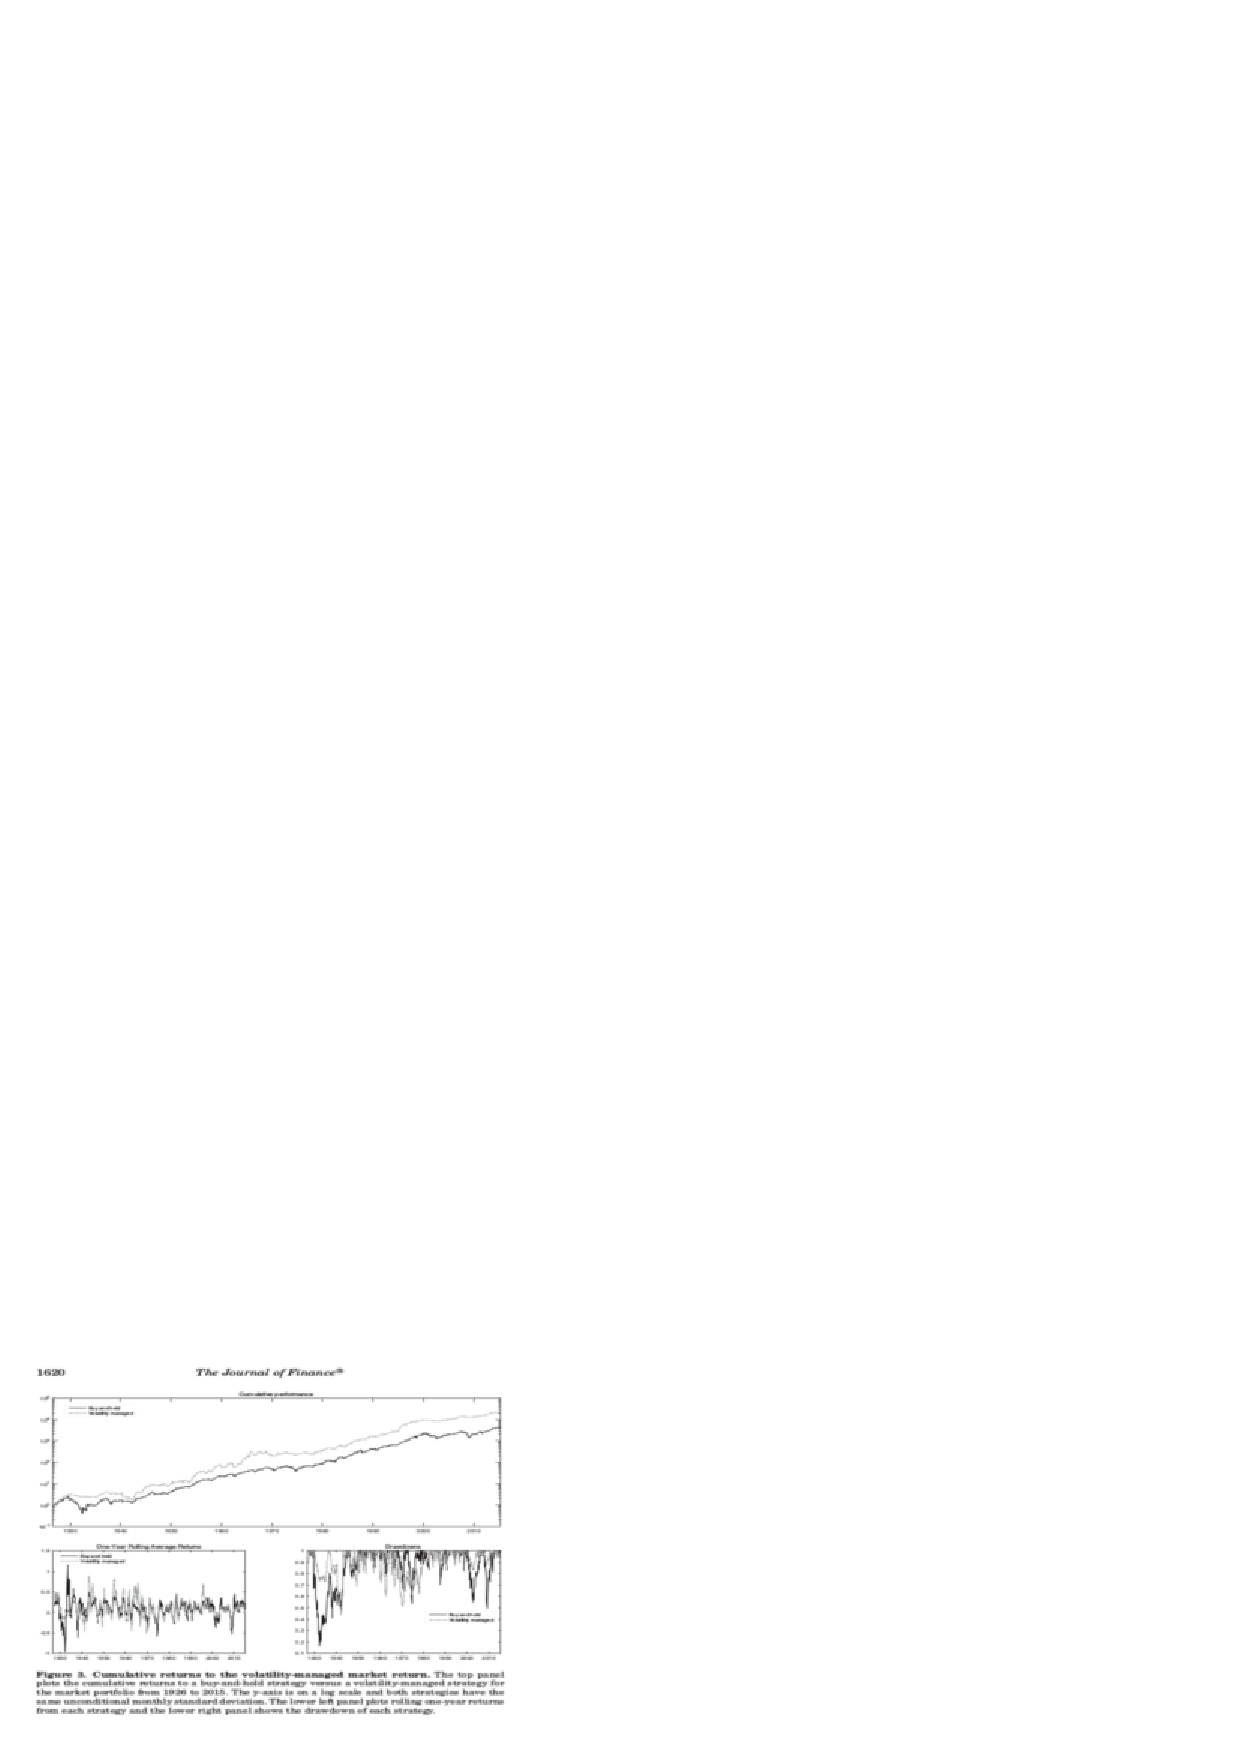
\includegraphics{mm}
%	\end{figure}
%
%\end{frame}

%\begin{frame}{Variance Decomposition}
%	\begin{itemize}[<+->]
%	\item[]	%\begin{block}{Market Variance}
%	Market Variance
%			\begin{itemize}[<+->]
%				\item Campbell, Lettau, and Xu (2001) - variance of individual assets vs market variance and CAPM
%				\item Pollet and Wilson (2010) - decompose quarterly variance of market portfolio - Avg cor and Avg var
%			\end{itemize}
%	%	\end{block}
%	\item[] Avg Var and Avg Cor
%	%	\begin{block}{Avg Var and Avg Cor}
%
%			\begin{align*}
%			R_{s,t} &= \sum_{1}^{N}w_{n,t}R_{n,t} \\
%			\sigma^{2}(r_{s,t}) &= \sum_{n=1}^{N} \sum_{m=1}^{N}w_{n,t}w_{m,t}\sigma^{2}_{n,t}\sigma^{2}_{m,t}\rho_{n,m,t}\\
%			\sigma^{2}_{s,t} &= \sum_{n=1}^{N} w_{n,t}\sigma^{2}_{n,t} \times \sum_{n=1}^{N}\sum_{m \neq n}^{N}w_{n,t}w_{m,t}\rho_{n,m,t}\\
%			AV_{t} &= \sum_{n=1}^{N} w_{n,t}\sigma^{2}_{n,t} ~ \text{ and } ~ AC_{t} = \sum_{n=1}^{N}\sum_{m \neq n}^{N}w_{n,t}w_{m,t}\rho_{n,m,t}
%			\end{align*}
%	%	\end{block}
%	\end{itemize}
%	
%\end{frame}

%\begin{frame}{Pollet and Wilson 2010 - Risk}
%		\vspace{-12pt}
%		\begin{table}
%			\caption{1963Q2:2007Q1}
%			\vspace{-18pt}
%			\begin{adjustbox}{width=\textwidth,height=3cm}
%				\input{tab_var_rep_4_presentation.tex}
%			\end{adjustbox}
%		\end{table}
%\end{frame}
%
%\begin{frame}{Pollet and Wilson 2010 - Returns}
%		\vspace{-12pt}
%		\begin{table}
%			\caption{1963Q2:2007Q1}
%			\vspace{-18pt}
%			\begin{adjustbox}{width=\textwidth,height=3cm}
%				
% Table created by stargazer v.5.2 by Marek Hlavac, Harvard University. E-mail: hlavac at fas.harvard.edu
% Date and time: Fri, Mar 30, 2018 - 12:18:38  IST
\begin{table}[!htbp] \centering 
  \caption{} 
  \label{} 
\begin{tabular}{@{\extracolsep{5pt}}lccccc} 
\\[-1.8ex]\hline 
\hline \\[-1.8ex] 
 & \multicolumn{5}{c}{\textit{Dependent variable:}} \\ 
\cline{2-6} 
\\[-1.8ex] & \multicolumn{5}{c}{RET$_{t+1}} \\ 
\\[-1.8ex] & (1) & (2) & (3) & (4) & (5)\\ 
\hline \\[-1.8ex] 
 AC$_{t}$ & 0.212$^{***}$ &  & 0.246$^{***}$ &  &  \\ 
  & (0.065) &  & (0.069) &  &  \\ 
  & & & & & \\ 
 AV$_{t}$ &  & $-$0.139 & $-$0.540 &  & $-$1.768$^{***}$ \\ 
  &  & (0.344) & (0.351) &  & (0.605) \\ 
  & & & & & \\ 
 SV$_{t}$ &  &  &  & 1.425 & 5.764$^{***}$ \\ 
  &  &  &  & (1.007) & (1.782) \\ 
  & & & & & \\ 
 Constant & $-$0.037$^{**}$ & 0.016 & $-$0.033$^{*}$ & 0.006 & 0.024$^{**}$ \\ 
  & (0.016) & (0.010) & (0.017) & (0.008) & (0.010) \\ 
  & & & & & \\ 
\hline \\[-1.8ex] 
Observations & 180 & 180 & 180 & 180 & 180 \\ 
R$^{2}$ & 0.056 & 0.001 & 0.068 & 0.011 & 0.057 \\ 
Adjusted R$^{2}$ & 0.050 & $-$0.005 & 0.058 & 0.006 & 0.046 \\ 
Residual Std. Error & 0.081 (df = 178) & 0.083 (df = 178) & 0.081 (df = 177) & 0.083 (df = 178) & 0.081 (df = 177) \\ 
F Statistic & 10.480$^{***}$ (df = 1; 178) & 0.165 (df = 1; 178) & 6.463$^{***}$ (df = 2; 177) & 2.002 (df = 1; 178) & 5.320$^{***}$ (df = 2; 177) \\ 
\hline 
\hline \\[-1.8ex] 
\textit{Note:}  & \multicolumn{5}{r}{$^{*}$p$<$0.1; $^{**}$p$<$0.05; $^{***}$p$<$0.01} \\ 
\end{tabular} 
\end{table} 

%			\end{adjustbox}
%		\end{table}
%\end{frame}

\begin{frame}{Average Variance}
	\begin{itemize}[<+->]
		\item Timing leverage by variance generates higher returns
		\item Market variance contains average correlation
		\item Average variance is at least unrelated to future returns
		\item $W_{t}$ = $\frac{1}{AV_{t-1}}$ is the investment weight on the CRSP market portfolio
	\end{itemize}
\end{frame}

%\section{Data}
%
%\begin{frame}{Data}
%	\begin{block}{CRSP daily returns}
%		\begin{itemize}
%			\item NYSE daily return (1926-2017)
%			\item NYSE-AMEX daily returns (1962-2017)
%			\item NASDAQ daily returns (1974-2017)
%			\item Monthly Variance Stats and MCAP of gaming industry
%		\end{itemize}
%	\end{block}
%	\begin{block}{Asaif Manela's Website}
%		\begin{itemize}
%			\item ICRF = $\frac{MarEqt}{MarEqt + BookDbt}$ He, Kelly, Manela (2017)
%			\item LF$_{AEM}$ = $\frac{FinAsst}{FinAsst - BankDbt}$ Adrian, Etula and Muir (2014)
%			\item BC = year on year increase in bank credit Gandhi (2016)
%		\end{itemize}
%	\end{block}
%	\begin{block}{NYSE}
%		\begin{itemize}
%			\item $\Delta$ MD = month to month change in Margin Debt
%		\end{itemize}
%	\end{block}	
%\end{frame}
%
%\section{Variance Decomposition}
%
%%\begin{frame}{Market Variance}
%%	\begin{align}
%%	%SV_{t} &= \frac{1}{t-1}\sum_{\tau = 1}^{t} \left(R^{m}_{\tau} - \frac{\sum_{\tau = 1}^{t} R^{m}_{\tau}}{t}\right)^{2}\\
%%	SV_{t} &= \sum_{n=1}^{N} \sum_{m=1}^{N}w^{n}_{t}w^{m}_{t}\sigma^{2}_{n,t}\sigma^{2}_{m,t}\rho^{n,m}_{t}\\
%%	SV_{t} &= \sum_{n=1}^{N} w^{n}_{t}\sigma^{2}_{n,t} \times \sum_{n=1}^{N}\sum_{m \neq n}^{N}w^{n}_{t}w^{m}_{t}\rho^{n,m}_{t}\\
%%	AV_{t} &= \sum_{n=1}^{N} w^{n}_{t}\sigma^{2}_{n,t}\\
%%	AC_{t} &= \sum_{n=1}^{N}\sum_{m \neq n}^{N}w^{n}_{t}w^{m}_{t}\rho^{n,m}_{t}\\
%%	\end{align}
%%\end{frame}
%
%\begin{frame}{Summary Stats}
%	\begin{table}[!htbp] \centering 
%		\begin{adjustbox}{width=\textwidth}
%			\begin{tabular}{lcccccc} 
%				%
% Table created by stargazer v.5.2 by Marek Hlavac, Harvard University. E-mail: hlavac at fas.harvard.edu
% Date and time: Fri, Mar 30, 2018 - 12:18:16  IST
\begin{table}[!htbp] \centering 
  \caption{} 
  \label{} 
\begin{tabular}{@{\extracolsep{5pt}}lccccc} 
\\[-1.8ex]\hline 
\hline \\[-1.8ex] 
Statistic & \multicolumn{1}{c}{N} & \multicolumn{1}{c}{Mean} & \multicolumn{1}{c}{St. Dev.} & \multicolumn{1}{c}{Min} & \multicolumn{1}{c}{Max} \\ 
\hline \\[-1.8ex] 
RET & 180 & 1.273 & 8.320 & $-$30.072 & 19.956 \\ 
AC & 180 & 0.233 & 0.093 & 0.034 & 0.648 \\ 
AV & 180 & 2.211 & 1.814 & 0.634 & 12.044 \\ 
SV & 180 & 0.489 & 0.616 & 0.029 & 6.397 \\ 
\hline \\[-1.8ex] 
\end{tabular} 
\end{table} 

%				%
% Table created by stargazer v.5.2 by Marek Hlavac, Harvard University. E-mail: hlavac at fas.harvard.edu
% Date and time: Mon, Mar 19, 2018 - 12:16:38  IST
\begin{table}[!htbp] \centering 
  \caption{} 
  \label{} 
\begin{tabular}{@{\extracolsep{5pt}}lccccc} 
\\[-1.8ex]\hline 
\hline \\[-1.8ex] 
Statistic & \multicolumn{1}{c}{N} & \multicolumn{1}{c}{Mean} & \multicolumn{1}{c}{St. Dev.} & \multicolumn{1}{c}{Min} & \multicolumn{1}{c}{Max} \\ 
\hline \\[-1.8ex] 
RET & 215 & 1.210 & 8.458 & $-$30.072 & 19.956 \\ 
AC & 215 & 0.261 & 0.113 & 0.034 & 0.678 \\ 
AV & 215 & 2.315 & 2.232 & 0.634 & 20.485 \\ 
SV & 215 & 0.600 & 1.007 & 0.029 & 11.378 \\ 
\hline \\[-1.8ex] 
\end{tabular} 
\end{table} 

%				
% Table created by stargazer v.5.2 by Marek Hlavac, Harvard University. E-mail: hlavac at fas.harvard.edu
% Date and time: Mon, Mar 05, 2018 - 05:40:49  IST 
& \multicolumn{6}{c}{Monthly 1962M6:2016M12}
\\\hline 
\hline \\[-1.8ex] 
Statistic & \multicolumn{1}{c}{N} & \multicolumn{1}{c}{Mean} & \multicolumn{1}{c}{St. Dev.} & \multicolumn{1}{c}{Min} & \multicolumn{1}{c}{Max} & \multicolumn{1}{c}{Autocorrelation}\\ 
\hline \\[-1.8ex] 
RET & 655 & 0.410 & 4.460 & $-$26.134 & 14.814 & 0.081\\ 
AC & 655 & 0.261 & 0.129 & 0.019 & 0.762 & 0.620\\ 
AV & 655 & 0.770 & 0.849 & 0.198 & 10.416 & 0.667\\ 
SV & 655 & 0.200 & 0.406 & 0.006 & 5.664 & 0.551\\ 
\hline\\[-1.8ex] 
& \multicolumn{6}{c}{Monthly 1926M7:2016M12}\\
\hline \hline\\[-1.8ex] 
Statistic & \multicolumn{1}{c}{N} & \multicolumn{1}{c}{Mean} & \multicolumn{1}{c}{St. Dev.} & \multicolumn{1}{c}{Min} & \multicolumn{1}{c}{Max} & \multicolumn{1}{c}{Autocorrelation}\\ 
\hline \\[-1.8ex] 
RET & 1,085 & 0.495 & 5.371 & $-$34.523 & 33.188 & 0.106\\ 
AC & 1,085 & 0.276 & 0.134 & 0.019 & 0.762 & 0.610\\ 
AV & 1,085 & 0.881 & 1.281 & 0.154 & 19.540 &  0.718\\ 
SV & 1,085 & 0.248 & 0.502 & 0.006 & 5.808 & 0.612\\ 
\hline \\[-1.8ex] 

%			\end{tabular}
%		\end{adjustbox}
%	\end{table}
%\end{frame}


\section{Results}
\subsection{In Sample}

\begin{frame}{Variance Prediction}
	\vspace{-12pt}
 \begin{table}
 	\begin{adjustbox}{width=\textwidth,height=4cm}
 	
% Table created by stargazer v.5.2 by Marek Hlavac, Harvard University. E-mail: hlavac at fas.harvard.edu
% Date and time: Fri, Jun 08, 2018 - 01:01:25  IST
\begin{tabular}{@{\extracolsep{5pt}}lccccc} 
\\[-1.8ex]\hline 
\hline \\[-1.8ex] 
\\[-1.8ex] & \multicolumn{5}{c}{SV$_{t+1}$} \\ 
\hline \\[-1.8ex] 
 AV & 0.545$^{***}$ &  &  & 0.489$^{***}$ & 0.257$^{***}$ \\ 
  & p = 0.000 &  &  & p = 0.000 & p = 0.001 \\ 
  & & & & & \\ 
 AC &  & 0.332$^{***}$ &  & 0.160$^{***}$ &  \\ 
  &  & p = 0.000 &  & p = 0.00001 &  \\ 
  & & & & & \\ 
 SV &  &  & 0.551$^{***}$ &  & 0.320$^{***}$ \\ 
  &  &  & p = 0.000 &  & p = 0.00002 \\ 
  & & & & & \\ 
 Constant & $-$0.0005 & $-$0.0001 & $-$0.0003 & $-$0.0005 & $-$0.0004 \\ 
  & p = 0.989 & p = 0.999 & p = 0.993 & p = 0.989 & p = 0.991 \\ 
  & & & & & \\ 
\textit{N} & 654 & 654 & 654 & 654 & 654 \\ 
R$^{2}$ & 0.297 & 0.110 & 0.304 & 0.320 & 0.317 \\ 
Adjusted R$^{2}$ & 0.296 & 0.109 & 0.303 & 0.318 & 0.315 \\ 
\hline 
\hline \\[-1.8ex] 
\textit{Notes:} & \multicolumn{5}{r}{$^{***}$Significant at the 1 percent level.} \\ 
 & \multicolumn{5}{r}{$^{**}$Significant at the 5 percent level.} \\ 
 & \multicolumn{5}{r}{$^{*}$Significant at the 10 percent level.} \\ 
\end{tabular} 

 	\end{adjustbox}

 \end{table}
\end{frame}

%\begin{frame}{AV Prediction}
%	\vspace{-12pt}
%	\begin{table}
%		\begin{adjustbox}{width=\textwidth,height=4cm}
%			
% Table created by stargazer v.5.2 by Marek Hlavac, Harvard University. E-mail: hlavac at fas.harvard.edu
% Date and time: Mon, Mar 26, 2018 - 11:55:30  IST
%\begin{table}[!htbp] \centering 
%  \caption{} 
%  \label{} 
\begin{tabular}{lccccc} 
	\multicolumn{6}{c}{Sample 1962M6:2016M12}\\
	\hline\\
	& \multicolumn{5}{c}{AV$_{t+1}$} \\ 
	\\[-1.8ex] 
	\hline \\[-1.8ex] 
 AC$_{t}$ & 0.014$^{***}$ &  &  & $-$0.001 &  \\ 
  & (0.003) &  &  & (0.002) &  \\ 
  & & & & & \\ 
 AV$_{t}$ &  & 0.667$^{***}$ &  & 0.674$^{***}$ & 1.030$^{***}$ \\ 
  &  & (0.029) &  & (0.031) & (0.065) \\ 
  & & & & & \\ 
 SV$_{t}$ &  &  & 1.092$^{***}$ &  & $-$0.844$^{***}$ \\ 
  &  &  & (0.070) &  & (0.135) \\ 
  & & & & & \\ 
 Constant & 0.004$^{***}$ & 0.003$^{***}$ & 0.006$^{***}$ & 0.003$^{***}$ & 0.001$^{***}$ \\ 
  & (0.001) & (0.0003) & (0.0003) & (0.001) & (0.0004) \\ 
  & & & & & \\ 
\hline \\[-1.8ex] 
Observations & 654 & 654 & 654 & 654 & 654 \\ 
R$^{2}$ & 0.048 & 0.445 & 0.273 & 0.446 & 0.477 \\ 
Adjusted R$^{2}$ & 0.046 & 0.445 & 0.272 & 0.444 & 0.475 \\ 
%Residual Std. Error & 0.008 (df = 652) & 0.006 (df = 652) & 0.007 (df = 652) & 0.006 (df = 651) & 0.006 (df = 651) \\ 
%F Statistic & 32.601$^{***}$ (df = 1; 652) & 523.763$^{***}$ (df = 1; 652) & 244.654$^{***}$ (df = 1; 652) & 261.813$^{***}$ (df = 2; 651) & 296.603$^{***}$ (df = 2; 651) \\ 
\hline 
\hline \\[-1.8ex] 
\textit{Note:}  & \multicolumn{5}{r}{$^{*}$p$<$0.1; $^{**}$p$<$0.05; $^{***}$p$<$0.01} \\ 
\end{tabular} 
%\end{table} 

%		\end{adjustbox}
%		
%	\end{table}
%\end{frame}

\begin{frame}{Return Prediction}
	\vspace{-12pt}
	\begin{table}
		\begin{adjustbox}{width=\textwidth,height=4cm}
			
% Table created by stargazer v.5.2 by Marek Hlavac, Harvard University. E-mail: hlavac at fas.harvard.edu
% Date and time: Fri, Jun 08, 2018 - 01:03:43  IST
\begin{tabular}{@{\extracolsep{5pt}}lccccc} 
%\\[-1.8ex]\hline 
%\hline \\[-1.8ex] 
%\\[-1.8ex] & \multicolumn{5}{c}{RET$_{t+1}$} \\ 
\\[-1.8ex]
\hline \\[-1.8ex] 
 AV & $-$0.130$^{***}$ &  &  & $-$0.168$^{***}$ & $-$0.173$^{*}$ \\ 
  & p = 0.001 &  &  & p = 0.0001 & p = 0.052 \\ 
%  & & & & & \\ 
 AC &  & 0.049 &  & 0.108$^{***}$ &  \\ 
  &  & p = 0.212 &  & p = 0.010 &  \\ 
%  & & & & & \\ 
 SV &  &  & $-$0.107$^{***}$ &  & 0.048 \\ 
  &  &  & p = 0.006 &  & p = 0.588 \\ 
%  & & & & & \\ 
 Constant & $-$0.000 & $-$0.000 & $-$0.000 & $-$0.000 & $-$0.000 \\ 
  & p = 1.000 & p = 1.000 & p = 1.000 & p = 1.000 & p = 1.000 \\ 
%  & & & & & \\ 
\textit{N} & 655 & 655 & 655 & 655 & 655 \\ 
R$^{2}$ & 0.017 & 0.002 & 0.012 & 0.027 & 0.017 \\ 
Adjusted R$^{2}$ & 0.015 & 0.001 & 0.010 & 0.024 & 0.014 \\ 
%\hline 
\hline \\[-1.8ex] 
\textit{Notes:} & \multicolumn{5}{r}{$^{***}$,$^{**}$, and $^{*}$ Significant at the 1, 5, and 10 percent levels.} \\ 
% & \multicolumn{5}{r}{$^{**}$Significant at the 5 percent level.} \\ 
% & \multicolumn{5}{r}{$^{*}$Significant at the 10 percent level.} \\ 
\end{tabular} 

		\end{adjustbox}
		
	\end{table}
\end{frame}

%\begin{frame}{Risk vs Return}
%	\vspace{-12pt}
%	\begin{table}
%		\caption{1962M7:2016M12}
%		\vspace{-6pt}
%		\begin{adjustbox}{width=10cm,height=4cm}
%			
% Table created by stargazer v.5.2 by Marek Hlavac, Harvard University. E-mail: hlavac at fas.harvard.edu
% Date and time: Fri, Mar 30, 2018 - 12:18:42  IST
\begin{table}[!htbp] \centering 
  \caption{} 
  \label{} 
\begin{tabular}{@{\extracolsep{5pt}}lcccccccccccc} 
\\[-1.8ex]\hline 
\hline \\[-1.8ex] 
 & \multicolumn{12}{c}{\textit{Dependent variable:}} \\ 
\cline{2-13} 
\\[-1.8ex] & \multicolumn{3}{c}{RET$_{t+1}$} & \multicolumn{3}{c}{RET$_{t+3}$} & \multicolumn{3}{c}{RET$_{t+6}$} & \multicolumn{3}{c}{RET$_{t+12}$} \\ 
\\[-1.8ex] & (1) & (2) & (3) & (4) & (5) & (6) & (7) & (8) & (9) & (10) & (11) & (12)\\ 
\hline \\[-1.8ex] 
 AV$_{t}$ & $-$0.678$^{***}$ &  & $-$0.905$^{*}$ & $-$0.973$^{***}$ &  & $-$3.000$^{***}$ & $-$0.790 &  & $-$6.457$^{***}$ & $-$1.027 &  & $-$11.873$^{***}$ \\ 
  & (0.203) &  & (0.463) & (0.368) &  & (0.835) & (0.538) &  & (1.203) & (0.758) &  & (1.666) \\ 
  & & & & & & & & & & & & \\ 
 SV$_{t}$ &  & $-$1.174$^{***}$ & 0.526 &  & $-$0.923 & 4.711$^{***}$ &  & 1.046 & 13.171$^{***}$ &  & 2.900$^{*}$ & 25.203$^{***}$ \\ 
  &  & (0.426) & (0.969) &  & (0.772) & (1.744) &  & (1.124) & (2.512) &  & (1.581) & (3.480) \\ 
  & & & & & & & & & & & & \\ 
 Constant & 0.009$^{***}$ & 0.007$^{***}$ & 0.010$^{***}$ & 0.020$^{***}$ & 0.014$^{***}$ & 0.026$^{***}$ & 0.031$^{***}$ & 0.023$^{***}$ & 0.048$^{***}$ & 0.056$^{***}$ & 0.042$^{***}$ & 0.089$^{***}$ \\ 
  & (0.002) & (0.002) & (0.003) & (0.004) & (0.003) & (0.005) & (0.006) & (0.005) & (0.007) & (0.009) & (0.007) & (0.010) \\ 
  & & & & & & & & & & & & \\ 
\hline \\[-1.8ex] 
Observations & 655 & 655 & 655 & 652 & 652 & 652 & 649 & 649 & 649 & 643 & 643 & 643 \\ 
R$^{2}$ & 0.017 & 0.012 & 0.017 & 0.011 & 0.002 & 0.022 & 0.003 & 0.001 & 0.044 & 0.003 & 0.005 & 0.078 \\ 
Adjusted R$^{2}$ & 0.015 & 0.010 & 0.014 & 0.009 & 0.001 & 0.019 & 0.002 & $-$0.0002 & 0.041 & 0.001 & 0.004 & 0.076 \\ 
Residual Std. Error & 0.044 (df = 653) & 0.044 (df = 653) & 0.044 (df = 652) & 0.080 (df = 650) & 0.080 (df = 650) & 0.079 (df = 649) & 0.117 (df = 647) & 0.117 (df = 647) & 0.114 (df = 646) & 0.164 (df = 641) & 0.164 (df = 641) & 0.158 (df = 640) \\ 
F Statistic & 11.164$^{***}$ (df = 1; 653) & 7.605$^{***}$ (df = 1; 653) & 5.723$^{***}$ (df = 2; 652) & 7.011$^{***}$ (df = 1; 650) & 1.432 (df = 1; 650) & 7.186$^{***}$ (df = 2; 649) & 2.157 (df = 1; 647) & 0.866 (df = 1; 647) & 14.866$^{***}$ (df = 2; 646) & 1.836 (df = 1; 641) & 3.363$^{*}$ (df = 1; 641) & 27.219$^{***}$ (df = 2; 640) \\ 
\hline 
\hline \\[-1.8ex] 
\textit{Note:}  & \multicolumn{12}{r}{$^{*}$p$<$0.1; $^{**}$p$<$0.05; $^{***}$p$<$0.01} \\ 
\end{tabular} 
\end{table} 

%		\end{adjustbox}
%	\end{table}
%\end{frame}

\subsection{Out of Sample}
%\begin{frame}{Out-of-Sample Tests}
%	\begin{itemize}[<+->]
%		\item Divide the sample 1962:06 - 2016:12 into 15\% training 85\% prediction
%		\begin{itemize}
%			\item Initial training period $t = q$ months. First ~8 years.
%			\item Remaining period $t = q+1, q+2,..,T$ for out-of-sample forecast evaluation.
%		\end{itemize}
%		\item Regression model is "trained" over initial period
%		\begin{itemize}
%			\item Estimate $\hat \alpha_{t}$ and $\hat \beta_{t}$ by regressing $\{r_{s+1}\}_{s=1}^{t-1}$ on a constant and $\{x\}_{s=1}^{t-1}$
%		\end{itemize}
%		\item Generate one period ahead prediction \\
%		\begin{itemize}
%			\item $\hat r_{t+1} = \hat \alpha_{t} + \hat \beta_{t}x_{t}$
%		\end{itemize}
%		\item Each following month the ``training" window expands by one month
%	\end{itemize}
%\end{frame}
%
%\begin{frame}{Out of Sample Stats}
%	    \begin{itemize}
%	    	\item y$_{t}$ - $\hat{y}_{x,t}$ =  $e_{x,t}$ : forecast error of preditor x
%	    	\item $\frac{1}{T}\sum_{1}^{T}(e_{x,t})^{2}$ = MSFE$_{x}$: mean squared forecast error based on predictor $x$
%	    \end{itemize}
%	    \begin{block}{$R_{oos}^{2}$ Campbell and Thompson 2007}
%	    	\begin{itemize}
%	    		\item $R^{2}_{os}$ = 1 - $\frac{MSFE_{x}}{MSFE_{b}}$
%	    		\item $R^{2}_{os}$ = proportional reduction in MSFE
%	    	\end{itemize}
%	    \end{block}
%	    \begin{block}{MSE-F Mcracken 2004}
%	    	\begin{itemize}
%	    		\item MSE-F = $T \times \frac{\frac{1}{T}\sum_{1}^{T}(e_{b,t}^{2}-e_{x,t}^{2})}{MSFE_{x}}$
%	    		\item MSE-F = F-type test for significance in squared residual (like in sample regression)
%	    	\end{itemize}
%	    \end{block}
%\end{frame}
%
%\begin{frame}{Out of Sample Stats}
%	\begin{itemize}
%		\item $R_{oos}^{2}$ and MSE-F test improvement in forecast accuracy relative to a benchmark
%		\item Encompassing tests impose the greater requirement that the benchmark have no valuable forecasting information
%	\end{itemize}
%	\begin{block}{ENC-NEW Mcracken and Clark 2009}
%		\begin{itemize}
%			\item ENC-NEW = $T\times \frac{\frac{1}{T}\sum_{1}^{T}(e_{b,t}^{2}-e_{b,t}e_{x,t})}{MSFE_{x}}$
%			\item ENC-NEW = F-type statistic on the imporvement of including the benchmark
%		\end{itemize}
%	\end{block}
%	\begin{block}{ENC-HLN Harvey, Lebourne and Newbold 1998}
%		\begin{itemize}
%			\item Optimal forecast = $\hat{y}^{*}_{t} = (1-\lambda)\hat{y}_{b,t} + \lambda \hat{y}_{x,t}$
%			\item $\lambda$ = measure of the optimal combination of forecasts from x and the benchmark
%		\end{itemize}
%	\end{block}
%\end{frame}
%
%\begin{frame}{Out of Sample Results}
%	\vspace{-12pt}
%	\begin{table}
%		\caption{1970M7:2016M12}
%		\vspace{-6pt}
%		\begin{adjustbox}{width=\textwidth}
%			% Table created by stargazer v.5.2 by Marek Hlavac, Harvard University. E-mail: hlavac at fas.harvard.edu
% Date and time: Wed, Mar 07, 2018 - 02:47:43  IST
\begin{table}[!htbp] \centering 
	\caption{} 
	\label{} 
	\begin{tabular}{@{\extracolsep{5pt}} ccccHcc} 
		\\[-1.8ex]\hline 
		\hline \\[-1.8ex] 
		 & Sample & $R{2}_{oos}$ & MSE-F & DM & ENC-NEW & ENC-HLN \\ 
		\hline \\[-1.8ex] 
		SV$_{t+1}$ & 1963Q2:2007Q1 & 11.912**  & 12.846*** & 1.441*  & 17.937**  & 0.779** *  \\ 
		SV$_{t+1}$ & Quarterly & 35.041** *  & 147.267*** & 2.554** *  & 163.112**  & 0.911** *  \\ 
		SV$_{t+1}$ & Monthly & 37.858**  & 496.516*** & 2.495** *  & 582.268**  & 0.872** *  \\ 
		RET$_{t+1}$ & 1963Q2:2007Q1 & -7.311 & -6.472 & -1.413 & 0.302 & 0.043 \\ 
		RET$_{t+1}$ & Quarterly & -0.358 & -0.975 & -0.237 & 0.898**  & 0.324 \\ 
		RET$_{t+1}$ & Monthly & 0.636 & 5.220*** & 1.014 & 3.706**  & 1*  \\ 
		\hline \\[-1.8ex] 
		\\[-1.8ex]\hline 
		\hline \\[-1.8ex] 
		variable & Sample & $R^{2}_{oos}$ & MSE-F & DM & ENC-NEW & ENC-HLN \\ 
		\hline \\[-1.8ex] 
		SV$_{t+1}$ & 1963Q2:2007Q1 & 15.135**  & 16.942*** & 1.814**  & 12.563**  & 1**  \\ 
		SV$_{t+1}$ & Quarterly & 8.769**  & 26.239*** & 1.292*  & 29.585**  & 0.898** *  \\ 
		SV$_{t+1}$ & Monthly & 2.793**  & 23.417*** & 0.251 & 109.745**  & 0.56**  \\ 
		RET$_{t+1}$ & 1963Q2:2007Q1 & 15.307 & 17.170*** & 0.838 & 15.152**  & 1 \\ 
		RET$_{t+1}$ & Quarterly & 0.746 & 2.052** & 0.582 & 1.866**  & 1 \\ 
		RET$_{t+1}$ & Monthly & 0.178 & 1.454* & 0.765 & 0.9**  & 1 \\ 
		\hline \\[-1.8ex] 
	\end{tabular} 
\end{table} 
%		\end{adjustbox}
%	\end{table}
%\end{frame}

\begin{frame}{Out of Sample Results}
	\vspace{-12pt}
	\begin{table}
		\caption{Sample 1970:07 to 2016:12}
		\vspace{-6pt}
		\begin{adjustbox}{center,max height=\totalheight}
			
% Table created by stargazer v.5.2 by Marek Hlavac, Harvard University. E-mail: hlavac at fas.harvard.edu
% Date and time: Sun, Jun 10, 2018 - 12:59:08  IST
\begin{table}[!htbp] \centering 
  \caption{} 
  \label{} 
\begin{tabular}{@{\extracolsep{5pt}} cccc} 
\\[-1.8ex]\hline 
\hline \\[-1.8ex] 
variable & DM & MSE-F & ENC-HLN \\ 
\hline \\[-1.8ex] 
AC\$\_\{t+1\}\$ & -1.627 & -144.647 & 0 \\ 
SV\$\_\{t+1\}\$ & -1.631 & -27.854 & 0 \\ 
AV\$\_\{t+1\}\$ & -2.39 & -55.67 & 0 \\ 
RET\$\_\{t+1\}\$ & -0.238 & -1.533 & 0.265 \\ 
AC\$\_\{t+1\}\$ & 1.074 & 109.736\textasteriskcentered \textasteriskcentered \textasteriskcentered  & 1 \\ 
SV\$\_\{t+1\}\$ & 1.53\textasteriskcentered  & 29.252\textasteriskcentered \textasteriskcentered \textasteriskcentered  & 1\textasteriskcentered \textasteriskcentered  \\ 
AV\$\_\{t+1\}\$ & 2.286\textasteriskcentered \textasteriskcentered  & 109.333\textasteriskcentered \textasteriskcentered \textasteriskcentered  & 1\textasteriskcentered \textasteriskcentered \textasteriskcentered  \\ 
RET\$\_\{t+1\}\$ & 1.278 & 11.801\textasteriskcentered \textasteriskcentered \textasteriskcentered  & 1\textasteriskcentered  \\ 
\hline \\[-1.8ex] 
\end{tabular} 
\end{table} 

		\end{adjustbox}
	\end{table}
\end{frame}

\begin{frame}{Out of Sample Results}
	\vspace{-12pt}
	\begin{table}
		\caption{Sample 1939:12 to 2016:12}
		\vspace{-6pt}
		\begin{adjustbox}{center,max height=\totalheight}
			
% Table created by stargazer v.5.2 by Marek Hlavac, Harvard University. E-mail: hlavac at fas.harvard.edu
% Date and time: Sat, Apr 07, 2018 - 01:04:28  IST
\begin{table}[!htbp] \centering 
  \caption{} 
  \label{} 
\begin{tabular}{@{\extracolsep{5pt}} cccc} 
\\[-1.8ex]\hline 
\hline \\[-1.8ex] 
variable & DM & MSE-F & ENC-HLN \\ 
\hline \\[-1.8ex] 
AC\$\_\{t+1\}\$ & -2.2 & -36.182 & 0.075 \\ 
SV\$\_\{t+1\}\$ & -0.431 & -8.453 & 0.403 \\ 
AV\$\_\{t+1\}\$ & -2.374 & -12.431 & 0\textasteriskcentered \textasteriskcentered \textasteriskcentered  \\ 
RET\$\_\{t+1\}\$ & -1.766 & -4.832 & 0\textasteriskcentered \textasteriskcentered \textasteriskcentered  \\ 
AC\$\_\{t+1\}\$ & 1.604\textasteriskcentered  & 46.251\textasteriskcentered \textasteriskcentered \textasteriskcentered  & 1 \\ 
SV\$\_\{t+1\}\$ & 1.041 & 21.57\textasteriskcentered \textasteriskcentered \textasteriskcentered  & 0.956 \\ 
AV\$\_\{t+1\}\$ & 3.104\textasteriskcentered \textasteriskcentered \textasteriskcentered  & 198.267\textasteriskcentered \textasteriskcentered \textasteriskcentered  & 1 \\ 
RET\$\_\{t+1\}\$ & -2.027 & -8.702 & 0\textasteriskcentered \textasteriskcentered \textasteriskcentered  \\ 
\hline \\[-1.8ex] 
\end{tabular} 
\end{table} 

		\end{adjustbox}
	\end{table}
\end{frame}

\section{Asset Allocation}

\begin{frame}{Returns}
	\begin{adjustbox}{width=\textwidth,height=.8\textheight}
		% Created by tikzDevice version 0.10.1 on 2018-03-26 14:40:36
% !TEX encoding = UTF-8 Unicode
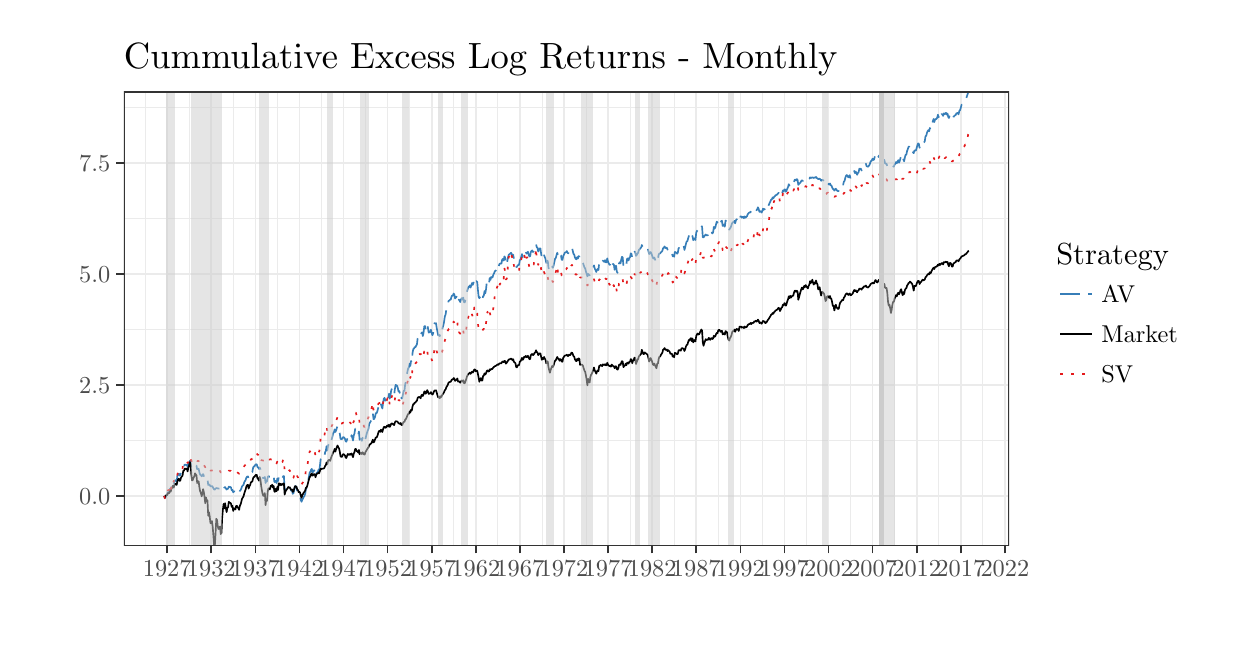
\begin{tikzpicture}[x=1pt,y=1pt]
\definecolor{fillColor}{RGB}{255,255,255}
\path[use as bounding box,fill=fillColor,fill opacity=0.00] (0,0) rectangle (426.79,216.81);
\begin{scope}
\path[clip] (  0.00,  0.00) rectangle (426.79,216.81);
\definecolor{drawColor}{RGB}{255,255,255}
\definecolor{fillColor}{RGB}{255,255,255}

\path[draw=drawColor,line width= 0.6pt,line join=round,line cap=round,fill=fillColor] (  0.00,  0.00) rectangle (426.79,216.81);
\end{scope}
\begin{scope}
\path[clip] ( 34.77, 29.59) rectangle (354.63,193.67);
\definecolor{fillColor}{RGB}{255,255,255}

\path[fill=fillColor] ( 34.77, 29.59) rectangle (354.63,193.67);
\definecolor{drawColor}{gray}{0.92}

\path[draw=drawColor,line width= 0.3pt,line join=round] ( 34.77, 67.61) --
	(354.63, 67.61);

\path[draw=drawColor,line width= 0.3pt,line join=round] ( 34.77,107.75) --
	(354.63,107.75);

\path[draw=drawColor,line width= 0.3pt,line join=round] ( 34.77,147.89) --
	(354.63,147.89);

\path[draw=drawColor,line width= 0.3pt,line join=round] ( 34.77,188.02) --
	(354.63,188.02);

\path[draw=drawColor,line width= 0.3pt,line join=round] ( 42.44, 29.59) --
	( 42.44,193.67);

\path[draw=drawColor,line width= 0.3pt,line join=round] ( 58.37, 29.59) --
	( 58.37,193.67);

\path[draw=drawColor,line width= 0.3pt,line join=round] ( 74.31, 29.59) --
	( 74.31,193.67);

\path[draw=drawColor,line width= 0.3pt,line join=round] ( 90.24, 29.59) --
	( 90.24,193.67);

\path[draw=drawColor,line width= 0.3pt,line join=round] (106.17, 29.59) --
	(106.17,193.67);

\path[draw=drawColor,line width= 0.3pt,line join=round] (122.10, 29.59) --
	(122.10,193.67);

\path[draw=drawColor,line width= 0.3pt,line join=round] (138.04, 29.59) --
	(138.04,193.67);

\path[draw=drawColor,line width= 0.3pt,line join=round] (153.97, 29.59) --
	(153.97,193.67);

\path[draw=drawColor,line width= 0.3pt,line join=round] (169.90, 29.59) --
	(169.90,193.67);

\path[draw=drawColor,line width= 0.3pt,line join=round] (185.83, 29.59) --
	(185.83,193.67);

\path[draw=drawColor,line width= 0.3pt,line join=round] (201.77, 29.59) --
	(201.77,193.67);

\path[draw=drawColor,line width= 0.3pt,line join=round] (217.70, 29.59) --
	(217.70,193.67);

\path[draw=drawColor,line width= 0.3pt,line join=round] (233.63, 29.59) --
	(233.63,193.67);

\path[draw=drawColor,line width= 0.3pt,line join=round] (249.57, 29.59) --
	(249.57,193.67);

\path[draw=drawColor,line width= 0.3pt,line join=round] (265.50, 29.59) --
	(265.50,193.67);

\path[draw=drawColor,line width= 0.3pt,line join=round] (281.44, 29.59) --
	(281.44,193.67);

\path[draw=drawColor,line width= 0.3pt,line join=round] (297.37, 29.59) --
	(297.37,193.67);

\path[draw=drawColor,line width= 0.3pt,line join=round] (313.30, 29.59) --
	(313.30,193.67);

\path[draw=drawColor,line width= 0.3pt,line join=round] (329.23, 29.59) --
	(329.23,193.67);

\path[draw=drawColor,line width= 0.3pt,line join=round] (345.17, 29.59) --
	(345.17,193.67);

\path[draw=drawColor,line width= 0.6pt,line join=round] ( 34.77, 47.54) --
	(354.63, 47.54);

\path[draw=drawColor,line width= 0.6pt,line join=round] ( 34.77, 87.68) --
	(354.63, 87.68);

\path[draw=drawColor,line width= 0.6pt,line join=round] ( 34.77,127.82) --
	(354.63,127.82);

\path[draw=drawColor,line width= 0.6pt,line join=round] ( 34.77,167.95) --
	(354.63,167.95);

\path[draw=drawColor,line width= 0.6pt,line join=round] ( 50.41, 29.59) --
	( 50.41,193.67);

\path[draw=drawColor,line width= 0.6pt,line join=round] ( 66.34, 29.59) --
	( 66.34,193.67);

\path[draw=drawColor,line width= 0.6pt,line join=round] ( 82.28, 29.59) --
	( 82.28,193.67);

\path[draw=drawColor,line width= 0.6pt,line join=round] ( 98.21, 29.59) --
	( 98.21,193.67);

\path[draw=drawColor,line width= 0.6pt,line join=round] (114.14, 29.59) --
	(114.14,193.67);

\path[draw=drawColor,line width= 0.6pt,line join=round] (130.07, 29.59) --
	(130.07,193.67);

\path[draw=drawColor,line width= 0.6pt,line join=round] (146.01, 29.59) --
	(146.01,193.67);

\path[draw=drawColor,line width= 0.6pt,line join=round] (161.94, 29.59) --
	(161.94,193.67);

\path[draw=drawColor,line width= 0.6pt,line join=round] (177.87, 29.59) --
	(177.87,193.67);

\path[draw=drawColor,line width= 0.6pt,line join=round] (193.80, 29.59) --
	(193.80,193.67);

\path[draw=drawColor,line width= 0.6pt,line join=round] (209.74, 29.59) --
	(209.74,193.67);

\path[draw=drawColor,line width= 0.6pt,line join=round] (225.67, 29.59) --
	(225.67,193.67);

\path[draw=drawColor,line width= 0.6pt,line join=round] (241.60, 29.59) --
	(241.60,193.67);

\path[draw=drawColor,line width= 0.6pt,line join=round] (257.53, 29.59) --
	(257.53,193.67);

\path[draw=drawColor,line width= 0.6pt,line join=round] (273.47, 29.59) --
	(273.47,193.67);

\path[draw=drawColor,line width= 0.6pt,line join=round] (289.40, 29.59) --
	(289.40,193.67);

\path[draw=drawColor,line width= 0.6pt,line join=round] (305.33, 29.59) --
	(305.33,193.67);

\path[draw=drawColor,line width= 0.6pt,line join=round] (321.26, 29.59) --
	(321.26,193.67);

\path[draw=drawColor,line width= 0.6pt,line join=round] (337.20, 29.59) --
	(337.20,193.67);

\path[draw=drawColor,line width= 0.6pt,line join=round] (353.13, 29.59) --
	(353.13,193.67);
\definecolor{drawColor}{RGB}{55,126,184}

\path[draw=drawColor,line width= 0.6pt,dash pattern=on 7pt off 3pt ,line join=round] ( 49.31, 47.61) --
	( 49.58, 46.82) --
	( 49.84, 47.22) --
	( 50.11, 47.85) --
	( 50.37, 47.83) --
	( 50.64, 48.93) --
	( 50.91, 48.96) --
	( 51.16, 49.05) --
	( 51.43, 50.24) --
	( 51.69, 49.70) --
	( 51.96, 51.16) --
	( 52.22, 51.62) --
	( 52.49, 52.47) --
	( 52.76, 51.59) --
	( 53.02, 52.85) --
	( 53.29, 53.30) --
	( 53.56, 53.18) --
	( 53.83, 52.79) --
	( 54.10, 54.88) --
	( 54.35, 55.42) --
	( 54.62, 55.62) --
	( 54.88, 55.00) --
	( 55.15, 55.05) --
	( 55.41, 56.24) --
	( 55.68, 56.69) --
	( 55.95, 56.95) --
	( 56.22, 58.52) --
	( 56.49, 58.53) --
	( 56.75, 58.89) --
	( 57.02, 58.88) --
	( 57.29, 58.74) --
	( 57.53, 58.87) --
	( 57.80, 58.09) --
	( 58.07, 58.97) --
	( 58.34, 59.42) --
	( 58.60, 60.28) --
	( 58.87, 59.80) --
	( 59.14, 57.72) --
	( 59.40, 57.59) --
	( 59.67, 57.61) --
	( 59.93, 57.83) --
	( 60.20, 58.08) --
	( 60.47, 58.99) --
	( 60.72, 58.73) --
	( 60.99, 58.52) --
	( 61.25, 57.25) --
	( 61.52, 57.41) --
	( 61.78, 57.42) --
	( 62.05, 56.09) --
	( 62.32, 55.27) --
	( 62.59, 55.15) --
	( 62.86, 54.71) --
	( 63.12, 54.98) --
	( 63.39, 55.50) --
	( 63.66, 54.82) --
	( 63.90, 54.13) --
	( 64.17, 53.56) --
	( 64.43, 54.02) --
	( 64.71, 53.84) --
	( 64.97, 53.86) --
	( 65.24, 51.55) --
	( 65.51, 51.74) --
	( 65.77, 51.62) --
	( 66.04, 51.07) --
	( 66.30, 51.05) --
	( 66.57, 51.17) --
	( 66.84, 50.91) --
	( 67.10, 50.40) --
	( 67.37, 49.92) --
	( 67.63, 49.91) --
	( 67.90, 50.28) --
	( 68.16, 50.45) --
	( 68.43, 50.41) --
	( 68.70, 50.30) --
	( 68.96, 50.23) --
	( 69.23, 50.34) --
	( 69.49, 50.36) --
	( 69.77, 49.49) --
	( 70.04, 49.61) --
	( 70.28, 50.13) --
	( 70.55, 50.50) --
	( 70.81, 50.85) --
	( 71.08, 50.60) --
	( 71.34, 50.80) --
	( 71.61, 50.28) --
	( 71.89, 49.92) --
	( 72.15, 50.15) --
	( 72.42, 50.24) --
	( 72.68, 50.96) --
	( 72.95, 50.81) --
	( 73.22, 50.84) --
	( 73.46, 50.69) --
	( 73.73, 49.63) --
	( 74.00, 49.80) --
	( 74.27, 48.93) --
	( 74.53, 49.21) --
	( 74.80, 49.20) --
	( 75.07, 49.04) --
	( 75.33, 49.68) --
	( 75.60, 49.71) --
	( 75.86, 49.39) --
	( 76.13, 49.14) --
	( 76.40, 48.71) --
	( 76.65, 49.37) --
	( 76.92, 49.70) --
	( 77.18, 50.21) --
	( 77.45, 51.01) --
	( 77.71, 51.36) --
	( 77.98, 51.58) --
	( 78.25, 52.52) --
	( 78.52, 52.96) --
	( 78.79, 53.46) --
	( 79.05, 54.26) --
	( 79.32, 54.56) --
	( 79.59, 54.67) --
	( 79.84, 53.85) --
	( 80.11, 54.34) --
	( 80.37, 54.65) --
	( 80.64, 55.89) --
	( 80.91, 56.08) --
	( 81.18, 56.28) --
	( 81.45, 57.75) --
	( 81.71, 58.28) --
	( 81.98, 58.31) --
	( 82.24, 58.84) --
	( 82.51, 59.05) --
	( 82.78, 59.00) --
	( 83.03, 58.02) --
	( 83.30, 57.95) --
	( 83.56, 57.38) --
	( 83.83, 57.85) --
	( 84.09, 57.29) --
	( 84.36, 54.72) --
	( 84.63, 54.33) --
	( 84.89, 54.18) --
	( 85.16, 54.07) --
	( 85.43, 54.12) --
	( 85.70, 54.46) --
	( 85.97, 52.29) --
	( 86.21, 52.98) --
	( 86.48, 52.83) --
	( 86.74, 54.36) --
	( 87.01, 54.76) --
	( 87.28, 54.55) --
	( 87.55, 54.58) --
	( 87.82, 54.88) --
	( 88.08, 54.71) --
	( 88.35, 55.18) --
	( 88.61, 54.50) --
	( 88.88, 54.77) --
	( 89.15, 52.65) --
	( 89.40, 52.63) --
	( 89.67, 53.05) --
	( 89.93, 52.27) --
	( 90.20, 53.89) --
	( 90.46, 52.98) --
	( 90.73, 54.29) --
	( 91.00, 54.27) --
	( 91.26, 53.56) --
	( 91.53, 54.28) --
	( 91.79, 53.74) --
	( 92.06, 54.09) --
	( 92.34, 54.76) --
	( 92.59, 54.78) --
	( 92.86, 49.55) --
	( 93.12, 49.76) --
	( 93.39, 49.94) --
	( 93.65, 50.40) --
	( 93.92, 50.70) --
	( 94.19, 51.10) --
	( 94.46, 50.78) --
	( 94.73, 50.84) --
	( 94.99, 49.74) --
	( 95.26, 49.45) --
	( 95.53, 49.62) --
	( 95.77, 48.37) --
	( 96.04, 48.60) --
	( 96.30, 49.72) --
	( 96.58, 51.12) --
	( 96.84, 51.09) --
	( 97.11, 50.84) --
	( 97.38, 49.41) --
	( 97.64, 48.95) --
	( 97.91, 47.86) --
	( 98.17, 47.92) --
	( 98.44, 47.61) --
	( 98.71, 46.10) --
	( 98.96, 45.49) --
	( 99.23, 46.26) --
	( 99.49, 46.66) --
	( 99.76, 47.29) --
	(100.02, 47.63) --
	(100.29, 48.39) --
	(100.56, 50.36) --
	(100.82, 50.37) --
	(101.09, 51.59) --
	(101.36, 53.07) --
	(101.63, 54.54) --
	(101.90, 56.12) --
	(102.14, 56.25) --
	(102.41, 57.06) --
	(102.67, 57.38) --
	(102.94, 56.15) --
	(103.21, 56.38) --
	(103.48, 56.88) --
	(103.75, 56.48) --
	(104.01, 54.54) --
	(104.28, 55.63) --
	(104.54, 56.03) --
	(104.81, 56.14) --
	(105.08, 57.05) --
	(105.33, 56.52) --
	(105.60, 58.48) --
	(105.87, 60.85) --
	(106.14, 60.42) --
	(106.40, 60.84) --
	(106.67, 60.85) --
	(106.94, 60.90) --
	(107.20, 61.62) --
	(107.47, 63.33) --
	(107.73, 63.89) --
	(108.00, 65.58) --
	(108.27, 64.04) --
	(108.52, 65.75) --
	(108.79, 66.26) --
	(109.05, 66.38) --
	(109.32, 65.82) --
	(109.58, 67.14) --
	(109.85, 68.06) --
	(110.12, 69.05) --
	(110.39, 70.30) --
	(110.66, 70.54) --
	(110.92, 71.62) --
	(111.19, 70.71) --
	(111.46, 71.32) --
	(111.70, 72.09) --
	(111.97, 72.94) --
	(112.24, 72.12) --
	(112.51, 71.54) --
	(112.77, 70.26) --
	(113.04, 68.22) --
	(113.31, 68.16) --
	(113.57, 68.16) --
	(113.84, 68.72) --
	(114.10, 68.86) --
	(114.37, 68.67) --
	(114.64, 68.26) --
	(114.89, 67.37) --
	(115.16, 67.19) --
	(115.42, 68.04) --
	(115.69, 68.86) --
	(115.95, 68.51) --
	(116.22, 68.37) --
	(116.49, 68.99) --
	(116.75, 68.47) --
	(117.03, 69.56) --
	(117.29, 68.68) --
	(117.56, 67.64) --
	(117.83, 69.45) --
	(118.08, 70.14) --
	(118.35, 71.88) --
	(118.61, 71.86) --
	(118.88, 70.54) --
	(119.15, 70.60) --
	(119.42, 69.67) --
	(119.69, 70.88) --
	(119.95, 67.88) --
	(120.22, 68.24) --
	(120.48, 68.31) --
	(120.75, 67.52) --
	(121.02, 68.61) --
	(121.27, 68.08) --
	(121.54, 66.92) --
	(121.80, 66.96) --
	(122.07, 68.24) --
	(122.33, 69.40) --
	(122.60, 70.41) --
	(122.87, 71.19) --
	(123.13, 71.83) --
	(123.40, 73.55) --
	(123.66, 74.07) --
	(123.93, 74.50) --
	(124.21, 75.03) --
	(124.45, 76.32) --
	(124.72, 77.55) --
	(124.98, 75.32) --
	(125.25, 75.49) --
	(125.51, 76.14) --
	(125.78, 77.49) --
	(126.05, 77.42) --
	(126.32, 78.09) --
	(126.59, 79.12) --
	(126.85, 80.02) --
	(127.12, 80.29) --
	(127.39, 79.45) --
	(127.63, 80.78) --
	(127.90, 79.97) --
	(128.17, 79.21) --
	(128.44, 81.48) --
	(128.70, 82.75) --
	(128.97, 83.03) --
	(129.24, 82.03) --
	(129.50, 82.14) --
	(129.77, 83.23) --
	(130.03, 83.94) --
	(130.30, 82.95) --
	(130.57, 84.51) --
	(130.83, 82.74) --
	(131.10, 83.94) --
	(131.36, 85.76) --
	(131.63, 86.38) --
	(131.89, 85.92) --
	(132.16, 84.50) --
	(132.43, 84.15) --
	(132.69, 86.28) --
	(132.96, 87.72) --
	(133.23, 87.58) --
	(133.50, 87.40) --
	(133.77, 86.53) --
	(134.01, 85.34) --
	(134.28, 85.51) --
	(134.54, 84.53) --
	(134.81, 85.32) --
	(135.08, 82.82) --
	(135.35, 82.90) --
	(135.62, 84.38) --
	(135.88, 85.66) --
	(136.15, 85.62) --
	(136.41, 87.98) --
	(136.68, 88.77) --
	(136.95, 90.64) --
	(137.20, 92.43) --
	(137.47, 93.63) --
	(137.73, 94.10) --
	(138.00, 95.41) --
	(138.26, 94.56) --
	(138.53, 96.38) --
	(138.80, 95.66) --
	(139.06, 99.20) --
	(139.33,100.66) --
	(139.60,100.84) --
	(139.87,101.41) --
	(140.14,101.34) --
	(140.38,101.92) --
	(140.65,102.33) --
	(140.91,104.48) --
	(141.18,105.12) --
	(141.44,105.19) --
	(141.72,105.09) --
	(141.99,104.76) --
	(142.25,106.36) --
	(142.52,106.71) --
	(142.78,105.37) --
	(143.05,106.61) --
	(143.32,108.90) --
	(143.57,109.00) --
	(143.84,107.55) --
	(144.11,108.36) --
	(144.38,109.51) --
	(144.64,108.29) --
	(144.91,106.60) --
	(145.18,106.82) --
	(145.44,106.90) --
	(145.71,107.69) --
	(145.97,106.48) --
	(146.24,105.69) --
	(146.51,106.36) --
	(146.76,108.65) --
	(147.03,110.06) --
	(147.29,109.80) --
	(147.56,110.02) --
	(147.82,108.19) --
	(148.09,106.84) --
	(148.36,105.63) --
	(148.62,105.86) --
	(148.90,105.34) --
	(149.16,106.50) --
	(149.43,106.04) --
	(149.70,107.23) --
	(149.94,108.43) --
	(150.21,109.29) --
	(150.47,110.57) --
	(150.74,112.51) --
	(151.01,113.13) --
	(151.28,115.01) --
	(151.55,116.03) --
	(151.81,116.80) --
	(152.08,118.04) --
	(152.34,118.22) --
	(152.61,118.49) --
	(152.88,118.57) --
	(153.13,119.56) --
	(153.40,120.03) --
	(153.66,119.99) --
	(153.93,120.73) --
	(154.19,120.33) --
	(154.46,118.96) --
	(154.73,119.26) --
	(154.99,119.67) --
	(155.26,120.36) --
	(155.53,118.20) --
	(155.80,118.55) --
	(156.07,118.14) --
	(156.32,117.68) --
	(156.59,118.58) --
	(156.85,119.07) --
	(157.12,118.54) --
	(157.38,119.27) --
	(157.65,117.65) --
	(157.92,117.51) --
	(158.19,118.54) --
	(158.46,119.87) --
	(158.72,121.42) --
	(158.99,122.27) --
	(159.26,123.10) --
	(159.50,123.20) --
	(159.77,123.67) --
	(160.04,122.87) --
	(160.31,123.75) --
	(160.57,124.54) --
	(160.84,123.89) --
	(161.11,124.65) --
	(161.37,125.95) --
	(161.64,125.92) --
	(161.90,124.75) --
	(162.17,125.21) --
	(162.44,124.92) --
	(162.69,122.08) --
	(162.96,119.51) --
	(163.22,119.06) --
	(163.49,119.57) --
	(163.75,119.96) --
	(164.02,118.43) --
	(164.29,118.43) --
	(164.56,119.74) --
	(164.83,119.98) --
	(165.09,121.63) --
	(165.36,120.81) --
	(165.63,122.33) --
	(165.87,124.63) --
	(166.14,125.34) --
	(166.40,124.42) --
	(166.68,124.21) --
	(166.94,126.34) --
	(167.21,125.66) --
	(167.48,126.71) --
	(167.74,126.47) --
	(168.01,126.71) --
	(168.27,127.59) --
	(168.54,128.06) --
	(168.81,128.82) --
	(169.07,128.91) --
	(169.34,129.44) --
	(169.60,129.96) --
	(169.87,130.66) --
	(170.13,129.98) --
	(170.40,131.26) --
	(170.67,131.56) --
	(170.93,131.57) --
	(171.20,131.61) --
	(171.47,133.04) --
	(171.74,133.24) --
	(172.01,132.66) --
	(172.25,134.17) --
	(172.52,133.76) --
	(172.78,131.04) --
	(173.05,131.35) --
	(173.31,132.45) --
	(173.59,133.87) --
	(173.86,134.84) --
	(174.12,134.84) --
	(174.39,135.22) --
	(174.65,135.45) --
	(174.92,135.07) --
	(175.19,134.28) --
	(175.43,134.74) --
	(175.71,133.22) --
	(175.97,133.01) --
	(176.24,132.59) --
	(176.50,130.41) --
	(176.77,130.29) --
	(177.04,130.88) --
	(177.30,131.04) --
	(177.57,131.08) --
	(177.83,132.84) --
	(178.10,132.99) --
	(178.37,134.11) --
	(178.62,134.98) --
	(178.89,133.89) --
	(179.15,134.44) --
	(179.42,135.35) --
	(179.68,135.15) --
	(179.95,136.00) --
	(180.22,135.18) --
	(180.49,135.29) --
	(180.76,135.85) --
	(181.02,134.85) --
	(181.29,134.14) --
	(181.56,134.17) --
	(181.81,135.77) --
	(182.08,136.14) --
	(182.34,136.30) --
	(182.61,135.74) --
	(182.88,136.02) --
	(183.15,137.13) --
	(183.42,137.26) --
	(183.68,138.63) --
	(183.95,137.52) --
	(184.21,137.25) --
	(184.48,135.93) --
	(184.75,136.64) --
	(185.00,137.05) --
	(185.27,137.06) --
	(185.53,135.14) --
	(185.80,133.51) --
	(186.06,134.14) --
	(186.33,133.59) --
	(186.60,134.57) --
	(186.86,133.90) --
	(187.13,133.22) --
	(187.40,131.81) --
	(187.67,132.62) --
	(187.94,132.45) --
	(188.18,130.14) --
	(188.45,128.96) --
	(188.71,128.63) --
	(188.98,129.33) --
	(189.25,129.86) --
	(189.52,130.44) --
	(189.79,130.04) --
	(190.05,130.89) --
	(190.32,132.17) --
	(190.58,133.33) --
	(190.85,133.62) --
	(191.12,134.70) --
	(191.37,135.47) --
	(191.64,134.49) --
	(191.90,134.50) --
	(192.17,133.49) --
	(192.43,134.62) --
	(192.70,134.49) --
	(192.97,132.99) --
	(193.23,132.86) --
	(193.50,134.26) --
	(193.76,134.73) --
	(194.03,135.43) --
	(194.31,135.60) --
	(194.56,135.67) --
	(194.83,136.09) --
	(195.09,135.48) --
	(195.36,135.26) --
	(195.62,136.06) --
	(195.89,135.84) --
	(196.16,136.02) --
	(196.43,137.09) --
	(196.70,137.26) --
	(196.96,136.20) --
	(197.23,135.05) --
	(197.50,134.82) --
	(197.74,133.79) --
	(198.01,133.28) --
	(198.27,133.12) --
	(198.55,133.88) --
	(198.81,133.38) --
	(199.08,134.25) --
	(199.35,134.13) --
	(199.61,132.21) --
	(199.88,132.25) --
	(200.14,132.25) --
	(200.41,132.21) --
	(200.68,131.76) --
	(200.93,130.92) --
	(201.20,130.15) --
	(201.46,129.79) --
	(201.73,128.67) --
	(201.99,127.90) --
	(202.26,126.93) --
	(202.53,127.81) --
	(202.79,127.59) --
	(203.06,127.31) --
	(203.33,128.46) --
	(203.60,128.84) --
	(203.87,129.12) --
	(204.11,129.64) --
	(204.38,130.25) --
	(204.64,130.90) --
	(204.91,129.74) --
	(205.18,129.20) --
	(205.45,128.54) --
	(205.72,129.27) --
	(205.98,129.65) --
	(206.25,129.24) --
	(206.51,131.67) --
	(206.78,131.71) --
	(207.05,132.14) --
	(207.30,131.87) --
	(207.58,131.54) --
	(207.84,132.62) --
	(208.11,132.37) --
	(208.37,132.18) --
	(208.64,132.79) --
	(208.91,132.00) --
	(209.17,132.03) --
	(209.44,133.45) --
	(209.70,132.24) --
	(209.97,131.63) --
	(210.24,131.13) --
	(210.49,131.18) --
	(210.76,130.75) --
	(211.02,132.52) --
	(211.29,131.89) --
	(211.55,131.30) --
	(211.82,131.21) --
	(212.09,129.32) --
	(212.36,130.63) --
	(212.63,130.72) --
	(212.89,128.64) --
	(213.16,128.20) --
	(213.43,129.31) --
	(213.67,131.61) --
	(213.94,132.02) --
	(214.21,131.64) --
	(214.48,132.97) --
	(214.74,134.01) --
	(215.01,133.75) --
	(215.28,130.67) --
	(215.54,131.17) --
	(215.81,131.33) --
	(216.07,132.25) --
	(216.34,131.39) --
	(216.61,133.35) --
	(216.86,133.39) --
	(217.13,132.70) --
	(217.39,133.63) --
	(217.66,133.81) --
	(217.92,135.24) --
	(218.19,135.07) --
	(218.46,133.48) --
	(218.72,134.18) --
	(219.00,134.53) --
	(219.26,135.85) --
	(219.53,135.76) --
	(219.80,134.34) --
	(220.05,134.63) --
	(220.32,135.11) --
	(220.58,135.48) --
	(220.85,136.47) --
	(221.12,136.75) --
	(221.39,137.14) --
	(221.66,137.29) --
	(221.92,138.27) --
	(222.19,137.71) --
	(222.45,137.21) --
	(222.72,137.24) --
	(222.99,137.78) --
	(223.24,137.54) --
	(223.51,137.56) --
	(223.77,137.25) --
	(224.04,137.09) --
	(224.30,136.06) --
	(224.57,134.99) --
	(224.84,135.42) --
	(225.10,135.72) --
	(225.37,135.25) --
	(225.63,134.49) --
	(225.90,133.69) --
	(226.18,133.39) --
	(226.42,133.75) --
	(226.69,133.11) --
	(226.95,132.31) --
	(227.22,131.87) --
	(227.48,133.38) --
	(227.75,133.42) --
	(228.02,134.88) --
	(228.29,135.18) --
	(228.56,135.26) --
	(228.82,135.62) --
	(229.09,135.84) --
	(229.36,136.24) --
	(229.60,137.13) --
	(229.87,137.25) --
	(230.14,137.75) --
	(230.41,137.23) --
	(230.67,137.18) --
	(230.94,137.31) --
	(231.21,136.62) --
	(231.47,136.97) --
	(231.74,136.62) --
	(232.00,136.19) --
	(232.27,135.37) --
	(232.54,135.44) --
	(232.80,135.37) --
	(233.07,134.20) --
	(233.33,134.48) --
	(233.60,134.02) --
	(233.86,135.75) --
	(234.13,135.66) --
	(234.40,135.47) --
	(234.66,135.13) --
	(234.93,135.48) --
	(235.20,137.09) --
	(235.47,137.28) --
	(235.74,137.08) --
	(235.98,136.91) --
	(236.25,138.19) --
	(236.51,138.41) --
	(236.78,138.23) --
	(237.05,138.00) --
	(237.32,136.49) --
	(237.59,137.49) --
	(237.85,138.63) --
	(238.12,139.59) --
	(238.38,139.66) --
	(238.65,140.65) --
	(238.92,141.54) --
	(239.17,141.32) --
	(239.44,141.91) --
	(239.70,142.08) --
	(239.97,140.79) --
	(240.23,141.55) --
	(240.50,140.00) --
	(240.77,140.48) --
	(241.03,140.67) --
	(241.30,140.09) --
	(241.57,142.71) --
	(241.84,143.33) --
	(242.11,143.67) --
	(242.35,143.33) --
	(242.62,143.34) --
	(242.88,143.84) --
	(243.15,144.66) --
	(243.41,145.30) --
	(243.69,144.86) --
	(243.96,141.10) --
	(244.22,141.01) --
	(244.49,141.46) --
	(244.75,141.76) --
	(245.02,142.07) --
	(245.29,141.74) --
	(245.54,141.84) --
	(245.81,141.78) --
	(246.08,142.64) --
	(246.35,142.41) --
	(246.61,141.64) --
	(246.88,142.44) --
	(247.15,142.75) --
	(247.41,142.45) --
	(247.68,142.84) --
	(247.94,144.82) --
	(248.21,144.20) --
	(248.48,144.66) --
	(248.73,145.69) --
	(249.00,146.72) --
	(249.26,146.40) --
	(249.53,147.64) --
	(249.79,148.02) --
	(250.06,147.84) --
	(250.33,146.66) --
	(250.59,146.77) --
	(250.87,147.06) --
	(251.13,145.15) --
	(251.40,145.28) --
	(251.67,145.73) --
	(251.91,144.89) --
	(252.18,147.13) --
	(252.44,146.86) --
	(252.71,146.48) --
	(252.98,144.61) --
	(253.25,144.11) --
	(253.52,143.84) --
	(253.78,144.32) --
	(254.05,144.63) --
	(254.31,145.45) --
	(254.58,146.22) --
	(254.85,146.52) --
	(255.10,146.49) --
	(255.37,147.01) --
	(255.63,146.11) --
	(255.90,147.12) --
	(256.16,147.59) --
	(256.43,147.31) --
	(256.70,147.66) --
	(256.96,146.92) --
	(257.23,148.61) --
	(257.50,148.53) --
	(257.77,148.65) --
	(258.04,148.15) --
	(258.29,148.42) --
	(258.56,148.47) --
	(258.82,147.94) --
	(259.09,148.63) --
	(259.35,148.14) --
	(259.62,148.42) --
	(259.89,148.61) --
	(260.16,149.33) --
	(260.43,149.70) --
	(260.69,149.94) --
	(260.96,149.99) --
	(261.23,150.32) --
	(261.47,149.81) --
	(261.74,150.14) --
	(262.01,150.20) --
	(262.28,150.14) --
	(262.54,150.91) --
	(262.81,150.87) --
	(263.08,151.19) --
	(263.34,150.84) --
	(263.61,151.15) --
	(263.87,151.89) --
	(264.14,151.34) --
	(264.41,150.27) --
	(264.66,150.40) --
	(264.93,150.49) --
	(265.19,149.98) --
	(265.46,150.52) --
	(265.72,151.44) --
	(265.99,151.00) --
	(266.26,151.28) --
	(266.53,150.39) --
	(266.80,150.58) --
	(267.06,150.95) --
	(267.33,151.75) --
	(267.60,152.39) --
	(267.84,152.86) --
	(268.11,153.51) --
	(268.38,154.01) --
	(268.65,154.69) --
	(268.91,154.76) --
	(269.18,155.47) --
	(269.45,155.13) --
	(269.71,155.68) --
	(269.98,155.85) --
	(270.24,156.24) --
	(270.51,156.37) --
	(270.78,156.48) --
	(271.04,156.76) --
	(271.31,157.12) --
	(271.57,156.88) --
	(271.84,155.55) --
	(272.10,155.86) --
	(272.37,156.75) --
	(272.64,156.95) --
	(272.90,157.98) --
	(273.17,157.67) --
	(273.44,158.39) --
	(273.71,158.31) --
	(273.98,157.52) --
	(274.22,158.00) --
	(274.49,158.64) --
	(274.75,159.21) --
	(275.02,160.24) --
	(275.28,159.76) --
	(275.56,160.49) --
	(275.83,159.96) --
	(276.09,160.11) --
	(276.36,160.29) --
	(276.62,160.30) --
	(276.89,161.01) --
	(277.16,161.83) --
	(277.40,161.93) --
	(277.68,161.62) --
	(277.94,162.08) --
	(278.21,161.75) --
	(278.47,160.00) --
	(278.74,160.34) --
	(279.01,160.63) --
	(279.27,160.86) --
	(279.54,161.43) --
	(279.80,161.69) --
	(280.07,161.43) --
	(280.34,161.69) --
	(280.59,162.01) --
	(280.86,161.90) --
	(281.12,162.22) --
	(281.39,161.97) --
	(281.65,161.83) --
	(281.92,161.61) --
	(282.19,162.07) --
	(282.46,162.24) --
	(282.73,162.70) --
	(282.99,162.49) --
	(283.26,162.57) --
	(283.53,162.76) --
	(283.78,162.59) --
	(284.05,162.50) --
	(284.31,162.67) --
	(284.58,162.57) --
	(284.85,162.87) --
	(285.12,162.51) --
	(285.39,162.36) --
	(285.65,162.10) --
	(285.92,162.15) --
	(286.18,162.25) --
	(286.45,161.98) --
	(286.72,161.49) --
	(286.97,161.78) --
	(287.24,161.80) --
	(287.50,161.62) --
	(287.77,161.41) --
	(288.03,160.93) --
	(288.30,159.80) --
	(288.57,159.93) --
	(288.83,160.36) --
	(289.10,160.53) --
	(289.37,160.32) --
	(289.64,160.08) --
	(289.91,160.52) --
	(290.15,159.89) --
	(290.42,159.77) --
	(290.68,159.17) --
	(290.95,158.48) --
	(291.22,158.50) --
	(291.49,157.92) --
	(291.76,158.40) --
	(292.02,158.61) --
	(292.29,158.19) --
	(292.55,157.86) --
	(292.82,157.71) --
	(293.09,157.86) --
	(293.34,158.58) --
	(293.61,159.38) --
	(293.87,159.60) --
	(294.14,159.96) --
	(294.40,160.33) --
	(294.67,160.08) --
	(294.94,161.19) --
	(295.20,161.48) --
	(295.47,162.65) --
	(295.73,163.28) --
	(296.00,163.55) --
	(296.28,163.24) --
	(296.53,162.72) --
	(296.80,162.97) --
	(297.06,163.49) --
	(297.33,162.29) --
	(297.59,162.33) --
	(297.86,162.80) --
	(298.13,163.24) --
	(298.40,164.15) --
	(298.67,165.04) --
	(298.93,164.24) --
	(299.20,164.80) --
	(299.47,164.29) --
	(299.71,163.63) --
	(299.98,164.28) --
	(300.25,164.56) --
	(300.52,165.86) --
	(300.78,165.63) --
	(301.05,165.87) --
	(301.32,165.21) --
	(301.58,165.78) --
	(301.85,165.80) --
	(302.11,167.02) --
	(302.38,166.92) --
	(302.65,167.34) --
	(302.90,167.60) --
	(303.17,166.72) --
	(303.43,166.65) --
	(303.70,166.55) --
	(303.96,166.91) --
	(304.23,167.30) --
	(304.50,168.17) --
	(304.76,168.64) --
	(305.03,168.82) --
	(305.30,169.47) --
	(305.57,168.99) --
	(305.84,169.22) --
	(306.08,170.14) --
	(306.35,171.21) --
	(306.61,170.66) --
	(306.88,169.70) --
	(307.15,169.83) --
	(307.42,170.16) --
	(307.69,170.64) --
	(307.95,169.90) --
	(308.22,169.84) --
	(308.48,168.79) --
	(308.75,168.62) --
	(309.02,168.49) --
	(309.27,168.80) --
	(309.55,169.01) --
	(309.81,167.81) --
	(310.08,167.64) --
	(310.34,167.68) --
	(310.61,166.76) --
	(310.88,166.32) --
	(311.14,166.23) --
	(311.41,166.26) --
	(311.67,166.04) --
	(311.94,165.70) --
	(312.21,166.08) --
	(312.46,166.33) --
	(312.73,166.60) --
	(312.99,166.58) --
	(313.26,167.35) --
	(313.52,167.65) --
	(313.79,168.25) --
	(314.06,167.82) --
	(314.33,168.40) --
	(314.60,168.93) --
	(314.86,168.03) --
	(315.13,168.63) --
	(315.40,169.77) --
	(315.64,170.39) --
	(315.91,168.90) --
	(316.18,168.47) --
	(316.45,169.18) --
	(316.71,168.53) --
	(316.98,170.00) --
	(317.25,170.84) --
	(317.51,170.95) --
	(317.78,172.29) --
	(318.04,172.93) --
	(318.31,173.79) --
	(318.58,173.87) --
	(318.83,174.39) --
	(319.10,173.95) --
	(319.36,173.45) --
	(319.63,173.00) --
	(319.89,171.81) --
	(320.16,171.46) --
	(320.43,172.43) --
	(320.69,172.38) --
	(320.97,172.42) --
	(321.23,173.34) --
	(321.50,174.29) --
	(321.77,174.99) --
	(322.02,174.81) --
	(322.29,173.41) --
	(322.55,174.20) --
	(322.82,174.36) --
	(323.09,174.86) --
	(323.36,175.73) --
	(323.63,175.27) --
	(323.89,175.43) --
	(324.16,175.71) --
	(324.42,177.56) --
	(324.69,177.77) --
	(324.96,178.79) --
	(325.21,179.43) --
	(325.48,179.78) --
	(325.74,179.39) --
	(326.01,180.55) --
	(326.27,179.91) --
	(326.54,180.99) --
	(326.81,182.34) --
	(327.07,182.91) --
	(327.34,183.82) --
	(327.60,182.69) --
	(327.88,183.65) --
	(328.15,183.78) --
	(328.39,183.83) --
	(328.66,184.27) --
	(328.92,185.35) --
	(329.19,184.42) --
	(329.45,185.59) --
	(329.72,184.49) --
	(330.00,185.29) --
	(330.26,185.60) --
	(330.53,185.47) --
	(330.79,184.92) --
	(331.06,185.85) --
	(331.33,185.56) --
	(331.57,185.75) --
	(331.84,186.04) --
	(332.11,185.37) --
	(332.38,185.79) --
	(332.64,184.55) --
	(332.91,184.17) --
	(333.18,185.18) --
	(333.44,185.22) --
	(333.71,184.71) --
	(333.97,183.75) --
	(334.24,183.75) --
	(334.51,184.55) --
	(334.77,184.82) --
	(335.04,185.13) --
	(335.30,185.21) --
	(335.57,185.82) --
	(335.83,185.91) --
	(336.10,186.03) --
	(336.37,185.46) --
	(336.63,186.69) --
	(336.90,186.99) --
	(337.17,187.80) --
	(337.44,188.93) --
	(337.71,189.00) --
	(337.95,189.39) --
	(338.22,189.85) --
	(338.48,190.17) --
	(338.75,190.84) --
	(339.02,190.88) --
	(339.29,191.72) --
	(339.56,192.54) --
	(339.82,193.33) --
	(340.09,193.67);
\definecolor{drawColor}{RGB}{0,0,0}

\path[draw=drawColor,line width= 0.6pt,line join=round] ( 49.31, 47.60) --
	( 49.58, 47.09) --
	( 49.84, 47.50) --
	( 50.11, 47.91) --
	( 50.37, 47.90) --
	( 50.64, 48.57) --
	( 50.91, 48.59) --
	( 51.16, 48.66) --
	( 51.43, 49.52) --
	( 51.69, 49.14) --
	( 51.96, 50.25) --
	( 52.22, 50.57) --
	( 52.49, 51.30) --
	( 52.76, 50.59) --
	( 53.02, 51.62) --
	( 53.29, 51.96) --
	( 53.56, 51.87) --
	( 53.83, 51.60) --
	( 54.10, 52.95) --
	( 54.35, 53.59) --
	( 54.62, 53.82) --
	( 54.88, 53.04) --
	( 55.15, 53.14) --
	( 55.41, 54.18) --
	( 55.68, 54.63) --
	( 55.95, 54.88) --
	( 56.22, 56.68) --
	( 56.49, 56.70) --
	( 56.75, 57.49) --
	( 57.02, 57.47) --
	( 57.29, 57.29) --
	( 57.53, 57.50) --
	( 57.80, 56.46) --
	( 58.07, 57.95) --
	( 58.34, 58.60) --
	( 58.60, 59.83) --
	( 58.87, 58.95) --
	( 59.14, 55.37) --
	( 59.40, 53.19) --
	( 59.67, 53.38) --
	( 59.93, 54.23) --
	( 60.20, 54.62) --
	( 60.47, 55.75) --
	( 60.72, 55.37) --
	( 60.99, 55.09) --
	( 61.25, 52.26) --
	( 61.52, 52.87) --
	( 61.78, 52.89) --
	( 62.05, 50.72) --
	( 62.32, 49.25) --
	( 62.59, 48.76) --
	( 62.86, 47.44) --
	( 63.12, 48.42) --
	( 63.39, 50.06) --
	( 63.66, 49.00) --
	( 63.90, 47.30) --
	( 64.17, 44.97) --
	( 64.43, 47.06) --
	( 64.71, 45.95) --
	( 64.97, 45.98) --
	( 65.24, 40.43) --
	( 65.51, 41.69) --
	( 65.77, 40.20) --
	( 66.04, 37.85) --
	( 66.30, 37.66) --
	( 66.57, 38.54) --
	( 66.84, 36.62) --
	( 67.10, 33.41) --
	( 67.37, 29.67) --
	( 67.63, 29.59) --
	( 67.90, 34.28) --
	( 68.16, 39.35) --
	( 68.43, 38.88) --
	( 68.70, 36.59) --
	( 68.96, 35.62) --
	( 69.23, 36.33) --
	( 69.49, 36.48) --
	( 69.77, 33.81) --
	( 70.04, 34.33) --
	( 70.28, 39.67) --
	( 70.55, 42.77) --
	( 70.81, 44.76) --
	( 71.08, 43.13) --
	( 71.34, 44.97) --
	( 71.61, 43.17) --
	( 71.89, 41.76) --
	( 72.15, 43.28) --
	( 72.42, 43.57) --
	( 72.68, 45.48) --
	( 72.95, 45.08) --
	( 73.22, 45.15) --
	( 73.46, 44.85) --
	( 73.73, 43.64) --
	( 74.00, 44.04) --
	( 74.27, 42.18) --
	( 74.53, 43.07) --
	( 74.80, 43.03) --
	( 75.07, 42.72) --
	( 75.33, 43.98) --
	( 75.60, 44.04) --
	( 75.86, 43.49) --
	( 76.13, 43.17) --
	( 76.40, 42.58) --
	( 76.65, 43.97) --
	( 76.92, 44.51) --
	( 77.18, 45.42) --
	( 77.45, 46.56) --
	( 77.71, 46.98) --
	( 77.98, 47.40) --
	( 78.25, 48.47) --
	( 78.52, 49.30) --
	( 78.79, 50.03) --
	( 79.05, 51.11) --
	( 79.32, 51.51) --
	( 79.59, 51.64) --
	( 79.84, 50.27) --
	( 80.11, 51.09) --
	( 80.37, 51.47) --
	( 80.64, 52.50) --
	( 80.91, 52.67) --
	( 81.18, 52.85) --
	( 81.45, 53.94) --
	( 81.71, 54.45) --
	( 81.98, 54.50) --
	( 82.24, 55.02) --
	( 82.51, 55.23) --
	( 82.78, 55.18) --
	( 83.03, 53.92) --
	( 83.30, 53.81) --
	( 83.56, 53.12) --
	( 83.83, 54.49) --
	( 84.09, 53.69) --
	( 84.36, 51.32) --
	( 84.63, 49.70) --
	( 84.89, 48.30) --
	( 85.16, 47.63) --
	( 85.43, 47.74) --
	( 85.70, 48.64) --
	( 85.97, 44.27) --
	( 86.21, 46.46) --
	( 86.48, 45.82) --
	( 86.74, 49.25) --
	( 87.01, 50.36) --
	( 87.28, 49.92) --
	( 87.55, 50.07) --
	( 87.82, 51.28) --
	( 88.08, 50.99) --
	( 88.35, 51.64) --
	( 88.61, 50.65) --
	( 88.88, 51.21) --
	( 89.15, 49.15) --
	( 89.40, 49.11) --
	( 89.67, 50.19) --
	( 89.93, 49.30) --
	( 90.20, 50.86) --
	( 90.46, 49.74) --
	( 90.73, 52.15) --
	( 91.00, 52.08) --
	( 91.26, 51.48) --
	( 91.53, 51.95) --
	( 91.79, 51.55) --
	( 92.06, 51.79) --
	( 92.34, 52.08) --
	( 92.59, 52.10) --
	( 92.86, 48.09) --
	( 93.12, 49.12) --
	( 93.39, 49.63) --
	( 93.65, 50.02) --
	( 93.92, 50.38) --
	( 94.19, 50.86) --
	( 94.46, 50.59) --
	( 94.73, 50.70) --
	( 94.99, 50.02) --
	( 95.26, 49.80) --
	( 95.53, 49.95) --
	( 95.77, 49.06) --
	( 96.04, 49.27) --
	( 96.30, 50.18) --
	( 96.58, 51.11) --
	( 96.84, 51.09) --
	( 97.11, 50.96) --
	( 97.38, 50.09) --
	( 97.64, 49.76) --
	( 97.91, 48.99) --
	( 98.17, 49.14) --
	( 98.44, 48.75) --
	( 98.71, 47.66) --
	( 98.96, 46.95) --
	( 99.23, 47.88) --
	( 99.49, 48.29) --
	( 99.76, 48.84) --
	(100.02, 49.13) --
	(100.29, 49.56) --
	(100.56, 50.63) --
	(100.82, 50.64) --
	(101.09, 51.44) --
	(101.36, 52.57) --
	(101.63, 53.51) --
	(101.90, 54.47) --
	(102.14, 54.58) --
	(102.41, 55.47) --
	(102.67, 55.74) --
	(102.94, 54.95) --
	(103.21, 55.16) --
	(103.48, 55.53) --
	(103.75, 55.34) --
	(104.01, 54.34) --
	(104.28, 55.34) --
	(104.54, 55.62) --
	(104.81, 55.67) --
	(105.08, 56.06) --
	(105.33, 55.79) --
	(105.60, 56.58) --
	(105.87, 57.46) --
	(106.14, 57.21) --
	(106.40, 57.46) --
	(106.67, 57.46) --
	(106.94, 57.49) --
	(107.20, 57.75) --
	(107.47, 58.39) --
	(107.73, 58.71) --
	(108.00, 59.71) --
	(108.27, 59.06) --
	(108.52, 60.27) --
	(108.79, 60.56) --
	(109.05, 60.63) --
	(109.32, 60.26) --
	(109.58, 61.22) --
	(109.85, 61.97) --
	(110.12, 62.58) --
	(110.39, 63.43) --
	(110.66, 63.64) --
	(110.92, 64.62) --
	(111.19, 63.65) --
	(111.46, 64.55) --
	(111.70, 65.21) --
	(111.97, 65.84) --
	(112.24, 65.20) --
	(112.51, 64.77) --
	(112.77, 63.69) --
	(113.04, 61.96) --
	(113.31, 61.73) --
	(113.57, 61.73) --
	(113.84, 62.51) --
	(114.10, 62.72) --
	(114.37, 62.53) --
	(114.64, 62.26) --
	(114.89, 61.47) --
	(115.16, 61.31) --
	(115.42, 62.14) --
	(115.69, 62.78) --
	(115.95, 62.50) --
	(116.22, 62.42) --
	(116.49, 62.80) --
	(116.75, 62.49) --
	(117.03, 62.97) --
	(117.29, 62.34) --
	(117.56, 61.61) --
	(117.83, 62.87) --
	(118.08, 63.46) --
	(118.35, 64.60) --
	(118.61, 64.58) --
	(118.88, 63.74) --
	(119.15, 63.79) --
	(119.42, 63.29) --
	(119.69, 64.21) --
	(119.95, 62.66) --
	(120.22, 63.17) --
	(120.48, 63.21) --
	(120.75, 62.73) --
	(121.02, 63.37) --
	(121.27, 63.06) --
	(121.54, 62.58) --
	(121.80, 62.60) --
	(122.07, 63.47) --
	(122.33, 63.88) --
	(122.60, 64.37) --
	(122.87, 64.86) --
	(123.13, 65.14) --
	(123.40, 65.94) --
	(123.66, 66.21) --
	(123.93, 66.44) --
	(124.21, 66.63) --
	(124.45, 67.26) --
	(124.72, 67.93) --
	(124.98, 66.96) --
	(125.25, 67.20) --
	(125.51, 67.98) --
	(125.78, 68.73) --
	(126.05, 68.70) --
	(126.32, 69.14) --
	(126.59, 70.03) --
	(126.85, 70.93) --
	(127.12, 71.13) --
	(127.39, 70.77) --
	(127.63, 71.54) --
	(127.90, 71.16) --
	(128.17, 70.72) --
	(128.44, 71.81) --
	(128.70, 72.50) --
	(128.97, 72.62) --
	(129.24, 72.23) --
	(129.50, 72.31) --
	(129.77, 72.85) --
	(130.03, 73.10) --
	(130.30, 72.67) --
	(130.57, 73.37) --
	(130.83, 72.54) --
	(131.10, 73.04) --
	(131.36, 73.64) --
	(131.63, 73.80) --
	(131.89, 73.67) --
	(132.16, 73.34) --
	(132.43, 73.23) --
	(132.69, 74.13) --
	(132.96, 74.60) --
	(133.23, 74.55) --
	(133.50, 74.50) --
	(133.77, 74.27) --
	(134.01, 73.79) --
	(134.28, 73.87) --
	(134.54, 73.58) --
	(134.81, 73.95) --
	(135.08, 73.20) --
	(135.35, 73.23) --
	(135.62, 73.94) --
	(135.88, 74.37) --
	(136.15, 74.36) --
	(136.41, 75.17) --
	(136.68, 75.43) --
	(136.95, 76.00) --
	(137.20, 76.67) --
	(137.47, 77.16) --
	(137.73, 77.33) --
	(138.00, 78.11) --
	(138.26, 77.73) --
	(138.53, 78.73) --
	(138.80, 78.46) --
	(139.06, 79.91) --
	(139.33, 80.76) --
	(139.60, 80.86) --
	(139.87, 81.35) --
	(140.14, 81.32) --
	(140.38, 81.81) --
	(140.65, 81.99) --
	(140.91, 83.00) --
	(141.18, 83.30) --
	(141.44, 83.35) --
	(141.72, 83.30) --
	(141.99, 82.86) --
	(142.25, 83.95) --
	(142.52, 84.18) --
	(142.78, 83.70) --
	(143.05, 84.29) --
	(143.32, 85.32) --
	(143.57, 85.37) --
	(143.84, 84.54) --
	(144.11, 85.09) --
	(144.38, 85.85) --
	(144.64, 85.33) --
	(144.91, 84.48) --
	(145.18, 84.57) --
	(145.44, 84.62) --
	(145.71, 85.13) --
	(145.97, 84.57) --
	(146.24, 84.23) --
	(146.51, 84.57) --
	(146.76, 85.24) --
	(147.03, 85.78) --
	(147.29, 85.66) --
	(147.56, 85.76) --
	(147.82, 84.90) --
	(148.09, 83.90) --
	(148.36, 83.18) --
	(148.62, 83.55) --
	(148.90, 82.89) --
	(149.16, 83.62) --
	(149.43, 83.35) --
	(149.70, 83.84) --
	(149.94, 84.31) --
	(150.21, 84.68) --
	(150.47, 85.14) --
	(150.74, 85.82) --
	(151.01, 86.12) --
	(151.28, 86.87) --
	(151.55, 87.30) --
	(151.81, 87.75) --
	(152.08, 88.55) --
	(152.34, 88.68) --
	(152.61, 88.83) --
	(152.88, 88.87) --
	(153.13, 89.43) --
	(153.40, 89.71) --
	(153.66, 89.69) --
	(153.93, 90.20) --
	(154.19, 89.96) --
	(154.46, 89.18) --
	(154.73, 89.40) --
	(154.99, 89.64) --
	(155.26, 90.04) --
	(155.53, 88.90) --
	(155.80, 89.07) --
	(156.07, 88.81) --
	(156.32, 88.52) --
	(156.59, 89.00) --
	(156.85, 89.33) --
	(157.12, 88.92) --
	(157.38, 89.39) --
	(157.65, 88.40) --
	(157.92, 88.30) --
	(158.19, 89.03) --
	(158.46, 89.76) --
	(158.72, 90.73) --
	(158.99, 91.29) --
	(159.26, 91.74) --
	(159.50, 91.81) --
	(159.77, 92.19) --
	(160.04, 91.70) --
	(160.31, 92.14) --
	(160.57, 92.54) --
	(160.84, 92.18) --
	(161.11, 92.59) --
	(161.37, 93.28) --
	(161.64, 93.26) --
	(161.90, 92.65) --
	(162.17, 92.93) --
	(162.44, 92.81) --
	(162.69, 91.73) --
	(162.96, 90.28) --
	(163.22, 88.86) --
	(163.49, 89.84) --
	(163.75, 90.18) --
	(164.02, 89.31) --
	(164.29, 89.30) --
	(164.56, 90.95) --
	(164.83, 91.10) --
	(165.09, 91.88) --
	(165.36, 91.48) --
	(165.63, 91.96) --
	(165.87, 92.67) --
	(166.14, 92.95) --
	(166.40, 92.62) --
	(166.68, 92.55) --
	(166.94, 93.34) --
	(167.21, 93.11) --
	(167.48, 93.51) --
	(167.74, 93.37) --
	(168.01, 93.67) --
	(168.27, 94.04) --
	(168.54, 94.26) --
	(168.81, 94.50) --
	(169.07, 94.53) --
	(169.34, 94.76) --
	(169.60, 94.95) --
	(169.87, 95.23) --
	(170.13, 95.00) --
	(170.40, 95.43) --
	(170.67, 95.53) --
	(170.93, 95.53) --
	(171.20, 95.55) --
	(171.47, 96.11) --
	(171.74, 96.17) --
	(172.01, 95.97) --
	(172.25, 96.45) --
	(172.52, 96.32) --
	(172.78, 95.42) --
	(173.05, 95.64) --
	(173.31, 96.07) --
	(173.59, 96.52) --
	(173.86, 96.93) --
	(174.12, 96.93) --
	(174.39, 97.10) --
	(174.65, 97.24) --
	(174.92, 97.05) --
	(175.19, 96.64) --
	(175.43, 96.98) --
	(175.71, 96.06) --
	(175.97, 95.83) --
	(176.24, 95.56) --
	(176.50, 94.24) --
	(176.77, 94.07) --
	(177.04, 94.67) --
	(177.30, 94.89) --
	(177.57, 94.91) --
	(177.83, 96.17) --
	(178.10, 96.28) --
	(178.37, 96.89) --
	(178.62, 97.49) --
	(178.89, 96.78) --
	(179.15, 97.16) --
	(179.42, 97.88) --
	(179.68, 97.73) --
	(179.95, 98.22) --
	(180.22, 97.73) --
	(180.49, 97.80) --
	(180.76, 98.27) --
	(181.02, 97.62) --
	(181.29, 97.02) --
	(181.56, 97.03) --
	(181.81, 98.42) --
	(182.08, 98.78) --
	(182.34, 98.90) --
	(182.61, 98.47) --
	(182.88, 98.69) --
	(183.15, 99.31) --
	(183.42, 99.39) --
	(183.68,100.23) --
	(183.95, 99.61) --
	(184.21, 99.43) --
	(184.48, 98.48) --
	(184.75, 98.87) --
	(185.00, 99.13) --
	(185.27, 99.13) --
	(185.53, 97.93) --
	(185.80, 96.77) --
	(186.06, 97.50) --
	(186.33, 97.04) --
	(186.60, 97.83) --
	(186.86, 97.21) --
	(187.13, 96.79) --
	(187.40, 95.49) --
	(187.67, 96.27) --
	(187.94, 96.10) --
	(188.18, 94.21) --
	(188.45, 93.05) --
	(188.71, 92.13) --
	(188.98, 93.20) --
	(189.25, 93.89) --
	(189.52, 94.55) --
	(189.79, 94.17) --
	(190.05, 94.87) --
	(190.32, 95.75) --
	(190.58, 96.49) --
	(190.85, 96.69) --
	(191.12, 97.33) --
	(191.37, 97.81) --
	(191.64, 97.16) --
	(191.90, 97.17) --
	(192.17, 96.46) --
	(192.43, 97.07) --
	(192.70, 96.92) --
	(192.97, 96.18) --
	(193.23, 96.10) --
	(193.50, 97.45) --
	(193.76, 97.84) --
	(194.03, 98.27) --
	(194.31, 98.36) --
	(194.56, 98.41) --
	(194.83, 98.63) --
	(195.09, 98.24) --
	(195.36, 98.13) --
	(195.62, 98.65) --
	(195.89, 98.48) --
	(196.16, 98.57) --
	(196.43, 99.29) --
	(196.70, 99.41) --
	(196.96, 98.90) --
	(197.23, 98.11) --
	(197.50, 97.92) --
	(197.74, 97.00) --
	(198.01, 96.53) --
	(198.27, 96.30) --
	(198.55, 97.11) --
	(198.81, 96.55) --
	(199.08, 97.29) --
	(199.35, 97.17) --
	(199.61, 94.99) --
	(199.88, 95.07) --
	(200.14, 95.05) --
	(200.41, 94.99) --
	(200.68, 94.51) --
	(200.93, 93.66) --
	(201.20, 92.88) --
	(201.46, 92.39) --
	(201.73, 91.09) --
	(201.99, 89.52) --
	(202.26, 87.54) --
	(202.53, 89.90) --
	(202.79, 89.10) --
	(203.06, 88.58) --
	(203.33, 90.62) --
	(203.60, 91.42) --
	(203.87, 91.81) --
	(204.11, 92.47) --
	(204.38, 93.26) --
	(204.64, 94.00) --
	(204.91, 92.93) --
	(205.18, 92.48) --
	(205.45, 91.78) --
	(205.72, 92.58) --
	(205.98, 92.98) --
	(206.25, 92.72) --
	(206.51, 94.56) --
	(206.78, 94.60) --
	(207.05, 94.95) --
	(207.30, 94.72) --
	(207.58, 94.51) --
	(207.84, 95.14) --
	(208.11, 94.98) --
	(208.37, 94.89) --
	(208.64, 95.20) --
	(208.91, 94.80) --
	(209.17, 94.82) --
	(209.44, 95.71) --
	(209.70, 95.06) --
	(209.97, 94.74) --
	(210.24, 94.53) --
	(210.49, 94.55) --
	(210.76, 94.32) --
	(211.02, 95.06) --
	(211.29, 94.80) --
	(211.55, 94.52) --
	(211.82, 94.47) --
	(212.09, 93.76) --
	(212.36, 94.40) --
	(212.63, 94.46) --
	(212.89, 93.47) --
	(213.16, 93.24) --
	(213.43, 93.70) --
	(213.67, 94.90) --
	(213.94, 95.18) --
	(214.21, 94.92) --
	(214.48, 95.73) --
	(214.74, 96.31) --
	(215.01, 96.11) --
	(215.28, 94.13) --
	(215.54, 94.56) --
	(215.81, 94.74) --
	(216.07, 95.40) --
	(216.34, 94.84) --
	(216.61, 95.74) --
	(216.86, 95.76) --
	(217.13, 95.41) --
	(217.39, 96.01) --
	(217.66, 96.12) --
	(217.92, 97.00) --
	(218.19, 96.90) --
	(218.46, 95.56) --
	(218.72, 96.42) --
	(219.00, 96.73) --
	(219.26, 97.59) --
	(219.53, 97.46) --
	(219.80, 95.27) --
	(220.05, 95.95) --
	(220.32, 96.69) --
	(220.58, 97.08) --
	(220.85, 98.03) --
	(221.12, 98.31) --
	(221.39, 98.69) --
	(221.66, 98.91) --
	(221.92,100.39) --
	(222.19, 99.68) --
	(222.45, 98.87) --
	(222.72, 98.90) --
	(222.99, 99.46) --
	(223.24, 99.11) --
	(223.51, 99.13) --
	(223.77, 98.80) --
	(224.04, 98.56) --
	(224.30, 97.42) --
	(224.57, 96.16) --
	(224.84, 96.89) --
	(225.10, 97.42) --
	(225.37, 96.77) --
	(225.63, 96.17) --
	(225.90, 95.19) --
	(226.18, 94.90) --
	(226.42, 95.43) --
	(226.69, 94.81) --
	(226.95, 94.24) --
	(227.22, 93.74) --
	(227.48, 95.39) --
	(227.75, 95.49) --
	(228.02, 97.17) --
	(228.29, 97.90) --
	(228.56, 98.04) --
	(228.82, 98.60) --
	(229.09, 98.97) --
	(229.36, 99.40) --
	(229.60,100.45) --
	(229.87,100.56) --
	(230.14,101.05) --
	(230.41,100.42) --
	(230.67,100.37) --
	(230.94,100.51) --
	(231.21, 99.93) --
	(231.47,100.27) --
	(231.74, 99.98) --
	(232.00, 99.66) --
	(232.27, 98.91) --
	(232.54, 99.00) --
	(232.80, 98.92) --
	(233.07, 97.94) --
	(233.33, 98.19) --
	(233.60, 97.73) --
	(233.86, 99.32) --
	(234.13, 99.20) --
	(234.40, 99.06) --
	(234.66, 98.75) --
	(234.93, 98.97) --
	(235.20,100.17) --
	(235.47,100.34) --
	(235.74,100.21) --
	(235.98,100.08) --
	(236.25,100.85) --
	(236.51,101.01) --
	(236.78,100.90) --
	(237.05,100.73) --
	(237.32, 99.98) --
	(237.59,100.59) --
	(237.85,101.57) --
	(238.12,102.14) --
	(238.38,102.20) --
	(238.65,103.22) --
	(238.92,103.97) --
	(239.17,103.76) --
	(239.44,104.46) --
	(239.70,104.61) --
	(239.97,103.54) --
	(240.23,104.49) --
	(240.50,103.08) --
	(240.77,103.78) --
	(241.03,103.95) --
	(241.30,103.44) --
	(241.57,105.32) --
	(241.84,106.00) --
	(242.11,106.30) --
	(242.35,105.96) --
	(242.62,105.97) --
	(242.88,106.58) --
	(243.15,107.22) --
	(243.41,107.73) --
	(243.69,107.31) --
	(243.96,103.14) --
	(244.22,101.86) --
	(244.49,102.86) --
	(244.75,103.51) --
	(245.02,104.25) --
	(245.29,103.94) --
	(245.54,104.04) --
	(245.81,103.98) --
	(246.08,104.71) --
	(246.35,104.51) --
	(246.61,103.98) --
	(246.88,104.48) --
	(247.15,104.67) --
	(247.41,104.30) --
	(247.68,104.54) --
	(247.94,105.48) --
	(248.21,105.11) --
	(248.48,105.36) --
	(248.73,106.02) --
	(249.00,106.53) --
	(249.26,106.35) --
	(249.53,107.41) --
	(249.79,107.65) --
	(250.06,107.51) --
	(250.33,106.92) --
	(250.59,107.10) --
	(250.87,107.28) --
	(251.13,106.00) --
	(251.40,106.14) --
	(251.67,106.43) --
	(251.91,105.88) --
	(252.18,107.15) --
	(252.44,106.97) --
	(252.71,106.71) --
	(252.98,105.06) --
	(253.25,104.06) --
	(253.52,103.76) --
	(253.78,104.68) --
	(254.05,105.04) --
	(254.31,105.72) --
	(254.58,106.80) --
	(254.85,107.17) --
	(255.10,107.15) --
	(255.37,107.72) --
	(255.63,106.91) --
	(255.90,107.57) --
	(256.16,107.93) --
	(256.43,107.67) --
	(256.70,107.88) --
	(256.96,107.20) --
	(257.23,108.76) --
	(257.50,108.68) --
	(257.77,108.83) --
	(258.04,108.39) --
	(258.29,108.56) --
	(258.56,108.61) --
	(258.82,108.24) --
	(259.09,108.83) --
	(259.35,108.44) --
	(259.62,108.59) --
	(259.89,108.72) --
	(260.16,109.31) --
	(260.43,109.56) --
	(260.69,109.72) --
	(260.96,109.76) --
	(261.23,110.13) --
	(261.47,109.68) --
	(261.74,110.10) --
	(262.01,110.15) --
	(262.28,110.11) --
	(262.54,110.69) --
	(262.81,110.66) --
	(263.08,110.91) --
	(263.34,110.58) --
	(263.61,110.85) --
	(263.87,111.31) --
	(264.14,110.88) --
	(264.41,110.09) --
	(264.66,110.21) --
	(264.93,110.31) --
	(265.19,109.81) --
	(265.46,110.25) --
	(265.72,110.87) --
	(265.99,110.53) --
	(266.26,110.70) --
	(266.53,110.03) --
	(266.80,110.17) --
	(267.06,110.44) --
	(267.33,110.99) --
	(267.60,111.35) --
	(267.84,111.68) --
	(268.11,112.15) --
	(268.38,112.57) --
	(268.65,113.12) --
	(268.91,113.20) --
	(269.18,113.70) --
	(269.45,113.44) --
	(269.71,114.05) --
	(269.98,114.21) --
	(270.24,114.59) --
	(270.51,114.77) --
	(270.78,114.88) --
	(271.04,115.22) --
	(271.31,115.58) --
	(271.57,115.37) --
	(271.84,114.42) --
	(272.10,114.87) --
	(272.37,115.62) --
	(272.64,115.78) --
	(272.90,116.73) --
	(273.17,116.48) --
	(273.44,117.25) --
	(273.71,117.15) --
	(273.98,116.35) --
	(274.22,116.95) --
	(274.49,117.99) --
	(274.75,118.61) --
	(275.02,119.72) --
	(275.28,119.07) --
	(275.56,119.91) --
	(275.83,119.28) --
	(276.09,119.69) --
	(276.36,119.91) --
	(276.62,119.92) --
	(276.89,120.98) --
	(277.16,121.71) --
	(277.40,121.82) --
	(277.68,121.34) --
	(277.94,121.78) --
	(278.21,121.33) --
	(278.47,118.51) --
	(278.74,119.44) --
	(279.01,120.52) --
	(279.27,121.42) --
	(279.54,122.35) --
	(279.80,122.90) --
	(280.07,122.22) --
	(280.34,122.76) --
	(280.59,123.47) --
	(280.86,123.07) --
	(281.12,123.80) --
	(281.39,123.25) --
	(281.65,123.02) --
	(281.92,122.59) --
	(282.19,123.50) --
	(282.46,124.02) --
	(282.73,125.24) --
	(282.99,124.54) --
	(283.26,124.97) --
	(283.53,125.74) --
	(283.78,124.69) --
	(284.05,123.97) --
	(284.31,124.71) --
	(284.58,124.34) --
	(284.85,125.44) --
	(285.12,124.52) --
	(285.39,124.04) --
	(285.65,122.23) --
	(285.92,122.46) --
	(286.18,123.00) --
	(286.45,121.25) --
	(286.72,119.99) --
	(286.97,121.22) --
	(287.24,121.32) --
	(287.50,120.97) --
	(287.77,120.63) --
	(288.03,119.60) --
	(288.30,118.02) --
	(288.57,118.41) --
	(288.83,119.58) --
	(289.10,119.83) --
	(289.37,119.54) --
	(289.64,119.17) --
	(289.91,119.85) --
	(290.15,119.01) --
	(290.42,118.82) --
	(290.68,117.62) --
	(290.95,116.24) --
	(291.22,116.35) --
	(291.49,114.63) --
	(291.76,115.77) --
	(292.02,116.70) --
	(292.29,115.80) --
	(292.55,115.40) --
	(292.82,115.14) --
	(293.09,115.29) --
	(293.34,116.55) --
	(293.61,117.52) --
	(293.87,117.76) --
	(294.14,118.12) --
	(294.40,118.50) --
	(294.67,118.34) --
	(294.94,119.27) --
	(295.20,119.52) --
	(295.47,120.22) --
	(295.73,120.58) --
	(296.00,120.81) --
	(296.28,120.63) --
	(296.53,120.22) --
	(296.80,120.43) --
	(297.06,120.76) --
	(297.33,120.14) --
	(297.59,120.17) --
	(297.86,120.48) --
	(298.13,120.74) --
	(298.40,121.48) --
	(298.67,122.02) --
	(298.93,121.56) --
	(299.20,121.90) --
	(299.47,121.60) --
	(299.71,121.16) --
	(299.98,121.73) --
	(300.25,121.88) --
	(300.52,122.52) --
	(300.78,122.39) --
	(301.05,122.52) --
	(301.32,122.13) --
	(301.58,122.72) --
	(301.85,122.73) --
	(302.11,123.31) --
	(302.38,123.23) --
	(302.65,123.48) --
	(302.90,123.63) --
	(303.17,123.07) --
	(303.43,123.00) --
	(303.70,122.90) --
	(303.96,123.24) --
	(304.23,123.48) --
	(304.50,124.00) --
	(304.76,124.31) --
	(305.03,124.42) --
	(305.30,124.66) --
	(305.57,124.37) --
	(305.84,124.51) --
	(306.08,125.07) --
	(306.35,125.62) --
	(306.61,125.31) --
	(306.88,124.72) --
	(307.15,124.84) --
	(307.42,125.42) --
	(307.69,125.76) --
	(307.95,124.90) --
	(308.22,124.78) --
	(308.48,123.69) --
	(308.75,123.30) --
	(309.02,123.10) --
	(309.27,123.88) --
	(309.55,124.23) --
	(309.81,122.89) --
	(310.08,122.64) --
	(310.34,122.78) --
	(310.61,121.10) --
	(310.88,117.81) --
	(311.14,116.36) --
	(311.41,116.70) --
	(311.67,115.41) --
	(311.94,113.71) --
	(312.21,115.04) --
	(312.46,116.71) --
	(312.73,117.76) --
	(312.99,117.71) --
	(313.26,118.97) --
	(313.52,119.46) --
	(313.79,120.17) --
	(314.06,119.72) --
	(314.33,120.61) --
	(314.60,121.06) --
	(314.86,120.45) --
	(315.13,121.00) --
	(315.40,121.99) --
	(315.64,122.30) --
	(315.91,120.98) --
	(316.18,120.14) --
	(316.45,121.23) --
	(316.71,120.53) --
	(316.98,121.93) --
	(317.25,122.54) --
	(317.51,122.62) --
	(317.78,123.66) --
	(318.04,123.96) --
	(318.31,124.56) --
	(318.58,124.61) --
	(318.83,125.07) --
	(319.10,124.82) --
	(319.36,124.52) --
	(319.63,124.16) --
	(319.89,123.21) --
	(320.16,121.79) --
	(320.43,123.52) --
	(320.69,123.42) --
	(320.97,123.48) --
	(321.23,124.32) --
	(321.50,124.97) --
	(321.77,125.35) --
	(322.02,125.24) --
	(322.29,124.15) --
	(322.55,124.75) --
	(322.82,124.92) --
	(323.09,125.33) --
	(323.36,125.75) --
	(323.63,125.52) --
	(323.89,125.62) --
	(324.16,125.82) --
	(324.42,126.66) --
	(324.69,126.80) --
	(324.96,127.35) --
	(325.21,127.59) --
	(325.48,127.89) --
	(325.74,127.65) --
	(326.01,128.47) --
	(326.27,128.06) --
	(326.54,128.65) --
	(326.81,129.27) --
	(327.07,129.67) --
	(327.34,130.08) --
	(327.60,129.60) --
	(327.88,130.32) --
	(328.15,130.39) --
	(328.39,130.42) --
	(328.66,130.74) --
	(328.92,131.18) --
	(329.19,130.85) --
	(329.45,131.48) --
	(329.72,131.07) --
	(330.00,131.41) --
	(330.26,131.75) --
	(330.53,131.69) --
	(330.79,131.25) --
	(331.06,132.12) --
	(331.33,131.95) --
	(331.57,132.09) --
	(331.84,132.26) --
	(332.11,131.94) --
	(332.38,132.14) --
	(332.64,131.14) --
	(332.91,130.59) --
	(333.18,131.74) --
	(333.44,131.78) --
	(333.71,131.42) --
	(333.97,130.47) --
	(334.24,130.48) --
	(334.51,131.57) --
	(334.77,131.76) --
	(335.04,131.98) --
	(335.30,132.03) --
	(335.57,132.64) --
	(335.83,132.68) --
	(336.10,132.73) --
	(336.37,132.37) --
	(336.63,133.01) --
	(336.90,133.30) --
	(337.17,133.65) --
	(337.44,134.16) --
	(337.71,134.19) --
	(337.95,134.34) --
	(338.22,134.48) --
	(338.48,134.62) --
	(338.75,134.94) --
	(339.02,134.95) --
	(339.29,135.32) --
	(339.56,135.61) --
	(339.82,136.03) --
	(340.09,136.21);
\definecolor{drawColor}{RGB}{228,26,28}

\path[draw=drawColor,line width= 0.6pt,dash pattern=on 1pt off 3pt ,line join=round] ( 49.31, 47.60) --
	( 49.58, 46.75) --
	( 49.84, 46.98) --
	( 50.11, 48.13) --
	( 50.37, 48.11) --
	( 50.64, 49.59) --
	( 50.91, 49.72) --
	( 51.16, 49.80) --
	( 51.43, 51.18) --
	( 51.69, 49.64) --
	( 51.96, 51.03) --
	( 52.22, 52.85) --
	( 52.49, 53.46) --
	( 52.76, 52.72) --
	( 53.02, 53.55) --
	( 53.29, 54.11) --
	( 53.56, 53.95) --
	( 53.83, 53.64) --
	( 54.10, 55.37) --
	( 54.35, 56.20) --
	( 54.62, 56.38) --
	( 54.88, 55.94) --
	( 55.15, 55.97) --
	( 55.41, 56.59) --
	( 55.68, 57.07) --
	( 55.95, 57.46) --
	( 56.22, 59.84) --
	( 56.49, 59.86) --
	( 56.75, 60.04) --
	( 57.02, 60.03) --
	( 57.29, 59.97) --
	( 57.53, 60.02) --
	( 57.80, 59.51) --
	( 58.07, 59.89) --
	( 58.34, 60.62) --
	( 58.60, 61.83) --
	( 58.87, 61.53) --
	( 59.14, 60.23) --
	( 59.40, 60.19) --
	( 59.67, 60.20) --
	( 59.93, 60.29) --
	( 60.20, 60.65) --
	( 60.47, 61.39) --
	( 60.72, 61.01) --
	( 60.99, 60.83) --
	( 61.25, 60.20) --
	( 61.52, 60.25) --
	( 61.78, 60.26) --
	( 62.05, 59.69) --
	( 62.32, 59.18) --
	( 62.59, 59.13) --
	( 62.86, 58.93) --
	( 63.12, 59.06) --
	( 63.39, 59.40) --
	( 63.66, 58.89) --
	( 63.90, 58.38) --
	( 64.17, 57.98) --
	( 64.43, 58.40) --
	( 64.71, 58.34) --
	( 64.97, 58.34) --
	( 65.24, 56.97) --
	( 65.51, 57.05) --
	( 65.77, 57.01) --
	( 66.04, 56.77) --
	( 66.30, 56.76) --
	( 66.57, 56.82) --
	( 66.84, 56.73) --
	( 67.10, 56.41) --
	( 67.37, 56.13) --
	( 67.63, 56.12) --
	( 67.90, 56.32) --
	( 68.16, 56.72) --
	( 68.43, 56.70) --
	( 68.70, 56.64) --
	( 68.96, 56.61) --
	( 69.23, 56.64) --
	( 69.49, 56.66) --
	( 69.77, 56.09) --
	( 70.04, 56.14) --
	( 70.28, 56.29) --
	( 70.55, 56.44) --
	( 70.81, 56.63) --
	( 71.08, 56.54) --
	( 71.34, 56.60) --
	( 71.61, 56.43) --
	( 71.89, 56.31) --
	( 72.15, 56.38) --
	( 72.42, 56.41) --
	( 72.68, 56.76) --
	( 72.95, 56.69) --
	( 73.22, 56.70) --
	( 73.46, 56.65) --
	( 73.73, 56.07) --
	( 74.00, 56.13) --
	( 74.27, 55.81) --
	( 74.53, 55.91) --
	( 74.80, 55.90) --
	( 75.07, 55.82) --
	( 75.33, 56.21) --
	( 75.60, 56.25) --
	( 75.86, 56.02) --
	( 76.13, 55.86) --
	( 76.40, 55.62) --
	( 76.65, 56.08) --
	( 76.92, 56.33) --
	( 77.18, 56.68) --
	( 77.45, 57.21) --
	( 77.71, 57.60) --
	( 77.98, 57.77) --
	( 78.25, 58.36) --
	( 78.52, 58.69) --
	( 78.79, 58.98) --
	( 79.05, 59.49) --
	( 79.32, 59.77) --
	( 79.59, 59.85) --
	( 79.84, 59.50) --
	( 80.11, 59.68) --
	( 80.37, 59.84) --
	( 80.64, 60.77) --
	( 80.91, 60.94) --
	( 81.18, 61.04) --
	( 81.45, 62.18) --
	( 81.71, 62.52) --
	( 81.98, 62.54) --
	( 82.24, 62.91) --
	( 82.51, 63.08) --
	( 82.78, 63.04) --
	( 83.03, 62.50) --
	( 83.30, 62.48) --
	( 83.56, 62.23) --
	( 83.83, 62.79) --
	( 84.09, 62.34) --
	( 84.36, 60.60) --
	( 84.63, 60.48) --
	( 84.89, 60.44) --
	( 85.16, 60.40) --
	( 85.43, 60.42) --
	( 85.70, 60.54) --
	( 85.97, 59.80) --
	( 86.21, 60.02) --
	( 86.48, 59.98) --
	( 86.74, 60.69) --
	( 87.01, 60.84) --
	( 87.28, 60.75) --
	( 87.55, 60.79) --
	( 87.82, 60.87) --
	( 88.08, 60.77) --
	( 88.35, 60.96) --
	( 88.61, 60.43) --
	( 88.88, 60.52) --
	( 89.15, 59.59) --
	( 89.40, 59.58) --
	( 89.67, 59.73) --
	( 89.93, 59.34) --
	( 90.20, 60.01) --
	( 90.46, 59.59) --
	( 90.73, 60.03) --
	( 91.00, 60.03) --
	( 91.26, 59.61) --
	( 91.53, 60.17) --
	( 91.79, 59.68) --
	( 92.06, 59.88) --
	( 92.34, 60.83) --
	( 92.59, 60.85) --
	( 92.86, 56.22) --
	( 93.12, 56.28) --
	( 93.39, 56.34) --
	( 93.65, 56.81) --
	( 93.92, 56.95) --
	( 94.19, 57.15) --
	( 94.46, 56.87) --
	( 94.73, 56.90) --
	( 94.99, 55.17) --
	( 95.26, 54.98) --
	( 95.53, 55.05) --
	( 95.77, 54.03) --
	( 96.04, 54.19) --
	( 96.30, 55.13) --
	( 96.58, 56.29) --
	( 96.84, 56.27) --
	( 97.11, 55.85) --
	( 97.38, 54.71) --
	( 97.64, 54.38) --
	( 97.91, 53.39) --
	( 98.17, 53.41) --
	( 98.44, 53.19) --
	( 98.71, 52.07) --
	( 98.96, 51.74) --
	( 99.23, 52.18) --
	( 99.49, 52.58) --
	( 99.76, 53.09) --
	(100.02, 53.30) --
	(100.29, 54.33) --
	(100.56, 57.57) --
	(100.82, 57.58) --
	(101.09, 58.71) --
	(101.36, 60.52) --
	(101.63, 62.18) --
	(101.90, 63.71) --
	(102.14, 63.80) --
	(102.41, 64.19) --
	(102.67, 64.47) --
	(102.94, 63.59) --
	(103.21, 63.69) --
	(103.48, 63.96) --
	(103.75, 63.57) --
	(104.01, 62.02) --
	(104.28, 62.55) --
	(104.54, 62.92) --
	(104.81, 63.01) --
	(105.08, 64.08) --
	(105.33, 63.61) --
	(105.60, 64.89) --
	(105.87, 68.80) --
	(106.14, 68.30) --
	(106.40, 68.58) --
	(106.67, 68.59) --
	(106.94, 68.62) --
	(107.20, 69.12) --
	(107.47, 70.99) --
	(107.73, 71.46) --
	(108.00, 72.75) --
	(108.27, 71.06) --
	(108.52, 71.76) --
	(108.79, 72.14) --
	(109.05, 72.23) --
	(109.32, 71.76) --
	(109.58, 72.37) --
	(109.85, 72.81) --
	(110.12, 73.41) --
	(110.39, 74.42) --
	(110.66, 74.59) --
	(110.92, 75.19) --
	(111.19, 74.74) --
	(111.46, 74.90) --
	(111.70, 75.36) --
	(111.97, 76.14) --
	(112.24, 75.54) --
	(112.51, 75.24) --
	(112.77, 74.65) --
	(113.04, 73.78) --
	(113.31, 73.77) --
	(113.57, 73.77) --
	(113.84, 73.99) --
	(114.10, 74.07) --
	(114.37, 73.97) --
	(114.64, 73.73) --
	(114.89, 73.37) --
	(115.16, 73.29) --
	(115.42, 73.67) --
	(115.69, 74.10) --
	(115.95, 73.92) --
	(116.22, 73.82) --
	(116.49, 74.15) --
	(116.75, 73.78) --
	(117.03, 75.28) --
	(117.29, 74.54) --
	(117.56, 73.79) --
	(117.83, 74.56) --
	(118.08, 74.92) --
	(118.35, 77.69) --
	(118.61, 77.67) --
	(118.88, 76.60) --
	(119.15, 76.62) --
	(119.42, 75.98) --
	(119.69, 76.41) --
	(119.95, 73.73) --
	(120.22, 73.83) --
	(120.48, 73.88) --
	(120.75, 73.47) --
	(121.02, 74.08) --
	(121.27, 73.74) --
	(121.54, 72.56) --
	(121.80, 72.59) --
	(122.07, 73.19) --
	(122.33, 74.54) --
	(122.60, 75.17) --
	(122.87, 75.50) --
	(123.13, 76.02) --
	(123.40, 77.44) --
	(123.66, 78.14) --
	(123.93, 78.41) --
	(124.21, 79.01) --
	(124.45, 80.06) --
	(124.72, 81.27) --
	(124.98, 78.48) --
	(125.25, 78.53) --
	(125.51, 78.78) --
	(125.78, 80.00) --
	(126.05, 79.96) --
	(126.32, 80.30) --
	(126.59, 80.66) --
	(126.85, 81.04) --
	(127.12, 81.19) --
	(127.39, 80.47) --
	(127.63, 81.09) --
	(127.90, 80.60) --
	(128.17, 80.18) --
	(128.44, 81.27) --
	(128.70, 82.27) --
	(128.97, 82.57) --
	(129.24, 81.41) --
	(129.50, 81.46) --
	(129.77, 82.11) --
	(130.03, 82.95) --
	(130.30, 81.85) --
	(130.57, 82.69) --
	(130.83, 80.40) --
	(131.10, 81.21) --
	(131.36, 82.60) --
	(131.63, 83.73) --
	(131.89, 83.14) --
	(132.16, 81.71) --
	(132.43, 81.42) --
	(132.69, 82.49) --
	(132.96, 84.14) --
	(133.23, 83.80) --
	(133.50, 83.63) --
	(133.77, 82.90) --
	(134.01, 82.18) --
	(134.28, 82.26) --
	(134.54, 81.60) --
	(134.81, 81.93) --
	(135.08, 80.30) --
	(135.35, 80.34) --
	(135.62, 80.95) --
	(135.88, 81.95) --
	(136.15, 81.91) --
	(136.41, 84.04) --
	(136.68, 84.78) --
	(136.95, 86.47) --
	(137.20, 88.58) --
	(137.47, 89.57) --
	(137.73, 90.36) --
	(138.00, 91.33) --
	(138.26, 90.23) --
	(138.53, 91.39) --
	(138.80, 90.47) --
	(139.06, 93.95) --
	(139.33, 95.20) --
	(139.60, 95.36) --
	(139.87, 95.61) --
	(140.14, 95.54) --
	(140.38, 95.74) --
	(140.65, 96.19) --
	(140.91, 97.65) --
	(141.18, 98.81) --
	(141.44, 98.87) --
	(141.72, 98.81) --
	(141.99, 98.73) --
	(142.25, 99.28) --
	(142.52, 99.59) --
	(142.78, 98.12) --
	(143.05, 98.67) --
	(143.32, 99.84) --
	(143.57, 99.95) --
	(143.84, 98.88) --
	(144.11, 99.23) --
	(144.38,100.06) --
	(144.64, 98.12) --
	(144.91, 97.27) --
	(145.18, 97.41) --
	(145.44, 97.45) --
	(145.71, 97.79) --
	(145.97, 96.88) --
	(146.24, 96.35) --
	(146.51, 96.66) --
	(146.76, 98.79) --
	(147.03,101.37) --
	(147.29,101.07) --
	(147.56,101.24) --
	(147.82, 99.68) --
	(148.09, 99.20) --
	(148.36, 98.69) --
	(148.62, 98.76) --
	(148.90, 98.58) --
	(149.16, 99.17) --
	(149.43, 98.80) --
	(149.70, 99.49) --
	(149.94,100.46) --
	(150.21,100.99) --
	(150.47,102.14) --
	(150.74,103.81) --
	(151.01,104.34) --
	(151.28,105.62) --
	(151.55,106.72) --
	(151.81,107.32) --
	(152.08,107.82) --
	(152.34,108.05) --
	(152.61,108.29) --
	(152.88,108.34) --
	(153.13,109.44) --
	(153.40,110.14) --
	(153.66,110.09) --
	(153.93,110.61) --
	(154.19,110.05) --
	(154.46,109.35) --
	(154.73,109.48) --
	(154.99,109.87) --
	(155.26,110.71) --
	(155.53,106.48) --
	(155.80,106.75) --
	(156.07,106.52) --
	(156.32,106.23) --
	(156.59,107.00) --
	(156.85,107.80) --
	(157.12,106.90) --
	(157.38,107.35) --
	(157.65,105.74) --
	(157.92,105.68) --
	(158.19,106.33) --
	(158.46,107.56) --
	(158.72,110.44) --
	(158.99,111.47) --
	(159.26,112.36) --
	(159.50,112.55) --
	(159.77,112.89) --
	(160.04,111.67) --
	(160.31,112.52) --
	(160.57,113.19) --
	(160.84,112.23) --
	(161.11,112.72) --
	(161.37,115.68) --
	(161.64,115.61) --
	(161.90,113.66) --
	(162.17,114.04) --
	(162.44,113.58) --
	(162.69,109.80) --
	(162.96,108.20) --
	(163.22,108.07) --
	(163.49,108.22) --
	(163.75,108.42) --
	(164.02,107.28) --
	(164.29,107.28) --
	(164.56,107.77) --
	(164.83,107.95) --
	(165.09,109.35) --
	(165.36,108.68) --
	(165.63,110.07) --
	(165.87,112.60) --
	(166.14,114.16) --
	(166.40,112.77) --
	(166.68,112.48) --
	(166.94,114.05) --
	(167.21,112.83) --
	(167.48,114.09) --
	(167.74,113.76) --
	(168.01,113.85) --
	(168.27,115.46) --
	(168.54,116.96) --
	(168.81,120.71) --
	(169.07,121.06) --
	(169.34,121.94) --
	(169.60,122.95) --
	(169.87,123.68) --
	(170.13,122.33) --
	(170.40,123.47) --
	(170.67,124.31) --
	(170.93,124.34) --
	(171.20,124.40) --
	(171.47,126.00) --
	(171.74,126.67) --
	(172.01,126.12) --
	(172.25,130.00) --
	(172.52,128.72) --
	(172.78,125.84) --
	(173.05,125.95) --
	(173.31,126.78) --
	(173.59,132.43) --
	(173.86,134.09) --
	(174.12,134.09) --
	(174.39,135.38) --
	(174.65,135.82) --
	(174.92,134.41) --
	(175.19,133.17) --
	(175.43,133.49) --
	(175.71,130.66) --
	(175.97,130.56) --
	(176.24,130.06) --
	(176.50,128.76) --
	(176.77,128.71) --
	(177.04,129.08) --
	(177.30,129.17) --
	(177.57,129.20) --
	(177.83,131.37) --
	(178.10,131.61) --
	(178.37,133.02) --
	(178.62,134.57) --
	(178.89,133.65) --
	(179.15,134.12) --
	(179.42,134.75) --
	(179.68,133.65) --
	(179.95,135.28) --
	(180.22,133.60) --
	(180.49,133.78) --
	(180.76,134.20) --
	(181.02,131.53) --
	(181.29,130.30) --
	(181.56,130.32) --
	(181.81,131.14) --
	(182.08,131.43) --
	(182.34,131.75) --
	(182.61,131.03) --
	(182.88,131.27) --
	(183.15,133.29) --
	(183.42,133.75) --
	(183.68,137.24) --
	(183.95,133.04) --
	(184.21,132.39) --
	(184.48,131.12) --
	(184.75,131.80) --
	(185.00,132.22) --
	(185.27,132.23) --
	(185.53,129.46) --
	(185.80,127.89) --
	(186.06,128.17) --
	(186.33,127.73) --
	(186.60,128.57) --
	(186.86,127.78) --
	(187.13,127.02) --
	(187.40,126.10) --
	(187.67,126.93) --
	(187.94,126.75) --
	(188.18,125.03) --
	(188.45,124.28) --
	(188.71,124.18) --
	(188.98,124.54) --
	(189.25,124.89) --
	(189.52,125.23) --
	(189.79,124.91) --
	(190.05,125.56) --
	(190.32,126.49) --
	(190.58,128.14) --
	(190.85,128.57) --
	(191.12,129.71) --
	(191.37,130.75) --
	(191.64,128.18) --
	(191.90,128.19) --
	(192.17,127.49) --
	(192.43,128.62) --
	(192.70,128.56) --
	(192.97,127.23) --
	(193.23,127.11) --
	(193.50,127.76) --
	(193.76,128.20) --
	(194.03,129.00) --
	(194.31,129.39) --
	(194.56,129.46) --
	(194.83,129.98) --
	(195.09,129.54) --
	(195.36,129.21) --
	(195.62,130.05) --
	(195.89,129.74) --
	(196.16,129.92) --
	(196.43,130.78) --
	(196.70,131.10) --
	(196.96,130.09) --
	(197.23,128.69) --
	(197.50,128.53) --
	(197.74,127.95) --
	(198.01,127.62) --
	(198.27,127.55) --
	(198.55,127.93) --
	(198.81,127.61) --
	(199.08,128.31) --
	(199.35,128.15) --
	(199.61,126.54) --
	(199.88,126.56) --
	(200.14,126.56) --
	(200.41,126.54) --
	(200.68,126.26) --
	(200.93,125.72) --
	(201.20,125.26) --
	(201.46,125.01) --
	(201.73,124.45) --
	(201.99,124.13) --
	(202.26,123.66) --
	(202.53,123.99) --
	(202.79,123.89) --
	(203.06,123.74) --
	(203.33,124.29) --
	(203.60,124.53) --
	(203.87,124.74) --
	(204.11,125.03) --
	(204.38,125.44) --
	(204.64,125.91) --
	(204.91,125.00) --
	(205.18,124.61) --
	(205.45,124.32) --
	(205.72,124.68) --
	(205.98,124.90) --
	(206.25,124.55) --
	(206.51,125.83) --
	(206.78,125.86) --
	(207.05,126.15) --
	(207.30,125.95) --
	(207.58,125.74) --
	(207.84,126.45) --
	(208.11,126.25) --
	(208.37,126.04) --
	(208.64,126.50) --
	(208.91,125.96) --
	(209.17,125.97) --
	(209.44,126.83) --
	(209.70,125.24) --
	(209.97,124.61) --
	(210.24,123.89) --
	(210.49,123.93) --
	(210.76,123.68) --
	(211.02,125.08) --
	(211.29,124.39) --
	(211.55,123.85) --
	(211.82,123.76) --
	(212.09,121.99) --
	(212.36,123.01) --
	(212.63,123.05) --
	(212.89,121.37) --
	(213.16,121.06) --
	(213.43,121.90) --
	(213.67,124.37) --
	(213.94,124.62) --
	(214.21,124.32) --
	(214.48,125.21) --
	(214.74,126.13) --
	(215.01,125.90) --
	(215.28,123.93) --
	(215.54,124.15) --
	(215.81,124.20) --
	(216.07,124.59) --
	(216.34,123.99) --
	(216.61,125.17) --
	(216.86,125.20) --
	(217.13,124.63) --
	(217.39,125.27) --
	(217.66,125.50) --
	(217.92,126.74) --
	(218.19,126.45) --
	(218.46,125.37) --
	(218.72,125.65) --
	(219.00,125.86) --
	(219.26,127.78) --
	(219.53,127.71) --
	(219.80,126.43) --
	(220.05,126.56) --
	(220.32,126.82) --
	(220.58,127.13) --
	(220.85,127.91) --
	(221.12,128.17) --
	(221.39,128.38) --
	(221.66,128.46) --
	(221.92,129.11) --
	(222.19,128.72) --
	(222.45,128.46) --
	(222.72,128.48) --
	(222.99,128.82) --
	(223.24,128.60) --
	(223.51,128.62) --
	(223.77,128.24) --
	(224.04,128.01) --
	(224.30,126.92) --
	(224.57,126.20) --
	(224.84,126.44) --
	(225.10,126.71) --
	(225.37,126.22) --
	(225.63,125.45) --
	(225.90,125.06) --
	(226.18,124.86) --
	(226.42,125.18) --
	(226.69,124.55) --
	(226.95,123.83) --
	(227.22,123.48) --
	(227.48,125.54) --
	(227.75,125.56) --
	(228.02,126.49) --
	(228.29,126.64) --
	(228.56,126.67) --
	(228.82,126.94) --
	(229.09,127.06) --
	(229.36,127.34) --
	(229.60,128.24) --
	(229.87,128.35) --
	(230.14,128.79) --
	(230.41,128.32) --
	(230.67,128.29) --
	(230.94,128.41) --
	(231.21,127.78) --
	(231.47,128.14) --
	(231.74,127.71) --
	(232.00,126.90) --
	(232.27,125.92) --
	(232.54,125.97) --
	(232.80,125.90) --
	(233.07,124.71) --
	(233.33,125.01) --
	(233.60,124.65) --
	(233.86,126.93) --
	(234.13,126.88) --
	(234.40,126.69) --
	(234.66,126.37) --
	(234.93,126.63) --
	(235.20,127.97) --
	(235.47,128.12) --
	(235.74,127.92) --
	(235.98,127.72) --
	(236.25,129.72) --
	(236.51,129.97) --
	(236.78,129.75) --
	(237.05,129.49) --
	(237.32,128.00) --
	(237.59,128.87) --
	(237.85,130.39) --
	(238.12,131.45) --
	(238.38,131.51) --
	(238.65,132.19) --
	(238.92,133.52) --
	(239.17,133.26) --
	(239.44,133.62) --
	(239.70,133.77) --
	(239.97,132.78) --
	(240.23,133.23) --
	(240.50,131.39) --
	(240.77,131.59) --
	(241.03,131.87) --
	(241.30,131.48) --
	(241.57,133.44) --
	(241.84,133.85) --
	(242.11,134.14) --
	(242.35,133.91) --
	(242.62,133.91) --
	(242.88,134.24) --
	(243.15,135.26) --
	(243.41,136.24) --
	(243.69,135.93) --
	(243.96,133.66) --
	(244.22,133.64) --
	(244.49,133.82) --
	(244.75,133.94) --
	(245.02,134.05) --
	(245.29,133.80) --
	(245.54,133.88) --
	(245.81,133.86) --
	(246.08,134.26) --
	(246.35,134.13) --
	(246.61,133.68) --
	(246.88,134.17) --
	(247.15,134.41) --
	(247.41,134.07) --
	(247.68,134.30) --
	(247.94,136.84) --
	(248.21,136.16) --
	(248.48,136.46) --
	(248.73,137.13) --
	(249.00,138.13) --
	(249.26,137.86) --
	(249.53,138.80) --
	(249.79,139.32) --
	(250.06,139.17) --
	(250.33,137.72) --
	(250.59,137.76) --
	(250.87,138.05) --
	(251.13,136.41) --
	(251.40,136.48) --
	(251.67,136.85) --
	(251.91,136.12) --
	(252.18,137.69) --
	(252.44,137.45) --
	(252.71,137.20) --
	(252.98,135.68) --
	(253.25,135.50) --
	(253.52,135.30) --
	(253.78,135.54) --
	(254.05,135.73) --
	(254.31,136.75) --
	(254.58,137.14) --
	(254.85,137.34) --
	(255.10,137.32) --
	(255.37,137.66) --
	(255.63,137.03) --
	(255.90,137.82) --
	(256.16,138.27) --
	(256.43,138.13) --
	(256.70,138.58) --
	(256.96,137.90) --
	(257.23,138.74) --
	(257.50,138.68) --
	(257.77,138.86) --
	(258.04,138.34) --
	(258.29,138.71) --
	(258.56,138.74) --
	(258.82,138.06) --
	(259.09,138.85) --
	(259.35,138.33) --
	(259.62,138.77) --
	(259.89,138.94) --
	(260.16,139.67) --
	(260.43,140.32) --
	(260.69,140.81) --
	(260.96,140.94) --
	(261.23,141.21) --
	(261.47,140.61) --
	(261.74,141.09) --
	(262.01,141.16) --
	(262.28,141.07) --
	(262.54,142.51) --
	(262.81,142.36) --
	(263.08,142.86) --
	(263.34,141.59) --
	(263.61,141.98) --
	(263.87,144.08) --
	(264.14,142.57) --
	(264.41,141.74) --
	(264.66,141.87) --
	(264.93,141.94) --
	(265.19,141.25) --
	(265.46,141.85) --
	(265.72,144.06) --
	(265.99,143.08) --
	(266.26,143.36) --
	(266.53,142.65) --
	(266.80,142.85) --
	(267.06,143.25) --
	(267.33,145.22) --
	(267.60,146.14) --
	(267.84,147.01) --
	(268.11,149.74) --
	(268.38,150.34) --
	(268.65,151.31) --
	(268.91,151.40) --
	(269.18,153.95) --
	(269.45,153.19) --
	(269.71,154.12) --
	(269.98,154.50) --
	(270.24,154.94) --
	(270.51,155.09) --
	(270.78,155.20) --
	(271.04,155.44) --
	(271.31,155.86) --
	(271.57,155.64) --
	(271.84,153.67) --
	(272.10,153.83) --
	(272.37,154.60) --
	(272.64,154.92) --
	(272.90,156.88) --
	(273.17,156.21) --
	(273.44,156.82) --
	(273.71,156.72) --
	(273.98,156.05) --
	(274.22,156.43) --
	(274.49,156.87) --
	(274.75,157.28) --
	(275.02,158.15) --
	(275.28,157.65) --
	(275.56,158.15) --
	(275.83,157.76) --
	(276.09,157.81) --
	(276.36,157.90) --
	(276.62,157.90) --
	(276.89,158.34) --
	(277.16,159.49) --
	(277.40,159.62) --
	(277.68,159.33) --
	(277.94,159.86) --
	(278.21,159.62) --
	(278.47,158.18) --
	(278.74,158.29) --
	(279.01,158.41) --
	(279.27,158.55) --
	(279.54,159.08) --
	(279.80,159.28) --
	(280.07,159.05) --
	(280.34,159.21) --
	(280.59,159.46) --
	(280.86,159.31) --
	(281.12,159.56) --
	(281.39,159.33) --
	(281.65,159.19) --
	(281.92,159.03) --
	(282.19,159.38) --
	(282.46,159.50) --
	(282.73,160.38) --
	(282.99,159.67) --
	(283.26,159.74) --
	(283.53,160.01) --
	(283.78,159.85) --
	(284.05,159.79) --
	(284.31,159.89) --
	(284.58,159.78) --
	(284.85,160.16) --
	(285.12,159.14) --
	(285.39,158.90) --
	(285.65,158.66) --
	(285.92,158.71) --
	(286.18,158.78) --
	(286.45,158.52) --
	(286.72,158.00) --
	(286.97,158.17) --
	(287.24,158.18) --
	(287.50,158.06) --
	(287.77,157.86) --
	(288.03,157.50) --
	(288.30,156.68) --
	(288.57,156.73) --
	(288.83,157.06) --
	(289.10,157.19) --
	(289.37,157.05) --
	(289.64,156.87) --
	(289.91,157.13) --
	(290.15,156.70) --
	(290.42,156.62) --
	(290.68,156.30) --
	(290.95,155.87) --
	(291.22,155.88) --
	(291.49,155.69) --
	(291.76,155.86) --
	(292.02,155.95) --
	(292.29,155.74) --
	(292.55,155.58) --
	(292.82,155.52) --
	(293.09,155.59) --
	(293.34,155.82) --
	(293.61,156.20) --
	(293.87,156.32) --
	(294.14,156.50) --
	(294.40,156.69) --
	(294.67,156.52) --
	(294.94,157.01) --
	(295.20,157.20) --
	(295.47,157.89) --
	(295.73,158.29) --
	(296.00,158.56) --
	(296.28,158.33) --
	(296.53,158.15) --
	(296.80,158.29) --
	(297.06,158.54) --
	(297.33,157.84) --
	(297.59,157.88) --
	(297.86,158.07) --
	(298.13,158.42) --
	(298.40,159.04) --
	(298.67,159.78) --
	(298.93,159.12) --
	(299.20,159.47) --
	(299.47,159.12) --
	(299.71,158.58) --
	(299.98,158.89) --
	(300.25,159.06) --
	(300.52,160.24) --
	(300.78,160.03) --
	(301.05,160.20) --
	(301.32,159.61) --
	(301.58,159.88) --
	(301.85,159.90) --
	(302.11,161.03) --
	(302.38,160.95) --
	(302.65,161.32) --
	(302.90,161.56) --
	(303.17,160.66) --
	(303.43,160.62) --
	(303.70,160.58) --
	(303.96,160.76) --
	(304.23,161.18) --
	(304.50,162.04) --
	(304.76,162.62) --
	(305.03,162.77) --
	(305.30,163.38) --
	(305.57,162.85) --
	(305.84,162.94) --
	(306.08,163.25) --
	(306.35,164.23) --
	(306.61,163.83) --
	(306.88,163.45) --
	(307.15,163.50) --
	(307.42,163.61) --
	(307.69,163.79) --
	(307.95,163.34) --
	(308.22,163.32) --
	(308.48,162.91) --
	(308.75,162.82) --
	(309.02,162.77) --
	(309.27,162.88) --
	(309.55,163.01) --
	(309.81,162.08) --
	(310.08,161.99) --
	(310.34,162.03) --
	(310.61,161.48) --
	(310.88,161.34) --
	(311.14,161.32) --
	(311.41,161.33) --
	(311.67,161.27) --
	(311.94,161.14) --
	(312.21,161.28) --
	(312.46,161.36) --
	(312.73,161.48) --
	(312.99,161.47) --
	(313.26,161.76) --
	(313.52,161.88) --
	(313.79,162.15) --
	(314.06,161.95) --
	(314.33,162.13) --
	(314.60,162.34) --
	(314.86,161.76) --
	(315.13,162.03) --
	(315.40,162.40) --
	(315.64,162.88) --
	(315.91,162.23) --
	(316.18,162.14) --
	(316.45,162.31) --
	(316.71,162.11) --
	(316.98,162.58) --
	(317.25,162.87) --
	(317.51,162.93) --
	(317.78,163.44) --
	(318.04,163.91) --
	(318.31,164.49) --
	(318.58,164.54) --
	(318.83,164.73) --
	(319.10,164.39) --
	(319.36,164.15) --
	(319.63,164.01) --
	(319.89,163.56) --
	(320.16,163.49) --
	(320.43,163.72) --
	(320.69,163.71) --
	(320.97,163.72) --
	(321.23,163.97) --
	(321.50,164.91) --
	(321.77,165.44) --
	(322.02,165.37) --
	(322.29,164.80) --
	(322.55,165.18) --
	(322.82,165.22) --
	(323.09,165.47) --
	(323.36,165.99) --
	(323.63,165.78) --
	(323.89,165.89) --
	(324.16,165.99) --
	(324.42,166.91) --
	(324.69,167.07) --
	(324.96,167.51) --
	(325.21,168.08) --
	(325.48,168.23) --
	(325.74,168.01) --
	(326.01,168.35) --
	(326.27,167.47) --
	(326.54,168.04) --
	(326.81,169.08) --
	(327.07,169.35) --
	(327.34,169.96) --
	(327.60,169.28) --
	(327.88,169.81) --
	(328.15,169.87) --
	(328.39,169.89) --
	(328.66,170.10) --
	(328.92,170.86) --
	(329.19,169.66) --
	(329.45,170.30) --
	(329.72,169.44) --
	(330.00,169.88) --
	(330.26,169.99) --
	(330.53,169.70) --
	(330.79,169.49) --
	(331.06,169.89) --
	(331.33,169.66) --
	(331.57,169.74) --
	(331.84,170.02) --
	(332.11,169.63) --
	(332.38,169.81) --
	(332.64,168.98) --
	(332.91,168.88) --
	(333.18,169.16) --
	(333.44,169.18) --
	(333.71,168.87) --
	(333.97,168.53) --
	(334.24,168.54) --
	(334.51,168.88) --
	(334.77,169.02) --
	(335.04,169.25) --
	(335.30,169.30) --
	(335.57,169.48) --
	(335.83,169.56) --
	(336.10,169.69) --
	(336.37,169.51) --
	(336.63,170.99) --
	(336.90,171.31) --
	(337.17,171.91) --
	(337.44,173.07) --
	(337.71,173.20) --
	(337.95,173.40) --
	(338.22,173.72) --
	(338.48,173.97) --
	(338.75,174.55) --
	(339.02,174.61) --
	(339.29,175.07) --
	(339.56,176.25) --
	(339.82,178.19) --
	(340.09,178.74);
\definecolor{fillColor}{RGB}{204,204,204}

\path[fill=fillColor,fill opacity=0.50] ( 49.87,193.67) rectangle ( 53.31, 29.59);

\path[fill=fillColor,fill opacity=0.50] ( 58.90,193.67) rectangle ( 70.31, 29.59);

\path[fill=fillColor,fill opacity=0.50] ( 83.59,193.67) rectangle ( 87.03, 29.59);

\path[fill=fillColor,fill opacity=0.50] (108.28,193.67) rectangle (110.41, 29.59);

\path[fill=fillColor,fill opacity=0.50] (120.24,193.67) rectangle (123.16, 29.59);

\path[fill=fillColor,fill opacity=0.50] (135.11,193.67) rectangle (137.75, 29.59);

\path[fill=fillColor,fill opacity=0.50] (148.13,193.67) rectangle (150.23, 29.59);

\path[fill=fillColor,fill opacity=0.50] (156.62,193.67) rectangle (159.26, 29.59);

\path[fill=fillColor,fill opacity=0.50] (187.43,193.67) rectangle (190.34, 29.59);

\path[fill=fillColor,fill opacity=0.50] (199.91,193.67) rectangle (204.14, 29.59);

\path[fill=fillColor,fill opacity=0.50] (219.56,193.67) rectangle (221.14, 29.59);

\path[fill=fillColor,fill opacity=0.50] (224.33,193.67) rectangle (228.57, 29.59);

\path[fill=fillColor,fill opacity=0.50] (253.01,193.67) rectangle (255.12, 29.59);

\path[fill=fillColor,fill opacity=0.50] (287.00,193.67) rectangle (289.12, 29.59);

\path[fill=fillColor,fill opacity=0.50] (308.52,193.67) rectangle (313.28, 29.59);
\definecolor{drawColor}{gray}{0.80}

\path[draw=drawColor,line width= 1.7pt,line join=round] (308.52, 29.59) -- (308.52,193.67);
\definecolor{drawColor}{gray}{0.20}

\path[draw=drawColor,line width= 0.6pt,line join=round,line cap=round] ( 34.77, 29.59) rectangle (354.63,193.67);
\end{scope}
\begin{scope}
\path[clip] (  0.00,  0.00) rectangle (426.79,216.81);
\definecolor{drawColor}{gray}{0.30}

\node[text=drawColor,anchor=base east,inner sep=0pt, outer sep=0pt, scale=  0.88] at ( 29.82, 44.51) {0.0};

\node[text=drawColor,anchor=base east,inner sep=0pt, outer sep=0pt, scale=  0.88] at ( 29.82, 84.65) {2.5};

\node[text=drawColor,anchor=base east,inner sep=0pt, outer sep=0pt, scale=  0.88] at ( 29.82,124.79) {5.0};

\node[text=drawColor,anchor=base east,inner sep=0pt, outer sep=0pt, scale=  0.88] at ( 29.82,164.92) {7.5};
\end{scope}
\begin{scope}
\path[clip] (  0.00,  0.00) rectangle (426.79,216.81);
\definecolor{drawColor}{gray}{0.20}

\path[draw=drawColor,line width= 0.6pt,line join=round] ( 32.02, 47.54) --
	( 34.77, 47.54);

\path[draw=drawColor,line width= 0.6pt,line join=round] ( 32.02, 87.68) --
	( 34.77, 87.68);

\path[draw=drawColor,line width= 0.6pt,line join=round] ( 32.02,127.82) --
	( 34.77,127.82);

\path[draw=drawColor,line width= 0.6pt,line join=round] ( 32.02,167.95) --
	( 34.77,167.95);
\end{scope}
\begin{scope}
\path[clip] (  0.00,  0.00) rectangle (426.79,216.81);
\definecolor{drawColor}{gray}{0.20}

\path[draw=drawColor,line width= 0.6pt,line join=round] ( 50.41, 26.84) --
	( 50.41, 29.59);

\path[draw=drawColor,line width= 0.6pt,line join=round] ( 66.34, 26.84) --
	( 66.34, 29.59);

\path[draw=drawColor,line width= 0.6pt,line join=round] ( 82.28, 26.84) --
	( 82.28, 29.59);

\path[draw=drawColor,line width= 0.6pt,line join=round] ( 98.21, 26.84) --
	( 98.21, 29.59);

\path[draw=drawColor,line width= 0.6pt,line join=round] (114.14, 26.84) --
	(114.14, 29.59);

\path[draw=drawColor,line width= 0.6pt,line join=round] (130.07, 26.84) --
	(130.07, 29.59);

\path[draw=drawColor,line width= 0.6pt,line join=round] (146.01, 26.84) --
	(146.01, 29.59);

\path[draw=drawColor,line width= 0.6pt,line join=round] (161.94, 26.84) --
	(161.94, 29.59);

\path[draw=drawColor,line width= 0.6pt,line join=round] (177.87, 26.84) --
	(177.87, 29.59);

\path[draw=drawColor,line width= 0.6pt,line join=round] (193.80, 26.84) --
	(193.80, 29.59);

\path[draw=drawColor,line width= 0.6pt,line join=round] (209.74, 26.84) --
	(209.74, 29.59);

\path[draw=drawColor,line width= 0.6pt,line join=round] (225.67, 26.84) --
	(225.67, 29.59);

\path[draw=drawColor,line width= 0.6pt,line join=round] (241.60, 26.84) --
	(241.60, 29.59);

\path[draw=drawColor,line width= 0.6pt,line join=round] (257.53, 26.84) --
	(257.53, 29.59);

\path[draw=drawColor,line width= 0.6pt,line join=round] (273.47, 26.84) --
	(273.47, 29.59);

\path[draw=drawColor,line width= 0.6pt,line join=round] (289.40, 26.84) --
	(289.40, 29.59);

\path[draw=drawColor,line width= 0.6pt,line join=round] (305.33, 26.84) --
	(305.33, 29.59);

\path[draw=drawColor,line width= 0.6pt,line join=round] (321.26, 26.84) --
	(321.26, 29.59);

\path[draw=drawColor,line width= 0.6pt,line join=round] (337.20, 26.84) --
	(337.20, 29.59);

\path[draw=drawColor,line width= 0.6pt,line join=round] (353.13, 26.84) --
	(353.13, 29.59);
\end{scope}
\begin{scope}
\path[clip] (  0.00,  0.00) rectangle (426.79,216.81);
\definecolor{drawColor}{gray}{0.30}

\node[text=drawColor,anchor=base,inner sep=0pt, outer sep=0pt, scale=  0.88] at ( 50.41, 18.58) {1927};

\node[text=drawColor,anchor=base,inner sep=0pt, outer sep=0pt, scale=  0.88] at ( 66.34, 18.58) {1932};

\node[text=drawColor,anchor=base,inner sep=0pt, outer sep=0pt, scale=  0.88] at ( 82.28, 18.58) {1937};

\node[text=drawColor,anchor=base,inner sep=0pt, outer sep=0pt, scale=  0.88] at ( 98.21, 18.58) {1942};

\node[text=drawColor,anchor=base,inner sep=0pt, outer sep=0pt, scale=  0.88] at (114.14, 18.58) {1947};

\node[text=drawColor,anchor=base,inner sep=0pt, outer sep=0pt, scale=  0.88] at (130.07, 18.58) {1952};

\node[text=drawColor,anchor=base,inner sep=0pt, outer sep=0pt, scale=  0.88] at (146.01, 18.58) {1957};

\node[text=drawColor,anchor=base,inner sep=0pt, outer sep=0pt, scale=  0.88] at (161.94, 18.58) {1962};

\node[text=drawColor,anchor=base,inner sep=0pt, outer sep=0pt, scale=  0.88] at (177.87, 18.58) {1967};

\node[text=drawColor,anchor=base,inner sep=0pt, outer sep=0pt, scale=  0.88] at (193.80, 18.58) {1972};

\node[text=drawColor,anchor=base,inner sep=0pt, outer sep=0pt, scale=  0.88] at (209.74, 18.58) {1977};

\node[text=drawColor,anchor=base,inner sep=0pt, outer sep=0pt, scale=  0.88] at (225.67, 18.58) {1982};

\node[text=drawColor,anchor=base,inner sep=0pt, outer sep=0pt, scale=  0.88] at (241.60, 18.58) {1987};

\node[text=drawColor,anchor=base,inner sep=0pt, outer sep=0pt, scale=  0.88] at (257.53, 18.58) {1992};

\node[text=drawColor,anchor=base,inner sep=0pt, outer sep=0pt, scale=  0.88] at (273.47, 18.58) {1997};

\node[text=drawColor,anchor=base,inner sep=0pt, outer sep=0pt, scale=  0.88] at (289.40, 18.58) {2002};

\node[text=drawColor,anchor=base,inner sep=0pt, outer sep=0pt, scale=  0.88] at (305.33, 18.58) {2007};

\node[text=drawColor,anchor=base,inner sep=0pt, outer sep=0pt, scale=  0.88] at (321.26, 18.58) {2012};

\node[text=drawColor,anchor=base,inner sep=0pt, outer sep=0pt, scale=  0.88] at (337.20, 18.58) {2017};

\node[text=drawColor,anchor=base,inner sep=0pt, outer sep=0pt, scale=  0.88] at (353.13, 18.58) {2022};
\end{scope}
\begin{scope}
\path[clip] (  0.00,  0.00) rectangle (426.79,216.81);
\definecolor{fillColor}{RGB}{255,255,255}

\path[fill=fillColor] (366.01, 78.66) rectangle (421.29,144.60);
\end{scope}
\begin{scope}
\path[clip] (  0.00,  0.00) rectangle (426.79,216.81);
\definecolor{drawColor}{RGB}{0,0,0}

\node[text=drawColor,anchor=base west,inner sep=0pt, outer sep=0pt, scale=  1.10] at (371.70,131.33) {Strategy};
\end{scope}
\begin{scope}
\path[clip] (  0.00,  0.00) rectangle (426.79,216.81);
\definecolor{fillColor}{RGB}{255,255,255}

\path[fill=fillColor] (371.70,113.26) rectangle (386.15,127.72);
\end{scope}
\begin{scope}
\path[clip] (  0.00,  0.00) rectangle (426.79,216.81);
\definecolor{drawColor}{RGB}{55,126,184}

\path[draw=drawColor,line width= 0.6pt,dash pattern=on 7pt off 3pt ,line join=round] (373.15,120.49) -- (384.71,120.49);
\end{scope}
\begin{scope}
\path[clip] (  0.00,  0.00) rectangle (426.79,216.81);
\definecolor{fillColor}{RGB}{255,255,255}

\path[fill=fillColor] (371.70, 98.81) rectangle (386.15,113.26);
\end{scope}
\begin{scope}
\path[clip] (  0.00,  0.00) rectangle (426.79,216.81);
\definecolor{drawColor}{RGB}{0,0,0}

\path[draw=drawColor,line width= 0.6pt,line join=round] (373.15,106.04) -- (384.71,106.04);
\end{scope}
\begin{scope}
\path[clip] (  0.00,  0.00) rectangle (426.79,216.81);
\definecolor{fillColor}{RGB}{255,255,255}

\path[fill=fillColor] (371.70, 84.36) rectangle (386.15, 98.81);
\end{scope}
\begin{scope}
\path[clip] (  0.00,  0.00) rectangle (426.79,216.81);
\definecolor{drawColor}{RGB}{228,26,28}

\path[draw=drawColor,line width= 0.6pt,dash pattern=on 1pt off 3pt ,line join=round] (373.15, 91.58) -- (384.71, 91.58);
\end{scope}
\begin{scope}
\path[clip] (  0.00,  0.00) rectangle (426.79,216.81);
\definecolor{drawColor}{RGB}{0,0,0}

\node[text=drawColor,anchor=base west,inner sep=0pt, outer sep=0pt, scale=  0.88] at (387.96,117.46) {AV};
\end{scope}
\begin{scope}
\path[clip] (  0.00,  0.00) rectangle (426.79,216.81);
\definecolor{drawColor}{RGB}{0,0,0}

\node[text=drawColor,anchor=base west,inner sep=0pt, outer sep=0pt, scale=  0.88] at (387.96,103.01) {Market};
\end{scope}
\begin{scope}
\path[clip] (  0.00,  0.00) rectangle (426.79,216.81);
\definecolor{drawColor}{RGB}{0,0,0}

\node[text=drawColor,anchor=base west,inner sep=0pt, outer sep=0pt, scale=  0.88] at (387.96, 88.55) {SV};
\end{scope}
\begin{scope}
\path[clip] (  0.00,  0.00) rectangle (426.79,216.81);
\definecolor{drawColor}{RGB}{0,0,0}

\node[text=drawColor,anchor=base west,inner sep=0pt, outer sep=0pt, scale=  1.32] at ( 34.77,202.22) {Cummulative Excess Log Returns - Monthly};
\end{scope}
\end{tikzpicture}

	\end{adjustbox}
\end{frame}

\begin{frame}{Investment Weight}
	$w_{AV,t}$ = $\frac{c_{AV}}{AV_{t-1}}$ and $w_{SV,t}$ = $\frac{c_{SV}}{SV_{t-1}}$\\
	$c$ is a constant used to equalize the standard deviation of strategies to the buy and hold
	\begin{adjustbox}{width=\textwidth}
		% Created by tikzDevice version 0.10.1 on 2018-03-30 16:43:19
% !TEX encoding = UTF-8 Unicode
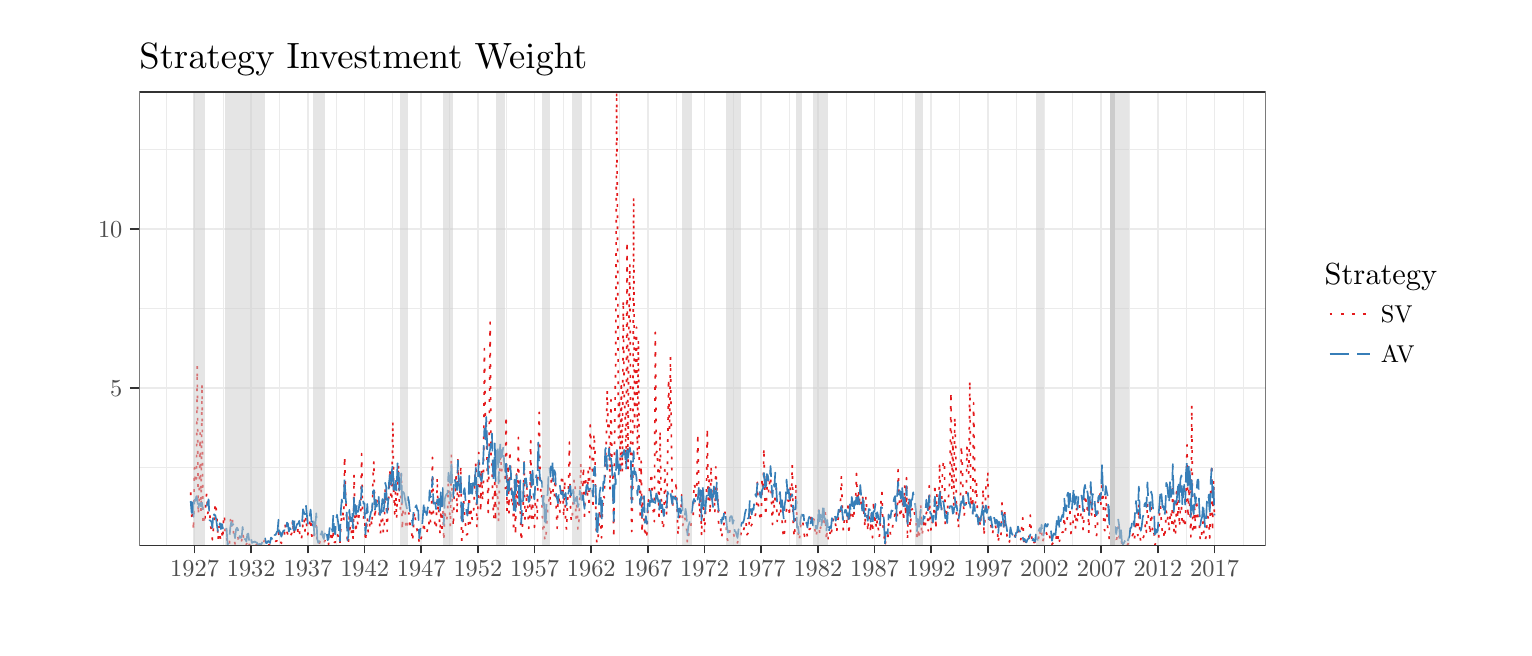
\begin{tikzpicture}[x=1.25pt,y=1pt]
\definecolor{fillColor}{RGB}{255,255,255}
\path[use as bounding box,fill=fillColor,fill opacity=0.00] (0,0) rectangle (426.79,216.81);
\begin{scope}
\path[clip] (  0.00,  0.00) rectangle (426.79,216.81);
\definecolor{drawColor}{RGB}{255,255,255}
\definecolor{fillColor}{RGB}{255,255,255}

\path[draw=drawColor,line width= 0.6pt,line join=round,line cap=round,fill=fillColor] (  0.00,  0.00) rectangle (426.79,216.81);
\end{scope}
\begin{scope}
\path[clip] ( 32.32, 29.59) rectangle (357.87,193.67);
\definecolor{fillColor}{RGB}{255,255,255}

\path[fill=fillColor] ( 32.32, 29.59) rectangle (357.87,193.67);
\definecolor{drawColor}{gray}{0.92}

\path[draw=drawColor,line width= 0.3pt,line join=round] ( 32.32, 58.07) --
	(357.87, 58.07);

\path[draw=drawColor,line width= 0.3pt,line join=round] ( 32.32,115.38) --
	(357.87,115.38);

\path[draw=drawColor,line width= 0.3pt,line join=round] ( 32.32,172.68) --
	(357.87,172.68);

\path[draw=drawColor,line width= 0.3pt,line join=round] ( 40.06, 29.59) --
	( 40.06,193.67);

\path[draw=drawColor,line width= 0.3pt,line join=round] ( 56.44, 29.59) --
	( 56.44,193.67);

\path[draw=drawColor,line width= 0.3pt,line join=round] ( 72.82, 29.59) --
	( 72.82,193.67);

\path[draw=drawColor,line width= 0.3pt,line join=round] ( 89.21, 29.59) --
	( 89.21,193.67);

\path[draw=drawColor,line width= 0.3pt,line join=round] (105.58, 29.59) --
	(105.58,193.67);

\path[draw=drawColor,line width= 0.3pt,line join=round] (121.96, 29.59) --
	(121.96,193.67);

\path[draw=drawColor,line width= 0.3pt,line join=round] (138.35, 29.59) --
	(138.35,193.67);

\path[draw=drawColor,line width= 0.3pt,line join=round] (154.73, 29.59) --
	(154.73,193.67);

\path[draw=drawColor,line width= 0.3pt,line join=round] (171.11, 29.59) --
	(171.11,193.67);

\path[draw=drawColor,line width= 0.3pt,line join=round] (187.49, 29.59) --
	(187.49,193.67);

\path[draw=drawColor,line width= 0.3pt,line join=round] (203.87, 29.59) --
	(203.87,193.67);

\path[draw=drawColor,line width= 0.3pt,line join=round] (220.25, 29.59) --
	(220.25,193.67);

\path[draw=drawColor,line width= 0.3pt,line join=round] (236.63, 29.59) --
	(236.63,193.67);

\path[draw=drawColor,line width= 0.3pt,line join=round] (253.01, 29.59) --
	(253.01,193.67);

\path[draw=drawColor,line width= 0.3pt,line join=round] (269.39, 29.59) --
	(269.39,193.67);

\path[draw=drawColor,line width= 0.3pt,line join=round] (285.77, 29.59) --
	(285.77,193.67);

\path[draw=drawColor,line width= 0.3pt,line join=round] (302.15, 29.59) --
	(302.15,193.67);

\path[draw=drawColor,line width= 0.3pt,line join=round] (318.53, 29.59) --
	(318.53,193.67);

\path[draw=drawColor,line width= 0.3pt,line join=round] (334.91, 29.59) --
	(334.91,193.67);

\path[draw=drawColor,line width= 0.3pt,line join=round] (351.30, 29.59) --
	(351.30,193.67);

\path[draw=drawColor,line width= 0.6pt,line join=round] ( 32.32, 86.72) --
	(357.87, 86.72);

\path[draw=drawColor,line width= 0.6pt,line join=round] ( 32.32,144.03) --
	(357.87,144.03);

\path[draw=drawColor,line width= 0.6pt,line join=round] ( 48.25, 29.59) --
	( 48.25,193.67);

\path[draw=drawColor,line width= 0.6pt,line join=round] ( 64.63, 29.59) --
	( 64.63,193.67);

\path[draw=drawColor,line width= 0.6pt,line join=round] ( 81.02, 29.59) --
	( 81.02,193.67);

\path[draw=drawColor,line width= 0.6pt,line join=round] ( 97.40, 29.59) --
	( 97.40,193.67);

\path[draw=drawColor,line width= 0.6pt,line join=round] (113.77, 29.59) --
	(113.77,193.67);

\path[draw=drawColor,line width= 0.6pt,line join=round] (130.15, 29.59) --
	(130.15,193.67);

\path[draw=drawColor,line width= 0.6pt,line join=round] (146.54, 29.59) --
	(146.54,193.67);

\path[draw=drawColor,line width= 0.6pt,line join=round] (162.92, 29.59) --
	(162.92,193.67);

\path[draw=drawColor,line width= 0.6pt,line join=round] (179.30, 29.59) --
	(179.30,193.67);

\path[draw=drawColor,line width= 0.6pt,line join=round] (195.68, 29.59) --
	(195.68,193.67);

\path[draw=drawColor,line width= 0.6pt,line join=round] (212.06, 29.59) --
	(212.06,193.67);

\path[draw=drawColor,line width= 0.6pt,line join=round] (228.44, 29.59) --
	(228.44,193.67);

\path[draw=drawColor,line width= 0.6pt,line join=round] (244.82, 29.59) --
	(244.82,193.67);

\path[draw=drawColor,line width= 0.6pt,line join=round] (261.20, 29.59) --
	(261.20,193.67);

\path[draw=drawColor,line width= 0.6pt,line join=round] (277.59, 29.59) --
	(277.59,193.67);

\path[draw=drawColor,line width= 0.6pt,line join=round] (293.96, 29.59) --
	(293.96,193.67);

\path[draw=drawColor,line width= 0.6pt,line join=round] (310.34, 29.59) --
	(310.34,193.67);

\path[draw=drawColor,line width= 0.6pt,line join=round] (326.72, 29.59) --
	(326.72,193.67);

\path[draw=drawColor,line width= 0.6pt,line join=round] (343.11, 29.59) --
	(343.11,193.67);
\definecolor{drawColor}{RGB}{228,26,28}

\path[draw=drawColor,line width= 0.6pt,dash pattern=on 1pt off 3pt ,line join=round] ( 47.12, 48.89) --
	( 47.40, 40.23) --
	( 47.67, 46.35) --
	( 47.95, 35.12) --
	( 48.22, 57.83) --
	( 48.49, 52.69) --
	( 48.77, 52.09) --
	( 49.02, 94.67) --
	( 49.30, 40.74) --
	( 49.57, 45.84) --
	( 49.85, 70.42) --
	( 50.12, 42.05) --
	( 50.40, 88.22) --
	( 50.67, 37.82) --
	( 50.94, 39.86) --
	( 51.22, 37.55) --
	( 51.49, 46.52) --
	( 51.77, 48.46) --
	( 52.05, 41.28) --
	( 52.31, 42.50) --
	( 52.58, 42.67) --
	( 52.85, 37.08) --
	( 53.13, 35.05) --
	( 53.40, 31.76) --
	( 53.68, 35.53) --
	( 53.96, 40.23) --
	( 54.23, 45.08) --
	( 54.50, 42.93) --
	( 54.77, 38.21) --
	( 55.05, 31.74) --
	( 55.33, 36.58) --
	( 55.58, 32.94) --
	( 55.86, 31.76) --
	( 56.13, 34.32) --
	( 56.40, 32.02) --
	( 56.67, 40.73) --
	( 56.95, 39.40) --
	( 57.23, 32.87) --
	( 57.50, 33.11) --
	( 57.78, 29.59) --
	( 58.05, 29.70) --
	( 58.32, 30.51) --
	( 58.60, 39.02) --
	( 58.85, 36.07) --
	( 59.13, 39.72) --
	( 59.40, 35.96) --
	( 59.68, 31.66) --
	( 59.95, 30.25) --
	( 60.23, 31.86) --
	( 60.50, 32.06) --
	( 60.77, 32.98) --
	( 61.05, 30.37) --
	( 61.32, 31.01) --
	( 61.60, 30.79) --
	( 61.88, 31.54) --
	( 62.13, 34.29) --
	( 62.41, 32.48) --
	( 62.67, 31.17) --
	( 62.95, 31.45) --
	( 63.22, 29.98) --
	( 63.50, 31.16) --
	( 63.78, 31.93) --
	( 64.05, 30.06) --
	( 64.32, 29.70) --
	( 64.59, 30.46) --
	( 64.87, 29.98) --
	( 65.15, 30.09) --
	( 65.41, 29.87) --
	( 65.69, 30.43) --
	( 65.96, 30.20) --
	( 66.24, 30.09) --
	( 66.50, 29.84) --
	( 66.78, 30.22) --
	( 67.06, 29.79) --
	( 67.33, 29.69) --
	( 67.61, 29.76) --
	( 67.88, 29.94) --
	( 68.15, 30.72) --
	( 68.43, 31.58) --
	( 68.68, 30.36) --
	( 68.96, 29.71) --
	( 69.23, 29.89) --
	( 69.51, 30.39) --
	( 69.78, 29.94) --
	( 70.06, 29.72) --
	( 70.33, 30.37) --
	( 70.60, 30.24) --
	( 70.88, 29.85) --
	( 71.15, 30.67) --
	( 71.43, 31.26) --
	( 71.71, 31.20) --
	( 71.96, 31.40) --
	( 72.24, 31.24) --
	( 72.51, 34.34) --
	( 72.78, 30.97) --
	( 73.05, 31.14) --
	( 73.33, 30.50) --
	( 73.61, 31.24) --
	( 73.88, 31.94) --
	( 74.16, 32.54) --
	( 74.42, 37.40) --
	( 74.70, 33.82) --
	( 74.98, 34.47) --
	( 75.23, 33.57) --
	( 75.51, 32.81) --
	( 75.78, 34.06) --
	( 76.06, 33.40) --
	( 76.33, 34.06) --
	( 76.60, 39.03) --
	( 76.88, 33.50) --
	( 77.15, 35.02) --
	( 77.43, 33.41) --
	( 77.70, 33.52) --
	( 77.98, 34.21) --
	( 78.25, 36.70) --
	( 78.51, 35.38) --
	( 78.79, 32.01) --
	( 79.06, 31.64) --
	( 79.34, 33.60) --
	( 79.61, 38.68) --
	( 79.89, 39.63) --
	( 80.17, 34.88) --
	( 80.43, 40.16) --
	( 80.71, 36.00) --
	( 80.98, 33.54) --
	( 81.26, 36.66) --
	( 81.54, 37.95) --
	( 81.79, 39.56) --
	( 82.07, 33.77) --
	( 82.34, 31.49) --
	( 82.61, 33.07) --
	( 82.88, 33.60) --
	( 83.16, 35.11) --
	( 83.44, 36.93) --
	( 83.71, 30.14) --
	( 83.99, 29.77) --
	( 84.26, 30.02) --
	( 84.53, 31.27) --
	( 84.81, 30.81) --
	( 85.06, 31.13) --
	( 85.34, 30.44) --
	( 85.61, 30.13) --
	( 85.89, 31.54) --
	( 86.16, 30.74) --
	( 86.43, 31.38) --
	( 86.71, 31.69) --
	( 86.98, 30.12) --
	( 87.26, 33.02) --
	( 87.53, 32.49) --
	( 87.81, 34.95) --
	( 88.09, 31.23) --
	( 88.34, 34.03) --
	( 88.61, 30.89) --
	( 88.88, 30.78) --
	( 89.16, 33.84) --
	( 89.43, 33.74) --
	( 89.71, 33.22) --
	( 89.99, 31.29) --
	( 90.26, 30.24) --
	( 90.53, 36.37) --
	( 90.80, 41.47) --
	( 91.08, 42.03) --
	( 91.36, 38.20) --
	( 91.62, 61.86) --
	( 91.90, 47.39) --
	( 92.17, 41.18) --
	( 92.44, 30.02) --
	( 92.71, 30.74) --
	( 92.99, 41.72) --
	( 93.27, 33.39) --
	( 93.54, 33.56) --
	( 93.82, 39.60) --
	( 94.09, 31.64) --
	( 94.36, 55.39) --
	( 94.64, 38.33) --
	( 94.89, 34.21) --
	( 95.17, 41.08) --
	( 95.44, 37.03) --
	( 95.72, 39.96) --
	( 95.99, 42.14) --
	( 96.27, 41.36) --
	( 96.54, 62.88) --
	( 96.81, 42.73) --
	( 97.09, 39.57) --
	( 97.36, 42.57) --
	( 97.64, 31.10) --
	( 97.92, 35.24) --
	( 98.17, 39.93) --
	( 98.45, 34.13) --
	( 98.71, 34.25) --
	( 98.99, 39.41) --
	( 99.26, 38.75) --
	( 99.54, 36.72) --
	( 99.82, 54.23) --
	(100.09, 60.29) --
	(100.36, 39.40) --
	(100.63, 43.76) --
	(100.91, 45.76) --
	(101.19, 47.40) --
	(101.44, 45.63) --
	(101.72, 38.05) --
	(101.99, 33.86) --
	(102.27, 39.98) --
	(102.54, 40.71) --
	(102.81, 34.21) --
	(103.09, 36.66) --
	(103.36, 50.06) --
	(103.64, 45.25) --
	(103.91, 34.80) --
	(104.19, 42.70) --
	(104.46, 49.28) --
	(104.72, 57.44) --
	(105.00, 47.13) --
	(105.27, 45.79) --
	(105.55, 74.55) --
	(105.82, 49.70) --
	(106.10, 41.10) --
	(106.37, 51.48) --
	(106.64, 39.29) --
	(106.92, 49.20) --
	(107.19, 59.10) --
	(107.47, 44.28) --
	(107.75, 42.60) --
	(108.00, 55.98) --
	(108.28, 35.28) --
	(108.54, 42.88) --
	(108.82, 43.48) --
	(109.09, 42.70) --
	(109.37, 35.85) --
	(109.65, 35.46) --
	(109.92, 39.49) --
	(110.20, 41.44) --
	(110.46, 38.01) --
	(110.74, 35.64) --
	(111.02, 34.15) --
	(111.27, 31.19) --
	(111.55, 36.48) --
	(111.82, 42.05) --
	(112.10, 38.99) --
	(112.37, 36.48) --
	(112.64, 34.93) --
	(112.92, 34.54) --
	(113.19, 30.07) --
	(113.47, 31.19) --
	(113.74, 32.27) --
	(114.02, 33.69) --
	(114.29, 35.04) --
	(114.55, 38.25) --
	(114.82, 34.07) --
	(115.09, 34.33) --
	(115.37, 34.04) --
	(115.64, 36.16) --
	(115.92, 35.61) --
	(116.20, 42.17) --
	(116.46, 37.93) --
	(116.74, 41.27) --
	(117.01, 61.55) --
	(117.29, 41.45) --
	(117.57, 39.94) --
	(117.83, 35.59) --
	(118.11, 35.79) --
	(118.38, 54.19) --
	(118.65, 40.72) --
	(118.92, 42.41) --
	(119.20, 33.71) --
	(119.48, 42.49) --
	(119.75, 34.22) --
	(120.03, 46.93) --
	(120.29, 31.32) --
	(120.57, 42.84) --
	(120.85, 38.20) --
	(121.10, 39.06) --
	(121.38, 40.66) --
	(121.65, 54.36) --
	(121.93, 42.78) --
	(122.20, 36.48) --
	(122.47, 62.91) --
	(122.75, 42.34) --
	(123.02, 36.49) --
	(123.30, 47.94) --
	(123.57, 47.41) --
	(123.85, 56.02) --
	(124.12, 41.34) --
	(124.38, 62.05) --
	(124.65, 46.47) --
	(124.92, 47.50) --
	(125.20, 58.53) --
	(125.47, 31.33) --
	(125.75, 32.68) --
	(126.03, 45.98) --
	(126.30, 40.75) --
	(126.57, 37.15) --
	(126.84, 33.58) --
	(127.12, 33.69) --
	(127.40, 36.95) --
	(127.65, 49.57) --
	(127.93, 37.65) --
	(128.20, 42.59) --
	(128.48, 39.17) --
	(128.74, 39.56) --
	(129.02, 44.23) --
	(129.30, 54.25) --
	(129.57, 59.78) --
	(129.85, 36.09) --
	(130.12, 41.76) --
	(130.39, 63.28) --
	(130.67, 55.50) --
	(130.93, 41.69) --
	(131.21, 57.56) --
	(131.48, 45.79) --
	(131.76, 52.93) --
	(132.03,100.84) --
	(132.31, 74.98) --
	(132.58, 73.05) --
	(132.85, 56.56) --
	(133.13, 41.58) --
	(133.40, 65.21) --
	(133.68,110.41) --
	(133.96, 61.65) --
	(134.21, 61.31) --
	(134.48, 44.85) --
	(134.75, 39.48) --
	(135.03, 52.51) --
	(135.30, 38.50) --
	(135.58, 51.50) --
	(135.86, 47.29) --
	(136.13, 38.02) --
	(136.40, 53.31) --
	(136.67, 66.16) --
	(136.95, 56.12) --
	(137.23, 58.48) --
	(137.48, 59.63) --
	(137.76, 61.49) --
	(138.03, 50.21) --
	(138.31, 76.47) --
	(138.57, 41.99) --
	(138.85, 59.04) --
	(139.13, 41.28) --
	(139.40, 63.93) --
	(139.68, 53.84) --
	(139.95, 44.30) --
	(140.23, 45.59) --
	(140.50, 34.72) --
	(140.75, 51.84) --
	(141.03, 33.41) --
	(141.30, 55.55) --
	(141.58, 44.09) --
	(141.85, 68.74) --
	(142.13, 41.85) --
	(142.40, 42.28) --
	(142.67, 31.23) --
	(142.95, 34.57) --
	(143.22, 42.73) --
	(143.50, 60.22) --
	(143.78, 38.96) --
	(144.04, 41.00) --
	(144.32, 50.99) --
	(144.58, 42.52) --
	(144.86, 35.86) --
	(145.13, 40.57) --
	(145.41, 67.58) --
	(145.69, 39.56) --
	(145.96, 45.90) --
	(146.23, 36.76) --
	(146.50, 36.27) --
	(146.78, 46.07) --
	(147.06, 45.26) --
	(147.31, 38.81) --
	(147.59, 61.75) --
	(147.86, 77.84) --
	(148.14, 54.92) --
	(148.41, 46.64) --
	(148.68, 47.73) --
	(148.96, 34.36) --
	(149.23, 36.61) --
	(149.51, 31.33) --
	(149.78, 32.21) --
	(150.06, 37.62) --
	(150.33, 43.32) --
	(150.59, 43.79) --
	(150.86, 50.40) --
	(151.13, 43.85) --
	(151.41, 55.18) --
	(151.68, 54.28) --
	(151.96, 47.32) --
	(152.24, 46.77) --
	(152.50, 55.73) --
	(152.78, 42.84) --
	(153.05, 35.84) --
	(153.33, 47.05) --
	(153.61, 46.46) --
	(153.86, 41.72) --
	(154.14, 49.20) --
	(154.41, 55.29) --
	(154.68, 52.79) --
	(154.95, 39.91) --
	(155.23, 53.22) --
	(155.51, 38.55) --
	(155.78, 35.31) --
	(156.06, 45.60) --
	(156.33, 50.92) --
	(156.60, 67.07) --
	(156.88, 44.83) --
	(157.14, 38.25) --
	(157.42, 39.51) --
	(157.69, 45.76) --
	(157.97, 53.74) --
	(158.24, 51.62) --
	(158.51, 39.22) --
	(158.79, 45.92) --
	(159.06, 35.30) --
	(159.34, 38.34) --
	(159.61, 46.62) --
	(159.89, 59.55) --
	(160.16, 48.11) --
	(160.42, 49.51) --
	(160.69, 58.12) --
	(160.96, 38.62) --
	(161.24, 54.74) --
	(161.51, 48.95) --
	(161.79, 46.54) --
	(162.07, 56.89) --
	(162.34, 41.60) --
	(162.61, 73.27) --
	(162.88, 65.85) --
	(163.16, 61.66) --
	(163.44, 42.90) --
	(163.69, 70.10) --
	(163.97, 64.91) --
	(164.24, 40.67) --
	(164.51, 30.33) --
	(164.78, 31.02) --
	(165.06, 35.27) --
	(165.34, 42.75) --
	(165.61, 39.16) --
	(165.89, 32.44) --
	(166.16, 41.85) --
	(166.43, 47.79) --
	(166.71, 46.92) --
	(166.96, 58.93) --
	(167.24, 65.79) --
	(167.51, 85.85) --
	(167.79, 71.92) --
	(168.06, 73.86) --
	(168.34, 49.70) --
	(168.61, 82.36) --
	(168.88, 61.68) --
	(169.16, 54.56) --
	(169.43, 32.53) --
	(169.71, 74.21) --
	(169.99, 96.23) --
	(170.25,193.67) --
	(170.52,141.45) --
	(170.79, 68.56) --
	(171.07, 82.79) --
	(171.34, 55.88) --
	(171.62, 88.94) --
	(171.90, 56.06) --
	(172.17,118.36) --
	(172.44, 83.73) --
	(172.71, 77.35) --
	(172.99, 58.46) --
	(173.27,139.51) --
	(173.52, 57.07) --
	(173.80,111.22) --
	(174.07,131.56) --
	(174.35, 61.86) --
	(174.61, 34.72) --
	(174.89, 49.02) --
	(175.17,155.71) --
	(175.44, 70.66) --
	(175.72, 92.87) --
	(175.99,108.55) --
	(176.26, 61.82) --
	(176.54,104.10) --
	(176.79, 61.04) --
	(177.07, 39.05) --
	(177.34, 60.42) --
	(177.62, 34.31) --
	(177.89, 47.81) --
	(178.17, 39.44) --
	(178.44, 32.72) --
	(178.71, 35.77) --
	(178.99, 33.49) --
	(179.26, 42.25) --
	(179.54, 47.04) --
	(179.82, 51.21) --
	(180.07, 52.80) --
	(180.35, 55.93) --
	(180.62, 42.73) --
	(180.89, 42.26) --
	(181.16, 38.30) --
	(181.44,106.74) --
	(181.72, 63.23) --
	(181.99, 64.05) --
	(182.27, 54.43) --
	(182.53, 38.62) --
	(182.81, 71.25) --
	(183.09, 50.13) --
	(183.35, 40.38) --
	(183.63, 35.45) --
	(183.90, 37.57) --
	(184.18, 57.11) --
	(184.45, 46.31) --
	(184.72, 40.50) --
	(185.00, 62.51) --
	(185.27, 89.98) --
	(185.55, 71.54) --
	(185.82, 98.01) --
	(186.10, 67.23) --
	(186.37, 42.94) --
	(186.62, 46.72) --
	(186.90, 46.60) --
	(187.17, 46.26) --
	(187.45, 52.84) --
	(187.72, 43.23) --
	(188.00, 33.29) --
	(188.28, 39.29) --
	(188.54, 40.23) --
	(188.82, 42.20) --
	(189.09, 48.04) --
	(189.37, 36.62) --
	(189.65, 40.14) --
	(189.90, 39.79) --
	(190.18, 38.68) --
	(190.45, 36.07) --
	(190.72, 30.48) --
	(190.99, 32.86) --
	(191.27, 34.59) --
	(191.55, 34.68) --
	(191.82, 38.03) --
	(192.10, 38.78) --
	(192.37, 40.31) --
	(192.64, 52.11) --
	(192.92, 50.77) --
	(193.17, 47.45) --
	(193.45, 51.84) --
	(193.72, 70.09) --
	(194.00, 49.36) --
	(194.27, 39.46) --
	(194.54, 48.24) --
	(194.82, 33.16) --
	(195.09, 47.67) --
	(195.37, 44.85) --
	(195.64, 34.31) --
	(195.92, 41.00) --
	(196.20, 47.96) --
	(196.46, 72.08) --
	(196.73, 45.83) --
	(197.00, 53.72) --
	(197.28, 41.12) --
	(197.55, 58.56) --
	(197.83, 45.94) --
	(198.11, 47.88) --
	(198.37, 49.58) --
	(198.65, 41.43) --
	(198.92, 58.13) --
	(199.20, 49.71) --
	(199.48, 47.52) --
	(199.73, 37.91) --
	(200.01, 35.85) --
	(200.28, 36.46) --
	(200.55, 32.49) --
	(200.82, 34.23) --
	(201.10, 35.22) --
	(201.38, 38.96) --
	(201.65, 42.61) --
	(201.93, 36.96) --
	(202.20, 32.05) --
	(202.47, 31.35) --
	(202.75, 32.62) --
	(203.00, 35.27) --
	(203.28, 35.90) --
	(203.55, 35.48) --
	(203.83, 34.60) --
	(204.10, 33.77) --
	(204.38, 31.51) --
	(204.65, 31.85) --
	(204.92, 30.86) --
	(205.20, 30.66) --
	(205.47, 32.46) --
	(205.75, 32.16) --
	(206.03, 32.57) --
	(206.28, 34.83) --
	(206.56, 33.85) --
	(206.82, 34.67) --
	(207.10, 35.98) --
	(207.37, 38.05) --
	(207.65, 38.42) --
	(207.93, 33.58) --
	(208.20, 34.04) --
	(208.47, 34.92) --
	(208.74, 42.77) --
	(209.02, 36.50) --
	(209.30, 37.21) --
	(209.56, 37.76) --
	(209.84, 38.66) --
	(210.11, 39.41) --
	(210.39, 40.88) --
	(210.65, 42.27) --
	(210.93, 52.53) --
	(211.21, 44.29) --
	(211.48, 43.25) --
	(211.76, 38.49) --
	(212.03, 39.22) --
	(212.30, 54.00) --
	(212.58, 49.52) --
	(212.83, 64.94) --
	(213.11, 46.87) --
	(213.38, 40.38) --
	(213.66, 48.65) --
	(213.93, 55.89) --
	(214.21, 48.85) --
	(214.48, 52.31) --
	(214.75, 54.65) --
	(215.03, 45.44) --
	(215.30, 37.25) --
	(215.58, 46.65) --
	(215.86, 43.18) --
	(216.11, 48.00) --
	(216.39, 50.35) --
	(216.65, 38.36) --
	(216.93, 41.34) --
	(217.20, 40.70) --
	(217.48, 45.64) --
	(217.76, 40.89) --
	(218.03, 39.59) --
	(218.31, 34.71) --
	(218.57, 32.37) --
	(218.85, 35.36) --
	(219.13, 40.34) --
	(219.38, 42.77) --
	(219.66, 46.02) --
	(219.93, 45.97) --
	(220.21, 40.10) --
	(220.48, 51.14) --
	(220.75, 43.83) --
	(221.03, 58.93) --
	(221.30, 37.64) --
	(221.58, 32.67) --
	(221.85, 36.38) --
	(222.13, 52.15) --
	(222.40, 35.10) --
	(222.66, 35.38) --
	(222.94, 31.40) --
	(223.21, 33.02) --
	(223.49, 37.28) --
	(223.76, 37.79) --
	(224.04, 39.04) --
	(224.31, 35.15) --
	(224.58, 33.05) --
	(224.86, 33.87) --
	(225.13, 34.96) --
	(225.41, 32.73) --
	(225.69, 35.36) --
	(225.94, 35.60) --
	(226.22, 35.73) --
	(226.49, 41.21) --
	(226.76, 40.90) --
	(227.03, 39.43) --
	(227.31, 39.11) --
	(227.59, 35.26) --
	(227.86, 32.72) --
	(228.14, 34.65) --
	(228.40, 37.16) --
	(228.68, 42.45) --
	(228.96, 33.46) --
	(229.21, 36.33) --
	(229.49, 35.48) --
	(229.76, 39.76) --
	(230.04, 42.29) --
	(230.31, 36.61) --
	(230.58, 42.10) --
	(230.86, 31.50) --
	(231.13, 35.05) --
	(231.41, 31.51) --
	(231.68, 31.59) --
	(231.96, 34.41) --
	(232.23, 32.75) --
	(232.49, 35.98) --
	(232.76, 38.12) --
	(233.03, 40.01) --
	(233.31, 38.51) --
	(233.58, 37.08) --
	(233.86, 34.33) --
	(234.14, 38.12) --
	(234.41, 40.46) --
	(234.68, 39.93) --
	(234.95, 44.49) --
	(235.23, 54.95) --
	(235.51, 42.60) --
	(235.77, 35.03) --
	(236.05, 38.51) --
	(236.32, 41.85) --
	(236.59, 42.32) --
	(236.86, 37.45) --
	(237.14, 43.99) --
	(237.42, 33.62) --
	(237.69, 44.20) --
	(237.97, 39.81) --
	(238.24, 41.69) --
	(238.51, 40.71) --
	(238.79, 38.96) --
	(239.04, 45.34) --
	(239.32, 44.82) --
	(239.59, 55.76) --
	(239.87, 45.40) --
	(240.14, 49.97) --
	(240.42, 45.33) --
	(240.69, 49.57) --
	(240.96, 43.93) --
	(241.24, 45.24) --
	(241.51, 48.19) --
	(241.79, 40.29) --
	(242.07, 36.20) --
	(242.32, 47.46) --
	(242.59, 42.31) --
	(242.86, 34.68) --
	(243.14, 40.43) --
	(243.41, 38.93) --
	(243.69, 34.25) --
	(243.97, 42.75) --
	(244.24, 32.47) --
	(244.51, 45.88) --
	(244.78, 37.33) --
	(245.06, 40.05) --
	(245.34, 35.64) --
	(245.59, 38.93) --
	(245.87, 36.15) --
	(246.14, 32.49) --
	(246.42, 34.88) --
	(246.68, 45.78) --
	(246.96, 48.88) --
	(247.24, 36.93) --
	(247.51, 34.96) --
	(247.79, 29.60) --
	(248.06, 31.26) --
	(248.34, 31.38) --
	(248.61, 30.87) --
	(248.87, 37.38) --
	(249.15, 37.57) --
	(249.42, 33.43) --
	(249.70, 35.04) --
	(249.97, 36.07) --
	(250.25, 37.98) --
	(250.52, 39.12) --
	(250.79, 42.76) --
	(251.07, 38.94) --
	(251.34, 39.14) --
	(251.62, 57.10) --
	(251.90, 48.29) --
	(252.15, 41.57) --
	(252.43, 39.71) --
	(252.69, 49.26) --
	(252.97, 44.27) --
	(253.24, 38.44) --
	(253.52, 51.55) --
	(253.80, 40.38) --
	(254.07, 54.19) --
	(254.34, 31.75) --
	(254.61, 45.31) --
	(254.89, 42.44) --
	(255.17, 34.30) --
	(255.42, 42.41) --
	(255.70, 42.92) --
	(255.97, 42.07) --
	(256.25, 43.11) --
	(256.52, 39.31) --
	(256.79, 38.82) --
	(257.07, 31.29) --
	(257.34, 35.75) --
	(257.62, 32.04) --
	(257.89, 34.84) --
	(258.17, 44.70) --
	(258.44, 33.11) --
	(258.70, 34.80) --
	(258.97, 38.01) --
	(259.24, 35.50) --
	(259.52, 37.32) --
	(259.79, 41.56) --
	(260.07, 42.15) --
	(260.35, 34.99) --
	(260.61, 51.29) --
	(260.89, 39.54) --
	(261.16, 34.93) --
	(261.44, 36.99) --
	(261.72, 41.21) --
	(261.98, 41.47) --
	(262.26, 51.93) --
	(262.53, 35.48) --
	(262.80, 48.45) --
	(263.07, 43.24) --
	(263.35, 43.26) --
	(263.63, 59.65) --
	(263.90, 42.23) --
	(264.18, 42.09) --
	(264.44, 56.06) --
	(264.72, 60.09) --
	(265.00, 60.35) --
	(265.25, 37.12) --
	(265.53, 42.99) --
	(265.80, 40.63) --
	(266.08, 45.69) --
	(266.35, 49.51) --
	(266.62, 54.70) --
	(266.90, 85.12) --
	(267.17, 49.99) --
	(267.45, 68.95) --
	(267.72, 43.77) --
	(268.00, 76.12) --
	(268.27, 65.10) --
	(268.53, 39.99) --
	(268.80, 40.75) --
	(269.07, 35.86) --
	(269.35, 43.60) --
	(269.62, 43.46) --
	(269.90, 65.79) --
	(270.18, 58.63) --
	(270.45, 45.81) --
	(270.72, 40.15) --
	(270.99, 44.06) --
	(271.27, 44.70) --
	(271.55, 65.65) --
	(271.80, 55.28) --
	(272.08, 56.14) --
	(272.35, 89.34) --
	(272.62, 43.99) --
	(272.89, 47.20) --
	(273.17, 41.32) --
	(273.45, 81.28) --
	(273.72, 59.46) --
	(274.00, 45.08) --
	(274.27, 52.44) --
	(274.54, 41.42) --
	(274.82, 37.52) --
	(275.08, 40.49) --
	(275.36, 36.37) --
	(275.63, 41.43) --
	(275.91, 40.48) --
	(276.18, 50.37) --
	(276.45, 33.10) --
	(276.73, 39.72) --
	(277.00, 50.85) --
	(277.28, 50.38) --
	(277.55, 56.45) --
	(277.83, 37.44) --
	(278.11, 39.99) --
	(278.36, 37.86) --
	(278.63, 35.79) --
	(278.90, 33.67) --
	(279.18, 36.14) --
	(279.45, 37.41) --
	(279.73, 37.08) --
	(280.01, 35.36) --
	(280.28, 35.75) --
	(280.55, 30.66) --
	(280.82, 33.66) --
	(281.10, 34.61) --
	(281.38, 33.64) --
	(281.63, 45.32) --
	(281.91, 41.03) --
	(282.18, 35.56) --
	(282.46, 41.80) --
	(282.72, 34.87) --
	(283.00, 34.60) --
	(283.28, 30.62) --
	(283.55, 30.53) --
	(283.83, 31.08) --
	(284.10, 35.15) --
	(284.38, 33.13) --
	(284.65, 32.82) --
	(284.90, 32.46) --
	(285.18, 32.94) --
	(285.45, 33.34) --
	(285.73, 32.99) --
	(286.00, 33.79) --
	(286.28, 35.63) --
	(286.55, 33.15) --
	(286.82, 33.41) --
	(287.10, 31.78) --
	(287.37, 36.66) --
	(287.65, 39.69) --
	(287.93, 31.12) --
	(288.19, 32.97) --
	(288.47, 30.97) --
	(288.73, 30.26) --
	(289.01, 30.84) --
	(289.28, 32.55) --
	(289.56, 32.97) --
	(289.84, 40.70) --
	(290.11, 34.62) --
	(290.38, 30.75) --
	(290.65, 31.74) --
	(290.93, 30.73) --
	(291.21, 30.96) --
	(291.46, 33.59) --
	(291.74, 30.78) --
	(292.01, 30.62) --
	(292.29, 32.89) --
	(292.56, 35.39) --
	(292.83, 32.95) --
	(293.11, 34.67) --
	(293.38, 30.81) --
	(293.66, 32.25) --
	(293.93, 34.66) --
	(294.21, 34.49) --
	(294.48, 34.23) --
	(294.73, 33.31) --
	(295.01, 34.58) --
	(295.28, 34.17) --
	(295.56, 32.08) --
	(295.83, 32.58) --
	(296.11, 30.13) --
	(296.39, 30.57) --
	(296.65, 31.00) --
	(296.93, 30.33) --
	(297.20, 31.74) --
	(297.48, 33.57) --
	(297.76, 31.56) --
	(298.01, 33.85) --
	(298.29, 31.25) --
	(298.56, 33.43) --
	(298.83, 34.67) --
	(299.10, 34.40) --
	(299.38, 34.58) --
	(299.66, 40.09) --
	(299.93, 34.71) --
	(300.21, 37.12) --
	(300.48, 39.51) --
	(300.75, 40.78) --
	(301.03, 41.30) --
	(301.29, 42.44) --
	(301.57, 33.98) --
	(301.84, 36.58) --
	(302.12, 37.11) --
	(302.39, 40.84) --
	(302.66, 41.17) --
	(302.94, 35.72) --
	(303.21, 43.03) --
	(303.49, 37.91) --
	(303.76, 43.48) --
	(304.04, 44.30) --
	(304.31, 40.29) --
	(304.57, 41.26) --
	(304.84, 42.20) --
	(305.11, 35.05) --
	(305.39, 40.71) --
	(305.66, 48.16) --
	(305.94, 45.77) --
	(306.22, 42.57) --
	(306.48, 44.92) --
	(306.76, 34.14) --
	(307.03, 46.92) --
	(307.31, 49.25) --
	(307.59, 39.93) --
	(307.84, 44.54) --
	(308.12, 45.38) --
	(308.39, 45.55) --
	(308.66, 35.84) --
	(308.93, 33.06) --
	(309.21, 34.76) --
	(309.49, 47.00) --
	(309.76, 46.26) --
	(310.04, 48.43) --
	(310.31, 43.93) --
	(310.58, 55.01) --
	(310.86, 47.97) --
	(311.11, 35.92) --
	(311.39, 35.04) --
	(311.66, 47.68) --
	(311.94, 42.46) --
	(312.21, 35.99) --
	(312.49, 33.63) --
	(312.76, 31.35) --
	(313.03, 34.79) --
	(313.31, 34.73) --
	(313.58, 31.18) --
	(313.86, 33.29) --
	(314.14, 31.63) --
	(314.40, 32.37) --
	(314.67, 30.91) --
	(314.94, 33.13) --
	(315.22, 36.45) --
	(315.49, 33.05) --
	(315.77, 31.71) --
	(316.05, 32.70) --
	(316.32, 29.85) --
	(316.59, 29.59) --
	(316.86, 29.67) --
	(317.14, 29.88) --
	(317.42, 30.17) --
	(317.67, 30.47) --
	(317.95, 29.88) --
	(318.22, 30.60) --
	(318.50, 30.77) --
	(318.76, 31.76) --
	(319.04, 31.95) --
	(319.32, 33.21) --
	(319.59, 33.90) --
	(319.87, 31.56) --
	(320.14, 33.95) --
	(320.41, 38.99) --
	(320.69, 34.29) --
	(320.94, 33.27) --
	(321.22, 44.58) --
	(321.49, 34.36) --
	(321.77, 30.54) --
	(322.04, 31.04) --
	(322.32, 32.29) --
	(322.59, 32.81) --
	(322.86, 34.19) --
	(323.14, 37.83) --
	(323.41, 34.42) --
	(323.69, 45.04) --
	(323.97, 39.35) --
	(324.22, 37.74) --
	(324.50, 33.63) --
	(324.76, 43.36) --
	(325.04, 37.57) --
	(325.31, 33.32) --
	(325.59, 34.32) --
	(325.87, 29.89) --
	(326.14, 30.80) --
	(326.42, 30.63) --
	(326.68, 30.59) --
	(326.96, 32.50) --
	(327.24, 44.17) --
	(327.50, 43.57) --
	(327.78, 36.54) --
	(328.05, 34.69) --
	(328.33, 35.79) --
	(328.59, 32.11) --
	(328.87, 35.42) --
	(329.15, 42.13) --
	(329.42, 38.68) --
	(329.70, 40.53) --
	(329.97, 34.64) --
	(330.25, 40.47) --
	(330.52, 42.25) --
	(330.77, 37.40) --
	(331.05, 53.89) --
	(331.32, 34.51) --
	(331.60, 38.86) --
	(331.87, 33.59) --
	(332.15, 50.78) --
	(332.42, 39.26) --
	(332.69, 46.32) --
	(332.97, 36.41) --
	(333.24, 44.40) --
	(333.52, 43.65) --
	(333.80, 36.83) --
	(334.05, 37.59) --
	(334.33, 40.18) --
	(334.60, 35.93) --
	(334.87, 46.93) --
	(335.14, 66.06) --
	(335.42, 39.75) --
	(335.70, 50.86) --
	(335.97, 42.65) --
	(336.25, 32.76) --
	(336.52, 80.37) --
	(336.79, 34.17) --
	(337.07, 34.04) --
	(337.32, 43.59) --
	(337.60, 35.65) --
	(337.87, 46.33) --
	(338.15, 41.82) --
	(338.42, 38.67) --
	(338.69, 37.91) --
	(338.97, 31.30) --
	(339.24, 31.90) --
	(339.52, 35.99) --
	(339.79, 38.28) --
	(340.07, 33.05) --
	(340.35, 31.59) --
	(340.61, 32.68) --
	(340.88, 36.66) --
	(341.15, 40.18) --
	(341.43, 38.83) --
	(341.70, 32.42) --
	(341.98, 49.51) --
	(342.26, 59.00) --
	(342.52, 34.77) --
	(342.80, 53.33) --
	(343.07, 40.24);
\definecolor{drawColor}{RGB}{55,126,184}

\path[draw=drawColor,line width= 0.6pt,dash pattern=on 7pt off 3pt ,line join=round] ( 47.12, 45.75) --
	( 47.40, 41.45) --
	( 47.67, 46.33) --
	( 47.95, 40.05) --
	( 48.22, 46.22) --
	( 48.49, 45.82) --
	( 48.77, 47.51) --
	( 49.02, 46.51) --
	( 49.30, 42.41) --
	( 49.57, 44.81) --
	( 49.85, 45.01) --
	( 50.12, 43.84) --
	( 50.40, 45.17) --
	( 50.67, 42.18) --
	( 50.94, 42.89) --
	( 51.22, 42.84) --
	( 51.49, 43.95) --
	( 51.77, 44.03) --
	( 52.05, 45.21) --
	( 52.31, 46.38) --
	( 52.58, 38.83) --
	( 52.85, 38.70) --
	( 53.13, 38.22) --
	( 53.40, 36.05) --
	( 53.68, 41.93) --
	( 53.96, 40.54) --
	( 54.23, 40.69) --
	( 54.50, 39.02) --
	( 54.77, 36.54) --
	( 55.05, 34.45) --
	( 55.33, 36.35) --
	( 55.58, 37.77) --
	( 55.86, 35.61) --
	( 56.13, 37.52) --
	( 56.40, 35.83) --
	( 56.67, 37.04) --
	( 56.95, 37.13) --
	( 57.23, 35.37) --
	( 57.50, 35.81) --
	( 57.78, 30.06) --
	( 58.05, 30.51) --
	( 58.32, 32.29) --
	( 58.60, 36.44) --
	( 58.85, 38.21) --
	( 59.13, 36.88) --
	( 59.40, 37.43) --
	( 59.68, 34.36) --
	( 59.95, 32.34) --
	( 60.23, 35.49) --
	( 60.50, 36.14) --
	( 60.77, 35.56) --
	( 61.05, 32.10) --
	( 61.32, 33.12) --
	( 61.60, 32.44) --
	( 61.88, 32.88) --
	( 62.13, 36.40) --
	( 62.41, 33.87) --
	( 62.67, 32.15) --
	( 62.95, 31.85) --
	( 63.22, 31.14) --
	( 63.50, 33.78) --
	( 63.78, 34.00) --
	( 64.05, 31.16) --
	( 64.32, 30.33) --
	( 64.59, 32.01) --
	( 64.87, 30.61) --
	( 65.15, 30.95) --
	( 65.41, 30.90) --
	( 65.69, 31.18) --
	( 65.96, 30.83) --
	( 66.24, 30.76) --
	( 66.50, 30.29) --
	( 66.78, 29.78) --
	( 67.06, 30.31) --
	( 67.33, 29.97) --
	( 67.61, 30.23) --
	( 67.88, 31.15) --
	( 68.15, 31.13) --
	( 68.43, 33.02) --
	( 68.68, 31.98) --
	( 68.96, 30.49) --
	( 69.23, 30.74) --
	( 69.51, 31.32) --
	( 69.78, 31.08) --
	( 70.06, 30.60) --
	( 70.33, 32.55) --
	( 70.60, 32.26) --
	( 70.88, 31.10) --
	( 71.15, 32.68) --
	( 71.43, 33.56) --
	( 71.71, 33.53) --
	( 71.96, 34.45) --
	( 72.24, 34.92) --
	( 72.51, 39.02) --
	( 72.78, 33.90) --
	( 73.05, 34.53) --
	( 73.33, 32.88) --
	( 73.61, 33.90) --
	( 73.88, 34.99) --
	( 74.16, 34.94) --
	( 74.42, 36.93) --
	( 74.70, 35.92) --
	( 74.98, 37.97) --
	( 75.23, 37.55) --
	( 75.51, 34.70) --
	( 75.78, 36.02) --
	( 76.06, 35.61) --
	( 76.33, 37.09) --
	( 76.60, 38.63) --
	( 76.88, 35.19) --
	( 77.15, 39.04) --
	( 77.43, 35.33) --
	( 77.70, 36.89) --
	( 77.98, 37.60) --
	( 78.25, 37.61) --
	( 78.51, 38.62) --
	( 78.79, 36.04) --
	( 79.06, 36.09) --
	( 79.34, 38.37) --
	( 79.61, 42.77) --
	( 79.89, 41.58) --
	( 80.17, 40.93) --
	( 80.43, 44.31) --
	( 80.71, 40.82) --
	( 80.98, 37.52) --
	( 81.26, 40.56) --
	( 81.54, 40.47) --
	( 81.79, 42.68) --
	( 82.07, 37.97) --
	( 82.34, 35.89) --
	( 82.61, 38.43) --
	( 82.88, 33.18) --
	( 83.16, 37.20) --
	( 83.44, 41.34) --
	( 83.71, 32.09) --
	( 83.99, 30.63) --
	( 84.26, 31.15) --
	( 84.53, 34.26) --
	( 84.81, 33.58) --
	( 85.06, 34.87) --
	( 85.34, 32.90) --
	( 85.61, 32.04) --
	( 85.89, 34.32) --
	( 86.16, 33.36) --
	( 86.43, 34.55) --
	( 86.71, 31.62) --
	( 86.98, 32.06) --
	( 87.26, 35.69) --
	( 87.53, 37.38) --
	( 87.81, 36.96) --
	( 88.09, 34.71) --
	( 88.34, 40.73) --
	( 88.61, 35.05) --
	( 88.88, 33.74) --
	( 89.16, 39.11) --
	( 89.43, 40.79) --
	( 89.71, 38.36) --
	( 89.99, 35.39) --
	( 90.26, 31.27) --
	( 90.53, 42.38) --
	( 90.80, 46.32) --
	( 91.08, 44.36) --
	( 91.36, 45.67) --
	( 91.62, 54.14) --
	( 91.90, 47.00) --
	( 92.17, 43.75) --
	( 92.44, 31.59) --
	( 92.71, 33.26) --
	( 92.99, 42.56) --
	( 93.27, 38.48) --
	( 93.54, 38.64) --
	( 93.82, 42.15) --
	( 94.09, 35.75) --
	( 94.36, 47.40) --
	( 94.64, 43.47) --
	( 94.89, 40.98) --
	( 95.17, 44.84) --
	( 95.44, 41.75) --
	( 95.72, 42.86) --
	( 95.99, 45.97) --
	( 96.27, 43.70) --
	( 96.54, 51.09) --
	( 96.81, 47.41) --
	( 97.09, 44.80) --
	( 97.36, 44.97) --
	( 97.64, 33.71) --
	( 97.92, 38.20) --
	( 98.17, 44.72) --
	( 98.45, 38.85) --
	( 98.71, 38.49) --
	( 98.99, 40.29) --
	( 99.26, 41.90) --
	( 99.54, 42.29) --
	( 99.82, 49.18) --
	(100.09, 49.71) --
	(100.36, 41.91) --
	(100.63, 46.14) --
	(100.91, 43.79) --
	(101.19, 46.71) --
	(101.44, 47.58) --
	(101.72, 42.39) --
	(101.99, 39.44) --
	(102.27, 42.07) --
	(102.54, 46.50) --
	(102.81, 41.77) --
	(103.09, 43.98) --
	(103.36, 52.36) --
	(103.64, 50.88) --
	(103.91, 41.46) --
	(104.19, 45.23) --
	(104.46, 52.41) --
	(104.72, 55.20) --
	(105.00, 50.95) --
	(105.27, 56.56) --
	(105.55, 58.99) --
	(105.82, 48.15) --
	(106.10, 48.47) --
	(106.37, 53.02) --
	(106.64, 49.60) --
	(106.92, 59.39) --
	(107.19, 58.81) --
	(107.47, 48.75) --
	(107.75, 48.04) --
	(108.00, 55.70) --
	(108.28, 45.03) --
	(108.54, 49.06) --
	(108.82, 48.52) --
	(109.09, 46.36) --
	(109.37, 44.57) --
	(109.65, 42.84) --
	(109.92, 47.29) --
	(110.20, 45.65) --
	(110.46, 42.38) --
	(110.74, 41.48) --
	(111.02, 39.79) --
	(111.27, 36.88) --
	(111.55, 42.29) --
	(111.82, 44.23) --
	(112.10, 43.51) --
	(112.37, 44.22) --
	(112.64, 42.45) --
	(112.92, 42.40) --
	(113.19, 32.34) --
	(113.47, 35.18) --
	(113.74, 37.38) --
	(114.02, 36.66) --
	(114.29, 41.03) --
	(114.55, 45.57) --
	(114.82, 41.74) --
	(115.09, 41.88) --
	(115.37, 40.63) --
	(115.64, 43.50) --
	(115.92, 42.88) --
	(116.20, 49.63) --
	(116.46, 47.17) --
	(116.74, 47.68) --
	(117.01, 54.53) --
	(117.29, 44.79) --
	(117.57, 45.15) --
	(117.83, 45.11) --
	(118.11, 42.36) --
	(118.38, 46.28) --
	(118.65, 44.18) --
	(118.92, 46.61) --
	(119.20, 42.28) --
	(119.48, 49.89) --
	(119.75, 43.77) --
	(120.03, 50.54) --
	(120.29, 37.14) --
	(120.57, 46.51) --
	(120.85, 47.65) --
	(121.10, 48.23) --
	(121.38, 48.53) --
	(121.65, 55.98) --
	(121.93, 54.00) --
	(122.20, 45.60) --
	(122.47, 60.57) --
	(122.75, 52.08) --
	(123.02, 47.02) --
	(123.30, 54.20) --
	(123.57, 53.03) --
	(123.85, 50.80) --
	(124.12, 49.72) --
	(124.38, 60.45) --
	(124.65, 52.07) --
	(124.92, 49.43) --
	(125.20, 54.58) --
	(125.47, 36.82) --
	(125.75, 38.65) --
	(126.03, 49.17) --
	(126.30, 50.41) --
	(126.57, 45.91) --
	(126.84, 42.16) --
	(127.12, 40.48) --
	(127.40, 43.88) --
	(127.65, 54.94) --
	(127.93, 48.52) --
	(128.20, 52.90) --
	(128.48, 48.37) --
	(128.74, 52.25) --
	(129.02, 49.77) --
	(129.30, 53.99) --
	(129.57, 57.79) --
	(129.85, 44.48) --
	(130.12, 52.04) --
	(130.39, 60.51) --
	(130.67, 54.82) --
	(130.93, 53.92) --
	(131.21, 52.80) --
	(131.48, 55.73) --
	(131.76, 62.50) --
	(132.03, 71.95) --
	(132.31, 68.01) --
	(132.58, 76.13) --
	(132.85, 64.52) --
	(133.13, 55.48) --
	(133.40, 63.20) --
	(133.68, 64.44) --
	(133.96, 67.44) --
	(134.21, 70.16) --
	(134.48, 57.16) --
	(134.75, 52.67) --
	(135.03, 66.62) --
	(135.30, 52.91) --
	(135.58, 65.91) --
	(135.86, 64.69) --
	(136.13, 52.07) --
	(136.40, 62.47) --
	(136.67, 66.95) --
	(136.95, 61.39) --
	(137.23, 62.92) --
	(137.48, 65.30) --
	(137.76, 59.08) --
	(138.03, 56.33) --
	(138.31, 59.83) --
	(138.57, 47.75) --
	(138.85, 54.07) --
	(139.13, 49.45) --
	(139.40, 58.57) --
	(139.68, 56.34) --
	(139.95, 48.10) --
	(140.23, 49.28) --
	(140.50, 42.40) --
	(140.75, 53.49) --
	(141.03, 42.16) --
	(141.30, 55.10) --
	(141.58, 52.82) --
	(141.85, 53.04) --
	(142.13, 44.21) --
	(142.40, 53.23) --
	(142.67, 37.54) --
	(142.95, 45.56) --
	(143.22, 45.87) --
	(143.50, 59.68) --
	(143.78, 52.20) --
	(144.04, 53.99) --
	(144.32, 51.10) --
	(144.58, 48.54) --
	(144.86, 45.42) --
	(145.13, 46.13) --
	(145.41, 55.34) --
	(145.69, 51.29) --
	(145.96, 56.73) --
	(146.23, 48.13) --
	(146.50, 46.36) --
	(146.78, 53.17) --
	(147.06, 55.13) --
	(147.31, 51.40) --
	(147.59, 66.91) --
	(147.86, 58.12) --
	(148.14, 53.20) --
	(148.41, 53.17) --
	(148.68, 52.70) --
	(148.96, 44.26) --
	(149.23, 48.03) --
	(149.51, 36.45) --
	(149.78, 38.23) --
	(150.06, 46.90) --
	(150.33, 48.43) --
	(150.59, 56.40) --
	(150.86, 57.64) --
	(151.13, 54.62) --
	(151.41, 60.46) --
	(151.68, 60.37) --
	(151.96, 52.46) --
	(152.24, 56.92) --
	(152.50, 55.89) --
	(152.78, 47.90) --
	(153.05, 46.48) --
	(153.33, 44.96) --
	(153.61, 50.00) --
	(153.86, 51.30) --
	(154.14, 48.48) --
	(154.41, 48.16) --
	(154.68, 49.10) --
	(154.95, 45.43) --
	(155.23, 47.50) --
	(155.51, 48.72) --
	(155.78, 44.25) --
	(156.06, 47.64) --
	(156.33, 48.67) --
	(156.60, 50.18) --
	(156.88, 51.33) --
	(157.14, 46.96) --
	(157.42, 46.51) --
	(157.69, 49.92) --
	(157.97, 45.57) --
	(158.24, 43.57) --
	(158.51, 46.47) --
	(158.79, 47.39) --
	(159.06, 43.62) --
	(159.34, 44.77) --
	(159.61, 49.47) --
	(159.89, 47.02) --
	(160.16, 46.09) --
	(160.42, 49.54) --
	(160.69, 46.15) --
	(160.96, 42.98) --
	(161.24, 47.36) --
	(161.51, 51.10) --
	(161.79, 51.67) --
	(162.07, 49.77) --
	(162.34, 49.83) --
	(162.61, 50.31) --
	(162.88, 49.02) --
	(163.16, 50.32) --
	(163.44, 47.35) --
	(163.69, 57.32) --
	(163.97, 58.17) --
	(164.24, 48.92) --
	(164.51, 32.94) --
	(164.78, 35.16) --
	(165.06, 42.28) --
	(165.34, 48.76) --
	(165.61, 50.70) --
	(165.89, 38.17) --
	(166.16, 46.86) --
	(166.43, 52.76) --
	(166.71, 52.32) --
	(166.96, 64.29) --
	(167.24, 65.17) --
	(167.51, 57.10) --
	(167.79, 59.93) --
	(168.06, 64.77) --
	(168.34, 59.17) --
	(168.61, 61.18) --
	(168.88, 58.51) --
	(169.16, 49.81) --
	(169.43, 38.43) --
	(169.71, 55.99) --
	(169.99, 51.81) --
	(170.25, 65.59) --
	(170.52, 61.02) --
	(170.79, 54.79) --
	(171.07, 59.02) --
	(171.34, 57.26) --
	(171.62, 62.03) --
	(171.90, 61.92) --
	(172.17, 62.88) --
	(172.44, 64.24) --
	(172.71, 62.30) --
	(172.99, 57.42) --
	(173.27, 65.03) --
	(173.52, 61.35) --
	(173.80, 63.88) --
	(174.07, 65.12) --
	(174.35, 62.39) --
	(174.61, 45.08) --
	(174.89, 57.31) --
	(175.17, 63.81) --
	(175.44, 55.38) --
	(175.72, 56.29) --
	(175.99, 54.34) --
	(176.26, 47.91) --
	(176.54, 51.29) --
	(176.79, 50.96) --
	(177.07, 44.33) --
	(177.34, 47.43) --
	(177.62, 39.84) --
	(177.89, 46.41) --
	(178.17, 47.55) --
	(178.44, 37.86) --
	(178.71, 40.33) --
	(178.99, 37.51) --
	(179.26, 44.77) --
	(179.54, 44.95) --
	(179.82, 43.84) --
	(180.07, 49.55) --
	(180.35, 45.43) --
	(180.62, 46.40) --
	(180.89, 45.46) --
	(181.16, 43.48) --
	(181.44, 45.30) --
	(181.72, 48.48) --
	(181.99, 47.49) --
	(182.27, 45.87) --
	(182.53, 42.35) --
	(182.81, 46.17) --
	(183.09, 42.42) --
	(183.35, 44.77) --
	(183.63, 42.18) --
	(183.90, 40.34) --
	(184.18, 44.78) --
	(184.45, 43.66) --
	(184.72, 43.49) --
	(185.00, 49.09) --
	(185.27, 47.81) --
	(185.55, 47.27) --
	(185.82, 48.91) --
	(186.10, 46.42) --
	(186.37, 44.64) --
	(186.62, 49.00) --
	(186.90, 47.24) --
	(187.17, 46.41) --
	(187.45, 46.96) --
	(187.72, 44.91) --
	(188.00, 39.11) --
	(188.28, 42.99) --
	(188.54, 43.13) --
	(188.82, 41.34) --
	(189.09, 47.41) --
	(189.37, 41.24) --
	(189.65, 40.74) --
	(189.90, 39.96) --
	(190.18, 42.94) --
	(190.45, 40.55) --
	(190.72, 33.39) --
	(190.99, 36.70) --
	(191.27, 37.74) --
	(191.55, 39.13) --
	(191.82, 41.02) --
	(192.10, 42.72) --
	(192.37, 45.59) --
	(192.64, 46.53) --
	(192.92, 45.50) --
	(193.17, 47.85) --
	(193.45, 47.40) --
	(193.72, 46.21) --
	(194.00, 50.53) --
	(194.27, 45.13) --
	(194.54, 49.74) --
	(194.82, 38.72) --
	(195.09, 51.72) --
	(195.37, 47.24) --
	(195.64, 40.88) --
	(195.92, 42.60) --
	(196.20, 47.21) --
	(196.46, 48.77) --
	(196.73, 47.10) --
	(197.00, 50.55) --
	(197.28, 46.92) --
	(197.55, 50.22) --
	(197.83, 46.45) --
	(198.11, 43.60) --
	(198.37, 51.07) --
	(198.65, 45.61) --
	(198.92, 46.15) --
	(199.20, 52.46) --
	(199.48, 45.51) --
	(199.73, 42.59) --
	(200.01, 41.65) --
	(200.28, 41.34) --
	(200.55, 37.61) --
	(200.82, 39.86) --
	(201.10, 39.15) --
	(201.38, 42.35) --
	(201.65, 40.89) --
	(201.93, 39.14) --
	(202.20, 35.93) --
	(202.47, 34.33) --
	(202.75, 35.17) --
	(203.00, 39.77) --
	(203.28, 40.30) --
	(203.55, 40.29) --
	(203.83, 37.53) --
	(204.10, 38.86) --
	(204.38, 34.79) --
	(204.65, 34.81) --
	(204.92, 33.51) --
	(205.20, 32.42) --
	(205.47, 35.48) --
	(205.75, 35.63) --
	(206.03, 34.67) --
	(206.28, 37.30) --
	(206.56, 38.06) --
	(206.82, 37.91) --
	(207.10, 39.15) --
	(207.37, 41.36) --
	(207.65, 42.70) --
	(207.93, 39.72) --
	(208.20, 39.46) --
	(208.47, 39.64) --
	(208.74, 46.02) --
	(209.02, 43.90) --
	(209.30, 40.93) --
	(209.56, 42.99) --
	(209.84, 42.61) --
	(210.11, 46.43) --
	(210.39, 48.26) --
	(210.65, 47.27) --
	(210.93, 52.18) --
	(211.21, 50.95) --
	(211.48, 51.14) --
	(211.76, 47.41) --
	(212.03, 46.94) --
	(212.30, 49.69) --
	(212.58, 50.41) --
	(212.83, 55.90) --
	(213.11, 51.65) --
	(213.38, 49.27) --
	(213.66, 55.50) --
	(213.93, 55.11) --
	(214.21, 53.00) --
	(214.48, 52.82) --
	(214.75, 58.41) --
	(215.03, 51.71) --
	(215.30, 47.16) --
	(215.58, 52.41) --
	(215.86, 50.90) --
	(216.11, 56.04) --
	(216.39, 50.45) --
	(216.65, 45.32) --
	(216.93, 45.46) --
	(217.20, 47.63) --
	(217.48, 49.05) --
	(217.76, 43.48) --
	(218.03, 46.53) --
	(218.31, 42.09) --
	(218.57, 39.23) --
	(218.85, 44.71) --
	(219.13, 46.32) --
	(219.38, 53.52) --
	(219.66, 48.55) --
	(219.93, 51.16) --
	(220.21, 46.32) --
	(220.48, 47.38) --
	(220.75, 47.35) --
	(221.03, 48.14) --
	(221.30, 42.52) --
	(221.58, 38.42) --
	(221.85, 41.91) --
	(222.13, 46.23) --
	(222.40, 36.15) --
	(222.66, 36.60) --
	(222.94, 34.13) --
	(223.21, 36.62) --
	(223.49, 39.69) --
	(223.76, 40.89) --
	(224.04, 40.47) --
	(224.31, 40.78) --
	(224.58, 36.80) --
	(224.86, 36.69) --
	(225.13, 38.02) --
	(225.41, 36.19) --
	(225.69, 39.04) --
	(225.94, 40.07) --
	(226.22, 36.92) --
	(226.49, 38.66) --
	(226.76, 39.70) --
	(227.03, 36.89) --
	(227.31, 39.31) --
	(227.59, 38.80) --
	(227.86, 35.94) --
	(228.14, 35.73) --
	(228.40, 37.39) --
	(228.68, 43.40) --
	(228.96, 38.41) --
	(229.21, 40.80) --
	(229.49, 36.91) --
	(229.76, 40.92) --
	(230.04, 44.82) --
	(230.31, 39.05) --
	(230.58, 39.45) --
	(230.86, 34.56) --
	(231.13, 38.94) --
	(231.41, 34.05) --
	(231.68, 35.34) --
	(231.96, 36.55) --
	(232.23, 35.97) --
	(232.49, 39.60) --
	(232.76, 38.72) --
	(233.03, 40.84) --
	(233.31, 40.97) --
	(233.58, 38.65) --
	(233.86, 39.89) --
	(234.14, 40.00) --
	(234.41, 42.59) --
	(234.68, 40.47) --
	(234.95, 42.71) --
	(235.23, 43.96) --
	(235.51, 41.37) --
	(235.77, 38.52) --
	(236.05, 40.47) --
	(236.32, 42.56) --
	(236.59, 42.45) --
	(236.86, 40.48) --
	(237.14, 41.35) --
	(237.42, 37.70) --
	(237.69, 44.56) --
	(237.97, 41.77) --
	(238.24, 47.24) --
	(238.51, 44.19) --
	(238.79, 41.74) --
	(239.04, 45.72) --
	(239.32, 44.47) --
	(239.59, 47.68) --
	(239.87, 44.61) --
	(240.14, 47.37) --
	(240.42, 44.51) --
	(240.69, 51.53) --
	(240.96, 47.40) --
	(241.24, 42.25) --
	(241.51, 47.83) --
	(241.79, 42.24) --
	(242.07, 40.18) --
	(242.32, 42.36) --
	(242.59, 40.70) --
	(242.86, 38.60) --
	(243.14, 42.85) --
	(243.41, 42.80) --
	(243.69, 38.29) --
	(243.97, 41.56) --
	(244.24, 37.02) --
	(244.51, 42.03) --
	(244.78, 42.08) --
	(245.06, 44.73) --
	(245.34, 39.57) --
	(245.59, 41.71) --
	(245.87, 40.27) --
	(246.14, 36.63) --
	(246.42, 38.47) --
	(246.68, 43.54) --
	(246.96, 43.35) --
	(247.24, 41.19) --
	(247.51, 39.34) --
	(247.79, 30.19) --
	(248.06, 34.47) --
	(248.34, 34.44) --
	(248.61, 33.95) --
	(248.87, 40.89) --
	(249.15, 39.85) --
	(249.42, 39.70) --
	(249.70, 42.35) --
	(249.97, 42.13) --
	(250.25, 45.23) --
	(250.52, 46.91) --
	(250.79, 47.55) --
	(251.07, 38.54) --
	(251.34, 47.49) --
	(251.62, 52.71) --
	(251.90, 48.08) --
	(252.15, 49.43) --
	(252.43, 46.66) --
	(252.69, 51.55) --
	(252.97, 48.28) --
	(253.24, 42.24) --
	(253.52, 46.93) --
	(253.80, 43.96) --
	(254.07, 51.18) --
	(254.34, 35.89) --
	(254.61, 46.90) --
	(254.89, 45.86) --
	(255.17, 40.01) --
	(255.42, 46.31) --
	(255.70, 46.24) --
	(255.97, 48.93) --
	(256.25, 46.43) --
	(256.52, 45.26) --
	(256.79, 41.94) --
	(257.07, 34.85) --
	(257.34, 39.33) --
	(257.62, 35.13) --
	(257.89, 39.11) --
	(258.17, 42.69) --
	(258.44, 37.23) --
	(258.70, 38.16) --
	(258.97, 40.34) --
	(259.24, 39.44) --
	(259.52, 41.68) --
	(259.79, 46.23) --
	(260.07, 43.82) --
	(260.35, 41.37) --
	(260.61, 47.79) --
	(260.89, 41.33) --
	(261.16, 41.32) --
	(261.44, 39.61) --
	(261.72, 38.09) --
	(261.98, 42.07) --
	(262.26, 47.37) --
	(262.53, 39.02) --
	(262.80, 45.35) --
	(263.07, 42.52) --
	(263.35, 43.37) --
	(263.63, 50.24) --
	(263.90, 45.26) --
	(264.18, 42.71) --
	(264.44, 45.96) --
	(264.72, 45.46) --
	(265.00, 42.91) --
	(265.25, 39.52) --
	(265.53, 41.95) --
	(265.80, 37.80) --
	(266.08, 43.46) --
	(266.35, 42.62) --
	(266.62, 43.88) --
	(266.90, 43.93) --
	(267.17, 43.90) --
	(267.45, 41.19) --
	(267.72, 41.76) --
	(268.00, 47.17) --
	(268.27, 43.61) --
	(268.53, 44.25) --
	(268.80, 41.64) --
	(269.07, 39.11) --
	(269.35, 40.77) --
	(269.62, 43.23) --
	(269.90, 45.70) --
	(270.18, 43.60) --
	(270.45, 47.49) --
	(270.72, 44.15) --
	(270.99, 44.36) --
	(271.27, 44.67) --
	(271.55, 45.46) --
	(271.80, 48.72) --
	(272.08, 44.91) --
	(272.35, 44.95) --
	(272.62, 42.50) --
	(272.89, 42.76) --
	(273.17, 40.89) --
	(273.45, 44.90) --
	(273.72, 43.99) --
	(274.00, 39.52) --
	(274.27, 40.91) --
	(274.54, 40.56) --
	(274.82, 37.23) --
	(275.08, 41.16) --
	(275.36, 38.54) --
	(275.63, 40.33) --
	(275.91, 42.23) --
	(276.18, 44.79) --
	(276.45, 37.05) --
	(276.73, 42.34) --
	(277.00, 44.18) --
	(277.28, 41.39) --
	(277.55, 43.05) --
	(277.83, 39.61) --
	(278.11, 38.91) --
	(278.36, 40.16) --
	(278.63, 38.18) --
	(278.90, 36.16) --
	(279.18, 39.53) --
	(279.45, 39.66) --
	(279.73, 37.53) --
	(280.01, 38.95) --
	(280.28, 38.70) --
	(280.55, 33.58) --
	(280.82, 38.27) --
	(281.10, 36.98) --
	(281.38, 36.79) --
	(281.63, 41.76) --
	(281.91, 39.48) --
	(282.18, 36.46) --
	(282.46, 40.84) --
	(282.72, 37.55) --
	(283.00, 36.21) --
	(283.28, 33.38) --
	(283.55, 32.41) --
	(283.83, 32.17) --
	(284.10, 36.25) --
	(284.38, 34.51) --
	(284.65, 33.56) --
	(284.90, 34.52) --
	(285.18, 34.39) --
	(285.45, 32.44) --
	(285.73, 34.32) --
	(286.00, 34.38) --
	(286.28, 36.58) --
	(286.55, 34.95) --
	(286.82, 35.01) --
	(287.10, 33.03) --
	(287.37, 33.56) --
	(287.65, 32.68) --
	(287.93, 31.38) --
	(288.19, 32.05) --
	(288.47, 31.11) --
	(288.73, 30.82) --
	(289.01, 31.86) --
	(289.28, 32.16) --
	(289.56, 32.39) --
	(289.84, 33.68) --
	(290.11, 33.05) --
	(290.38, 31.00) --
	(290.65, 32.12) --
	(290.93, 31.41) --
	(291.21, 31.10) --
	(291.46, 33.70) --
	(291.74, 31.96) --
	(292.01, 31.69) --
	(292.29, 35.16) --
	(292.56, 35.97) --
	(292.83, 34.55) --
	(293.11, 37.25) --
	(293.38, 32.98) --
	(293.66, 33.51) --
	(293.93, 36.67) --
	(294.21, 37.52) --
	(294.48, 36.48) --
	(294.73, 36.61) --
	(295.01, 37.66) --
	(295.28, 36.42) --
	(295.56, 34.97) --
	(295.83, 34.88) --
	(296.11, 31.41) --
	(296.39, 33.15) --
	(296.65, 34.05) --
	(296.93, 31.85) --
	(297.20, 34.46) --
	(297.48, 38.59) --
	(297.76, 35.58) --
	(298.01, 40.18) --
	(298.29, 35.74) --
	(298.56, 38.42) --
	(298.83, 39.57) --
	(299.10, 40.72) --
	(299.38, 39.98) --
	(299.66, 46.63) --
	(299.93, 42.52) --
	(300.21, 42.12) --
	(300.48, 47.81) --
	(300.75, 48.81) --
	(301.03, 42.36) --
	(301.29, 48.48) --
	(301.57, 43.49) --
	(301.84, 42.66) --
	(302.12, 46.77) --
	(302.39, 50.54) --
	(302.66, 44.56) --
	(302.94, 45.82) --
	(303.21, 47.96) --
	(303.49, 42.88) --
	(303.76, 47.72) --
	(304.04, 48.82) --
	(304.31, 48.02) --
	(304.57, 48.28) --
	(304.84, 46.09) --
	(305.11, 42.11) --
	(305.39, 50.24) --
	(305.66, 51.59) --
	(305.94, 48.61) --
	(306.22, 49.81) --
	(306.48, 48.15) --
	(306.76, 39.99) --
	(307.03, 46.28) --
	(307.31, 52.61) --
	(307.59, 43.16) --
	(307.84, 47.90) --
	(308.12, 48.58) --
	(308.39, 46.55) --
	(308.66, 42.14) --
	(308.93, 40.62) --
	(309.21, 41.42) --
	(309.49, 47.05) --
	(309.76, 47.72) --
	(310.04, 46.09) --
	(310.31, 48.53) --
	(310.58, 59.09) --
	(310.86, 47.76) --
	(311.11, 47.84) --
	(311.39, 47.28) --
	(311.66, 51.17) --
	(311.94, 49.00) --
	(312.21, 47.58) --
	(312.49, 40.92) --
	(312.76, 35.83) --
	(313.03, 44.89) --
	(313.31, 38.92) --
	(313.58, 34.55) --
	(313.86, 40.08) --
	(314.14, 34.21) --
	(314.40, 36.40) --
	(314.67, 33.81) --
	(314.94, 36.06) --
	(315.22, 39.29) --
	(315.49, 37.11) --
	(315.77, 32.42) --
	(316.05, 35.46) --
	(316.32, 30.87) --
	(316.59, 30.11) --
	(316.86, 30.50) --
	(317.14, 31.28) --
	(317.42, 31.63) --
	(317.67, 32.52) --
	(317.95, 31.06) --
	(318.22, 32.27) --
	(318.50, 33.09) --
	(318.76, 36.09) --
	(319.04, 36.09) --
	(319.32, 38.71) --
	(319.59, 39.68) --
	(319.87, 36.63) --
	(320.14, 42.32) --
	(320.41, 45.77) --
	(320.69, 41.38) --
	(320.94, 42.09) --
	(321.22, 51.01) --
	(321.49, 41.82) --
	(321.77, 35.02) --
	(322.04, 36.62) --
	(322.32, 39.69) --
	(322.59, 41.00) --
	(322.86, 44.55) --
	(323.14, 45.15) --
	(323.41, 43.58) --
	(323.69, 52.51) --
	(323.97, 45.24) --
	(324.22, 45.60) --
	(324.50, 42.05) --
	(324.76, 49.19) --
	(325.04, 47.87) --
	(325.31, 43.05) --
	(325.59, 43.24) --
	(325.87, 32.08) --
	(326.14, 35.58) --
	(326.42, 34.41) --
	(326.68, 35.13) --
	(326.96, 41.42) --
	(327.24, 45.55) --
	(327.50, 49.84) --
	(327.78, 47.85) --
	(328.05, 43.56) --
	(328.33, 43.91) --
	(328.59, 40.13) --
	(328.87, 42.47) --
	(329.15, 52.34) --
	(329.42, 51.54) --
	(329.70, 47.78) --
	(329.97, 44.84) --
	(330.25, 53.50) --
	(330.52, 47.24) --
	(330.77, 49.49) --
	(331.05, 59.13) --
	(331.32, 42.04) --
	(331.60, 47.21) --
	(331.87, 44.88) --
	(332.15, 46.10) --
	(332.42, 49.43) --
	(332.69, 53.09) --
	(332.97, 45.35) --
	(333.24, 53.72) --
	(333.52, 55.04) --
	(333.80, 44.13) --
	(334.05, 48.42) --
	(334.33, 51.62) --
	(334.60, 44.44) --
	(334.87, 56.29) --
	(335.14, 60.24) --
	(335.42, 49.73) --
	(335.70, 59.06) --
	(335.97, 55.67) --
	(336.25, 39.46) --
	(336.52, 53.26) --
	(336.79, 43.01) --
	(337.07, 41.05) --
	(337.32, 48.42) --
	(337.60, 44.73) --
	(337.87, 48.99) --
	(338.15, 53.33) --
	(338.42, 53.50) --
	(338.69, 43.18) --
	(338.97, 36.86) --
	(339.24, 39.08) --
	(339.52, 40.09) --
	(339.79, 44.98) --
	(340.07, 40.59) --
	(340.35, 36.34) --
	(340.61, 37.43) --
	(340.88, 45.60) --
	(341.15, 44.35) --
	(341.43, 48.06) --
	(341.70, 40.52) --
	(341.98, 52.83) --
	(342.26, 57.58) --
	(342.52, 47.02) --
	(342.80, 50.86) --
	(343.07, 40.58);
\definecolor{fillColor}{RGB}{204,204,204}

\path[fill=fillColor,fill opacity=0.50] ( 47.70,193.67) rectangle ( 51.24, 29.59);

\path[fill=fillColor,fill opacity=0.50] ( 56.99,193.67) rectangle ( 68.71, 29.59);

\path[fill=fillColor,fill opacity=0.50] ( 82.37,193.67) rectangle ( 85.91, 29.59);

\path[fill=fillColor,fill opacity=0.50] (107.76,193.67) rectangle (109.94, 29.59);

\path[fill=fillColor,fill opacity=0.50] (120.05,193.67) rectangle (123.05, 29.59);

\path[fill=fillColor,fill opacity=0.50] (135.34,193.67) rectangle (138.05, 29.59);

\path[fill=fillColor,fill opacity=0.50] (148.72,193.67) rectangle (150.88, 29.59);

\path[fill=fillColor,fill opacity=0.50] (157.45,193.67) rectangle (160.16, 29.59);

\path[fill=fillColor,fill opacity=0.50] (189.13,193.67) rectangle (192.11, 29.59);

\path[fill=fillColor,fill opacity=0.50] (201.95,193.67) rectangle (206.30, 29.59);

\path[fill=fillColor,fill opacity=0.50] (222.16,193.67) rectangle (223.79, 29.59);

\path[fill=fillColor,fill opacity=0.50] (227.07,193.67) rectangle (231.43, 29.59);

\path[fill=fillColor,fill opacity=0.50] (256.55,193.67) rectangle (258.72, 29.59);

\path[fill=fillColor,fill opacity=0.50] (291.50,193.67) rectangle (293.68, 29.59);

\path[fill=fillColor,fill opacity=0.50] (313.62,193.67) rectangle (318.51, 29.59);
\definecolor{drawColor}{gray}{0.80}

\path[draw=drawColor,line width= 1.7pt,line join=round] (313.62, 29.59) -- (313.62,193.67);
\definecolor{drawColor}{gray}{0.20}

\path[draw=drawColor,line width= 0.6pt,line join=round,line cap=round] ( 32.32, 29.59) rectangle (357.87,193.67);
\end{scope}
\begin{scope}
\path[clip] (  0.00,  0.00) rectangle (426.79,216.81);
\definecolor{drawColor}{gray}{0.30}

\node[text=drawColor,anchor=base east,inner sep=0pt, outer sep=0pt, scale=  0.88] at ( 27.37, 83.69) {5};

\node[text=drawColor,anchor=base east,inner sep=0pt, outer sep=0pt, scale=  0.88] at ( 27.37,141.00) {10};
\end{scope}
\begin{scope}
\path[clip] (  0.00,  0.00) rectangle (426.79,216.81);
\definecolor{drawColor}{gray}{0.20}

\path[draw=drawColor,line width= 0.6pt,line join=round] ( 29.57, 86.72) --
	( 32.32, 86.72);

\path[draw=drawColor,line width= 0.6pt,line join=round] ( 29.57,144.03) --
	( 32.32,144.03);
\end{scope}
\begin{scope}
\path[clip] (  0.00,  0.00) rectangle (426.79,216.81);
\definecolor{drawColor}{gray}{0.20}

\path[draw=drawColor,line width= 0.6pt,line join=round] ( 48.25, 26.84) --
	( 48.25, 29.59);

\path[draw=drawColor,line width= 0.6pt,line join=round] ( 64.63, 26.84) --
	( 64.63, 29.59);

\path[draw=drawColor,line width= 0.6pt,line join=round] ( 81.02, 26.84) --
	( 81.02, 29.59);

\path[draw=drawColor,line width= 0.6pt,line join=round] ( 97.40, 26.84) --
	( 97.40, 29.59);

\path[draw=drawColor,line width= 0.6pt,line join=round] (113.77, 26.84) --
	(113.77, 29.59);

\path[draw=drawColor,line width= 0.6pt,line join=round] (130.15, 26.84) --
	(130.15, 29.59);

\path[draw=drawColor,line width= 0.6pt,line join=round] (146.54, 26.84) --
	(146.54, 29.59);

\path[draw=drawColor,line width= 0.6pt,line join=round] (162.92, 26.84) --
	(162.92, 29.59);

\path[draw=drawColor,line width= 0.6pt,line join=round] (179.30, 26.84) --
	(179.30, 29.59);

\path[draw=drawColor,line width= 0.6pt,line join=round] (195.68, 26.84) --
	(195.68, 29.59);

\path[draw=drawColor,line width= 0.6pt,line join=round] (212.06, 26.84) --
	(212.06, 29.59);

\path[draw=drawColor,line width= 0.6pt,line join=round] (228.44, 26.84) --
	(228.44, 29.59);

\path[draw=drawColor,line width= 0.6pt,line join=round] (244.82, 26.84) --
	(244.82, 29.59);

\path[draw=drawColor,line width= 0.6pt,line join=round] (261.20, 26.84) --
	(261.20, 29.59);

\path[draw=drawColor,line width= 0.6pt,line join=round] (277.59, 26.84) --
	(277.59, 29.59);

\path[draw=drawColor,line width= 0.6pt,line join=round] (293.96, 26.84) --
	(293.96, 29.59);

\path[draw=drawColor,line width= 0.6pt,line join=round] (310.34, 26.84) --
	(310.34, 29.59);

\path[draw=drawColor,line width= 0.6pt,line join=round] (326.72, 26.84) --
	(326.72, 29.59);

\path[draw=drawColor,line width= 0.6pt,line join=round] (343.11, 26.84) --
	(343.11, 29.59);
\end{scope}
\begin{scope}
\path[clip] (  0.00,  0.00) rectangle (426.79,216.81);
\definecolor{drawColor}{gray}{0.30}

\node[text=drawColor,anchor=base,inner sep=0pt, outer sep=0pt, scale=  0.88] at ( 48.25, 18.58) {1927};

\node[text=drawColor,anchor=base,inner sep=0pt, outer sep=0pt, scale=  0.88] at ( 64.63, 18.58) {1932};

\node[text=drawColor,anchor=base,inner sep=0pt, outer sep=0pt, scale=  0.88] at ( 81.02, 18.58) {1937};

\node[text=drawColor,anchor=base,inner sep=0pt, outer sep=0pt, scale=  0.88] at ( 97.40, 18.58) {1942};

\node[text=drawColor,anchor=base,inner sep=0pt, outer sep=0pt, scale=  0.88] at (113.77, 18.58) {1947};

\node[text=drawColor,anchor=base,inner sep=0pt, outer sep=0pt, scale=  0.88] at (130.15, 18.58) {1952};

\node[text=drawColor,anchor=base,inner sep=0pt, outer sep=0pt, scale=  0.88] at (146.54, 18.58) {1957};

\node[text=drawColor,anchor=base,inner sep=0pt, outer sep=0pt, scale=  0.88] at (162.92, 18.58) {1962};

\node[text=drawColor,anchor=base,inner sep=0pt, outer sep=0pt, scale=  0.88] at (179.30, 18.58) {1967};

\node[text=drawColor,anchor=base,inner sep=0pt, outer sep=0pt, scale=  0.88] at (195.68, 18.58) {1972};

\node[text=drawColor,anchor=base,inner sep=0pt, outer sep=0pt, scale=  0.88] at (212.06, 18.58) {1977};

\node[text=drawColor,anchor=base,inner sep=0pt, outer sep=0pt, scale=  0.88] at (228.44, 18.58) {1982};

\node[text=drawColor,anchor=base,inner sep=0pt, outer sep=0pt, scale=  0.88] at (244.82, 18.58) {1987};

\node[text=drawColor,anchor=base,inner sep=0pt, outer sep=0pt, scale=  0.88] at (261.20, 18.58) {1992};

\node[text=drawColor,anchor=base,inner sep=0pt, outer sep=0pt, scale=  0.88] at (277.59, 18.58) {1997};

\node[text=drawColor,anchor=base,inner sep=0pt, outer sep=0pt, scale=  0.88] at (293.96, 18.58) {2002};

\node[text=drawColor,anchor=base,inner sep=0pt, outer sep=0pt, scale=  0.88] at (310.34, 18.58) {2007};

\node[text=drawColor,anchor=base,inner sep=0pt, outer sep=0pt, scale=  0.88] at (326.72, 18.58) {2012};

\node[text=drawColor,anchor=base,inner sep=0pt, outer sep=0pt, scale=  0.88] at (343.11, 18.58) {2017};
\end{scope}
\begin{scope}
\path[clip] (  0.00,  0.00) rectangle (426.79,216.81);
\definecolor{fillColor}{RGB}{255,255,255}

\path[fill=fillColor] (369.25, 85.89) rectangle (421.29,137.37);
\end{scope}
\begin{scope}
\path[clip] (  0.00,  0.00) rectangle (426.79,216.81);
\definecolor{drawColor}{RGB}{0,0,0}

\node[text=drawColor,anchor=base west,inner sep=0pt, outer sep=0pt, scale=  1.10] at (374.94,124.10) {Strategy};
\end{scope}
\begin{scope}
\path[clip] (  0.00,  0.00) rectangle (426.79,216.81);
\definecolor{fillColor}{RGB}{255,255,255}

\path[fill=fillColor] (374.94,106.04) rectangle (389.39,120.49);
\end{scope}
\begin{scope}
\path[clip] (  0.00,  0.00) rectangle (426.79,216.81);
\definecolor{drawColor}{RGB}{228,26,28}

\path[draw=drawColor,line width= 0.6pt,dash pattern=on 1pt off 3pt ,line join=round] (376.39,113.26) -- (387.95,113.26);
\end{scope}
\begin{scope}
\path[clip] (  0.00,  0.00) rectangle (426.79,216.81);
\definecolor{fillColor}{RGB}{255,255,255}

\path[fill=fillColor] (374.94, 91.58) rectangle (389.39,106.04);
\end{scope}
\begin{scope}
\path[clip] (  0.00,  0.00) rectangle (426.79,216.81);
\definecolor{drawColor}{RGB}{55,126,184}

\path[draw=drawColor,line width= 0.6pt,dash pattern=on 7pt off 3pt ,line join=round] (376.39, 98.81) -- (387.95, 98.81);
\end{scope}
\begin{scope}
\path[clip] (  0.00,  0.00) rectangle (426.79,216.81);
\definecolor{drawColor}{RGB}{0,0,0}

\node[text=drawColor,anchor=base west,inner sep=0pt, outer sep=0pt, scale=  0.88] at (391.20,110.23) {SV};
\end{scope}
\begin{scope}
\path[clip] (  0.00,  0.00) rectangle (426.79,216.81);
\definecolor{drawColor}{RGB}{0,0,0}

\node[text=drawColor,anchor=base west,inner sep=0pt, outer sep=0pt, scale=  0.88] at (391.20, 95.78) {AV};
\end{scope}
\begin{scope}
\path[clip] (  0.00,  0.00) rectangle (426.79,216.81);
\definecolor{drawColor}{RGB}{0,0,0}

\node[text=drawColor,anchor=base west,inner sep=0pt, outer sep=0pt, scale=  1.32] at ( 32.32,202.22) {Strategy Investment Weight};
\end{scope}
\end{tikzpicture}

	\end{adjustbox}
\end{frame}

\begin{frame}{Investment Weight}
	\begin{adjustbox}{width=\textwidth}
		\begin{tabular}{@{\extracolsep{5pt}}lcHccccccc} 
			\\[-1.8ex]\hline 
			\hline \\[-1.8ex] 
			Portfolio & Target & N & \multicolumn{1}{c}{Mean} & \multicolumn{1}{c}{St. Dev.} & \multicolumn{1}{c}{Min} & \multicolumn{1}{c}{Pctl(25)} & \multicolumn{1}{c}{Median} & \multicolumn{1}{c}{Pctl(75)} & \multicolumn{1}{c}{Max} \\ 
			\hline \\[-1.8ex] 
			SV & $c_{029}$ & 1,085 & 0.697 & 0.762 & 0.009 & 0.246 & 0.512 & 0.874 & 8.743 \\ 
			AV & $c_{029}$ & 1,085 & 0.702 & 0.383 & 0.018 & 0.425 & 0.667 & 0.915 & 2.296 \\ 
			SV & $c_{035}$ & 1,085 & 0.841 & 0.920 & 0.011 & 0.297 & 0.618 & 1.055 & 10.552 \\ 
			AV & $c_{035}$ & 1,085 & 0.848 & 0.463 & 0.022 & 0.513 & 0.805 & 1.104 & 2.772 \\ 
			SV & $c_{053}$ & 1,085 & 1.290 & 1.412 & 0.017 & 0.455 & 0.948 & 1.619 & 16.193 \\ 
			AV & $c_{053}$ & 1,085 & 1.301 & 0.710 & 0.033 & 0.787 & 1.235 & 1.694 & 4.253 \\ 
			\hline \\[-1.8ex] 
		\end{tabular} 
		\end{adjustbox}
\end{frame}

%\begin{frame}{Performance Measures}
%	\begin{itemize}[<+->]
%		\item RET = annualized average log excess return
%		\item Sharpe = $\frac{\mathbb{E}[R_{x}]}{\sigma(R_{x})}$, dollar of returns for dollar of variance
%		\item Sortino = $\frac{\mathbb{E}[R_{x} - 0]}{\sqrt  {\int _{{-\infty }}^{0}(0-R_{x})^{2}f(R_{x})\,dR}}$, return for downside
%		\item Kappa(n) = $\frac{\mathbb{E}[R_{x} - 0]}{\sqrt[\leftroot{-2}\uproot{2}n]{LPM_{n}}}$, where LPM is lower partial moment Kappa[2] = Sortino
%		\item UpsidePotential = $\frac {\mathbb {E} [(R_{x}-0)_{+}]}{\sqrt {\mathbb {E} [(R_{x}-0)_{-}^{2}]}}$, dollar of average gain for downside risk
%		\item Rachev = $\frac {ET{L_{\alpha }}\left({{r_{f}}-x'r}\right)}{ET{L_{\beta }}\left({x'r-{r_{f}}}\right)}$ where $ET{L_{\alpha }}={\frac {1}{\alpha }}\int _{0}^{\alpha }{Va{R_{q}}\left(X\right)dq}$, dollar of possible extreme gain for dollar of possible extreme loss
%	\end{itemize}
%\end{frame}

\begin{frame}{Performance}
	\begin{adjustbox}{width=\textwidth}
		
% Table created by stargazer v.5.2 by Marek Hlavac, Harvard University. E-mail: hlavac at fas.harvard.edu
% Date and time: Wed, May 02, 2018 - 12:43:25  IST
\begin{table}[!htbp] \centering 
  \caption{} 
  \label{} 
\begin{tabular}{@{\extracolsep{5pt}} cccccc} 
\\[-1.8ex]\hline 
\hline \\[-1.8ex] 
Return & Sharpe & Sortino & Kappa\$\_\{3\}\$ & Kappa\$\_\{4\}\$ & Rachev \\ 
\hline \\[-1.8ex] 
5.932 & 0.319 & 0.129 & 0.082 & 0.061 & 0.841 \\ 
8.598 & 0.462 & 0.208 & 0.132 & 0.097 & 1.151\textasteriskcentered \textasteriskcentered  \\ 
9.677\textasteriskcentered \textasteriskcentered \textasteriskcentered  & 0.52\textasteriskcentered  & 0.225 & 0.15\textasteriskcentered  & 0.112\textasteriskcentered \textasteriskcentered  & 0.972 \\ 
\hline \\[-1.8ex] 
\end{tabular} 
\end{table} 

	\end{adjustbox}
\end{frame}

\begin{frame}{Drawdowns}
	\begin{adjustbox}{width=\textwidth}
		% Created by tikzDevice version 0.10.1 on 2018-03-31 00:42:30
% !TEX encoding = UTF-8 Unicode
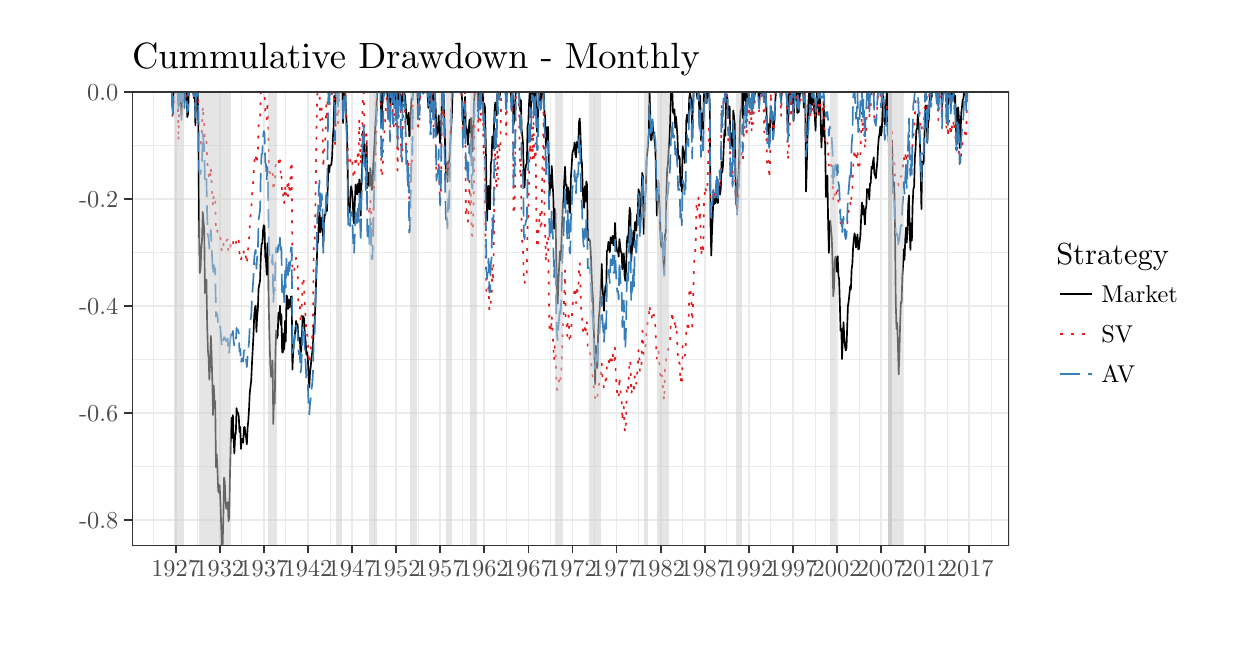
\begin{tikzpicture}[x=1pt,y=1pt]
\definecolor{fillColor}{RGB}{255,255,255}
\path[use as bounding box,fill=fillColor,fill opacity=0.00] (0,0) rectangle (426.79,216.81);
\begin{scope}
\path[clip] (  0.00,  0.00) rectangle (426.79,216.81);
\definecolor{drawColor}{RGB}{255,255,255}
\definecolor{fillColor}{RGB}{255,255,255}

\path[draw=drawColor,line width= 0.6pt,line join=round,line cap=round,fill=fillColor] (  0.00,  0.00) rectangle (426.79,216.81);
\end{scope}
\begin{scope}
\path[clip] ( 37.70, 29.59) rectangle (354.63,193.67);
\definecolor{fillColor}{RGB}{255,255,255}

\path[fill=fillColor] ( 37.70, 29.59) rectangle (354.63,193.67);
\definecolor{drawColor}{gray}{0.92}

\path[draw=drawColor,line width= 0.3pt,line join=round] ( 37.70, 58.23) --
	(354.63, 58.23);

\path[draw=drawColor,line width= 0.3pt,line join=round] ( 37.70, 96.93) --
	(354.63, 96.93);

\path[draw=drawColor,line width= 0.3pt,line join=round] ( 37.70,135.63) --
	(354.63,135.63);

\path[draw=drawColor,line width= 0.3pt,line join=round] ( 37.70,174.33) --
	(354.63,174.33);

\path[draw=drawColor,line width= 0.3pt,line join=round] ( 45.51, 29.59) --
	( 45.51,193.67);

\path[draw=drawColor,line width= 0.3pt,line join=round] ( 61.44, 29.59) --
	( 61.44,193.67);

\path[draw=drawColor,line width= 0.3pt,line join=round] ( 77.38, 29.59) --
	( 77.38,193.67);

\path[draw=drawColor,line width= 0.3pt,line join=round] ( 93.31, 29.59) --
	( 93.31,193.67);

\path[draw=drawColor,line width= 0.3pt,line join=round] (109.24, 29.59) --
	(109.24,193.67);

\path[draw=drawColor,line width= 0.3pt,line join=round] (125.17, 29.59) --
	(125.17,193.67);

\path[draw=drawColor,line width= 0.3pt,line join=round] (141.10, 29.59) --
	(141.10,193.67);

\path[draw=drawColor,line width= 0.3pt,line join=round] (157.04, 29.59) --
	(157.04,193.67);

\path[draw=drawColor,line width= 0.3pt,line join=round] (172.97, 29.59) --
	(172.97,193.67);

\path[draw=drawColor,line width= 0.3pt,line join=round] (188.90, 29.59) --
	(188.90,193.67);

\path[draw=drawColor,line width= 0.3pt,line join=round] (204.83, 29.59) --
	(204.83,193.67);

\path[draw=drawColor,line width= 0.3pt,line join=round] (220.77, 29.59) --
	(220.77,193.67);

\path[draw=drawColor,line width= 0.3pt,line join=round] (236.70, 29.59) --
	(236.70,193.67);

\path[draw=drawColor,line width= 0.3pt,line join=round] (252.63, 29.59) --
	(252.63,193.67);

\path[draw=drawColor,line width= 0.3pt,line join=round] (268.56, 29.59) --
	(268.56,193.67);

\path[draw=drawColor,line width= 0.3pt,line join=round] (284.49, 29.59) --
	(284.49,193.67);

\path[draw=drawColor,line width= 0.3pt,line join=round] (300.42, 29.59) --
	(300.42,193.67);

\path[draw=drawColor,line width= 0.3pt,line join=round] (316.35, 29.59) --
	(316.35,193.67);

\path[draw=drawColor,line width= 0.3pt,line join=round] (332.29, 29.59) --
	(332.29,193.67);

\path[draw=drawColor,line width= 0.3pt,line join=round] (348.22, 29.59) --
	(348.22,193.67);

\path[draw=drawColor,line width= 0.6pt,line join=round] ( 37.70, 38.88) --
	(354.63, 38.88);

\path[draw=drawColor,line width= 0.6pt,line join=round] ( 37.70, 77.58) --
	(354.63, 77.58);

\path[draw=drawColor,line width= 0.6pt,line join=round] ( 37.70,116.28) --
	(354.63,116.28);

\path[draw=drawColor,line width= 0.6pt,line join=round] ( 37.70,154.98) --
	(354.63,154.98);

\path[draw=drawColor,line width= 0.6pt,line join=round] ( 37.70,193.67) --
	(354.63,193.67);

\path[draw=drawColor,line width= 0.6pt,line join=round] ( 53.48, 29.59) --
	( 53.48,193.67);

\path[draw=drawColor,line width= 0.6pt,line join=round] ( 69.41, 29.59) --
	( 69.41,193.67);

\path[draw=drawColor,line width= 0.6pt,line join=round] ( 85.34, 29.59) --
	( 85.34,193.67);

\path[draw=drawColor,line width= 0.6pt,line join=round] (101.27, 29.59) --
	(101.27,193.67);

\path[draw=drawColor,line width= 0.6pt,line join=round] (117.20, 29.59) --
	(117.20,193.67);

\path[draw=drawColor,line width= 0.6pt,line join=round] (133.13, 29.59) --
	(133.13,193.67);

\path[draw=drawColor,line width= 0.6pt,line join=round] (149.07, 29.59) --
	(149.07,193.67);

\path[draw=drawColor,line width= 0.6pt,line join=round] (165.00, 29.59) --
	(165.00,193.67);

\path[draw=drawColor,line width= 0.6pt,line join=round] (180.93, 29.59) --
	(180.93,193.67);

\path[draw=drawColor,line width= 0.6pt,line join=round] (196.86, 29.59) --
	(196.86,193.67);

\path[draw=drawColor,line width= 0.6pt,line join=round] (212.80, 29.59) --
	(212.80,193.67);

\path[draw=drawColor,line width= 0.6pt,line join=round] (228.73, 29.59) --
	(228.73,193.67);

\path[draw=drawColor,line width= 0.6pt,line join=round] (244.66, 29.59) --
	(244.66,193.67);

\path[draw=drawColor,line width= 0.6pt,line join=round] (260.59, 29.59) --
	(260.59,193.67);

\path[draw=drawColor,line width= 0.6pt,line join=round] (276.53, 29.59) --
	(276.53,193.67);

\path[draw=drawColor,line width= 0.6pt,line join=round] (292.46, 29.59) --
	(292.46,193.67);

\path[draw=drawColor,line width= 0.6pt,line join=round] (308.39, 29.59) --
	(308.39,193.67);

\path[draw=drawColor,line width= 0.6pt,line join=round] (324.32, 29.59) --
	(324.32,193.67);

\path[draw=drawColor,line width= 0.6pt,line join=round] (340.26, 29.59) --
	(340.26,193.67);
\definecolor{drawColor}{RGB}{0,0,0}

\path[draw=drawColor,line width= 0.6pt,line join=round] ( 52.11,193.67) --
	( 52.38,187.60) --
	( 52.65,192.50) --
	( 52.91,193.67) --
	( 53.18,193.54) --
	( 53.44,193.67) --
	( 53.71,193.67) --
	( 53.98,193.67) --
	( 54.23,193.67) --
	( 54.50,189.12) --
	( 54.76,193.67) --
	( 55.03,193.67) --
	( 55.29,193.67) --
	( 55.56,185.27) --
	( 55.83,193.67) --
	( 56.09,193.67) --
	( 56.36,192.62) --
	( 56.63,189.42) --
	( 56.90,193.67) --
	( 57.17,193.67) --
	( 57.42,193.67) --
	( 57.69,184.51) --
	( 57.95,185.65) --
	( 58.22,193.67) --
	( 58.48,193.67) --
	( 58.75,193.67) --
	( 59.02,193.67) --
	( 59.29,193.67) --
	( 59.56,193.67) --
	( 59.82,193.47) --
	( 60.09,191.31) --
	( 60.36,193.67) --
	( 60.60,181.46) --
	( 60.87,193.67) --
	( 61.14,193.67) --
	( 61.41,193.67) --
	( 61.67,183.31) --
	( 61.94,146.70) --
	( 62.21,128.11) --
	( 62.47,129.62) --
	( 62.74,136.67) --
	( 63.00,140.01) --
	( 63.27,150.23) --
	( 63.54,146.71) --
	( 63.79,144.16) --
	( 64.06,120.87) --
	( 64.32,125.61) --
	( 64.59,125.73) --
	( 64.85,109.84) --
	( 65.12,100.26) --
	( 65.39, 97.23) --
	( 65.65, 89.61) --
	( 65.92, 95.19) --
	( 66.19,105.46) --
	( 66.46, 98.70) --
	( 66.73, 88.79) --
	( 66.97, 76.83) --
	( 67.24, 87.52) --
	( 67.50, 81.64) --
	( 67.77, 81.83) --
	( 68.04, 57.97) --
	( 68.31, 62.67) --
	( 68.58, 57.12) --
	( 68.84, 49.39) --
	( 69.11, 48.79) --
	( 69.37, 51.53) --
	( 69.64, 45.75) --
	( 69.91, 37.49) --
	( 70.16, 29.75) --
	( 70.44, 29.59) --
	( 70.70, 39.58) --
	( 70.97, 54.20) --
	( 71.23, 52.64) --
	( 71.50, 45.67) --
	( 71.77, 43.01) --
	( 72.03, 44.94) --
	( 72.30, 45.37) --
	( 72.56, 38.44) --
	( 72.83, 39.70) --
	( 73.10, 55.30) --
	( 73.35, 67.02) --
	( 73.62, 75.86) --
	( 73.88, 68.54) --
	( 74.15, 76.82) --
	( 74.41, 68.69) --
	( 74.68, 62.94) --
	( 74.95, 69.20) --
	( 75.22, 70.43) --
	( 75.49, 79.32) --
	( 75.75, 77.38) --
	( 76.02, 77.68) --
	( 76.29, 76.25) --
	( 76.53, 70.73) --
	( 76.80, 72.51) --
	( 77.07, 64.60) --
	( 77.34, 68.27) --
	( 77.60, 68.10) --
	( 77.87, 66.81) --
	( 78.14, 72.27) --
	( 78.40, 72.52) --
	( 78.67, 70.09) --
	( 78.93, 68.73) --
	( 79.20, 66.25) --
	( 79.47, 72.21) --
	( 79.72, 74.70) --
	( 79.99, 79.00) --
	( 80.25, 84.83) --
	( 80.52, 87.09) --
	( 80.78, 89.35) --
	( 81.05, 95.53) --
	( 81.32,100.56) --
	( 81.58,105.26) --
	( 81.85,112.55) --
	( 82.12,115.39) --
	( 82.39,116.33) --
	( 82.66,106.85) --
	( 82.91,112.38) --
	( 83.18,115.13) --
	( 83.44,122.68) --
	( 83.71,123.99) --
	( 83.97,125.45) --
	( 84.25,134.19) --
	( 84.52,138.58) --
	( 84.78,138.94) --
	( 85.05,143.54) --
	( 85.31,145.42) --
	( 85.58,145.01) --
	( 85.85,134.06) --
	( 86.09,133.10) --
	( 86.37,127.51) --
	( 86.63,138.85) --
	( 86.90,132.11) --
	( 87.16,114.05) --
	( 87.43,103.12) --
	( 87.70, 94.53) --
	( 87.96, 90.67) --
	( 88.23, 91.26) --
	( 88.49, 96.55) --
	( 88.76, 73.57) --
	( 89.03, 84.28) --
	( 89.28, 81.01) --
	( 89.55,100.23) --
	( 89.81,107.44) --
	( 90.08,104.53) --
	( 90.34,105.47) --
	( 90.61,113.78) --
	( 90.88,111.69) --
	( 91.15,116.35) --
	( 91.42,109.40) --
	( 91.68,113.25) --
	( 91.95, 99.61) --
	( 92.22, 99.41) --
	( 92.46,106.27) --
	( 92.73,100.58) --
	( 93.00,110.83) --
	( 93.27,103.38) --
	( 93.53,120.08) --
	( 93.80,119.59) --
	( 94.07,115.14) --
	( 94.33,118.55) --
	( 94.60,115.69) --
	( 94.86,117.39) --
	( 95.13,119.58) --
	( 95.40,119.68) --
	( 95.66, 93.25) --
	( 95.93, 99.48) --
	( 96.19,102.67) --
	( 96.46,105.16) --
	( 96.72,107.57) --
	( 96.99,110.82) --
	( 97.26,108.97) --
	( 97.52,109.68) --
	( 97.79,105.17) --
	( 98.06,103.72) --
	( 98.33,104.72) --
	( 98.60, 99.08) --
	( 98.84,100.37) --
	( 99.11,106.24) --
	( 99.37,112.56) --
	( 99.64,112.43) --
	( 99.90,111.54) --
	(100.17,105.63) --
	(100.45,103.49) --
	(100.71, 98.66) --
	(100.98, 99.55) --
	(101.24, 97.19) --
	(101.51, 90.85) --
	(101.78, 86.89) --
	(102.02, 92.10) --
	(102.29, 94.46) --
	(102.56, 97.76) --
	(102.83, 99.53) --
	(103.09,102.19) --
	(103.36,109.21) --
	(103.63,109.30) --
	(103.89,114.87) --
	(104.16,123.25) --
	(104.42,130.65) --
	(104.69,138.67) --
	(104.96,139.64) --
	(105.21,147.57) --
	(105.48,150.08) --
	(105.74,142.88) --
	(106.01,144.75) --
	(106.27,148.19) --
	(106.54,146.43) --
	(106.81,137.63) --
	(107.08,146.42) --
	(107.35,149.01) --
	(107.61,149.48) --
	(107.88,153.13) --
	(108.15,150.56) --
	(108.40,158.19) --
	(108.67,167.12) --
	(108.93,164.53) --
	(109.20,167.05) --
	(109.47,167.07) --
	(109.74,167.37) --
	(110.01,170.13) --
	(110.27,177.05) --
	(110.54,180.58) --
	(110.80,192.17) --
	(111.07,184.59) --
	(111.34,193.67) --
	(111.59,193.67) --
	(111.86,193.67) --
	(112.12,189.35) --
	(112.39,193.67) --
	(112.65,193.67) --
	(112.92,193.67) --
	(113.19,193.67) --
	(113.45,193.67) --
	(113.72,193.67) --
	(113.98,182.35) --
	(114.26,192.84) --
	(114.53,193.67) --
	(114.77,193.67) --
	(115.04,186.14) --
	(115.30,181.19) --
	(115.57,169.47) --
	(115.83,152.15) --
	(116.10,149.96) --
	(116.38,150.02) --
	(116.64,157.48) --
	(116.91,159.49) --
	(117.17,157.68) --
	(117.44,154.99) --
	(117.71,147.56) --
	(117.95,146.10) --
	(118.22,153.82) --
	(118.49,160.12) --
	(118.76,157.30) --
	(119.02,156.52) --
	(119.29,160.35) --
	(119.56,157.26) --
	(119.82,161.98) --
	(120.09,155.76) --
	(120.35,148.88) --
	(120.62,161.06) --
	(120.89,167.07) --
	(121.15,179.32) --
	(121.42,179.12) --
	(121.68,169.99) --
	(121.95,170.47) --
	(122.21,165.26) --
	(122.48,175.06) --
	(122.75,158.90) --
	(123.01,164.00) --
	(123.28,164.44) --
	(123.55,159.64) --
	(123.82,166.09) --
	(124.09,162.97) --
	(124.33,158.17) --
	(124.60,158.37) --
	(124.86,167.12) --
	(125.13,171.45) --
	(125.40,176.78) --
	(125.67,182.23) --
	(125.94,185.44) --
	(126.20,193.67) --
	(126.47,193.67) --
	(126.73,193.67) --
	(127.00,193.67) --
	(127.27,193.67) --
	(127.52,193.67) --
	(127.79,182.28) --
	(128.05,185.04) --
	(128.32,193.67) --
	(128.58,193.67) --
	(128.85,193.25) --
	(129.12,193.67) --
	(129.38,193.67) --
	(129.65,193.67) --
	(129.91,193.67) --
	(130.19,189.34) --
	(130.46,193.67) --
	(130.70,189.12) --
	(130.97,184.06) --
	(131.23,193.67) --
	(131.50,193.67) --
	(131.76,193.67) --
	(132.03,189.05) --
	(132.31,189.99) --
	(132.57,193.67) --
	(132.84,193.67) --
	(133.10,188.58) --
	(133.37,193.67) --
	(133.64,183.94) --
	(133.89,189.77) --
	(134.16,193.67) --
	(134.43,193.67) --
	(134.70,192.08) --
	(134.96,188.13) --
	(135.23,186.85) --
	(135.50,193.67) --
	(135.76,193.67) --
	(136.03,193.16) --
	(136.29,192.50) --
	(136.56,189.73) --
	(136.83,184.22) --
	(137.08,185.16) --
	(137.35,181.84) --
	(137.61,186.09) --
	(137.88,177.58) --
	(138.14,177.84) --
	(138.41,185.97) --
	(138.68,190.96) --
	(138.94,190.84) --
	(139.21,193.67) --
	(139.48,193.67) --
	(139.75,193.67) --
	(140.02,193.67) --
	(140.26,193.67) --
	(140.53,193.67) --
	(140.79,193.67) --
	(141.06,189.16) --
	(141.33,193.67) --
	(141.60,190.44) --
	(141.87,193.67) --
	(142.13,193.67) --
	(142.40,193.67) --
	(142.66,193.67) --
	(142.93,193.33) --
	(143.20,193.67) --
	(143.45,193.67) --
	(143.72,193.67) --
	(143.98,193.67) --
	(144.25,193.67) --
	(144.51,193.09) --
	(144.78,187.83) --
	(145.05,193.67) --
	(145.31,193.67) --
	(145.58,187.91) --
	(145.84,193.67) --
	(146.12,193.67) --
	(146.39,193.67) --
	(146.64,183.86) --
	(146.91,190.34) --
	(147.17,193.67) --
	(147.44,187.53) --
	(147.70,177.85) --
	(147.97,178.84) --
	(148.24,179.35) --
	(148.51,185.15) --
	(148.78,178.85) --
	(149.04,175.09) --
	(149.31,178.83) --
	(149.58,186.45) --
	(149.82,192.84) --
	(150.09,191.39) --
	(150.35,192.60) --
	(150.63,182.53) --
	(150.89,171.51) --
	(151.16,164.04) --
	(151.43,167.80) --
	(151.69,161.07) --
	(151.96,168.57) --
	(152.22,165.78) --
	(152.49,170.88) --
	(152.76,175.93) --
	(153.01,180.09) --
	(153.28,185.25) --
	(153.54,193.33) --
	(153.81,193.67) --
	(154.07,193.67) --
	(154.34,193.67) --
	(154.61,193.67) --
	(154.87,193.67) --
	(155.14,193.67) --
	(155.41,193.67) --
	(155.68,193.67) --
	(155.95,193.67) --
	(156.19,193.67) --
	(156.46,193.42) --
	(156.72,193.67) --
	(156.99,190.79) --
	(157.26,181.76) --
	(157.53,184.27) --
	(157.80,187.11) --
	(158.06,191.78) --
	(158.33,178.62) --
	(158.59,180.58) --
	(158.86,177.68) --
	(159.13,174.47) --
	(159.38,179.78) --
	(159.65,183.53) --
	(159.92,178.89) --
	(160.19,184.20) --
	(160.45,173.18) --
	(160.72,172.07) --
	(160.99,180.14) --
	(161.25,188.46) --
	(161.52,193.67) --
	(161.78,193.67) --
	(162.05,193.67) --
	(162.32,193.67) --
	(162.57,193.67) --
	(162.84,187.84) --
	(163.10,193.12) --
	(163.37,193.67) --
	(163.63,189.47) --
	(163.90,193.67) --
	(164.17,193.67) --
	(164.44,193.45) --
	(164.71,186.18) --
	(164.97,189.45) --
	(165.24,188.11) --
	(165.51,175.84) --
	(165.75,160.65) --
	(166.02,147.07) --
	(166.28,156.31) --
	(166.56,159.65) --
	(166.82,151.24) --
	(167.09,151.22) --
	(167.36,167.51) --
	(167.62,169.07) --
	(167.89,177.47) --
	(168.15,173.19) --
	(168.42,178.44) --
	(168.69,186.46) --
	(168.94,189.76) --
	(169.21,185.88) --
	(169.47,185.12) --
	(169.74,193.67) --
	(170.00,190.86) --
	(170.27,193.67) --
	(170.54,192.08) --
	(170.80,193.67) --
	(171.07,193.67) --
	(171.34,193.67) --
	(171.61,193.67) --
	(171.88,193.67) --
	(172.13,193.67) --
	(172.40,193.67) --
	(172.66,193.67) --
	(172.93,190.92) --
	(173.19,193.67) --
	(173.46,193.67) --
	(173.74,193.67) --
	(174.00,193.67) --
	(174.27,193.67) --
	(174.53,193.67) --
	(174.80,191.26) --
	(175.07,193.67) --
	(175.31,192.14) --
	(175.58,181.62) --
	(175.85,184.09) --
	(176.12,189.11) --
	(176.38,193.67) --
	(176.65,193.67) --
	(176.92,193.67) --
	(177.18,193.67) --
	(177.45,193.67) --
	(177.71,191.38) --
	(177.98,186.67) --
	(178.25,190.63) --
	(178.50,179.94) --
	(178.77,177.49) --
	(179.03,174.49) --
	(179.30,160.74) --
	(179.56,159.06) --
	(179.83,165.11) --
	(180.10,167.33) --
	(180.37,167.61) --
	(180.64,181.21) --
	(180.90,182.46) --
	(181.17,189.56) --
	(181.44,193.67) --
	(181.68,185.35) --
	(181.95,189.72) --
	(182.21,193.67) --
	(182.49,191.94) --
	(182.75,193.67) --
	(183.02,187.79) --
	(183.29,188.66) --
	(183.55,193.67) --
	(183.82,185.98) --
	(184.08,179.14) --
	(184.35,179.34) --
	(184.62,193.67) --
	(184.88,193.67) --
	(185.15,193.67) --
	(185.41,188.57) --
	(185.68,191.14) --
	(185.94,193.67) --
	(186.21,193.67) --
	(186.48,193.67) --
	(186.74,186.30) --
	(187.01,184.28) --
	(187.27,173.66) --
	(187.55,178.01) --
	(187.82,180.83) --
	(188.06,180.91) --
	(188.33,167.84) --
	(188.59,156.16) --
	(188.86,163.36) --
	(189.12,158.84) --
	(189.39,166.83) --
	(189.66,160.48) --
	(189.93,156.38) --
	(190.20,144.19) --
	(190.46,151.39) --
	(190.73,149.78) --
	(191.00,133.20) --
	(191.24,123.93) --
	(191.51,117.03) --
	(191.78,125.03) --
	(192.05,130.53) --
	(192.31,136.01) --
	(192.58,132.84) --
	(192.85,138.78) --
	(193.11,146.53) --
	(193.38,153.43) --
	(193.64,155.37) --
	(193.91,161.71) --
	(194.18,166.55) --
	(194.43,160.01) --
	(194.70,160.06) --
	(194.96,153.18) --
	(195.23,159.09) --
	(195.49,157.66) --
	(195.76,150.55) --
	(196.03,149.81) --
	(196.30,162.86) --
	(196.57,166.86) --
	(196.83,171.45) --
	(197.10,172.45) --
	(197.37,172.96) --
	(197.62,175.32) --
	(197.89,171.16) --
	(198.15,169.93) --
	(198.42,175.52) --
	(198.69,173.64) --
	(198.96,174.64) --
	(199.23,182.70) --
	(199.49,184.02) --
	(199.76,178.31) --
	(200.02,169.78) --
	(200.29,167.71) --
	(200.56,158.39) --
	(200.81,153.81) --
	(201.08,151.69) --
	(201.34,159.51) --
	(201.61,154.00) --
	(201.87,161.26) --
	(202.14,160.08) --
	(202.41,139.83) --
	(202.67,140.51) --
	(202.94,140.35) --
	(203.20,139.78) --
	(203.47,135.67) --
	(203.75,128.69) --
	(203.99,122.61) --
	(204.26,118.91) --
	(204.52,109.68) --
	(204.79, 99.47) --
	(205.05, 87.96) --
	(205.32,101.89) --
	(205.59, 96.93) --
	(205.86, 93.84) --
	(206.13,106.53) --
	(206.39,111.96) --
	(206.66,114.67) --
	(206.93,119.48) --
	(207.17,125.54) --
	(207.44,131.42) --
	(207.71,122.95) --
	(207.98,119.57) --
	(208.24,114.48) --
	(208.51,120.29) --
	(208.78,123.39) --
	(209.04,121.36) --
	(209.31,136.07) --
	(209.57,136.41) --
	(209.84,139.40) --
	(210.11,137.49) --
	(210.37,135.66) --
	(210.64,141.10) --
	(210.90,139.71) --
	(211.17,138.92) --
	(211.43,141.65) --
	(211.70,138.19) --
	(211.97,138.32) --
	(212.23,146.23) --
	(212.50,140.36) --
	(212.77,137.60) --
	(213.04,135.84) --
	(213.31,136.04) --
	(213.55,134.07) --
	(213.82,140.41) --
	(214.08,138.10) --
	(214.35,135.72) --
	(214.62,135.37) --
	(214.89,129.49) --
	(215.16,134.78) --
	(215.42,135.23) --
	(215.69,127.14) --
	(215.95,125.35) --
	(216.22,128.97) --
	(216.49,139.01) --
	(216.74,141.48) --
	(217.01,139.21) --
	(217.27,146.36) --
	(217.54,151.73) --
	(217.80,149.85) --
	(218.07,132.49) --
	(218.34,136.12) --
	(218.60,137.59) --
	(218.87,143.39) --
	(219.13,138.48) --
	(219.40,146.43) --
	(219.68,146.60) --
	(219.92,143.46) --
	(220.19,148.98) --
	(220.45,149.98) --
	(220.72,158.40) --
	(220.98,157.41) --
	(221.25,144.87) --
	(221.52,152.81) --
	(221.79,155.76) --
	(222.06,164.34) --
	(222.32,162.96) --
	(222.59,142.26) --
	(222.86,148.37) --
	(223.11,155.39) --
	(223.38,159.24) --
	(223.64,168.92) --
	(223.92,171.85) --
	(224.18,175.98) --
	(224.45,178.37) --
	(224.72,193.67) --
	(224.98,185.26) --
	(225.25,176.15) --
	(225.51,176.57) --
	(225.78,182.82) --
	(226.05,178.85) --
	(226.30,179.10) --
	(226.57,175.38) --
	(226.83,172.85) --
	(227.10,160.97) --
	(227.36,148.87) --
	(227.63,155.82) --
	(227.90,160.96) --
	(228.16,154.58) --
	(228.43,148.94) --
	(228.70,140.12) --
	(228.97,137.60) --
	(229.24,142.24) --
	(229.48,136.90) --
	(229.75,132.14) --
	(230.01,128.07) --
	(230.28,141.93) --
	(230.55,142.81) --
	(230.82,158.53) --
	(231.09,165.90) --
	(231.35,167.32) --
	(231.62,173.23) --
	(231.88,177.27) --
	(232.15,182.16) --
	(232.42,193.67) --
	(232.67,193.67) --
	(232.94,193.67) --
	(233.20,186.28) --
	(233.47,185.68) --
	(233.73,187.28) --
	(234.00,180.65) --
	(234.27,184.59) --
	(234.53,181.28) --
	(234.80,177.68) --
	(235.06,169.51) --
	(235.33,170.48) --
	(235.61,169.71) --
	(235.86,159.67) --
	(236.13,162.09) --
	(236.39,157.52) --
	(236.66,173.95) --
	(236.92,172.61) --
	(237.19,171.18) --
	(237.46,167.91) --
	(237.73,170.17) --
	(238.00,183.41) --
	(238.26,185.32) --
	(238.53,183.80) --
	(238.80,182.34) --
	(239.04,191.32) --
	(239.31,193.20) --
	(239.57,191.88) --
	(239.84,189.92) --
	(240.11,181.24) --
	(240.38,188.25) --
	(240.65,193.67) --
	(240.91,193.67) --
	(241.18,193.67) --
	(241.44,193.67) --
	(241.71,193.67) --
	(241.98,191.13) --
	(242.23,193.67) --
	(242.50,193.67) --
	(242.76,181.24) --
	(243.03,192.22) --
	(243.29,176.13) --
	(243.56,183.96) --
	(243.83,185.90) --
	(244.09,180.17) --
	(244.36,193.67) --
	(244.63,193.67) --
	(244.90,193.67) --
	(245.17,189.57) --
	(245.41,189.65) --
	(245.68,193.67) --
	(245.94,193.67) --
	(246.21,193.67) --
	(246.48,188.79) --
	(246.75,145.60) --
	(247.02,134.49) --
	(247.28,143.07) --
	(247.55,148.97) --
	(247.81,156.05) --
	(248.08,153.02) --
	(248.35,153.99) --
	(248.60,153.39) --
	(248.87,160.53) --
	(249.14,158.56) --
	(249.41,153.37) --
	(249.67,158.26) --
	(249.94,160.11) --
	(250.21,156.52) --
	(250.47,158.84) --
	(250.74,168.37) --
	(251.00,164.57) --
	(251.27,167.18) --
	(251.54,174.17) --
	(251.79,179.81) --
	(252.06,177.75) --
	(252.32,189.94) --
	(252.59,192.78) --
	(252.85,191.15) --
	(253.12,184.20) --
	(253.39,186.27) --
	(253.65,188.39) --
	(253.93,174.00) --
	(254.19,175.52) --
	(254.46,178.73) --
	(254.73,172.70) --
	(254.97,186.85) --
	(255.24,184.79) --
	(255.50,181.82) --
	(255.77,164.09) --
	(256.04,154.22) --
	(256.31,151.30) --
	(256.58,160.27) --
	(256.84,163.88) --
	(257.11,170.94) --
	(257.37,182.80) --
	(257.64,187.11) --
	(257.91,186.83) --
	(258.16,193.58) --
	(258.43,184.09) --
	(258.69,191.80) --
	(258.96,193.67) --
	(259.22,190.62) --
	(259.49,193.12) --
	(259.76,185.08) --
	(260.02,193.67) --
	(260.29,192.70) --
	(260.56,193.67) --
	(260.83,188.45) --
	(261.10,190.44) --
	(261.35,191.02) --
	(261.62,186.74) --
	(261.88,193.65) --
	(262.15,189.01) --
	(262.41,190.77) --
	(262.68,192.37) --
	(262.95,193.67) --
	(263.22,193.67) --
	(263.49,193.67) --
	(263.75,193.67) --
	(264.02,193.67) --
	(264.29,188.35) --
	(264.53,193.43) --
	(264.80,193.67) --
	(265.07,193.10) --
	(265.34,193.67) --
	(265.60,193.34) --
	(265.87,193.67) --
	(266.14,189.78) --
	(266.40,193.05) --
	(266.67,193.67) --
	(266.93,188.55) --
	(267.20,179.48) --
	(267.47,180.80) --
	(267.72,182.00) --
	(267.99,176.45) --
	(268.25,181.29) --
	(268.52,188.42) --
	(268.78,184.45) --
	(269.05,186.43) --
	(269.32,178.84) --
	(269.58,180.41) --
	(269.86,183.41) --
	(270.12,189.83) --
	(270.39,193.67) --
	(270.66,193.67) --
	(270.90,193.67) --
	(271.17,193.67) --
	(271.43,193.67) --
	(271.70,193.67) --
	(271.97,193.67) --
	(272.24,190.59) --
	(272.51,193.67) --
	(272.77,193.67) --
	(273.04,193.67) --
	(273.30,193.67) --
	(273.57,193.67) --
	(273.84,193.67) --
	(274.10,193.67) --
	(274.37,191.19) --
	(274.63,180.16) --
	(274.90,185.25) --
	(275.16,193.67) --
	(275.43,193.67) --
	(275.70,193.67) --
	(275.96,190.67) --
	(276.23,193.67) --
	(276.49,192.57) --
	(276.76,183.12) --
	(277.04,190.13) --
	(277.28,193.67) --
	(277.55,193.67) --
	(277.81,193.67) --
	(278.08,185.97) --
	(278.34,193.67) --
	(278.61,186.25) --
	(278.88,191.07) --
	(279.15,193.65) --
	(279.42,193.67) --
	(279.68,193.67) --
	(279.95,193.67) --
	(280.22,193.67) --
	(280.46,187.96) --
	(280.73,193.13) --
	(281.00,187.87) --
	(281.27,157.60) --
	(281.53,166.98) --
	(281.80,178.62) --
	(282.07,188.82) --
	(282.33,193.67) --
	(282.60,193.67) --
	(282.86,185.60) --
	(283.13,191.96) --
	(283.40,193.67) --
	(283.65,188.86) --
	(283.92,193.67) --
	(284.18,187.10) --
	(284.45,184.49) --
	(284.71,179.60) --
	(284.98,190.01) --
	(285.25,193.67) --
	(285.51,193.67) --
	(285.79,185.34) --
	(286.05,190.39) --
	(286.32,193.67) --
	(286.59,181.38) --
	(286.84,173.52) --
	(287.11,181.63) --
	(287.37,177.53) --
	(287.64,190.07) --
	(287.91,179.50) --
	(288.18,174.24) --
	(288.45,155.63) --
	(288.71,157.92) --
	(288.98,163.33) --
	(289.24,146.43) --
	(289.51,135.41) --
	(289.78,146.19) --
	(290.02,147.10) --
	(290.30,143.96) --
	(290.56,140.88) --
	(290.83,132.21) --
	(291.09,119.77) --
	(291.36,122.72) --
	(291.63,132.00) --
	(291.89,134.06) --
	(292.16,131.70) --
	(292.42,128.65) --
	(292.69,134.21) --
	(292.96,127.39) --
	(293.21,125.89) --
	(293.48,116.88) --
	(293.74,107.26) --
	(294.01,107.98) --
	(294.27, 97.06) --
	(294.54,104.17) --
	(294.81,110.39) --
	(295.08,104.37) --
	(295.35,101.81) --
	(295.61,100.14) --
	(295.88,101.07) --
	(296.15,109.32) --
	(296.39,116.13) --
	(296.66,117.91) --
	(296.93,120.52) --
	(297.20,123.40) --
	(297.46,122.19) --
	(297.73,129.46) --
	(298.00,131.50) --
	(298.26,137.38) --
	(298.53,140.44) --
	(298.79,142.50) --
	(299.06,140.88) --
	(299.33,137.39) --
	(299.59,139.19) --
	(299.86,142.08) --
	(300.12,136.66) --
	(300.39,136.92) --
	(300.65,139.59) --
	(300.92,141.91) --
	(301.19,148.58) --
	(301.45,153.63) --
	(301.72,149.33) --
	(301.99,152.47) --
	(302.26,149.65) --
	(302.53,145.66) --
	(302.77,150.86) --
	(303.04,152.28) --
	(303.30,158.49) --
	(303.57,157.19) --
	(303.83,158.47) --
	(304.11,154.70) --
	(304.38,160.47) --
	(304.64,160.59) --
	(304.91,166.50) --
	(305.17,165.70) --
	(305.44,168.26) --
	(305.71,169.87) --
	(305.95,163.99) --
	(306.23,163.34) --
	(306.49,162.34) --
	(306.76,165.74) --
	(307.02,168.28) --
	(307.29,173.79) --
	(307.56,177.18) --
	(307.82,178.37) --
	(308.09,181.07) --
	(308.35,177.83) --
	(308.62,179.34) --
	(308.89,185.77) --
	(309.14,192.17) --
	(309.41,188.51) --
	(309.67,181.78) --
	(309.94,183.16) --
	(310.20,189.88) --
	(310.47,193.67) --
	(310.74,183.54) --
	(311.01,182.15) --
	(311.28,170.26) --
	(311.54,166.13) --
	(311.81,164.06) --
	(312.08,172.21) --
	(312.33,176.01) --
	(312.60,161.93) --
	(312.86,159.49) --
	(313.13,160.90) --
	(313.40,144.93) --
	(313.67,118.05) --
	(313.94,107.92) --
	(314.20,110.21) --
	(314.47,101.68) --
	(314.73, 91.50) --
	(315.00, 99.42) --
	(315.27,110.26) --
	(315.52,117.70) --
	(315.79,117.33) --
	(316.05,126.90) --
	(316.32,130.87) --
	(316.58,136.77) --
	(316.85,132.93) --
	(317.12,140.50) --
	(317.38,144.48) --
	(317.65,139.13) --
	(317.92,143.95) --
	(318.19,153.09) --
	(318.46,156.16) --
	(318.70,143.80) --
	(318.97,136.50) --
	(319.23,146.07) --
	(319.50,139.81) --
	(319.76,152.57) --
	(320.04,158.43) --
	(320.31,159.22) --
	(320.57,169.88) --
	(320.84,173.12) --
	(321.10,179.70) --
	(321.37,180.29) --
	(321.64,185.43) --
	(321.88,182.65) --
	(322.16,179.29) --
	(322.42,175.27) --
	(322.69,165.21) --
	(322.95,151.20) --
	(323.22,168.40) --
	(323.49,167.35) --
	(323.75,167.97) --
	(324.02,177.04) --
	(324.28,184.32) --
	(324.55,188.74) --
	(324.82,187.46) --
	(325.08,175.19) --
	(325.35,181.87) --
	(325.61,183.71) --
	(325.88,188.53) --
	(326.14,193.53) --
	(326.41,190.79) --
	(326.68,191.95) --
	(326.94,193.67) --
	(327.22,193.67) --
	(327.48,193.67) --
	(327.75,193.67) --
	(328.02,193.67) --
	(328.26,193.67) --
	(328.53,190.76) --
	(328.79,193.67) --
	(329.06,188.70) --
	(329.33,193.67) --
	(329.60,193.67) --
	(329.87,193.67) --
	(330.13,193.67) --
	(330.40,187.88) --
	(330.66,193.67) --
	(330.93,193.67) --
	(331.20,193.67) --
	(331.45,193.67) --
	(331.72,193.67) --
	(331.98,189.70) --
	(332.25,193.67) --
	(332.51,188.81) --
	(332.78,192.81) --
	(333.05,193.67) --
	(333.31,192.98) --
	(333.58,187.74) --
	(333.85,193.67) --
	(334.12,191.65) --
	(334.39,193.33) --
	(334.63,193.67) --
	(334.90,189.95) --
	(335.16,192.24) --
	(335.43,180.72) --
	(335.69,174.63) --
	(335.97,187.53) --
	(336.24,187.99) --
	(336.50,183.81) --
	(336.77,173.34) --
	(337.03,173.44) --
	(337.30,185.63) --
	(337.57,187.78) --
	(337.82,190.42) --
	(338.09,191.00) --
	(338.36,193.67) --
	(338.63,193.67) --
	(338.89,193.67) --
	(339.16,189.46) --
	(339.43,193.67) --
	(339.69,193.67) --
	(339.96,193.67) --
	(340.22,193.67);
\definecolor{drawColor}{RGB}{228,26,28}

\path[draw=drawColor,line width= 0.6pt,dash pattern=on 1pt off 3pt ,line join=round] ( 52.11,193.67) --
	( 52.38,183.63) --
	( 52.65,186.32) --
	( 52.91,193.67) --
	( 53.18,193.37) --
	( 53.44,193.67) --
	( 53.71,193.67) --
	( 53.98,193.67) --
	( 54.23,193.67) --
	( 54.50,175.92) --
	( 54.76,191.84) --
	( 55.03,193.67) --
	( 55.29,193.67) --
	( 55.56,185.02) --
	( 55.83,193.67) --
	( 56.09,193.67) --
	( 56.36,191.71) --
	( 56.63,187.99) --
	( 56.90,193.67) --
	( 57.17,193.67) --
	( 57.42,193.67) --
	( 57.69,188.53) --
	( 57.95,188.80) --
	( 58.22,193.67) --
	( 58.48,193.67) --
	( 58.75,193.67) --
	( 59.02,193.67) --
	( 59.29,193.67) --
	( 59.56,193.67) --
	( 59.82,193.53) --
	( 60.09,192.78) --
	( 60.36,193.38) --
	( 60.60,187.39) --
	( 60.87,191.91) --
	( 61.14,193.67) --
	( 61.41,193.67) --
	( 61.67,190.08) --
	( 61.94,175.29) --
	( 62.21,174.90) --
	( 62.47,174.95) --
	( 62.74,175.95) --
	( 63.00,180.02) --
	( 63.27,188.53) --
	( 63.54,184.04) --
	( 63.79,181.97) --
	( 64.06,175.01) --
	( 64.32,175.57) --
	( 64.59,175.61) --
	( 64.85,169.53) --
	( 65.12,164.18) --
	( 65.39,163.71) --
	( 65.65,161.62) --
	( 65.92,162.95) --
	( 66.19,166.49) --
	( 66.46,161.27) --
	( 66.73,156.20) --
	( 66.97,152.34) --
	( 67.24,156.38) --
	( 67.50,155.78) --
	( 67.77,155.84) --
	( 68.04,143.05) --
	( 68.31,143.76) --
	( 68.58,143.39) --
	( 68.84,141.26) --
	( 69.11,141.17) --
	( 69.37,141.68) --
	( 69.64,140.92) --
	( 69.91,138.15) --
	( 70.16,135.71) --
	( 70.44,135.66) --
	( 70.70,137.31) --
	( 70.97,140.79) --
	( 71.23,140.64) --
	( 71.50,140.09) --
	( 71.77,139.81) --
	( 72.03,140.12) --
	( 72.30,140.30) --
	( 72.56,135.41) --
	( 72.83,135.82) --
	( 73.10,137.11) --
	( 73.35,138.34) --
	( 73.62,139.99) --
	( 73.88,139.26) --
	( 74.15,139.73) --
	( 74.41,138.27) --
	( 74.68,137.29) --
	( 74.95,137.85) --
	( 75.22,138.16) --
	( 75.49,141.17) --
	( 75.75,140.56) --
	( 76.02,140.66) --
	( 76.29,140.19) --
	( 76.53,135.18) --
	( 76.80,135.70) --
	( 77.07,133.06) --
	( 77.34,133.84) --
	( 77.60,133.79) --
	( 77.87,133.15) --
	( 78.14,136.41) --
	( 78.40,136.78) --
	( 78.67,134.78) --
	( 78.93,133.46) --
	( 79.20,131.46) --
	( 79.47,135.32) --
	( 79.72,137.43) --
	( 79.99,140.48) --
	( 80.25,145.14) --
	( 80.52,148.81) --
	( 80.78,150.35) --
	( 81.05,156.02) --
	( 81.32,159.20) --
	( 81.58,162.17) --
	( 81.85,167.37) --
	( 82.12,170.40) --
	( 82.39,171.22) --
	( 82.66,167.54) --
	( 82.91,169.41) --
	( 83.18,171.10) --
	( 83.44,181.33) --
	( 83.71,183.27) --
	( 83.97,184.43) --
	( 84.25,193.67) --
	( 84.52,193.67) --
	( 84.78,193.67) --
	( 85.05,193.67) --
	( 85.31,193.67) --
	( 85.58,193.13) --
	( 85.85,186.73) --
	( 86.09,186.46) --
	( 86.37,183.60) --
	( 86.63,190.17) --
	( 86.90,184.92) --
	( 87.16,165.84) --
	( 87.43,164.66) --
	( 87.70,164.17) --
	( 87.96,163.76) --
	( 88.23,163.96) --
	( 88.49,165.23) --
	( 88.76,157.82) --
	( 89.03,160.00) --
	( 89.28,159.55) --
	( 89.55,166.83) --
	( 89.81,168.35) --
	( 90.08,167.46) --
	( 90.34,167.80) --
	( 90.61,168.68) --
	( 90.88,167.58) --
	( 91.15,169.67) --
	( 91.42,164.06) --
	( 91.68,165.08) --
	( 91.95,155.71) --
	( 92.22,155.66) --
	( 92.46,157.06) --
	( 92.73,153.34) --
	( 93.00,159.82) --
	( 93.27,155.70) --
	( 93.53,160.07) --
	( 93.80,160.02) --
	( 94.07,155.92) --
	( 94.33,161.43) --
	( 94.60,156.59) --
	( 94.86,158.58) --
	( 95.13,168.22) --
	( 95.40,168.47) --
	( 95.66,126.14) --
	( 95.93,126.63) --
	( 96.19,127.15) --
	( 96.46,130.90) --
	( 96.72,132.07) --
	( 96.99,133.68) --
	( 97.26,131.44) --
	( 97.52,131.63) --
	( 97.79,118.20) --
	( 98.06,116.77) --
	( 98.33,117.29) --
	( 98.60,110.06) --
	( 98.84,111.13) --
	( 99.11,117.90) --
	( 99.37,126.75) --
	( 99.64,126.58) --
	( 99.90,123.31) --
	(100.17,114.82) --
	(100.45,112.48) --
	(100.71,105.73) --
	(100.98,105.88) --
	(101.24,104.43) --
	(101.51, 97.38) --
	(101.78, 95.39) --
	(102.02, 98.07) --
	(102.29,100.55) --
	(102.56,103.77) --
	(102.83,105.13) --
	(103.09,112.13) --
	(103.36,137.25) --
	(103.63,137.36) --
	(103.89,147.35) --
	(104.16,165.06) --
	(104.42,183.05) --
	(104.69,193.67) --
	(104.96,193.67) --
	(105.21,193.67) --
	(105.48,193.67) --
	(105.74,183.36) --
	(106.01,184.49) --
	(106.27,187.60) --
	(106.54,183.10) --
	(106.81,166.22) --
	(107.08,171.77) --
	(107.35,175.76) --
	(107.61,176.85) --
	(107.88,189.04) --
	(108.15,183.55) --
	(108.40,193.67) --
	(108.67,193.67) --
	(108.93,187.73) --
	(109.20,191.03) --
	(109.47,191.10) --
	(109.74,191.44) --
	(110.01,193.67) --
	(110.27,193.67) --
	(110.54,193.67) --
	(110.80,193.67) --
	(111.07,174.31) --
	(111.34,182.04) --
	(111.59,186.39) --
	(111.86,187.52) --
	(112.12,182.05) --
	(112.39,189.08) --
	(112.65,193.67) --
	(112.92,193.67) --
	(113.19,193.67) --
	(113.45,193.67) --
	(113.72,193.67) --
	(113.98,188.31) --
	(114.26,190.17) --
	(114.53,193.67) --
	(114.77,193.67) --
	(115.04,186.55) --
	(115.30,183.09) --
	(115.57,176.56) --
	(115.83,167.20) --
	(116.10,167.05) --
	(116.38,167.06) --
	(116.64,169.35) --
	(116.91,170.26) --
	(117.17,169.18) --
	(117.44,166.66) --
	(117.71,162.95) --
	(117.95,162.17) --
	(118.22,166.02) --
	(118.49,170.51) --
	(118.76,168.66) --
	(119.02,167.61) --
	(119.29,171.05) --
	(119.56,167.20) --
	(119.82,183.64) --
	(120.09,175.30) --
	(120.35,167.28) --
	(120.62,175.47) --
	(120.89,179.56) --
	(121.15,193.67) --
	(121.42,193.44) --
	(121.68,180.90) --
	(121.95,181.12) --
	(122.21,174.02) --
	(122.48,178.83) --
	(122.75,151.29) --
	(123.01,152.18) --
	(123.28,152.72) --
	(123.55,148.85) --
	(123.82,154.57) --
	(124.09,151.35) --
	(124.33,140.63) --
	(124.60,140.87) --
	(124.86,146.24) --
	(125.13,159.10) --
	(125.40,165.44) --
	(125.67,168.98) --
	(125.94,174.45) --
	(126.20,190.63) --
	(126.47,193.67) --
	(126.73,193.67) --
	(127.00,193.67) --
	(127.27,193.67) --
	(127.52,193.67) --
	(127.79,162.76) --
	(128.05,163.22) --
	(128.32,165.79) --
	(128.58,178.96) --
	(128.85,178.53) --
	(129.12,182.32) --
	(129.38,186.49) --
	(129.65,190.93) --
	(129.91,192.77) --
	(130.19,184.30) --
	(130.46,191.59) --
	(130.70,185.75) --
	(130.97,180.97) --
	(131.23,193.67) --
	(131.50,193.67) --
	(131.76,193.67) --
	(132.03,180.16) --
	(132.31,180.75) --
	(132.57,188.16) --
	(132.84,193.67) --
	(133.10,180.86) --
	(133.37,190.58) --
	(133.64,165.19) --
	(133.89,173.72) --
	(134.16,189.53) --
	(134.43,193.67) --
	(134.70,186.63) --
	(134.96,170.65) --
	(135.23,167.57) --
	(135.50,179.20) --
	(135.76,193.67) --
	(136.03,189.63) --
	(136.29,187.58) --
	(136.56,179.21) --
	(136.83,171.35) --
	(137.08,172.22) --
	(137.35,165.27) --
	(137.61,168.72) --
	(137.88,152.38) --
	(138.14,152.78) --
	(138.41,158.68) --
	(138.68,168.89) --
	(138.94,168.51) --
	(139.21,192.49) --
	(139.48,193.67) --
	(139.75,193.67) --
	(140.02,193.67) --
	(140.26,193.67) --
	(140.53,193.67) --
	(140.79,193.67) --
	(141.06,180.77) --
	(141.33,193.67) --
	(141.60,182.90) --
	(141.87,193.67) --
	(142.13,193.67) --
	(142.40,193.67) --
	(142.66,193.67) --
	(142.93,192.91) --
	(143.20,193.67) --
	(143.45,193.67) --
	(143.72,193.67) --
	(143.98,193.67) --
	(144.25,193.67) --
	(144.51,192.94) --
	(144.78,191.99) --
	(145.05,193.67) --
	(145.31,193.67) --
	(145.58,176.71) --
	(145.84,182.97) --
	(146.12,193.67) --
	(146.39,193.67) --
	(146.64,181.09) --
	(146.91,185.11) --
	(147.17,193.67) --
	(147.44,171.55) --
	(147.70,162.69) --
	(147.97,164.17) --
	(148.24,164.51) --
	(148.51,168.09) --
	(148.78,158.81) --
	(149.04,153.62) --
	(149.31,156.65) --
	(149.58,178.95) --
	(149.82,193.67) --
	(150.09,190.03) --
	(150.35,192.07) --
	(150.63,174.33) --
	(150.89,169.11) --
	(151.16,163.85) --
	(151.43,164.55) --
	(151.69,162.71) --
	(151.96,168.82) --
	(152.22,164.99) --
	(152.49,172.23) --
	(152.76,182.94) --
	(153.01,189.12) --
	(153.28,193.67) --
	(153.54,193.67) --
	(153.81,193.67) --
	(154.07,193.67) --
	(154.34,193.67) --
	(154.61,193.67) --
	(154.87,193.67) --
	(155.14,193.67) --
	(155.41,193.67) --
	(155.68,193.67) --
	(155.95,193.67) --
	(156.19,193.67) --
	(156.46,193.09) --
	(156.72,193.67) --
	(156.99,186.97) --
	(157.26,178.99) --
	(157.53,180.42) --
	(157.80,184.87) --
	(158.06,193.67) --
	(158.33,148.77) --
	(158.59,151.26) --
	(158.86,149.15) --
	(159.13,146.46) --
	(159.38,153.71) --
	(159.65,161.51) --
	(159.92,152.70) --
	(160.19,157.09) --
	(160.45,142.08) --
	(160.72,141.56) --
	(160.99,147.38) --
	(161.25,159.10) --
	(161.52,190.50) --
	(161.78,193.67) --
	(162.05,193.67) --
	(162.32,193.67) --
	(162.57,193.67) --
	(162.84,179.44) --
	(163.10,189.27) --
	(163.37,193.67) --
	(163.63,182.49) --
	(163.90,188.17) --
	(164.17,193.67) --
	(164.44,192.85) --
	(164.71,170.76) --
	(164.97,174.76) --
	(165.24,169.86) --
	(165.51,134.15) --
	(165.75,121.37) --
	(166.02,120.40) --
	(166.28,121.57) --
	(166.56,123.06) --
	(166.82,114.62) --
	(167.09,114.60) --
	(167.36,118.15) --
	(167.62,119.50) --
	(167.89,130.47) --
	(168.15,125.08) --
	(168.42,136.43) --
	(168.69,159.74) --
	(168.94,176.11) --
	(169.21,161.50) --
	(169.47,158.62) --
	(169.74,174.94) --
	(170.00,162.06) --
	(170.27,175.37) --
	(170.54,171.82) --
	(170.80,172.80) --
	(171.07,191.05) --
	(171.34,193.67) --
	(171.61,193.67) --
	(171.88,193.67) --
	(172.13,193.67) --
	(172.40,193.67) --
	(172.66,193.67) --
	(172.93,178.07) --
	(173.19,191.16) --
	(173.46,193.67) --
	(173.74,193.67) --
	(174.00,193.67) --
	(174.27,193.67) --
	(174.53,193.67) --
	(174.80,187.16) --
	(175.07,193.67) --
	(175.31,178.78) --
	(175.58,149.33) --
	(175.85,150.39) --
	(176.12,158.41) --
	(176.38,193.67) --
	(176.65,193.67) --
	(176.92,193.63) --
	(177.18,193.67) --
	(177.45,193.67) --
	(177.71,177.37) --
	(177.98,164.12) --
	(178.25,167.43) --
	(178.50,140.36) --
	(178.77,139.43) --
	(179.03,135.19) --
	(179.30,124.66) --
	(179.56,124.24) --
	(179.83,127.18) --
	(180.10,127.86) --
	(180.37,128.13) --
	(180.64,146.72) --
	(180.90,148.91) --
	(181.17,162.59) --
	(181.44,179.16) --
	(181.68,169.13) --
	(181.95,174.20) --
	(182.21,181.15) --
	(182.49,169.15) --
	(182.75,187.30) --
	(183.02,168.56) --
	(183.29,170.51) --
	(183.55,175.09) --
	(183.82,148.13) --
	(184.08,137.22) --
	(184.35,137.39) --
	(184.62,144.59) --
	(184.88,147.27) --
	(185.15,150.18) --
	(185.41,143.64) --
	(185.68,145.79) --
	(185.94,165.39) --
	(186.21,170.20) --
	(186.48,193.67) --
	(186.74,148.97) --
	(187.01,143.03) --
	(187.27,132.16) --
	(187.55,137.85) --
	(187.82,141.57) --
	(188.06,141.67) --
	(188.33,119.16) --
	(188.59,108.02) --
	(188.86,109.90) --
	(189.12,106.93) --
	(189.39,112.68) --
	(189.66,107.30) --
	(189.93,102.33) --
	(190.20, 96.61) --
	(190.46,101.71) --
	(190.73,100.60) --
	(191.00, 90.38) --
	(191.24, 86.22) --
	(191.51, 85.70) --
	(191.78, 87.65) --
	(192.05, 89.59) --
	(192.31, 91.52) --
	(192.58, 89.71) --
	(192.85, 93.41) --
	(193.11, 99.01) --
	(193.38,109.75) --
	(193.64,112.69) --
	(193.91,120.98) --
	(194.18,129.12) --
	(194.43,109.98) --
	(194.70,110.05) --
	(194.96,105.36) --
	(195.23,113.04) --
	(195.49,112.66) --
	(195.76,103.68) --
	(196.03,102.91) --
	(196.30,107.14) --
	(196.57,110.15) --
	(196.83,115.75) --
	(197.10,118.59) --
	(197.37,119.17) --
	(197.62,123.09) --
	(197.89,119.74) --
	(198.15,117.27) --
	(198.42,123.62) --
	(198.69,121.22) --
	(198.96,122.61) --
	(199.23,129.33) --
	(199.49,131.99) --
	(199.76,123.93) --
	(200.02,113.55) --
	(200.29,112.39) --
	(200.56,108.40) --
	(200.81,106.21) --
	(201.08,105.77) --
	(201.34,108.32) --
	(201.61,106.16) --
	(201.87,110.87) --
	(202.14,109.81) --
	(202.41, 99.31) --
	(202.67, 99.43) --
	(202.94, 99.41) --
	(203.20, 99.28) --
	(203.47, 97.59) --
	(203.75, 94.35) --
	(203.99, 91.67) --
	(204.26, 90.24) --
	(204.52, 87.17) --
	(204.79, 85.43) --
	(205.05, 82.95) --
	(205.32, 84.70) --
	(205.59, 84.18) --
	(205.86, 83.37) --
	(206.13, 86.28) --
	(206.39, 87.62) --
	(206.66, 88.75) --
	(206.93, 90.35) --
	(207.17, 92.70) --
	(207.44, 95.48) --
	(207.71, 90.22) --
	(207.98, 88.02) --
	(208.24, 86.46) --
	(208.51, 88.43) --
	(208.78, 89.66) --
	(209.04, 87.72) --
	(209.31, 95.02) --
	(209.57, 95.20) --
	(209.84, 96.91) --
	(210.11, 95.70) --
	(210.37, 94.45) --
	(210.64, 98.73) --
	(210.90, 97.51) --
	(211.17, 96.25) --
	(211.43, 99.03) --
	(211.70, 95.75) --
	(211.97, 95.83) --
	(212.23,101.12) --
	(212.50, 91.57) --
	(212.77, 88.04) --
	(213.04, 84.16) --
	(213.31, 84.37) --
	(213.55, 83.05) --
	(213.82, 90.66) --
	(214.08, 86.82) --
	(214.35, 83.98) --
	(214.62, 83.49) --
	(214.89, 74.76) --
	(215.16, 79.65) --
	(215.42, 79.85) --
	(215.69, 71.91) --
	(215.95, 70.54) --
	(216.22, 74.32) --
	(216.49, 86.73) --
	(216.74, 88.09) --
	(217.01, 86.43) --
	(217.27, 91.38) --
	(217.54, 96.79) --
	(217.80, 95.44) --
	(218.07, 84.37) --
	(218.34, 85.56) --
	(218.60, 85.83) --
	(218.87, 87.93) --
	(219.13, 84.69) --
	(219.40, 91.14) --
	(219.68, 91.32) --
	(219.92, 88.14) --
	(220.19, 91.72) --
	(220.45, 93.05) --
	(220.72,100.54) --
	(220.98, 98.74) --
	(221.25, 92.32) --
	(221.52, 93.91) --
	(221.79, 95.15) --
	(222.06,107.30) --
	(222.32,106.79) --
	(222.59, 98.60) --
	(222.86, 99.41) --
	(223.11,101.06) --
	(223.38,102.99) --
	(223.64,108.12) --
	(223.92,109.90) --
	(224.18,111.38) --
	(224.45,111.92) --
	(224.72,116.55) --
	(224.98,113.75) --
	(225.25,111.90) --
	(225.51,112.05) --
	(225.78,114.45) --
	(226.05,112.90) --
	(226.30,113.09) --
	(226.57,110.43) --
	(226.83,108.86) --
	(227.10,101.70) --
	(227.36, 97.23) --
	(227.63, 98.69) --
	(227.90,100.35) --
	(228.16, 97.30) --
	(228.43, 92.77) --
	(228.70, 90.54) --
	(228.97, 89.43) --
	(229.24, 91.22) --
	(229.48, 87.73) --
	(229.75, 83.88) --
	(230.01, 82.04) --
	(230.28, 93.27) --
	(230.55, 93.39) --
	(230.82, 98.97) --
	(231.09, 99.90) --
	(231.35,100.08) --
	(231.62,101.80) --
	(231.88,102.58) --
	(232.15,104.40) --
	(232.42,110.41) --
	(232.67,111.20) --
	(232.94,114.23) --
	(233.20,110.93) --
	(233.47,110.75) --
	(233.73,111.57) --
	(234.00,107.28) --
	(234.27,109.70) --
	(234.53,106.80) --
	(234.80,101.54) --
	(235.06, 95.52) --
	(235.33, 95.82) --
	(235.61, 95.43) --
	(235.86, 88.57) --
	(236.13, 90.28) --
	(236.39, 88.26) --
	(236.66,101.77) --
	(236.92,101.44) --
	(237.19,100.22) --
	(237.46, 98.26) --
	(237.73, 99.87) --
	(238.00,108.54) --
	(238.26,109.60) --
	(238.53,108.20) --
	(238.80,106.90) --
	(239.04,121.10) --
	(239.31,122.97) --
	(239.57,121.29) --
	(239.84,119.35) --
	(240.11,108.76) --
	(240.38,114.83) --
	(240.65,126.26) --
	(240.91,134.87) --
	(241.18,135.41) --
	(241.44,141.27) --
	(241.71,153.54) --
	(241.98,150.99) --
	(242.23,154.44) --
	(242.50,155.95) --
	(242.76,146.54) --
	(243.03,150.70) --
	(243.29,134.35) --
	(243.56,136.12) --
	(243.83,138.46) --
	(244.09,135.12) --
	(244.36,152.73) --
	(244.63,156.70) --
	(244.90,159.54) --
	(245.17,157.29) --
	(245.41,157.31) --
	(245.68,160.59) --
	(245.94,171.15) --
	(246.21,181.87) --
	(246.48,178.46) --
	(246.75,154.85) --
	(247.02,154.63) --
	(247.28,156.38) --
	(247.55,157.61) --
	(247.81,158.66) --
	(248.08,156.24) --
	(248.35,157.04) --
	(248.60,156.79) --
	(248.87,160.80) --
	(249.14,159.50) --
	(249.41,155.08) --
	(249.67,159.82) --
	(249.94,162.27) --
	(250.21,158.85) --
	(250.47,161.11) --
	(250.74,188.88) --
	(251.00,181.03) --
	(251.27,184.47) --
	(251.54,192.30) --
	(251.79,193.67) --
	(252.06,190.43) --
	(252.32,193.67) --
	(252.59,193.67) --
	(252.85,191.92) --
	(253.12,175.31) --
	(253.39,175.76) --
	(253.65,178.91) --
	(253.93,161.55) --
	(254.19,162.23) --
	(254.46,166.05) --
	(254.73,158.63) --
	(254.97,174.99) --
	(255.24,172.39) --
	(255.50,169.69) --
	(255.77,154.30) --
	(256.04,152.54) --
	(256.31,150.73) --
	(256.58,153.00) --
	(256.84,154.83) --
	(257.11,164.99) --
	(257.37,169.06) --
	(257.64,171.17) --
	(257.91,170.95) --
	(258.16,174.63) --
	(258.43,167.93) --
	(258.69,176.37) --
	(258.96,181.37) --
	(259.22,179.79) --
	(259.49,184.92) --
	(259.76,177.24) --
	(260.02,186.85) --
	(260.29,186.15) --
	(260.56,188.21) --
	(260.83,182.19) --
	(261.10,186.50) --
	(261.35,186.83) --
	(261.62,179.07) --
	(261.88,188.14) --
	(262.15,182.03) --
	(262.41,187.12) --
	(262.68,189.10) --
	(262.95,193.67) --
	(263.22,193.67) --
	(263.49,193.67) --
	(263.75,193.67) --
	(264.02,193.67) --
	(264.29,186.58) --
	(264.53,192.16) --
	(264.80,193.09) --
	(265.07,191.95) --
	(265.34,193.67) --
	(265.60,191.82) --
	(265.87,193.67) --
	(266.14,178.91) --
	(266.40,183.30) --
	(266.67,193.67) --
	(266.93,176.25) --
	(267.20,167.42) --
	(267.47,168.80) --
	(267.72,169.51) --
	(267.99,162.32) --
	(268.25,168.52) --
	(268.52,193.52) --
	(268.78,182.00) --
	(269.05,185.18) --
	(269.32,177.20) --
	(269.58,179.45) --
	(269.86,183.96) --
	(270.12,193.67) --
	(270.39,193.67) --
	(270.66,193.67) --
	(270.90,193.67) --
	(271.17,193.67) --
	(271.43,193.67) --
	(271.70,193.67) --
	(271.97,193.67) --
	(272.24,184.68) --
	(272.51,193.67) --
	(272.77,193.67) --
	(273.04,193.67) --
	(273.30,193.67) --
	(273.57,193.67) --
	(273.84,193.67) --
	(274.10,193.67) --
	(274.37,190.97) --
	(274.63,168.90) --
	(274.90,170.62) --
	(275.16,178.99) --
	(275.43,182.63) --
	(275.70,193.67) --
	(275.96,185.77) --
	(276.23,192.95) --
	(276.49,191.81) --
	(276.76,183.94) --
	(277.04,188.33) --
	(277.28,193.52) --
	(277.55,193.67) --
	(277.81,193.67) --
	(278.08,187.82) --
	(278.34,193.67) --
	(278.61,189.01) --
	(278.88,189.60) --
	(279.15,190.67) --
	(279.42,190.73) --
	(279.68,193.67) --
	(279.95,193.67) --
	(280.22,193.67) --
	(280.46,190.19) --
	(280.73,193.67) --
	(281.00,190.82) --
	(281.27,174.44) --
	(281.53,175.63) --
	(281.80,176.94) --
	(282.07,178.56) --
	(282.33,184.50) --
	(282.60,186.85) --
	(282.86,184.20) --
	(283.13,186.07) --
	(283.40,188.96) --
	(283.65,187.13) --
	(283.92,190.18) --
	(284.18,187.36) --
	(284.45,185.76) --
	(284.71,183.93) --
	(284.98,188.06) --
	(285.25,189.48) --
	(285.51,193.67) --
	(285.79,185.24) --
	(286.05,186.08) --
	(286.32,189.23) --
	(286.59,187.35) --
	(286.84,186.66) --
	(287.11,187.85) --
	(287.37,186.53) --
	(287.64,191.05) --
	(287.91,179.27) --
	(288.18,176.55) --
	(288.45,173.96) --
	(288.71,174.54) --
	(288.98,175.30) --
	(289.24,172.42) --
	(289.51,166.95) --
	(289.78,168.68) --
	(290.02,168.80) --
	(290.30,167.56) --
	(290.56,165.44) --
	(290.83,161.82) --
	(291.09,153.75) --
	(291.36,154.26) --
	(291.63,157.44) --
	(291.89,158.70) --
	(292.16,157.30) --
	(292.42,155.56) --
	(292.69,158.10) --
	(292.96,153.97) --
	(293.21,153.11) --
	(293.48,150.16) --
	(293.74,146.19) --
	(294.01,146.26) --
	(294.27,144.50) --
	(294.54,146.10) --
	(294.81,146.87) --
	(295.08,145.00) --
	(295.35,143.53) --
	(295.61,143.03) --
	(295.88,143.61) --
	(296.15,145.65) --
	(296.39,149.18) --
	(296.66,150.36) --
	(296.93,151.99) --
	(297.20,153.83) --
	(297.46,152.24) --
	(297.73,156.90) --
	(298.00,158.77) --
	(298.26,165.84) --
	(298.53,169.99) --
	(298.79,172.90) --
	(299.06,170.39) --
	(299.33,168.47) --
	(299.59,170.04) --
	(299.86,172.70) --
	(300.12,165.30) --
	(300.39,165.66) --
	(300.65,167.66) --
	(300.92,171.42) --
	(301.19,178.14) --
	(301.45,186.59) --
	(301.72,178.98) --
	(301.99,183.02) --
	(302.26,179.07) --
	(302.53,173.06) --
	(302.77,176.47) --
	(303.04,178.32) --
	(303.30,191.99) --
	(303.57,189.45) --
	(303.83,191.47) --
	(304.11,184.55) --
	(304.38,187.72) --
	(304.64,187.97) --
	(304.91,193.67) --
	(305.17,192.71) --
	(305.44,193.67) --
	(305.71,193.67) --
	(305.95,183.13) --
	(306.23,182.67) --
	(306.49,182.27) --
	(306.76,184.27) --
	(307.02,189.20) --
	(307.29,193.67) --
	(307.56,193.67) --
	(307.82,193.67) --
	(308.09,193.67) --
	(308.35,187.38) --
	(308.62,188.40) --
	(308.89,192.11) --
	(309.14,193.67) --
	(309.41,188.94) --
	(309.67,184.55) --
	(309.94,185.13) --
	(310.20,186.41) --
	(310.47,188.52) --
	(310.74,183.29) --
	(311.01,183.04) --
	(311.28,178.39) --
	(311.54,177.44) --
	(311.81,176.79) --
	(312.08,178.06) --
	(312.33,179.49) --
	(312.60,169.40) --
	(312.86,168.48) --
	(313.13,168.81) --
	(313.40,163.19) --
	(313.67,161.76) --
	(313.94,161.51) --
	(314.20,161.60) --
	(314.47,161.01) --
	(314.73,159.75) --
	(315.00,161.13) --
	(315.27,161.89) --
	(315.52,163.13) --
	(315.79,163.06) --
	(316.05,166.05) --
	(316.32,167.33) --
	(316.58,170.11) --
	(316.85,167.98) --
	(317.12,169.96) --
	(317.38,172.10) --
	(317.65,166.07) --
	(317.92,168.81) --
	(318.19,172.81) --
	(318.46,178.01) --
	(318.70,171.00) --
	(318.97,170.01) --
	(319.23,171.86) --
	(319.50,169.75) --
	(319.76,174.78) --
	(320.04,177.91) --
	(320.31,178.65) --
	(320.57,184.45) --
	(320.84,189.88) --
	(321.10,193.67) --
	(321.37,193.67) --
	(321.64,193.67) --
	(321.88,189.69) --
	(322.16,186.88) --
	(322.42,185.26) --
	(322.69,180.03) --
	(322.95,179.29) --
	(323.22,181.93) --
	(323.49,181.79) --
	(323.75,181.87) --
	(324.02,184.80) --
	(324.28,193.67) --
	(324.55,193.67) --
	(324.82,192.75) --
	(325.08,186.08) --
	(325.35,190.51) --
	(325.61,191.02) --
	(325.88,193.67) --
	(326.14,193.67) --
	(326.41,191.16) --
	(326.68,192.44) --
	(326.94,193.66) --
	(327.22,193.67) --
	(327.48,193.67) --
	(327.75,193.67) --
	(328.02,193.67) --
	(328.26,193.67) --
	(328.53,190.96) --
	(328.79,193.67) --
	(329.06,183.35) --
	(329.33,190.00) --
	(329.60,193.67) --
	(329.87,193.67) --
	(330.13,193.67) --
	(330.40,185.59) --
	(330.66,191.80) --
	(330.93,192.49) --
	(331.20,192.83) --
	(331.45,193.67) --
	(331.72,193.67) --
	(331.98,179.71) --
	(332.25,187.06) --
	(332.51,177.27) --
	(332.78,182.18) --
	(333.05,183.44) --
	(333.31,180.14) --
	(333.58,177.83) --
	(333.85,182.29) --
	(334.12,179.64) --
	(334.39,180.60) --
	(334.63,183.72) --
	(334.90,179.41) --
	(335.16,181.38) --
	(335.43,172.24) --
	(335.69,171.15) --
	(335.97,174.16) --
	(336.24,174.43) --
	(336.50,171.04) --
	(336.77,167.48) --
	(337.03,167.50) --
	(337.30,171.20) --
	(337.57,172.61) --
	(337.82,175.19) --
	(338.09,175.68) --
	(338.36,177.67) --
	(338.63,178.58) --
	(338.89,180.05) --
	(339.16,177.97) --
	(339.43,193.67) --
	(339.69,193.67) --
	(339.96,193.67) --
	(340.22,193.67);
\definecolor{drawColor}{RGB}{55,126,184}

\path[draw=drawColor,line width= 0.6pt,dash pattern=on 7pt off 3pt ,line join=round] ( 52.11,193.67) --
	( 52.38,184.40) --
	( 52.65,189.07) --
	( 52.91,193.67) --
	( 53.18,193.48) --
	( 53.44,193.67) --
	( 53.71,193.67) --
	( 53.98,193.67) --
	( 54.23,193.67) --
	( 54.50,187.24) --
	( 54.76,193.67) --
	( 55.03,193.67) --
	( 55.29,193.67) --
	( 55.56,183.41) --
	( 55.83,193.67) --
	( 56.09,193.67) --
	( 56.36,192.28) --
	( 56.63,187.70) --
	( 56.90,193.67) --
	( 57.17,193.67) --
	( 57.42,193.67) --
	( 57.69,186.30) --
	( 57.95,186.99) --
	( 58.22,193.67) --
	( 58.48,193.67) --
	( 58.75,193.67) --
	( 59.02,193.67) --
	( 59.29,193.67) --
	( 59.56,193.67) --
	( 59.82,193.55) --
	( 60.09,191.90) --
	( 60.36,193.36) --
	( 60.60,184.29) --
	( 60.87,193.67) --
	( 61.14,193.67) --
	( 61.41,193.67) --
	( 61.67,187.99) --
	( 61.94,165.11) --
	( 62.21,163.80) --
	( 62.47,163.99) --
	( 62.74,166.28) --
	( 63.00,168.87) --
	( 63.27,178.67) --
	( 63.54,175.82) --
	( 63.79,173.57) --
	( 64.06,160.34) --
	( 64.32,161.98) --
	( 64.59,162.07) --
	( 64.85,149.20) --
	( 65.12,141.77) --
	( 65.39,140.72) --
	( 65.65,136.90) --
	( 65.92,139.20) --
	( 66.19,143.77) --
	( 66.46,137.84) --
	( 66.73,132.05) --
	( 66.97,127.38) --
	( 67.24,131.11) --
	( 67.50,129.69) --
	( 67.77,129.81) --
	( 68.04,112.39) --
	( 68.31,113.79) --
	( 68.58,112.91) --
	( 68.84,109.09) --
	( 69.11,108.95) --
	( 69.37,109.79) --
	( 69.64,108.04) --
	( 69.91,104.64) --
	( 70.16,101.57) --
	( 70.44,101.50) --
	( 70.70,103.89) --
	( 70.97,104.99) --
	( 71.23,104.74) --
	( 71.50,104.00) --
	( 71.77,103.53) --
	( 72.03,104.25) --
	( 72.30,104.41) --
	( 72.56, 98.86) --
	( 72.83, 99.62) --
	( 73.10,102.89) --
	( 73.35,105.31) --
	( 73.62,107.59) --
	( 73.88,105.95) --
	( 74.15,107.26) --
	( 74.41,103.89) --
	( 74.68,101.57) --
	( 74.95,103.06) --
	( 75.22,103.60) --
	( 75.49,108.34) --
	( 75.75,107.34) --
	( 76.02,107.54) --
	( 76.29,106.53) --
	( 76.53, 99.77) --
	( 76.80,100.79) --
	( 77.07, 95.51) --
	( 77.34, 97.19) --
	( 77.60, 97.09) --
	( 77.87, 96.15) --
	( 78.14,100.03) --
	( 78.40,100.27) --
	( 78.67, 98.27) --
	( 78.93, 96.77) --
	( 79.20, 94.18) --
	( 79.47, 98.17) --
	( 79.72,100.18) --
	( 79.99,103.40) --
	( 80.25,108.68) --
	( 80.52,111.10) --
	( 80.78,112.60) --
	( 81.05,119.40) --
	( 81.32,122.75) --
	( 81.58,126.62) --
	( 81.85,133.10) --
	( 82.12,135.60) --
	( 82.39,136.52) --
	( 82.66,129.70) --
	( 82.91,133.73) --
	( 83.18,136.39) --
	( 83.44,147.35) --
	( 83.71,149.09) --
	( 83.97,150.93) --
	( 84.25,165.36) --
	( 84.52,170.98) --
	( 84.78,171.31) --
	( 85.05,177.07) --
	( 85.31,179.40) --
	( 85.58,178.79) --
	( 85.85,168.19) --
	( 86.09,167.48) --
	( 86.37,161.69) --
	( 86.63,166.47) --
	( 86.90,160.70) --
	( 87.16,136.99) --
	( 87.43,133.67) --
	( 87.70,132.39) --
	( 87.96,131.52) --
	( 88.23,131.90) --
	( 88.49,134.74) --
	( 88.76,117.73) --
	( 89.03,122.92) --
	( 89.28,121.76) --
	( 89.55,133.92) --
	( 89.81,137.30) --
	( 90.08,135.55) --
	( 90.34,135.79) --
	( 90.61,138.29) --
	( 90.88,136.83) --
	( 91.15,140.95) --
	( 91.42,135.12) --
	( 91.68,137.39) --
	( 91.95,120.38) --
	( 92.22,120.25) --
	( 92.46,123.45) --
	( 92.73,117.60) --
	( 93.00,130.04) --
	( 93.27,122.87) --
	( 93.53,133.30) --
	( 93.80,133.21) --
	( 94.07,127.38) --
	( 94.33,133.24) --
	( 94.60,128.87) --
	( 94.86,131.69) --
	( 95.13,137.27) --
	( 95.40,137.46) --
	( 95.66, 99.27) --
	( 95.93,100.54) --
	( 96.19,101.66) --
	( 96.46,104.62) --
	( 96.72,106.60) --
	( 96.99,109.29) --
	( 97.26,107.18) --
	( 97.52,107.58) --
	( 97.79,100.43) --
	( 98.06, 98.66) --
	( 98.33, 99.66) --
	( 98.60, 92.21) --
	( 98.84, 93.56) --
	( 99.11,100.30) --
	( 99.37,109.42) --
	( 99.64,109.25) --
	( 99.90,107.56) --
	(100.17, 98.39) --
	(100.45, 95.60) --
	(100.71, 89.35) --
	(100.98, 89.66) --
	(101.24, 87.96) --
	(101.51, 80.07) --
	(101.78, 77.07) --
	(102.02, 80.87) --
	(102.29, 82.91) --
	(102.56, 86.21) --
	(102.83, 88.05) --
	(103.09, 92.33) --
	(103.36,104.37) --
	(103.63,104.48) --
	(103.89,112.68) --
	(104.16,123.55) --
	(104.42,135.44) --
	(104.69,149.46) --
	(104.96,150.70) --
	(105.21,158.49) --
	(105.48,161.60) --
	(105.74,149.70) --
	(106.01,151.91) --
	(106.27,156.71) --
	(106.54,152.86) --
	(106.81,135.42) --
	(107.08,144.92) --
	(107.35,148.63) --
	(107.61,149.62) --
	(107.88,158.34) --
	(108.15,153.18) --
	(108.40,173.07) --
	(108.67,193.67) --
	(108.93,188.59) --
	(109.20,193.62) --
	(109.47,193.67) --
	(109.74,193.67) --
	(110.01,193.67) --
	(110.27,193.67) --
	(110.54,193.67) --
	(110.80,193.67) --
	(111.07,175.90) --
	(111.34,193.67) --
	(111.59,193.67) --
	(111.86,193.67) --
	(112.12,187.04) --
	(112.39,193.67) --
	(112.65,193.67) --
	(112.92,193.67) --
	(113.19,193.67) --
	(113.45,193.67) --
	(113.72,193.67) --
	(113.98,182.96) --
	(114.26,190.05) --
	(114.53,193.67) --
	(114.77,193.67) --
	(115.04,184.06) --
	(115.30,177.49) --
	(115.57,163.96) --
	(115.83,144.35) --
	(116.10,143.79) --
	(116.38,143.82) --
	(116.64,148.98) --
	(116.91,150.23) --
	(117.17,148.42) --
	(117.44,144.72) --
	(117.71,136.96) --
	(117.95,135.42) --
	(118.22,142.73) --
	(118.49,150.28) --
	(118.76,147.04) --
	(119.02,145.70) --
	(119.29,151.51) --
	(119.56,146.67) --
	(119.82,156.94) --
	(120.09,148.57) --
	(120.35,139.26) --
	(120.62,155.82) --
	(120.89,162.70) --
	(121.15,181.36) --
	(121.42,181.10) --
	(121.68,166.85) --
	(121.95,167.40) --
	(122.21,158.00) --
	(122.48,170.34) --
	(122.75,141.38) --
	(123.01,144.56) --
	(123.28,145.16) --
	(123.55,138.19) --
	(123.82,147.90) --
	(124.09,143.09) --
	(124.33,133.12) --
	(124.60,133.50) --
	(124.86,144.51) --
	(125.13,155.36) --
	(125.40,165.50) --
	(125.67,173.76) --
	(125.94,180.74) --
	(126.20,193.67) --
	(126.47,193.67) --
	(126.73,193.67) --
	(127.00,193.67) --
	(127.27,193.67) --
	(127.52,193.67) --
	(127.79,168.57) --
	(128.05,170.28) --
	(128.32,177.38) --
	(128.58,192.96) --
	(128.85,192.16) --
	(129.12,193.67) --
	(129.38,193.67) --
	(129.65,193.67) --
	(129.91,193.67) --
	(130.19,183.76) --
	(130.46,193.67) --
	(130.70,184.07) --
	(130.97,175.65) --
	(131.23,193.67) --
	(131.50,193.67) --
	(131.76,193.67) --
	(132.03,181.95) --
	(132.31,183.20) --
	(132.57,193.67) --
	(132.84,193.67) --
	(133.10,182.10) --
	(133.37,193.67) --
	(133.64,173.55) --
	(133.89,187.01) --
	(134.16,193.67) --
	(134.43,193.67) --
	(134.70,188.14) --
	(134.96,172.21) --
	(135.23,168.50) --
	(135.50,192.44) --
	(135.76,193.67) --
	(136.03,192.05) --
	(136.29,189.79) --
	(136.56,179.83) --
	(136.83,166.93) --
	(137.08,168.74) --
	(137.35,158.71) --
	(137.61,166.75) --
	(137.88,142.73) --
	(138.14,143.42) --
	(138.41,157.27) --
	(138.68,170.31) --
	(138.94,169.95) --
	(139.21,193.67) --
	(139.48,193.67) --
	(139.75,193.67) --
	(140.02,193.67) --
	(140.26,193.67) --
	(140.53,193.67) --
	(140.79,193.67) --
	(141.06,183.68) --
	(141.33,193.67) --
	(141.60,185.21) --
	(141.87,193.67) --
	(142.13,193.67) --
	(142.40,193.67) --
	(142.66,193.67) --
	(142.93,192.92) --
	(143.20,193.67) --
	(143.45,193.67) --
	(143.72,193.67) --
	(143.98,193.67) --
	(144.25,193.67) --
	(144.51,192.42) --
	(144.78,188.52) --
	(145.05,193.67) --
	(145.31,193.67) --
	(145.58,178.21) --
	(145.84,192.44) --
	(146.12,193.67) --
	(146.39,193.67) --
	(146.64,176.91) --
	(146.91,186.07) --
	(147.17,193.67) --
	(147.44,179.48) --
	(147.70,161.50) --
	(147.97,163.75) --
	(148.24,164.55) --
	(148.51,172.83) --
	(148.78,160.36) --
	(149.04,152.58) --
	(149.31,159.17) --
	(149.58,183.55) --
	(149.82,193.67) --
	(150.09,190.53) --
	(150.35,193.14) --
	(150.63,172.37) --
	(150.89,158.46) --
	(151.16,146.94) --
	(151.43,149.08) --
	(151.69,144.27) --
	(151.96,155.11) --
	(152.22,150.68) --
	(152.49,162.33) --
	(152.76,174.95) --
	(153.01,184.59) --
	(153.28,193.67) --
	(153.54,193.67) --
	(153.81,193.67) --
	(154.07,193.67) --
	(154.34,193.67) --
	(154.61,193.67) --
	(154.87,193.67) --
	(155.14,193.67) --
	(155.41,193.67) --
	(155.68,193.67) --
	(155.95,193.67) --
	(156.19,193.67) --
	(156.46,193.22) --
	(156.72,193.67) --
	(156.99,188.95) --
	(157.26,173.52) --
	(157.53,176.76) --
	(157.80,181.30) --
	(158.06,189.30) --
	(158.33,165.50) --
	(158.59,169.15) --
	(158.86,164.83) --
	(159.13,160.21) --
	(159.38,169.44) --
	(159.65,174.67) --
	(159.92,168.99) --
	(160.19,176.85) --
	(160.45,159.86) --
	(160.72,158.55) --
	(160.99,169.03) --
	(161.25,183.56) --
	(161.52,193.67) --
	(161.78,193.67) --
	(162.05,193.67) --
	(162.32,193.67) --
	(162.57,193.67) --
	(162.84,184.24) --
	(163.10,193.67) --
	(163.37,193.67) --
	(163.63,185.95) --
	(163.90,193.67) --
	(164.17,193.67) --
	(164.44,193.27) --
	(164.71,179.69) --
	(164.97,184.87) --
	(165.24,181.57) --
	(165.51,152.18) --
	(165.75,129.63) --
	(166.02,126.01) --
	(166.28,130.08) --
	(166.56,133.34) --
	(166.82,121.23) --
	(167.09,121.20) --
	(167.36,131.49) --
	(167.62,133.44) --
	(167.89,147.93) --
	(168.15,140.58) --
	(168.42,154.56) --
	(168.69,178.36) --
	(168.94,186.42) --
	(169.21,176.02) --
	(169.47,173.70) --
	(169.74,193.67) --
	(170.00,185.64) --
	(170.27,193.67) --
	(170.54,190.73) --
	(170.80,193.66) --
	(171.07,193.67) --
	(171.34,193.67) --
	(171.61,193.67) --
	(171.88,193.67) --
	(172.13,193.67) --
	(172.40,193.67) --
	(172.66,193.67) --
	(172.93,185.62) --
	(173.19,193.67) --
	(173.46,193.67) --
	(173.74,193.67) --
	(174.00,193.67) --
	(174.27,193.67) --
	(174.53,193.67) --
	(174.80,186.74) --
	(175.07,193.67) --
	(175.31,188.74) --
	(175.58,159.38) --
	(175.85,162.48) --
	(176.12,173.97) --
	(176.38,190.11) --
	(176.65,193.67) --
	(176.92,193.66) --
	(177.18,193.67) --
	(177.45,193.67) --
	(177.71,189.12) --
	(177.98,180.10) --
	(178.25,185.32) --
	(178.50,168.59) --
	(178.77,166.40) --
	(179.03,162.08) --
	(179.30,141.54) --
	(179.56,140.40) --
	(179.83,145.70) --
	(180.10,147.14) --
	(180.37,147.49) --
	(180.64,164.68) --
	(180.90,166.18) --
	(181.17,178.21) --
	(181.44,188.12) --
	(181.68,175.77) --
	(181.95,181.86) --
	(182.21,192.56) --
	(182.49,190.07) --
	(182.75,193.67) --
	(183.02,184.08) --
	(183.29,185.37) --
	(183.55,191.86) --
	(183.82,180.35) --
	(184.08,172.53) --
	(184.35,172.80) --
	(184.62,190.95) --
	(184.88,193.67) --
	(185.15,193.67) --
	(185.41,187.08) --
	(185.68,190.36) --
	(185.94,193.67) --
	(186.21,193.67) --
	(186.48,193.67) --
	(186.74,180.78) --
	(187.01,177.75) --
	(187.27,163.72) --
	(187.55,171.10) --
	(187.82,175.52) --
	(188.06,175.64) --
	(188.33,155.81) --
	(188.59,140.75) --
	(188.86,146.46) --
	(189.12,141.46) --
	(189.39,150.40) --
	(189.66,144.20) --
	(189.93,138.22) --
	(190.20,126.66) --
	(190.46,133.18) --
	(190.73,131.81) --
	(191.00,114.09) --
	(191.24,106.05) --
	(191.51,103.88) --
	(191.78,108.54) --
	(192.05,112.13) --
	(192.31,116.29) --
	(192.58,113.42) --
	(192.85,119.59) --
	(193.11,129.54) --
	(193.38,139.18) --
	(193.64,141.76) --
	(193.91,151.60) --
	(194.18,159.09) --
	(194.43,149.64) --
	(194.70,149.73) --
	(194.96,140.61) --
	(195.23,150.82) --
	(195.49,149.67) --
	(195.76,136.28) --
	(196.03,135.19) --
	(196.30,147.51) --
	(196.57,151.87) --
	(196.83,158.69) --
	(197.10,160.32) --
	(197.37,161.09) --
	(197.62,165.34) --
	(197.89,159.14) --
	(198.15,156.97) --
	(198.42,165.06) --
	(198.69,162.77) --
	(198.96,164.62) --
	(199.23,175.95) --
	(199.49,177.89) --
	(199.76,166.51) --
	(200.02,154.97) --
	(200.29,152.71) --
	(200.56,143.29) --
	(200.81,138.79) --
	(201.08,137.36) --
	(201.34,144.08) --
	(201.61,139.66) --
	(201.87,147.45) --
	(202.14,146.32) --
	(202.41,129.81) --
	(202.67,130.18) --
	(202.94,130.11) --
	(203.20,129.84) --
	(203.47,126.23) --
	(203.75,119.81) --
	(203.99,114.20) --
	(204.26,111.65) --
	(204.52,104.15) --
	(204.79, 99.29) --
	(205.05, 93.47) --
	(205.32, 98.73) --
	(205.59, 97.39) --
	(205.86, 95.66) --
	(206.13,102.78) --
	(206.39,105.25) --
	(206.66,107.07) --
	(206.93,110.59) --
	(207.17,114.90) --
	(207.44,119.65) --
	(207.71,111.30) --
	(207.98,107.61) --
	(208.24,103.31) --
	(208.51,108.09) --
	(208.78,110.68) --
	(209.04,107.93) --
	(209.31,125.51) --
	(209.57,125.84) --
	(209.84,129.26) --
	(210.11,127.14) --
	(210.37,124.53) --
	(210.64,133.21) --
	(210.90,131.09) --
	(211.17,129.55) --
	(211.43,134.59) --
	(211.70,128.16) --
	(211.97,128.36) --
	(212.23,140.27) --
	(212.50,130.06) --
	(212.77,125.21) --
	(213.04,121.39) --
	(213.31,121.75) --
	(213.55,118.57) --
	(213.82,132.33) --
	(214.08,127.30) --
	(214.35,122.63) --
	(214.62,121.95) --
	(214.89,108.47) --
	(215.16,117.66) --
	(215.42,118.29) --
	(215.69,103.96) --
	(215.95,101.11) --
	(216.22,108.35) --
	(216.49,125.06) --
	(216.74,128.29) --
	(217.01,125.30) --
	(217.27,136.14) --
	(217.54,145.19) --
	(217.80,142.89) --
	(218.07,117.97) --
	(218.34,121.70) --
	(218.60,122.87) --
	(218.87,130.14) --
	(219.13,123.35) --
	(219.40,139.41) --
	(219.68,139.71) --
	(219.92,133.83) --
	(220.19,141.84) --
	(220.45,143.41) --
	(220.72,156.78) --
	(220.98,155.12) --
	(221.25,140.49) --
	(221.52,146.77) --
	(221.79,150.00) --
	(222.06,162.83) --
	(222.32,161.99) --
	(222.59,148.22) --
	(222.86,150.92) --
	(223.11,155.57) --
	(223.38,159.17) --
	(223.64,169.29) --
	(223.92,172.25) --
	(224.18,176.53) --
	(224.45,178.14) --
	(224.72,189.35) --
	(224.98,182.88) --
	(225.25,177.28) --
	(225.51,177.65) --
	(225.78,183.74) --
	(226.05,181.01) --
	(226.30,181.23) --
	(226.57,177.70) --
	(226.83,175.95) --
	(227.10,165.01) --
	(227.36,154.35) --
	(227.63,158.60) --
	(227.90,161.59) --
	(228.16,156.91) --
	(228.43,149.66) --
	(228.70,142.36) --
	(228.97,139.71) --
	(229.24,142.91) --
	(229.48,137.29) --
	(229.75,130.64) --
	(230.01,127.11) --
	(230.28,139.62) --
	(230.55,140.02) --
	(230.82,153.29) --
	(231.09,156.25) --
	(231.35,156.97) --
	(231.62,160.55) --
	(231.88,162.77) --
	(232.15,166.93) --
	(232.42,176.42) --
	(232.67,177.68) --
	(232.94,183.39) --
	(233.20,177.49) --
	(233.47,176.94) --
	(233.73,178.41) --
	(234.00,170.87) --
	(234.27,174.61) --
	(234.53,170.83) --
	(234.80,166.35) --
	(235.06,158.04) --
	(235.33,158.80) --
	(235.61,158.07) --
	(235.86,146.95) --
	(236.13,149.59) --
	(236.39,145.35) --
	(236.66,161.89) --
	(236.92,160.94) --
	(237.19,159.11) --
	(237.46,155.69) --
	(237.73,159.12) --
	(238.00,175.98) --
	(238.26,178.04) --
	(238.53,175.88) --
	(238.80,173.97) --
	(239.04,188.44) --
	(239.31,191.00) --
	(239.57,188.88) --
	(239.84,186.23) --
	(240.11,169.50) --
	(240.38,180.37) --
	(240.65,193.66) --
	(240.91,193.67) --
	(241.18,193.67) --
	(241.44,193.67) --
	(241.71,193.67) --
	(241.98,191.07) --
	(242.23,193.67) --
	(242.50,193.67) --
	(242.76,178.63) --
	(243.03,187.32) --
	(243.29,170.06) --
	(243.56,175.26) --
	(243.83,177.39) --
	(244.09,171.10) --
	(244.36,193.67) --
	(244.63,193.67) --
	(244.90,193.67) --
	(245.17,189.62) --
	(245.41,189.67) --
	(245.68,193.67) --
	(245.94,193.67) --
	(246.21,193.67) --
	(246.48,188.44) --
	(246.75,149.01) --
	(247.02,148.18) --
	(247.28,152.47) --
	(247.55,155.30) --
	(247.81,158.31) --
	(248.08,155.10) --
	(248.35,156.04) --
	(248.60,155.46) --
	(248.87,164.03) --
	(249.14,161.70) --
	(249.41,154.14) --
	(249.67,162.04) --
	(249.94,165.17) --
	(250.21,162.09) --
	(250.47,166.07) --
	(250.74,187.92) --
	(251.00,180.77) --
	(251.27,186.02) --
	(251.54,193.67) --
	(251.79,193.67) --
	(252.06,189.87) --
	(252.32,193.67) --
	(252.59,193.67) --
	(252.85,191.52) --
	(253.12,177.96) --
	(253.39,179.14) --
	(253.65,182.40) --
	(253.93,161.94) --
	(254.19,163.30) --
	(254.46,167.93) --
	(254.73,159.32) --
	(254.97,183.24) --
	(255.24,180.12) --
	(255.50,175.96) --
	(255.77,156.55) --
	(256.04,151.81) --
	(256.31,149.22) --
	(256.58,153.76) --
	(256.84,156.81) --
	(257.11,165.01) --
	(257.37,173.07) --
	(257.64,176.32) --
	(257.91,176.06) --
	(258.16,181.85) --
	(258.43,171.93) --
	(258.69,183.07) --
	(258.96,188.49) --
	(259.22,185.25) --
	(259.49,189.34) --
	(259.76,180.81) --
	(260.02,193.67) --
	(260.29,192.77) --
	(260.56,193.67) --
	(260.83,187.67) --
	(261.10,190.92) --
	(261.35,191.43) --
	(261.62,185.25) --
	(261.88,193.44) --
	(262.15,187.58) --
	(262.41,190.91) --
	(262.68,193.21) --
	(262.95,193.67) --
	(263.22,193.67) --
	(263.49,193.67) --
	(263.75,193.67) --
	(264.02,193.67) --
	(264.29,187.61) --
	(264.53,191.46) --
	(264.80,192.20) --
	(265.07,191.52) --
	(265.34,193.67) --
	(265.60,193.23) --
	(265.87,193.67) --
	(266.14,189.50) --
	(266.40,193.18) --
	(266.67,193.67) --
	(266.93,187.09) --
	(267.20,175.03) --
	(267.47,176.47) --
	(267.72,177.50) --
	(267.99,171.91) --
	(268.25,177.85) --
	(268.52,188.32) --
	(268.78,183.21) --
	(269.05,186.47) --
	(269.32,176.36) --
	(269.58,178.46) --
	(269.86,182.59) --
	(270.12,192.01) --
	(270.39,193.67) --
	(270.66,193.67) --
	(270.90,193.67) --
	(271.17,193.67) --
	(271.43,193.67) --
	(271.70,193.67) --
	(271.97,193.67) --
	(272.24,189.59) --
	(272.51,193.67) --
	(272.77,193.67) --
	(273.04,193.67) --
	(273.30,193.67) --
	(273.57,193.67) --
	(273.84,193.67) --
	(274.10,193.67) --
	(274.37,190.78) --
	(274.63,175.55) --
	(274.90,178.99) --
	(275.16,189.19) --
	(275.43,191.63) --
	(275.70,193.67) --
	(275.96,189.95) --
	(276.23,193.67) --
	(276.49,192.72) --
	(276.76,183.46) --
	(277.04,189.05) --
	(277.28,193.67) --
	(277.55,193.67) --
	(277.81,193.67) --
	(278.08,187.95) --
	(278.34,193.67) --
	(278.61,187.38) --
	(278.88,189.20) --
	(279.15,191.27) --
	(279.42,191.35) --
	(279.68,193.67) --
	(279.95,193.67) --
	(280.22,193.67) --
	(280.46,189.99) --
	(280.73,193.67) --
	(281.00,189.76) --
	(281.27,170.22) --
	(281.53,173.81) --
	(281.80,177.02) --
	(282.07,179.50) --
	(282.33,186.08) --
	(282.60,189.09) --
	(282.86,186.08) --
	(283.13,189.02) --
	(283.40,192.86) --
	(283.65,191.53) --
	(283.92,193.67) --
	(284.18,190.67) --
	(284.45,188.94) --
	(284.71,186.40) --
	(284.98,191.82) --
	(285.25,193.67) --
	(285.51,193.67) --
	(285.79,191.17) --
	(286.05,192.09) --
	(286.32,193.67) --
	(286.59,191.72) --
	(286.84,190.64) --
	(287.11,192.59) --
	(287.37,191.50) --
	(287.64,193.67) --
	(287.91,189.42) --
	(288.18,187.56) --
	(288.45,184.53) --
	(288.71,185.19) --
	(288.98,186.33) --
	(289.24,183.23) --
	(289.51,177.72) --
	(289.78,180.90) --
	(290.02,181.13) --
	(290.30,179.10) --
	(290.56,176.80) --
	(290.83,171.63) --
	(291.09,159.95) --
	(291.36,161.21) --
	(291.63,165.66) --
	(291.89,167.36) --
	(292.16,165.18) --
	(292.42,162.71) --
	(292.69,167.28) --
	(292.96,160.86) --
	(293.21,159.65) --
	(293.48,153.77) --
	(293.74,147.33) --
	(294.01,147.51) --
	(294.27,142.26) --
	(294.54,146.57) --
	(294.81,148.47) --
	(295.08,144.69) --
	(295.35,141.72) --
	(295.61,140.41) --
	(295.88,141.69) --
	(296.15,148.24) --
	(296.39,155.78) --
	(296.66,157.98) --
	(296.93,161.59) --
	(297.20,165.30) --
	(297.46,162.77) --
	(297.73,174.39) --
	(298.00,177.57) --
	(298.26,191.07) --
	(298.53,193.67) --
	(298.79,193.67) --
	(299.06,189.87) --
	(299.33,183.86) --
	(299.59,186.78) --
	(299.86,192.94) --
	(300.12,179.02) --
	(300.39,179.49) --
	(300.65,184.74) --
	(300.92,189.97) --
	(301.19,193.67) --
	(301.45,193.67) --
	(301.72,184.20) --
	(301.99,190.81) --
	(302.26,184.79) --
	(302.53,177.35) --
	(302.77,184.69) --
	(303.04,188.00) --
	(303.30,193.67) --
	(303.57,190.90) --
	(303.83,193.67) --
	(304.11,185.88) --
	(304.38,192.55) --
	(304.64,192.77) --
	(304.91,193.67) --
	(305.17,192.51) --
	(305.44,193.67) --
	(305.71,193.67) --
	(305.95,183.33) --
	(306.23,182.48) --
	(306.49,181.34) --
	(306.76,185.49) --
	(307.02,190.08) --
	(307.29,193.67) --
	(307.56,193.67) --
	(307.82,193.67) --
	(308.09,193.67) --
	(308.35,187.92) --
	(308.62,190.61) --
	(308.89,193.67) --
	(309.14,193.67) --
	(309.41,187.14) --
	(309.67,176.23) --
	(309.94,177.64) --
	(310.20,181.41) --
	(310.47,186.93) --
	(310.74,178.44) --
	(311.01,177.81) --
	(311.28,166.53) --
	(311.54,164.75) --
	(311.81,163.44) --
	(312.08,166.65) --
	(312.33,168.86) --
	(312.60,156.67) --
	(312.86,155.01) --
	(313.13,155.38) --
	(313.40,146.70) --
	(313.67,142.78) --
	(313.94,141.98) --
	(314.20,142.27) --
	(314.47,140.34) --
	(314.73,137.40) --
	(315.00,140.66) --
	(315.27,142.85) --
	(315.52,145.29) --
	(315.79,145.14) --
	(316.05,152.22) --
	(316.32,155.10) --
	(316.58,161.00) --
	(316.85,156.77) --
	(317.12,162.58) --
	(317.38,168.01) --
	(317.65,158.83) --
	(317.92,164.83) --
	(318.19,176.97) --
	(318.46,184.00) --
	(318.70,167.64) --
	(318.97,163.24) --
	(319.23,170.66) --
	(319.50,163.81) --
	(319.76,179.62) --
	(320.04,189.20) --
	(320.31,190.55) --
	(320.57,193.67) --
	(320.84,193.67) --
	(321.10,193.67) --
	(321.37,193.67) --
	(321.64,193.67) --
	(321.88,188.47) --
	(322.16,182.69) --
	(322.42,177.61) --
	(322.69,164.87) --
	(322.95,161.36) --
	(323.22,171.42) --
	(323.49,170.93) --
	(323.75,171.26) --
	(324.02,181.39) --
	(324.28,192.46) --
	(324.55,193.67) --
	(324.82,191.47) --
	(325.08,175.49) --
	(325.35,184.37) --
	(325.61,186.19) --
	(325.88,192.01) --
	(326.14,193.67) --
	(326.41,188.18) --
	(326.68,190.10) --
	(326.94,193.42) --
	(327.22,193.67) --
	(327.48,193.67) --
	(327.75,193.67) --
	(328.02,193.67) --
	(328.26,193.67) --
	(328.53,188.98) --
	(328.79,193.67) --
	(329.06,186.17) --
	(329.33,193.67) --
	(329.60,193.67) --
	(329.87,193.67) --
	(330.13,193.67) --
	(330.40,180.42) --
	(330.66,191.65) --
	(330.93,193.13) --
	(331.20,193.67) --
	(331.45,193.67) --
	(331.72,193.67) --
	(331.98,182.73) --
	(332.25,193.67) --
	(332.51,180.83) --
	(332.78,190.11) --
	(333.05,193.67) --
	(333.31,192.16) --
	(333.58,185.73) --
	(333.85,193.67) --
	(334.12,190.19) --
	(334.39,192.51) --
	(334.63,193.67) --
	(334.90,185.65) --
	(335.16,190.61) --
	(335.43,176.40) --
	(335.69,172.35) --
	(335.97,183.51) --
	(336.24,183.94) --
	(336.50,178.17) --
	(336.77,167.85) --
	(337.03,167.91) --
	(337.30,176.44) --
	(337.57,179.46) --
	(337.82,182.90) --
	(338.09,183.84) --
	(338.36,191.02) --
	(338.63,192.07) --
	(338.89,193.46) --
	(339.16,186.75) --
	(339.43,193.67) --
	(339.69,193.67) --
	(339.96,193.67) --
	(340.22,193.67);
\definecolor{fillColor}{RGB}{204,204,204}

\path[fill=fillColor,fill opacity=0.50] ( 52.94,193.67) rectangle ( 56.38, 29.59);

\path[fill=fillColor,fill opacity=0.50] ( 61.97,193.67) rectangle ( 73.38, 29.59);

\path[fill=fillColor,fill opacity=0.50] ( 86.66,193.67) rectangle ( 90.10, 29.59);

\path[fill=fillColor,fill opacity=0.50] (111.35,193.67) rectangle (113.48, 29.59);

\path[fill=fillColor,fill opacity=0.50] (123.31,193.67) rectangle (126.22, 29.59);

\path[fill=fillColor,fill opacity=0.50] (138.18,193.67) rectangle (140.82, 29.59);

\path[fill=fillColor,fill opacity=0.50] (151.19,193.67) rectangle (153.29, 29.59);

\path[fill=fillColor,fill opacity=0.50] (159.68,193.67) rectangle (162.32, 29.59);

\path[fill=fillColor,fill opacity=0.50] (190.49,193.67) rectangle (193.40, 29.59);

\path[fill=fillColor,fill opacity=0.50] (202.97,193.67) rectangle (207.20, 29.59);

\path[fill=fillColor,fill opacity=0.50] (222.62,193.67) rectangle (224.20, 29.59);

\path[fill=fillColor,fill opacity=0.50] (227.40,193.67) rectangle (231.64, 29.59);

\path[fill=fillColor,fill opacity=0.50] (256.07,193.67) rectangle (258.18, 29.59);

\path[fill=fillColor,fill opacity=0.50] (290.06,193.67) rectangle (292.18, 29.59);

\path[fill=fillColor,fill opacity=0.50] (311.57,193.67) rectangle (316.34, 29.59);
\definecolor{drawColor}{gray}{0.80}

\path[draw=drawColor,line width= 1.7pt,line join=round] (311.57, 29.59) -- (311.57,193.67);
\definecolor{drawColor}{gray}{0.20}

\path[draw=drawColor,line width= 0.6pt,line join=round,line cap=round] ( 37.70, 29.59) rectangle (354.63,193.67);
\end{scope}
\begin{scope}
\path[clip] (  0.00,  0.00) rectangle (426.79,216.81);
\definecolor{drawColor}{gray}{0.30}

\node[text=drawColor,anchor=base east,inner sep=0pt, outer sep=0pt, scale=  0.88] at ( 32.75, 35.85) {-0.8};

\node[text=drawColor,anchor=base east,inner sep=0pt, outer sep=0pt, scale=  0.88] at ( 32.75, 74.55) {-0.6};

\node[text=drawColor,anchor=base east,inner sep=0pt, outer sep=0pt, scale=  0.88] at ( 32.75,113.25) {-0.4};

\node[text=drawColor,anchor=base east,inner sep=0pt, outer sep=0pt, scale=  0.88] at ( 32.75,151.95) {-0.2};

\node[text=drawColor,anchor=base east,inner sep=0pt, outer sep=0pt, scale=  0.88] at ( 32.75,190.64) {0.0};
\end{scope}
\begin{scope}
\path[clip] (  0.00,  0.00) rectangle (426.79,216.81);
\definecolor{drawColor}{gray}{0.20}

\path[draw=drawColor,line width= 0.6pt,line join=round] ( 34.95, 38.88) --
	( 37.70, 38.88);

\path[draw=drawColor,line width= 0.6pt,line join=round] ( 34.95, 77.58) --
	( 37.70, 77.58);

\path[draw=drawColor,line width= 0.6pt,line join=round] ( 34.95,116.28) --
	( 37.70,116.28);

\path[draw=drawColor,line width= 0.6pt,line join=round] ( 34.95,154.98) --
	( 37.70,154.98);

\path[draw=drawColor,line width= 0.6pt,line join=round] ( 34.95,193.67) --
	( 37.70,193.67);
\end{scope}
\begin{scope}
\path[clip] (  0.00,  0.00) rectangle (426.79,216.81);
\definecolor{drawColor}{gray}{0.20}

\path[draw=drawColor,line width= 0.6pt,line join=round] ( 53.48, 26.84) --
	( 53.48, 29.59);

\path[draw=drawColor,line width= 0.6pt,line join=round] ( 69.41, 26.84) --
	( 69.41, 29.59);

\path[draw=drawColor,line width= 0.6pt,line join=round] ( 85.34, 26.84) --
	( 85.34, 29.59);

\path[draw=drawColor,line width= 0.6pt,line join=round] (101.27, 26.84) --
	(101.27, 29.59);

\path[draw=drawColor,line width= 0.6pt,line join=round] (117.20, 26.84) --
	(117.20, 29.59);

\path[draw=drawColor,line width= 0.6pt,line join=round] (133.13, 26.84) --
	(133.13, 29.59);

\path[draw=drawColor,line width= 0.6pt,line join=round] (149.07, 26.84) --
	(149.07, 29.59);

\path[draw=drawColor,line width= 0.6pt,line join=round] (165.00, 26.84) --
	(165.00, 29.59);

\path[draw=drawColor,line width= 0.6pt,line join=round] (180.93, 26.84) --
	(180.93, 29.59);

\path[draw=drawColor,line width= 0.6pt,line join=round] (196.86, 26.84) --
	(196.86, 29.59);

\path[draw=drawColor,line width= 0.6pt,line join=round] (212.80, 26.84) --
	(212.80, 29.59);

\path[draw=drawColor,line width= 0.6pt,line join=round] (228.73, 26.84) --
	(228.73, 29.59);

\path[draw=drawColor,line width= 0.6pt,line join=round] (244.66, 26.84) --
	(244.66, 29.59);

\path[draw=drawColor,line width= 0.6pt,line join=round] (260.59, 26.84) --
	(260.59, 29.59);

\path[draw=drawColor,line width= 0.6pt,line join=round] (276.53, 26.84) --
	(276.53, 29.59);

\path[draw=drawColor,line width= 0.6pt,line join=round] (292.46, 26.84) --
	(292.46, 29.59);

\path[draw=drawColor,line width= 0.6pt,line join=round] (308.39, 26.84) --
	(308.39, 29.59);

\path[draw=drawColor,line width= 0.6pt,line join=round] (324.32, 26.84) --
	(324.32, 29.59);

\path[draw=drawColor,line width= 0.6pt,line join=round] (340.26, 26.84) --
	(340.26, 29.59);
\end{scope}
\begin{scope}
\path[clip] (  0.00,  0.00) rectangle (426.79,216.81);
\definecolor{drawColor}{gray}{0.30}

\node[text=drawColor,anchor=base,inner sep=0pt, outer sep=0pt, scale=  0.88] at ( 53.48, 18.58) {1927};

\node[text=drawColor,anchor=base,inner sep=0pt, outer sep=0pt, scale=  0.88] at ( 69.41, 18.58) {1932};

\node[text=drawColor,anchor=base,inner sep=0pt, outer sep=0pt, scale=  0.88] at ( 85.34, 18.58) {1937};

\node[text=drawColor,anchor=base,inner sep=0pt, outer sep=0pt, scale=  0.88] at (101.27, 18.58) {1942};

\node[text=drawColor,anchor=base,inner sep=0pt, outer sep=0pt, scale=  0.88] at (117.20, 18.58) {1947};

\node[text=drawColor,anchor=base,inner sep=0pt, outer sep=0pt, scale=  0.88] at (133.13, 18.58) {1952};

\node[text=drawColor,anchor=base,inner sep=0pt, outer sep=0pt, scale=  0.88] at (149.07, 18.58) {1957};

\node[text=drawColor,anchor=base,inner sep=0pt, outer sep=0pt, scale=  0.88] at (165.00, 18.58) {1962};

\node[text=drawColor,anchor=base,inner sep=0pt, outer sep=0pt, scale=  0.88] at (180.93, 18.58) {1967};

\node[text=drawColor,anchor=base,inner sep=0pt, outer sep=0pt, scale=  0.88] at (196.86, 18.58) {1972};

\node[text=drawColor,anchor=base,inner sep=0pt, outer sep=0pt, scale=  0.88] at (212.80, 18.58) {1977};

\node[text=drawColor,anchor=base,inner sep=0pt, outer sep=0pt, scale=  0.88] at (228.73, 18.58) {1982};

\node[text=drawColor,anchor=base,inner sep=0pt, outer sep=0pt, scale=  0.88] at (244.66, 18.58) {1987};

\node[text=drawColor,anchor=base,inner sep=0pt, outer sep=0pt, scale=  0.88] at (260.59, 18.58) {1992};

\node[text=drawColor,anchor=base,inner sep=0pt, outer sep=0pt, scale=  0.88] at (276.53, 18.58) {1997};

\node[text=drawColor,anchor=base,inner sep=0pt, outer sep=0pt, scale=  0.88] at (292.46, 18.58) {2002};

\node[text=drawColor,anchor=base,inner sep=0pt, outer sep=0pt, scale=  0.88] at (308.39, 18.58) {2007};

\node[text=drawColor,anchor=base,inner sep=0pt, outer sep=0pt, scale=  0.88] at (324.32, 18.58) {2012};

\node[text=drawColor,anchor=base,inner sep=0pt, outer sep=0pt, scale=  0.88] at (340.26, 18.58) {2017};
\end{scope}
\begin{scope}
\path[clip] (  0.00,  0.00) rectangle (426.79,216.81);
\definecolor{fillColor}{RGB}{255,255,255}

\path[fill=fillColor] (366.01, 78.66) rectangle (421.29,144.60);
\end{scope}
\begin{scope}
\path[clip] (  0.00,  0.00) rectangle (426.79,216.81);
\definecolor{drawColor}{RGB}{0,0,0}

\node[text=drawColor,anchor=base west,inner sep=0pt, outer sep=0pt, scale=  1.10] at (371.70,131.33) {Strategy};
\end{scope}
\begin{scope}
\path[clip] (  0.00,  0.00) rectangle (426.79,216.81);
\definecolor{fillColor}{RGB}{255,255,255}

\path[fill=fillColor] (371.70,113.26) rectangle (386.15,127.72);
\end{scope}
\begin{scope}
\path[clip] (  0.00,  0.00) rectangle (426.79,216.81);
\definecolor{drawColor}{RGB}{0,0,0}

\path[draw=drawColor,line width= 0.6pt,line join=round] (373.15,120.49) -- (384.71,120.49);
\end{scope}
\begin{scope}
\path[clip] (  0.00,  0.00) rectangle (426.79,216.81);
\definecolor{fillColor}{RGB}{255,255,255}

\path[fill=fillColor] (371.70, 98.81) rectangle (386.15,113.26);
\end{scope}
\begin{scope}
\path[clip] (  0.00,  0.00) rectangle (426.79,216.81);
\definecolor{drawColor}{RGB}{228,26,28}

\path[draw=drawColor,line width= 0.6pt,dash pattern=on 1pt off 3pt ,line join=round] (373.15,106.04) -- (384.71,106.04);
\end{scope}
\begin{scope}
\path[clip] (  0.00,  0.00) rectangle (426.79,216.81);
\definecolor{fillColor}{RGB}{255,255,255}

\path[fill=fillColor] (371.70, 84.36) rectangle (386.15, 98.81);
\end{scope}
\begin{scope}
\path[clip] (  0.00,  0.00) rectangle (426.79,216.81);
\definecolor{drawColor}{RGB}{55,126,184}

\path[draw=drawColor,line width= 0.6pt,dash pattern=on 7pt off 3pt ,line join=round] (373.15, 91.58) -- (384.71, 91.58);
\end{scope}
\begin{scope}
\path[clip] (  0.00,  0.00) rectangle (426.79,216.81);
\definecolor{drawColor}{RGB}{0,0,0}

\node[text=drawColor,anchor=base west,inner sep=0pt, outer sep=0pt, scale=  0.88] at (387.96,117.46) {Market};
\end{scope}
\begin{scope}
\path[clip] (  0.00,  0.00) rectangle (426.79,216.81);
\definecolor{drawColor}{RGB}{0,0,0}

\node[text=drawColor,anchor=base west,inner sep=0pt, outer sep=0pt, scale=  0.88] at (387.96,103.01) {SV};
\end{scope}
\begin{scope}
\path[clip] (  0.00,  0.00) rectangle (426.79,216.81);
\definecolor{drawColor}{RGB}{0,0,0}

\node[text=drawColor,anchor=base west,inner sep=0pt, outer sep=0pt, scale=  0.88] at (387.96, 88.55) {AV};
\end{scope}
\begin{scope}
\path[clip] (  0.00,  0.00) rectangle (426.79,216.81);
\definecolor{drawColor}{RGB}{0,0,0}

\node[text=drawColor,anchor=base west,inner sep=0pt, outer sep=0pt, scale=  1.32] at ( 37.70,202.22) {Cummulative Drawdown - Monthly};
\end{scope}
\end{tikzpicture}

	\end{adjustbox}
	\begin{adjustbox}{width=\textwidth}
		\begin{tabular}{@{\extracolsep{5pt}} cccccccc} 
			\\[-1.8ex]\hline 
			\hline \\[-1.8ex] 
			Strategy & N & Max DD & Avg DD & Max Length & Avg Length & Max Recovery & Avg Recovery \\ 
			\hline \\[-1.8ex] 
			BH & $82$ & $$-$84.803$ & $$-$8.069$ & $188$ & $11.549$ & $154$ & $7.207$ \\ 
			SV & $65$ & $$-$63.637$ & $$-$11.196$ & $246$ & $14.954$ & $135$ & $7.446$ \\ 
			AV & $87$ & $$-$60.264$ & $$-$9.026$ & $205$ & $10.851$ & $135$ & $5.034$ \\ 
			\hline \\[-1.8ex] 
		\end{tabular}
	\end{adjustbox}
\end{frame}

\begin{frame}{Leverage}
	\begin{adjustbox}{max width=3\totalheight}
		\begin{tabular}{@{\extracolsep{5pt}} ccccccHHHHH} 
\hline \\[-1.8ex] 
& \multicolumn{5}{c}{Constraint - 1.5}\\ % &\multicolumn{5}{c}{Constraint - 3}\\
\cline{2-6} %\cline{7-11}
Portfolio & Return & Sharpe & Sortino & Kappa$_{3}$ & Kappa$_{4}$ & Return & Sharpe & Sortino & Kappa$_{3}$ & Kappa$_{4}$ \\ 
\hline \\[-1.8ex] 
%BH & 5.932 & 0.319 & 0.129 & 0.082 & 0.061 & 5.932 & 0.319 & 0.129 & 0.082 & 0.061 \\ 
SV & 6.171 & 0.467 & 0.200 & 0.128 & 0.091 & 7.606 & 0.456 & 0.199 & 0.129 & 0.096 \\ 
AV & 7.885*** & 0.486 & 0.204 & 0.133 & 0.097 & 9.677*** & 0.522** & 0.226** & 0.150** & 0.112** \\ 
\hline
& \multicolumn{5}{c}{Constraint - 3} \\%&\multicolumn{5}{c}{Constraint - 3}\\
\cline{2-6} %\cline{7-11}
Portfolio & Return & Sharpe & Sortino & Kappa$_{3}$ & Kappa$_{4}$ & Return & Sharpe & Sortino & Kappa$_{3}$ & Kappa$_{4}$ \\ 
\hline
%BH & 5.932 & 0.319 & 0.129 & 0.082 & 0.061 & 5.932 & 0.319 & 0.129 & 0.082 & 0.061 \\ 
SV & 7.606 & 0.456 & 0.199 & 0.129 & 0.096 & 7.606 & 0.456 & 0.199 & 0.129 & 0.096 \\ 
AV & 9.677*** & 0.522** & 0.226** & 0.150** & 0.112** & 9.677*** & 0.522** & 0.226** & 0.150** & 0.112** \\ 
\hline
\textit{Notes:} & \multicolumn{10}{r}{$^{***}$,$^{**}$, and $^{*}$ Significant at the 1, 5, and 10 percent levels.}
\end{tabular}
	\end{adjustbox}
\end{frame}

\begin{frame}{Leverage}
	\begin{adjustbox}{width=\textwidth}
		% Created by tikzDevice version 0.10.1 on 2018-06-14 11:49:29
% !TEX encoding = UTF-8 Unicode
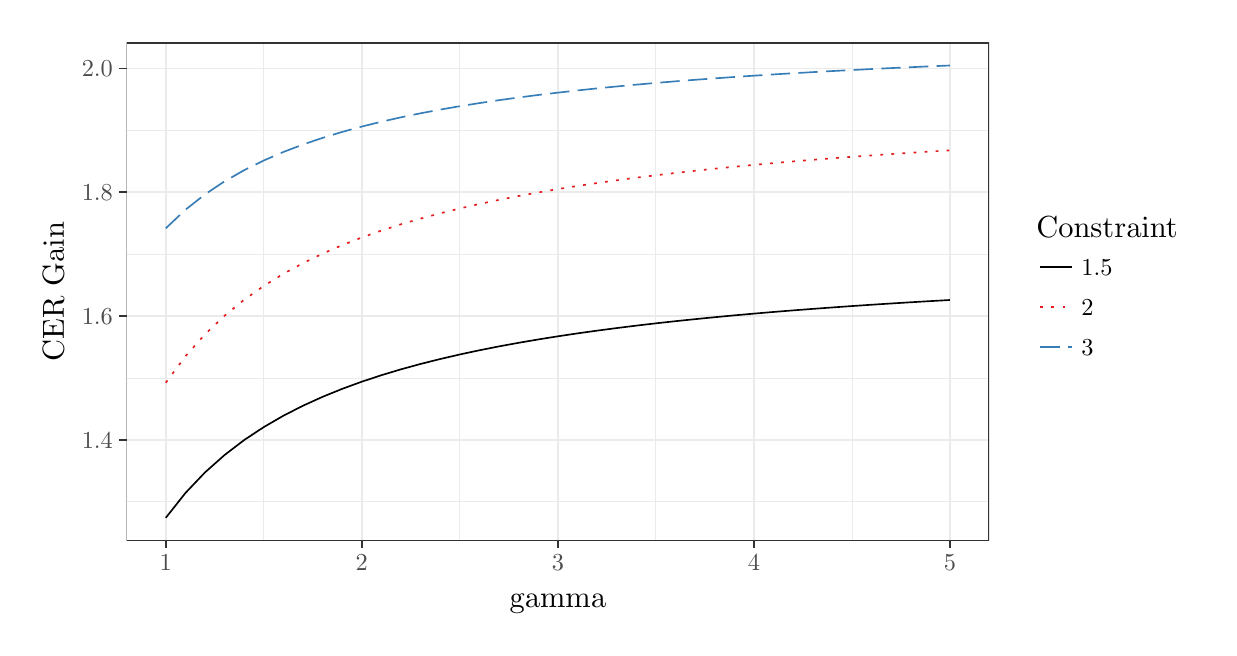
\begin{tikzpicture}[x=1pt,y=1pt]
\definecolor{fillColor}{RGB}{255,255,255}
\path[use as bounding box,fill=fillColor,fill opacity=0.00] (0,0) rectangle (426.79,216.81);
\begin{scope}
\path[clip] (  0.00,  0.00) rectangle (426.79,216.81);
\definecolor{drawColor}{RGB}{255,255,255}
\definecolor{fillColor}{RGB}{255,255,255}

\path[draw=drawColor,line width= 0.6pt,line join=round,line cap=round,fill=fillColor] (  0.00,  0.00) rectangle (426.79,216.81);
\end{scope}
\begin{scope}
\path[clip] ( 35.74, 31.53) rectangle (347.42,211.31);
\definecolor{fillColor}{RGB}{255,255,255}

\path[fill=fillColor] ( 35.74, 31.53) rectangle (347.42,211.31);
\definecolor{drawColor}{gray}{0.92}

\path[draw=drawColor,line width= 0.3pt,line join=round] ( 35.74, 45.51) --
	(347.42, 45.51);

\path[draw=drawColor,line width= 0.3pt,line join=round] ( 35.74, 90.23) --
	(347.42, 90.23);

\path[draw=drawColor,line width= 0.3pt,line join=round] ( 35.74,134.95) --
	(347.42,134.95);

\path[draw=drawColor,line width= 0.3pt,line join=round] ( 35.74,179.67) --
	(347.42,179.67);

\path[draw=drawColor,line width= 0.3pt,line join=round] ( 85.33, 31.53) --
	( 85.33,211.31);

\path[draw=drawColor,line width= 0.3pt,line join=round] (156.16, 31.53) --
	(156.16,211.31);

\path[draw=drawColor,line width= 0.3pt,line join=round] (227.00, 31.53) --
	(227.00,211.31);

\path[draw=drawColor,line width= 0.3pt,line join=round] (297.84, 31.53) --
	(297.84,211.31);

\path[draw=drawColor,line width= 0.6pt,line join=round] ( 35.74, 67.87) --
	(347.42, 67.87);

\path[draw=drawColor,line width= 0.6pt,line join=round] ( 35.74,112.59) --
	(347.42,112.59);

\path[draw=drawColor,line width= 0.6pt,line join=round] ( 35.74,157.31) --
	(347.42,157.31);

\path[draw=drawColor,line width= 0.6pt,line join=round] ( 35.74,202.03) --
	(347.42,202.03);

\path[draw=drawColor,line width= 0.6pt,line join=round] ( 49.91, 31.53) --
	( 49.91,211.31);

\path[draw=drawColor,line width= 0.6pt,line join=round] (120.74, 31.53) --
	(120.74,211.31);

\path[draw=drawColor,line width= 0.6pt,line join=round] (191.58, 31.53) --
	(191.58,211.31);

\path[draw=drawColor,line width= 0.6pt,line join=round] (262.42, 31.53) --
	(262.42,211.31);

\path[draw=drawColor,line width= 0.6pt,line join=round] (333.25, 31.53) --
	(333.25,211.31);
\definecolor{drawColor}{RGB}{0,0,0}

\path[draw=drawColor,line width= 0.6pt,line join=round] ( 49.91, 39.70) --
	( 56.99, 48.65) --
	( 64.07, 56.10) --
	( 71.16, 62.40) --
	( 78.24, 67.81) --
	( 85.33, 72.49) --
	( 92.41, 76.59) --
	( 99.49, 80.21) --
	(106.58, 83.42) --
	(113.66, 86.30) --
	(120.74, 88.89) --
	(127.83, 91.23) --
	(134.91, 93.36) --
	(141.99, 95.30) --
	(149.08, 97.08) --
	(156.16, 98.72) --
	(163.25,100.24) --
	(170.33,101.64) --
	(177.41,102.94) --
	(184.50,104.15) --
	(191.58,105.28) --
	(198.66,106.34) --
	(205.75,107.33) --
	(212.83,108.26) --
	(219.92,109.14) --
	(227.00,109.97) --
	(234.08,110.75) --
	(241.17,111.48) --
	(248.25,112.18) --
	(255.33,112.85) --
	(262.42,113.48) --
	(269.50,114.08) --
	(276.58,114.65) --
	(283.67,115.19) --
	(290.75,115.71) --
	(297.84,116.21) --
	(304.92,116.69) --
	(312.00,117.14) --
	(319.09,117.58) --
	(326.17,118.00) --
	(333.25,118.40);
\definecolor{drawColor}{RGB}{228,26,28}

\path[draw=drawColor,line width= 0.6pt,dash pattern=on 1pt off 3pt ,line join=round] ( 49.91, 88.51) --
	( 56.99, 98.05) --
	( 64.07,106.00) --
	( 71.16,112.73) --
	( 78.24,118.50) --
	( 85.33,123.49) --
	( 92.41,127.87) --
	( 99.49,131.73) --
	(106.58,135.16) --
	(113.66,138.23) --
	(120.74,140.99) --
	(127.83,143.49) --
	(134.91,145.76) --
	(141.99,147.83) --
	(149.08,149.73) --
	(156.16,151.48) --
	(163.25,153.10) --
	(170.33,154.59) --
	(177.41,155.98) --
	(184.50,157.27) --
	(191.58,158.48) --
	(198.66,159.61) --
	(205.75,160.67) --
	(212.83,161.66) --
	(219.92,162.60) --
	(227.00,163.48) --
	(234.08,164.31) --
	(241.17,165.10) --
	(248.25,165.85) --
	(255.33,166.55) --
	(262.42,167.23) --
	(269.50,167.87) --
	(276.58,168.48) --
	(283.67,169.06) --
	(290.75,169.61) --
	(297.84,170.14) --
	(304.92,170.65) --
	(312.00,171.14) --
	(319.09,171.60) --
	(326.17,172.05) --
	(333.25,172.48);
\definecolor{drawColor}{RGB}{55,126,184}

\path[draw=drawColor,line width= 0.6pt,dash pattern=on 7pt off 3pt ,line join=round] ( 49.91,144.31) --
	( 56.99,151.00) --
	( 64.07,156.57) --
	( 71.16,161.28) --
	( 78.24,165.32) --
	( 85.33,168.82) --
	( 92.41,171.89) --
	( 99.49,174.59) --
	(106.58,176.99) --
	(113.66,179.14) --
	(120.74,181.08) --
	(127.83,182.83) --
	(134.91,184.42) --
	(141.99,185.87) --
	(149.08,187.21) --
	(156.16,188.43) --
	(163.25,189.56) --
	(170.33,190.61) --
	(177.41,191.58) --
	(184.50,192.49) --
	(191.58,193.33) --
	(198.66,194.12) --
	(205.75,194.87) --
	(212.83,195.56) --
	(219.92,196.22) --
	(227.00,196.84) --
	(234.08,197.42) --
	(241.17,197.97) --
	(248.25,198.49) --
	(255.33,198.99) --
	(262.42,199.46) --
	(269.50,199.91) --
	(276.58,200.34) --
	(283.67,200.74) --
	(290.75,201.13) --
	(297.84,201.50) --
	(304.92,201.86) --
	(312.00,202.20) --
	(319.09,202.53) --
	(326.17,202.84) --
	(333.25,203.14);
\definecolor{drawColor}{gray}{0.20}

\path[draw=drawColor,line width= 0.6pt,line join=round,line cap=round] ( 35.74, 31.53) rectangle (347.42,211.31);
\end{scope}
\begin{scope}
\path[clip] (  0.00,  0.00) rectangle (426.79,216.81);
\definecolor{drawColor}{gray}{0.30}

\node[text=drawColor,anchor=base east,inner sep=0pt, outer sep=0pt, scale=  0.88] at ( 30.79, 64.84) {1.4};

\node[text=drawColor,anchor=base east,inner sep=0pt, outer sep=0pt, scale=  0.88] at ( 30.79,109.56) {1.6};

\node[text=drawColor,anchor=base east,inner sep=0pt, outer sep=0pt, scale=  0.88] at ( 30.79,154.28) {1.8};

\node[text=drawColor,anchor=base east,inner sep=0pt, outer sep=0pt, scale=  0.88] at ( 30.79,199.00) {2.0};
\end{scope}
\begin{scope}
\path[clip] (  0.00,  0.00) rectangle (426.79,216.81);
\definecolor{drawColor}{gray}{0.20}

\path[draw=drawColor,line width= 0.6pt,line join=round] ( 32.99, 67.87) --
	( 35.74, 67.87);

\path[draw=drawColor,line width= 0.6pt,line join=round] ( 32.99,112.59) --
	( 35.74,112.59);

\path[draw=drawColor,line width= 0.6pt,line join=round] ( 32.99,157.31) --
	( 35.74,157.31);

\path[draw=drawColor,line width= 0.6pt,line join=round] ( 32.99,202.03) --
	( 35.74,202.03);
\end{scope}
\begin{scope}
\path[clip] (  0.00,  0.00) rectangle (426.79,216.81);
\definecolor{drawColor}{gray}{0.20}

\path[draw=drawColor,line width= 0.6pt,line join=round] ( 49.91, 28.78) --
	( 49.91, 31.53);

\path[draw=drawColor,line width= 0.6pt,line join=round] (120.74, 28.78) --
	(120.74, 31.53);

\path[draw=drawColor,line width= 0.6pt,line join=round] (191.58, 28.78) --
	(191.58, 31.53);

\path[draw=drawColor,line width= 0.6pt,line join=round] (262.42, 28.78) --
	(262.42, 31.53);

\path[draw=drawColor,line width= 0.6pt,line join=round] (333.25, 28.78) --
	(333.25, 31.53);
\end{scope}
\begin{scope}
\path[clip] (  0.00,  0.00) rectangle (426.79,216.81);
\definecolor{drawColor}{gray}{0.30}

\node[text=drawColor,anchor=base,inner sep=0pt, outer sep=0pt, scale=  0.88] at ( 49.91, 20.52) {1};

\node[text=drawColor,anchor=base,inner sep=0pt, outer sep=0pt, scale=  0.88] at (120.74, 20.52) {2};

\node[text=drawColor,anchor=base,inner sep=0pt, outer sep=0pt, scale=  0.88] at (191.58, 20.52) {3};

\node[text=drawColor,anchor=base,inner sep=0pt, outer sep=0pt, scale=  0.88] at (262.42, 20.52) {4};

\node[text=drawColor,anchor=base,inner sep=0pt, outer sep=0pt, scale=  0.88] at (333.25, 20.52) {5};
\end{scope}
\begin{scope}
\path[clip] (  0.00,  0.00) rectangle (426.79,216.81);
\definecolor{drawColor}{RGB}{0,0,0}

\node[text=drawColor,anchor=base,inner sep=0pt, outer sep=0pt, scale=  1.10] at (191.58,  7.44) {gamma};
\end{scope}
\begin{scope}
\path[clip] (  0.00,  0.00) rectangle (426.79,216.81);
\definecolor{drawColor}{RGB}{0,0,0}

\node[text=drawColor,rotate= 90.00,anchor=base,inner sep=0pt, outer sep=0pt, scale=  1.10] at ( 13.08,121.42) {CER Gain};
\end{scope}
\begin{scope}
\path[clip] (  0.00,  0.00) rectangle (426.79,216.81);
\definecolor{fillColor}{RGB}{255,255,255}

\path[fill=fillColor] (358.80, 88.45) rectangle (421.29,154.39);
\end{scope}
\begin{scope}
\path[clip] (  0.00,  0.00) rectangle (426.79,216.81);
\definecolor{drawColor}{RGB}{0,0,0}

\node[text=drawColor,anchor=base west,inner sep=0pt, outer sep=0pt, scale=  1.10] at (364.49,141.12) {Constraint};
\end{scope}
\begin{scope}
\path[clip] (  0.00,  0.00) rectangle (426.79,216.81);
\definecolor{fillColor}{RGB}{255,255,255}

\path[fill=fillColor] (364.49,123.05) rectangle (378.95,137.51);
\end{scope}
\begin{scope}
\path[clip] (  0.00,  0.00) rectangle (426.79,216.81);
\definecolor{drawColor}{RGB}{0,0,0}

\path[draw=drawColor,line width= 0.6pt,line join=round] (365.94,130.28) -- (377.50,130.28);
\end{scope}
\begin{scope}
\path[clip] (  0.00,  0.00) rectangle (426.79,216.81);
\definecolor{fillColor}{RGB}{255,255,255}

\path[fill=fillColor] (364.49,108.60) rectangle (378.95,123.05);
\end{scope}
\begin{scope}
\path[clip] (  0.00,  0.00) rectangle (426.79,216.81);
\definecolor{drawColor}{RGB}{228,26,28}

\path[draw=drawColor,line width= 0.6pt,dash pattern=on 1pt off 3pt ,line join=round] (365.94,115.83) -- (377.50,115.83);
\end{scope}
\begin{scope}
\path[clip] (  0.00,  0.00) rectangle (426.79,216.81);
\definecolor{fillColor}{RGB}{255,255,255}

\path[fill=fillColor] (364.49, 94.14) rectangle (378.95,108.60);
\end{scope}
\begin{scope}
\path[clip] (  0.00,  0.00) rectangle (426.79,216.81);
\definecolor{drawColor}{RGB}{55,126,184}

\path[draw=drawColor,line width= 0.6pt,dash pattern=on 7pt off 3pt ,line join=round] (365.94,101.37) -- (377.50,101.37);
\end{scope}
\begin{scope}
\path[clip] (  0.00,  0.00) rectangle (426.79,216.81);
\definecolor{drawColor}{RGB}{0,0,0}

\node[text=drawColor,anchor=base west,inner sep=0pt, outer sep=0pt, scale=  0.88] at (380.75,127.25) {1.5};
\end{scope}
\begin{scope}
\path[clip] (  0.00,  0.00) rectangle (426.79,216.81);
\definecolor{drawColor}{RGB}{0,0,0}

\node[text=drawColor,anchor=base west,inner sep=0pt, outer sep=0pt, scale=  0.88] at (380.75,112.80) {2};
\end{scope}
\begin{scope}
\path[clip] (  0.00,  0.00) rectangle (426.79,216.81);
\definecolor{drawColor}{RGB}{0,0,0}

\node[text=drawColor,anchor=base west,inner sep=0pt, outer sep=0pt, scale=  0.88] at (380.75, 98.34) {3};
\end{scope}
\end{tikzpicture}

	\end{adjustbox}
\end{frame}

\begin{frame}{Leverage}
	\begin{adjustbox}{width=\textwidth}
		% Created by tikzDevice version 0.10.1 on 2018-06-14 11:50:00
% !TEX encoding = UTF-8 Unicode
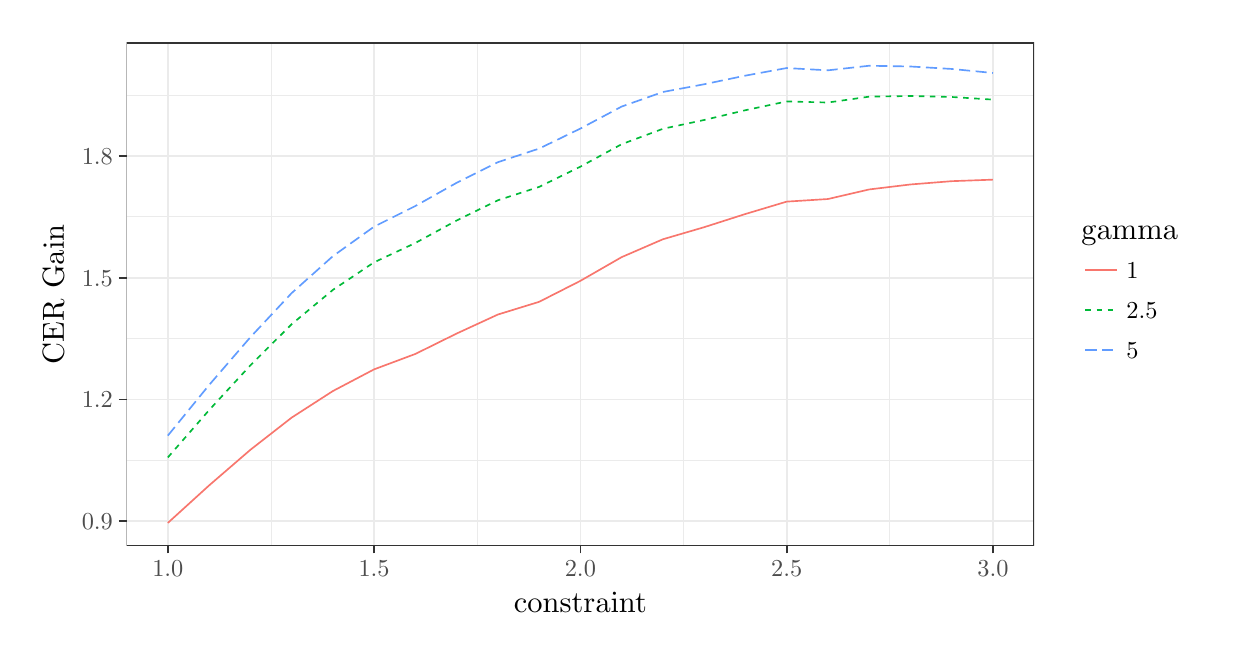
\begin{tikzpicture}[x=1pt,y=1pt]
\definecolor{fillColor}{RGB}{255,255,255}
\path[use as bounding box,fill=fillColor,fill opacity=0.00] (0,0) rectangle (426.79,216.81);
\begin{scope}
\path[clip] (  0.00,  0.00) rectangle (426.79,216.81);
\definecolor{drawColor}{RGB}{255,255,255}
\definecolor{fillColor}{RGB}{255,255,255}

\path[draw=drawColor,line width= 0.6pt,line join=round,line cap=round,fill=fillColor] (  0.00,  0.00) rectangle (426.79,216.81);
\end{scope}
\begin{scope}
\path[clip] ( 35.74, 29.59) rectangle (363.70,211.31);
\definecolor{fillColor}{RGB}{255,255,255}

\path[fill=fillColor] ( 35.74, 29.59) rectangle (363.70,211.31);
\definecolor{drawColor}{gray}{0.92}

\path[draw=drawColor,line width= 0.3pt,line join=round] ( 35.74, 60.51) --
	(363.70, 60.51);

\path[draw=drawColor,line width= 0.3pt,line join=round] ( 35.74,104.47) --
	(363.70,104.47);

\path[draw=drawColor,line width= 0.3pt,line join=round] ( 35.74,148.43) --
	(363.70,148.43);

\path[draw=drawColor,line width= 0.3pt,line join=round] ( 35.74,192.39) --
	(363.70,192.39);

\path[draw=drawColor,line width= 0.3pt,line join=round] ( 87.92, 29.59) --
	( 87.92,211.31);

\path[draw=drawColor,line width= 0.3pt,line join=round] (162.45, 29.59) --
	(162.45,211.31);

\path[draw=drawColor,line width= 0.3pt,line join=round] (236.99, 29.59) --
	(236.99,211.31);

\path[draw=drawColor,line width= 0.3pt,line join=round] (311.53, 29.59) --
	(311.53,211.31);

\path[draw=drawColor,line width= 0.6pt,line join=round] ( 35.74, 38.53) --
	(363.70, 38.53);

\path[draw=drawColor,line width= 0.6pt,line join=round] ( 35.74, 82.49) --
	(363.70, 82.49);

\path[draw=drawColor,line width= 0.6pt,line join=round] ( 35.74,126.45) --
	(363.70,126.45);

\path[draw=drawColor,line width= 0.6pt,line join=round] ( 35.74,170.41) --
	(363.70,170.41);

\path[draw=drawColor,line width= 0.6pt,line join=round] ( 50.65, 29.59) --
	( 50.65,211.31);

\path[draw=drawColor,line width= 0.6pt,line join=round] (125.18, 29.59) --
	(125.18,211.31);

\path[draw=drawColor,line width= 0.6pt,line join=round] (199.72, 29.59) --
	(199.72,211.31);

\path[draw=drawColor,line width= 0.6pt,line join=round] (274.26, 29.59) --
	(274.26,211.31);

\path[draw=drawColor,line width= 0.6pt,line join=round] (348.80, 29.59) --
	(348.80,211.31);
\definecolor{drawColor}{RGB}{248,118,109}

\path[draw=drawColor,line width= 0.6pt,line join=round] ( 50.65, 37.85) --
	( 65.55, 51.39) --
	( 80.46, 64.26) --
	( 95.37, 75.89) --
	(110.28, 85.50) --
	(125.18, 93.34) --
	(140.09, 98.91) --
	(155.00,106.28) --
	(169.91,113.15) --
	(184.81,117.74) --
	(199.72,125.32) --
	(214.63,133.89) --
	(229.54,140.35) --
	(244.44,144.71) --
	(259.35,149.48) --
	(274.26,153.95) --
	(289.17,154.89) --
	(304.07,158.35) --
	(318.98,160.15) --
	(333.89,161.34) --
	(348.80,161.89);
\definecolor{drawColor}{RGB}{0,186,56}

\path[draw=drawColor,line width= 0.6pt,dash pattern=on 2pt off 2pt ,line join=round] ( 50.65, 61.51) --
	( 65.55, 78.60) --
	( 80.46, 94.77) --
	( 95.37,109.64) --
	(110.28,122.05) --
	(125.18,132.02) --
	(140.09,139.01) --
	(155.00,147.13) --
	(169.91,154.44) --
	(184.81,159.27) --
	(199.72,166.59) --
	(214.63,174.70) --
	(229.54,180.27) --
	(244.44,183.45) --
	(259.35,186.98) --
	(274.26,190.15) --
	(289.17,189.76) --
	(304.07,191.88) --
	(318.98,192.12) --
	(333.89,191.76) --
	(348.80,190.81);
\definecolor{drawColor}{RGB}{97,156,255}

\path[draw=drawColor,line width= 0.6pt,dash pattern=on 4pt off 2pt ,line join=round] ( 50.65, 69.40) --
	( 65.55, 87.67) --
	( 80.46,104.94) --
	( 95.37,120.88) --
	(110.28,134.24) --
	(125.18,144.91) --
	(140.09,152.37) --
	(155.00,160.75) --
	(169.91,168.21) --
	(184.81,173.11) --
	(199.72,180.35) --
	(214.63,188.30) --
	(229.54,193.57) --
	(244.44,196.36) --
	(259.35,199.48) --
	(274.26,202.22) --
	(289.17,201.39) --
	(304.07,203.05) --
	(318.98,202.78) --
	(333.89,201.89) --
	(348.80,200.44);
\definecolor{drawColor}{gray}{0.20}

\path[draw=drawColor,line width= 0.6pt,line join=round,line cap=round] ( 35.74, 29.59) rectangle (363.70,211.31);
\end{scope}
\begin{scope}
\path[clip] (  0.00,  0.00) rectangle (426.79,216.81);
\definecolor{drawColor}{gray}{0.30}

\node[text=drawColor,anchor=base east,inner sep=0pt, outer sep=0pt, scale=  0.88] at ( 30.79, 35.50) {0.9};

\node[text=drawColor,anchor=base east,inner sep=0pt, outer sep=0pt, scale=  0.88] at ( 30.79, 79.46) {1.2};

\node[text=drawColor,anchor=base east,inner sep=0pt, outer sep=0pt, scale=  0.88] at ( 30.79,123.42) {1.5};

\node[text=drawColor,anchor=base east,inner sep=0pt, outer sep=0pt, scale=  0.88] at ( 30.79,167.38) {1.8};
\end{scope}
\begin{scope}
\path[clip] (  0.00,  0.00) rectangle (426.79,216.81);
\definecolor{drawColor}{gray}{0.20}

\path[draw=drawColor,line width= 0.6pt,line join=round] ( 32.99, 38.53) --
	( 35.74, 38.53);

\path[draw=drawColor,line width= 0.6pt,line join=round] ( 32.99, 82.49) --
	( 35.74, 82.49);

\path[draw=drawColor,line width= 0.6pt,line join=round] ( 32.99,126.45) --
	( 35.74,126.45);

\path[draw=drawColor,line width= 0.6pt,line join=round] ( 32.99,170.41) --
	( 35.74,170.41);
\end{scope}
\begin{scope}
\path[clip] (  0.00,  0.00) rectangle (426.79,216.81);
\definecolor{drawColor}{gray}{0.20}

\path[draw=drawColor,line width= 0.6pt,line join=round] ( 50.65, 26.84) --
	( 50.65, 29.59);

\path[draw=drawColor,line width= 0.6pt,line join=round] (125.18, 26.84) --
	(125.18, 29.59);

\path[draw=drawColor,line width= 0.6pt,line join=round] (199.72, 26.84) --
	(199.72, 29.59);

\path[draw=drawColor,line width= 0.6pt,line join=round] (274.26, 26.84) --
	(274.26, 29.59);

\path[draw=drawColor,line width= 0.6pt,line join=round] (348.80, 26.84) --
	(348.80, 29.59);
\end{scope}
\begin{scope}
\path[clip] (  0.00,  0.00) rectangle (426.79,216.81);
\definecolor{drawColor}{gray}{0.30}

\node[text=drawColor,anchor=base,inner sep=0pt, outer sep=0pt, scale=  0.88] at ( 50.65, 18.58) {1.0};

\node[text=drawColor,anchor=base,inner sep=0pt, outer sep=0pt, scale=  0.88] at (125.18, 18.58) {1.5};

\node[text=drawColor,anchor=base,inner sep=0pt, outer sep=0pt, scale=  0.88] at (199.72, 18.58) {2.0};

\node[text=drawColor,anchor=base,inner sep=0pt, outer sep=0pt, scale=  0.88] at (274.26, 18.58) {2.5};

\node[text=drawColor,anchor=base,inner sep=0pt, outer sep=0pt, scale=  0.88] at (348.80, 18.58) {3.0};
\end{scope}
\begin{scope}
\path[clip] (  0.00,  0.00) rectangle (426.79,216.81);
\definecolor{drawColor}{RGB}{0,0,0}

\node[text=drawColor,anchor=base,inner sep=0pt, outer sep=0pt, scale=  1.10] at (199.72,  5.50) {constraint};
\end{scope}
\begin{scope}
\path[clip] (  0.00,  0.00) rectangle (426.79,216.81);
\definecolor{drawColor}{RGB}{0,0,0}

\node[text=drawColor,rotate= 90.00,anchor=base,inner sep=0pt, outer sep=0pt, scale=  1.10] at ( 13.08,120.45) {CER Gain};
\end{scope}
\begin{scope}
\path[clip] (  0.00,  0.00) rectangle (426.79,216.81);
\definecolor{fillColor}{RGB}{255,255,255}

\path[fill=fillColor] (375.09, 87.48) rectangle (421.29,153.41);
\end{scope}
\begin{scope}
\path[clip] (  0.00,  0.00) rectangle (426.79,216.81);
\definecolor{drawColor}{RGB}{0,0,0}

\node[text=drawColor,anchor=base west,inner sep=0pt, outer sep=0pt, scale=  1.10] at (380.78,140.15) {gamma};
\end{scope}
\begin{scope}
\path[clip] (  0.00,  0.00) rectangle (426.79,216.81);
\definecolor{fillColor}{RGB}{255,255,255}

\path[fill=fillColor] (380.78,122.08) rectangle (395.23,136.53);
\end{scope}
\begin{scope}
\path[clip] (  0.00,  0.00) rectangle (426.79,216.81);
\definecolor{drawColor}{RGB}{248,118,109}

\path[draw=drawColor,line width= 0.6pt,line join=round] (382.22,129.31) -- (393.78,129.31);
\end{scope}
\begin{scope}
\path[clip] (  0.00,  0.00) rectangle (426.79,216.81);
\definecolor{fillColor}{RGB}{255,255,255}

\path[fill=fillColor] (380.78,107.63) rectangle (395.23,122.08);
\end{scope}
\begin{scope}
\path[clip] (  0.00,  0.00) rectangle (426.79,216.81);
\definecolor{drawColor}{RGB}{0,186,56}

\path[draw=drawColor,line width= 0.6pt,dash pattern=on 2pt off 2pt ,line join=round] (382.22,114.85) -- (393.78,114.85);
\end{scope}
\begin{scope}
\path[clip] (  0.00,  0.00) rectangle (426.79,216.81);
\definecolor{fillColor}{RGB}{255,255,255}

\path[fill=fillColor] (380.78, 93.17) rectangle (395.23,107.63);
\end{scope}
\begin{scope}
\path[clip] (  0.00,  0.00) rectangle (426.79,216.81);
\definecolor{drawColor}{RGB}{97,156,255}

\path[draw=drawColor,line width= 0.6pt,dash pattern=on 4pt off 2pt ,line join=round] (382.22,100.40) -- (393.78,100.40);
\end{scope}
\begin{scope}
\path[clip] (  0.00,  0.00) rectangle (426.79,216.81);
\definecolor{drawColor}{RGB}{0,0,0}

\node[text=drawColor,anchor=base west,inner sep=0pt, outer sep=0pt, scale=  0.88] at (397.04,126.28) {1};
\end{scope}
\begin{scope}
\path[clip] (  0.00,  0.00) rectangle (426.79,216.81);
\definecolor{drawColor}{RGB}{0,0,0}

\node[text=drawColor,anchor=base west,inner sep=0pt, outer sep=0pt, scale=  0.88] at (397.04,111.82) {2.5};
\end{scope}
\begin{scope}
\path[clip] (  0.00,  0.00) rectangle (426.79,216.81);
\definecolor{drawColor}{RGB}{0,0,0}

\node[text=drawColor,anchor=base west,inner sep=0pt, outer sep=0pt, scale=  0.88] at (397.04, 97.37) {5};
\end{scope}
\end{tikzpicture}

	\end{adjustbox}
\end{frame}

%\section{Explaination}
%\begin{frame}{Risk over Reward}
%	\begin{itemize}[<+->]
%		\item The higher excess returns of low-risk strategies (assets) comes from a preference for the lottery like extreme returns possible from higher risk investments - Barberis and Huang (2008); Brunnermeier, Gollier, and Parker (2007); Asness, Frazzini, Gorsmen, Pedersen (2016)
%		\item Leverage constraints prevent investors from taking the low-risk position - Black (1972)
%	\end{itemize}
%\end{frame}

%\begin{frame}{Lottery}
%	\begin{itemize}[<+->]
%		\item For lotter preferences to explain the higher returns of either SV or AV, the Buy and Hold strategy must be more lottery-like than either
%		\item It is not
%		\item 	\begin{adjustbox}{width=\textwidth}
%			
% Table created by stargazer v.5.2 by Marek Hlavac, Harvard University. E-mail: hlavac at fas.harvard.edu
% Date and time: Wed, Mar 28, 2018 - 01:54:14  IST
\begin{table}[!htbp] \centering 
  \caption{} 
  \label{} 
\begin{tabular}{@{\extracolsep{5pt}} cccccccccc} 
\\[-1.8ex]\hline 
\hline \\[-1.8ex] 
 & Strategy & Mean & Median & Sd & KS & Mean\_s & Median\_s & Sd\_s & KS\_s \\ 
\hline \\[-1.8ex] 
1 & BH & $1.776$ & $1.422$ & $1.398$ & $$ & $2.186$ & $1.971$ & $1.046$ & $$ \\ 
2 & SV & $1.569$ & $1.258$ & $1.243$ & $0.539$ & $3.229$ & $2.167$ & $4.661$ & $0$ \\ 
3 & AV & $1.796$ & $1.650$ & $0.960$ & $0$ & $2.884$ & $1.691$ & $4.992$ & $0$ \\ 
4 & BH & $1.134$ & $0.922$ & $0.774$ & $$ & $1.410$ & $1.341$ & $0.540$ & $$ \\ 
5 & SV & $1.023$ & $0.842$ & $0.787$ & $0.393$ & $2.084$ & $1.377$ & $2.765$ & $0$ \\ 
6 & AV & $1.164$ & $1.088$ & $0.534$ & $0$ & $1.827$ & $1.121$ & $2.833$ & $0$ \\ 
\hline \\[-1.8ex] 
\end{tabular} 
\end{table} 

%		\end{adjustbox}
%	\end{itemize}
%\end{frame}
%
%\begin{frame}{Lottery Pick 2}
%		\begin{equation}
%		R^{AV}_{t} = \alpha_{t} + \beta^{1}_{t} R^{M}_{t} + \beta^{2}_{t} R^{M}_{t}*x_{1} + \boldsymbol{\beta}_{t}\boldsymbol{\chi}_{t}
%		\end{equation}
%		\begin{adjustbox}{width=\textwidth,height=4cm}
%			
% Table created by stargazer v.5.2 by Marek Hlavac, Harvard University. E-mail: hlavac at fas.harvard.edu
% Date and time: Sun, Apr 01, 2018 - 12:26:24  IST
\begin{table}[!htbp] \centering 
  \caption{} 
  \label{} 
\begin{tabular}{@{\extracolsep{5pt}}lcccc} 
\\[-1.8ex]\hline 
\hline \\[-1.8ex] 
 & \multicolumn{4}{c}{\textit{Dependent variable:}} \\ 
\cline{2-5} 
\\[-1.8ex] & \multicolumn{4}{c}{av\_mang} \\ 
\\[-1.8ex] & (1) & (2) & (3) & (4)\\ 
\hline \\[-1.8ex] 
 market & 0.880$^{***}$ & 0.939$^{***}$ & 0.880$^{***}$ & 0.940$^{***}$ \\ 
  & (0.027) & (0.027) & (0.030) & (0.029) \\ 
  & & & & \\ 
 gaming\_mcap & 0.000 & 0.000 &  &  \\ 
  & (0.000) & (0.000) &  &  \\ 
  & & & & \\ 
 gratio &  &  & 0.524 & 0.660 \\ 
  &  &  & (0.998) & (0.948) \\ 
  & & & & \\ 
 SMB & 0.023 & 0.080$^{**}$ & 0.022 & 0.081$^{**}$ \\ 
  & (0.035) & (0.036) & (0.035) & (0.036) \\ 
  & & & & \\ 
 HML & 0.024 & $-$0.162$^{***}$ & 0.022 & $-$0.163$^{***}$ \\ 
  & (0.037) & (0.047) & (0.037) & (0.047) \\ 
  & & & & \\ 
 RMW &  & 0.003$^{***}$ &  & 0.003$^{***}$ \\ 
  &  & (0.0005) &  & (0.0005) \\ 
  & & & & \\ 
 CMA &  & 0.004$^{***}$ &  & 0.004$^{***}$ \\ 
  &  & (0.001) &  & (0.001) \\ 
  & & & & \\ 
 market:gaming\_mcap & $-$0.000 & $-$0.000 &  &  \\ 
  & (0.000) & (0.000) &  &  \\ 
  & & & & \\ 
 market:gratio &  &  & $-$18.636 & $-$15.823 \\ 
  &  &  & (24.213) & (22.993) \\ 
  & & & & \\ 
 Constant & 0.002$^{*}$ & 0.0004 & 0.002$^{*}$ & 0.0003 \\ 
  & (0.001) & (0.001) & (0.001) & (0.001) \\ 
  & & & & \\ 
\hline \\[-1.8ex] 
Observations & 525 & 525 & 525 & 525 \\ 
R$^{2}$ & 0.749 & 0.775 & 0.749 & 0.775 \\ 
Adjusted R$^{2}$ & 0.747 & 0.772 & 0.747 & 0.772 \\ 
Residual Std. Error & 0.023 (df = 519) & 0.022 (df = 517) & 0.023 (df = 519) & 0.022 (df = 517) \\ 
F Statistic & 310.474$^{***}$ (df = 5; 519) & 254.386$^{***}$ (df = 7; 517) & 309.913$^{***}$ (df = 5; 519) & 253.995$^{***}$ (df = 7; 517) \\ 
\hline 
\hline \\[-1.8ex] 
\textit{Note:}  & \multicolumn{4}{r}{$^{*}$p$<$0.1; $^{**}$p$<$0.05; $^{***}$p$<$0.01} \\ 
\end{tabular} 
\end{table} 

%		\end{adjustbox}
%\end{frame}
%
%\begin{frame}{Performance Issues}
%	\begin{adjustbox}{width=\textwidth}
%		
% Table created by stargazer v.5.2 by Marek Hlavac, Harvard University. E-mail: hlavac at fas.harvard.edu
% Date and time: Sun, Apr 01, 2018 - 03:05:39  IST
\begin{table}[!htbp] \centering 
  \caption{} 
  \label{} 
\begin{tabular}{@{\extracolsep{5pt}} cccccccc} 
\\[-1.8ex]\hline 
\hline \\[-1.8ex] 
 & Strategy & RET & Sharpe & Sortino & Kappa & UpsidePotential & Rachev \\ 
\hline \\[-1.8ex] 
1 & BH & 5.932 & 0.319 & 0.447 & 0.082 & 0.584 & 0.841 \\ 
2 & SV & 6.171 & 0.467 & 0.691 & 0.128 & 0.667 & 0.982\textasteriskcentered \textasteriskcentered \textasteriskcentered  \\ 
3 & AV & 7.885\textasteriskcentered \textasteriskcentered \textasteriskcentered  & 0.486\textasteriskcentered \textasteriskcentered \textasteriskcentered  & 0.706\textasteriskcentered \textasteriskcentered \textasteriskcentered  & 0.133\textasteriskcentered \textasteriskcentered \textasteriskcentered  & 0.683\textasteriskcentered \textasteriskcentered \textasteriskcentered  & 0.896 \\ 
4 & BH & 5.932 & 0.319 & 0.447 & 0.082 & 0.584 & 0.841 \\ 
5 & SV & 4.649 & 0.433 & 0.619 & 0.113 & 0.646 & 0.897\textasteriskcentered \textasteriskcentered \textasteriskcentered  \\ 
6 & AV & 5.814\textasteriskcentered \textasteriskcentered \textasteriskcentered  & 0.447 & 0.632\textasteriskcentered \textasteriskcentered \textasteriskcentered  & 0.117\textasteriskcentered \textasteriskcentered \textasteriskcentered  & 0.657\textasteriskcentered \textasteriskcentered \textasteriskcentered  & 0.845 \\ 
\hline \\[-1.8ex] 
\end{tabular} 
\end{table} 

%	\end{adjustbox}
%\end{frame}
%
%\begin{frame}{Leverage}
%	\begin{adjustbox}{width=\textwidth,height=4cm}
%		
% Table created by stargazer v.5.2 by Marek Hlavac, Harvard University. E-mail* hlavac at fas.harvard.edu
% Date and time* Sun, Apr 01, 2018 - 03*56*26  IST
%\begin{table}[!htbp] \centering 
%  \caption{} 
%  \label{} 
\begin{tabular}{@{\extracolsep{5pt}}lcccccccc} 
\\[-1.8ex]\hline 
\hline \\[-1.8ex] 
% & \multicolumn{8}{c}{\textit{Dependent variable*}} \\ 
%\cline{2-9} 
\\[-1.8ex] & \multicolumn{8}{c}{AV} \\ 
%\\[-1.8ex] & (1) & (2) & (3) & (4) & (5) & (6) & (7) & (8)\\ 
\hline \\[-1.8ex] 
 BH & 0.724$^{***}$ & 0.805$^{***}$ & 0.788$^{***}$ & 0.843$^{***}$ & 0.804$^{***}$ & 0.889$^{***}$ & 0.858$^{***}$ & 0.900$^{***}$ \\ 
  & (0.027) & (0.029) & (0.042) & (0.041) & (0.033) & (0.035) & (0.025) & (0.026) \\ 
  & & & & & & & & \\ 
 LF$_{AEM}$ & 0.178$^{***}$ & 0.134$^{***}$ &  &  &  &  &  &  \\ 
  & (0.038) & (0.037) &  &  &  &  &  &  \\ 
  & & & & & & & & \\ 
  BH*LF$_{AEM}$ & 1.231$^{***}$ & 1.508$^{***}$ &  &  &  &  &  &  \\ 
  & (0.352) & (0.341) &  &  &  &  &  &  \\ 
  & & & & & & & & \\ 
 ICRF &  &  & 0.0004 & 0.006 &  &  &  &  \\ 
  &  &  & (0.026) & (0.025) &  &  &  &  \\ 
  & & & & & & & & \\ 
   BH*ICRF &  &  & 0.301 & 0.308 &  &  &  &  \\ 
   &  &  & (0.196) & (0.188) &  &  &  &  \\ 
   & & & & & & & & \\ 
 BC &  &  &  &  & $-$0.0002 & $-$0.0001 &  &  \\ 
  &  &  &  &  & (0.0002) & (0.0002) &  &  \\ 
  & & & & & & & & \\ 
   BH*BC &  &  &  &  & 0.001 & $-$0.003 &  &  \\ 
   &  &  &  &  & (0.004) & (0.004) &  &  \\ 
   & & & & & & & & \\ 
 $\Delta$ MD$_{1984}$ &  &  &  &  &  &  & 0.00000 & 0.00000 \\ 
  &  &  &  &  &  &  & (0.00000) & (0.00000) \\ 
  & & & & & & & & \\ 
  BH*$\Delta$ MD$_{1984}$ &  &  &  &  &  &  & 0.00002$^{***}$ & 0.00002$^{***}$ \\ 
  &  &  &  &  &  &  & (0.00000) & (0.00000) \\ 
  & & & & & & & & \\ 
% SMB & $-$0.007 & 0.070$^{*}$ & $-$0.009 & 0.062 & $-$0.015 & 0.051 & $-$0.004 & 0.059 \\ 
%  & (0.036) & (0.039) & (0.038) & (0.040) & (0.037) & (0.040) & (0.035) & (0.037) \\ 
%  & & & & & & & & \\ 
% HML & $-$0.153$^{***}$ & $-$0.241$^{***}$ & $-$0.007 & $-$0.153$^{***}$ & 0.004 & $-$0.164$^{***}$ & 0.037 & $-$0.096$^{**}$ \\ 
%  & (0.053) & (0.058) & (0.041) & (0.052) & (0.040) & (0.052) & (0.036) & (0.047) \\ 
%  & & & & & & & & \\ 
% RMW &  & 0.002$^{***}$ &  & 0.003$^{***}$ &  & 0.003$^{***}$ &  & 0.002$^{***}$ \\ 
%  &  & (0.0005) &  & (0.0005) &  & (0.0005) &  & (0.0005) \\ 
%  & & & & & & & & \\ 
% CMA &  & 0.003$^{***}$ &  & 0.003$^{***}$ &  & 0.003$^{***}$ &  & 0.003$^{***}$ \\ 
%  &  & (0.001) &  & (0.001) &  & (0.001) &  & (0.001) \\ 
%  & & & & & & & & \\ 


 
% Constant & 0.001 & $-$0.001 & 0.002$^{*}$ & 0.0002 & 0.004$^{***}$ & 0.002 & 0.001 & $-$0.001 \\ 
%  & (0.001) & (0.001) & (0.001) & (0.001) & (0.001) & (0.001) & (0.001) & (0.001) \\ 
%  & & & & & & & & \\ 
Controls & FF-3 & FF-5& FF-3 & FF-5& FF-3 & FF-5& FF-3 & FF-5\\
\hline \\[-1.8ex] 
Observations & 396 & 396 & 396 & 396 & 432 & 432 & 431 & 431 \\ 
R$^{2}$ & 0.764 & 0.785 & 0.748 & 0.771 & 0.739 & 0.761 & 0.772 & 0.791 \\ 
Adjusted R$^{2}$ & 0.761 & 0.781 & 0.745 & 0.767 & 0.736 & 0.757 & 0.770 & 0.788 \\ 
%Residual Std. Error & 0.020 (df = 390) & 0.020 (df = 388) & 0.021 (df = 390) & 0.020 (df = 388) & 0.022 (df = 426) & 0.021 (df = 424) & 0.020 (df = 425) & 0.020 (df = 423) \\ 
%F Statistic & 252.600$^{***}$ (df = 5; 390) & 202.425$^{***}$ (df = 7; 388) & 231.430$^{***}$ (df = 5; 390) & 186.549$^{***}$ (df = 7; 388) & 241.132$^{***}$ (df = 5; 426) & 192.947$^{***}$ (df = 7; 424) & 288.605$^{***}$ (df = 5; 425) & 229.297$^{***}$ (df = 7; 423) \\ 
\hline 
\hline \\[-1.8ex] 
\textit{Note*}  & \multicolumn{8}{r}{$^{*}$p$<$0.1; $^{**}$p$<$0.05; $^{***}$p$<$0.01} \\ 
\end{tabular} 
%\end{table} 

%	\end{adjustbox}
%\end{frame}
%
%\begin{frame}{Leverage}
%	\begin{adjustbox}{width=\textwidth,height=4cm}
%		
% Table created by stargazer v.5.2 by Marek Hlavac, Harvard University. E-mail: hlavac at fas.harvard.edu
% Date and time: Sun, Apr 01, 2018 - 03:56:28  IST
\begin{table}[!htbp] \centering 
  \caption{} 
  \label{} 
\begin{tabular}{@{\extracolsep{5pt}}lcccccc} 
\\[-1.8ex]\hline 
\hline \\[-1.8ex] 
 & \multicolumn{6}{c}{\textit{Dependent variable:}} \\ 
\cline{2-7} 
\\[-1.8ex] & \multicolumn{6}{c}{av\_mang} \\ 
\\[-1.8ex] & (1) & (2) & (3) & (4) & (5) & (6)\\ 
\hline \\[-1.8ex] 
 market & 0.596$^{***}$ & 0.675$^{***}$ & 0.445$^{***}$ & 0.619$^{***}$ & 0.561$^{***}$ & 0.661$^{***}$ \\ 
  & (0.065) & (0.065) & (0.097) & (0.102) & (0.075) & (0.075) \\ 
  & & & & & & \\ 
 rate & $-$0.0004 & $-$0.001 &  &  &  &  \\ 
  & (0.0005) & (0.0005) &  &  &  &  \\ 
  & & & & & & \\ 
 call\_money &  &  & 0.00002 & 0.00005 &  &  \\ 
  &  &  & (0.001) & (0.001) &  &  \\ 
  & & & & & & \\ 
 bank\_prime &  &  &  &  & $-$0.001 & $-$0.001 \\ 
  &  &  &  &  & (0.0004) & (0.0004) \\ 
  & & & & & & \\ 
 SMB & 0.017 & 0.089$^{**}$ & 0.027 & 0.092$^{**}$ & 0.008 & 0.077$^{*}$ \\ 
  & (0.042) & (0.045) & (0.039) & (0.042) & (0.040) & (0.042) \\ 
  & & & & & & \\ 
 HML & 0.099$^{**}$ & $-$0.122$^{**}$ & 0.188$^{***}$ & 0.020 & 0.073 & $-$0.115$^{**}$ \\ 
  & (0.049) & (0.059) & (0.048) & (0.063) & (0.045) & (0.055) \\ 
  & & & & & & \\ 
 RMW &  & 0.003$^{***}$ &  & 0.002$^{***}$ &  & 0.003$^{***}$ \\ 
  &  & (0.001) &  & (0.001) &  & (0.001) \\ 
  & & & & & & \\ 
 CMA &  & 0.004$^{***}$ &  & 0.002$^{***}$ &  & 0.003$^{***}$ \\ 
  &  & (0.001) &  & (0.001) &  & (0.001) \\ 
  & & & & & & \\ 
 market:rate & 0.033$^{***}$ & 0.039$^{***}$ &  &  &  &  \\ 
  & (0.012) & (0.012) &  &  &  &  \\ 
  & & & & & & \\ 
 market:call\_money &  &  & 0.061$^{***}$ & 0.044$^{***}$ &  &  \\ 
  &  &  & (0.013) & (0.013) &  &  \\ 
  & & & & & & \\ 
 market:bank\_prime &  &  &  &  & 0.037$^{***}$ & 0.033$^{***}$ \\ 
  &  &  &  &  & (0.011) & (0.010) \\ 
  & & & & & & \\ 
 Constant & 0.006$^{**}$ & 0.004$^{*}$ & 0.001 & $-$0.0003 & 0.007$^{**}$ & 0.005$^{*}$ \\ 
  & (0.003) & (0.003) & (0.004) & (0.004) & (0.003) & (0.003) \\ 
  & & & & & & \\ 
\hline \\[-1.8ex] 
Observations & 336 & 336 & 265 & 265 & 395 & 395 \\ 
R$^{2}$ & 0.678 & 0.712 & 0.802 & 0.818 & 0.729 & 0.753 \\ 
Adjusted R$^{2}$ & 0.673 & 0.706 & 0.798 & 0.813 & 0.726 & 0.749 \\ 
Residual Std. Error & 0.023 (df = 330) & 0.021 (df = 328) & 0.019 (df = 259) & 0.018 (df = 257) & 0.022 (df = 389) & 0.021 (df = 387) \\ 
F Statistic & 138.711$^{***}$ (df = 5; 330) & 116.012$^{***}$ (df = 7; 328) & 209.909$^{***}$ (df = 5; 259) & 165.276$^{***}$ (df = 7; 257) & 209.268$^{***}$ (df = 5; 389) & 168.702$^{***}$ (df = 7; 387) \\ 
\hline 
\hline \\[-1.8ex] 
\textit{Note:}  & \multicolumn{6}{r}{$^{*}$p$<$0.1; $^{**}$p$<$0.05; $^{***}$p$<$0.01} \\ 
\end{tabular} 
\end{table} 

%	\end{adjustbox}
%\end{frame}
%
%\section{Conclusions}
%\begin{frame}{Conclusions}
%\begin{itemize}[<+->]
%\item Market variation contains average correlation which is compensated by higher returns
%\item SV management throws out return with risk, AV does not
%\item AV out performs in all most all measures
%\item Neither SV nor AV can be expained as behavior, lottery preference stories
%\item Leverage constraints are a better explaination of the returns to SV and AV above the market
%\end{itemize}
%\end{frame}
%
%\begin{frame}{TO DO}
%	\begin{itemize}
%			\item Portfolio performance significance
%			\item Different c adjustments (don't require knowing the BH variance)
%			\item Subsample robust stats - Inoune and Rossi (2012)
%			\item Expand the left hand side - international / portfolio of equity indexes
%			\item AV utility gains
%	\end{itemize}
%
%\end{frame}
%
%\begin{frame}{Time Series}
%	\begin{adjustbox}{width=\textwidth}
%		% Created by tikzDevice version 0.10.1 on 2018-03-26 03:20:57
% !TEX encoding = UTF-8 Unicode
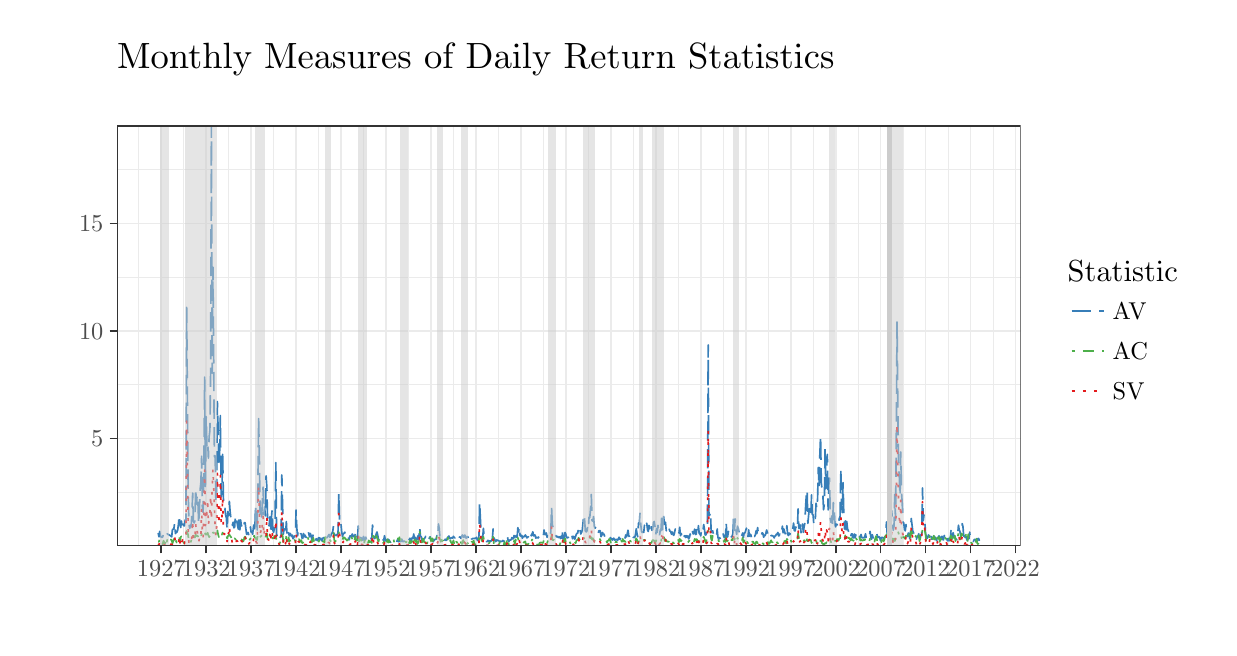
\begin{tikzpicture}[x=1pt,y=1pt]
\definecolor{fillColor}{RGB}{255,255,255}
\path[use as bounding box,fill=fillColor,fill opacity=0.00] (0,0) rectangle (426.79,216.81);
\begin{scope}
\path[clip] (  0.00,  0.00) rectangle (426.79,216.81);
\definecolor{drawColor}{RGB}{255,255,255}
\definecolor{fillColor}{RGB}{255,255,255}

\path[draw=drawColor,line width= 0.6pt,line join=round,line cap=round,fill=fillColor] (  0.00,  0.00) rectangle (426.79,216.81);
\end{scope}
\begin{scope}
\path[clip] ( 32.32, 29.59) rectangle (358.76,181.36);
\definecolor{fillColor}{RGB}{255,255,255}

\path[fill=fillColor] ( 32.32, 29.59) rectangle (358.76,181.36);
\definecolor{drawColor}{gray}{0.92}

\path[draw=drawColor,line width= 0.3pt,line join=round] ( 32.32, 48.97) --
	(358.76, 48.97);

\path[draw=drawColor,line width= 0.3pt,line join=round] ( 32.32, 87.81) --
	(358.76, 87.81);

\path[draw=drawColor,line width= 0.3pt,line join=round] ( 32.32,126.66) --
	(358.76,126.66);

\path[draw=drawColor,line width= 0.3pt,line join=round] ( 32.32,165.51) --
	(358.76,165.51);

\path[draw=drawColor,line width= 0.3pt,line join=round] ( 40.16, 29.59) --
	( 40.16,181.36);

\path[draw=drawColor,line width= 0.3pt,line join=round] ( 56.40, 29.59) --
	( 56.40,181.36);

\path[draw=drawColor,line width= 0.3pt,line join=round] ( 72.65, 29.59) --
	( 72.65,181.36);

\path[draw=drawColor,line width= 0.3pt,line join=round] ( 88.90, 29.59) --
	( 88.90,181.36);

\path[draw=drawColor,line width= 0.3pt,line join=round] (105.14, 29.59) --
	(105.14,181.36);

\path[draw=drawColor,line width= 0.3pt,line join=round] (121.39, 29.59) --
	(121.39,181.36);

\path[draw=drawColor,line width= 0.3pt,line join=round] (137.63, 29.59) --
	(137.63,181.36);

\path[draw=drawColor,line width= 0.3pt,line join=round] (153.88, 29.59) --
	(153.88,181.36);

\path[draw=drawColor,line width= 0.3pt,line join=round] (170.12, 29.59) --
	(170.12,181.36);

\path[draw=drawColor,line width= 0.3pt,line join=round] (186.37, 29.59) --
	(186.37,181.36);

\path[draw=drawColor,line width= 0.3pt,line join=round] (202.62, 29.59) --
	(202.62,181.36);

\path[draw=drawColor,line width= 0.3pt,line join=round] (218.86, 29.59) --
	(218.86,181.36);

\path[draw=drawColor,line width= 0.3pt,line join=round] (235.11, 29.59) --
	(235.11,181.36);

\path[draw=drawColor,line width= 0.3pt,line join=round] (251.35, 29.59) --
	(251.35,181.36);

\path[draw=drawColor,line width= 0.3pt,line join=round] (267.60, 29.59) --
	(267.60,181.36);

\path[draw=drawColor,line width= 0.3pt,line join=round] (283.85, 29.59) --
	(283.85,181.36);

\path[draw=drawColor,line width= 0.3pt,line join=round] (300.09, 29.59) --
	(300.09,181.36);

\path[draw=drawColor,line width= 0.3pt,line join=round] (316.33, 29.59) --
	(316.33,181.36);

\path[draw=drawColor,line width= 0.3pt,line join=round] (332.58, 29.59) --
	(332.58,181.36);

\path[draw=drawColor,line width= 0.3pt,line join=round] (348.83, 29.59) --
	(348.83,181.36);

\path[draw=drawColor,line width= 0.6pt,line join=round] ( 32.32, 68.39) --
	(358.76, 68.39);

\path[draw=drawColor,line width= 0.6pt,line join=round] ( 32.32,107.24) --
	(358.76,107.24);

\path[draw=drawColor,line width= 0.6pt,line join=round] ( 32.32,146.09) --
	(358.76,146.09);

\path[draw=drawColor,line width= 0.6pt,line join=round] ( 48.28, 29.59) --
	( 48.28,181.36);

\path[draw=drawColor,line width= 0.6pt,line join=round] ( 64.53, 29.59) --
	( 64.53,181.36);

\path[draw=drawColor,line width= 0.6pt,line join=round] ( 80.78, 29.59) --
	( 80.78,181.36);

\path[draw=drawColor,line width= 0.6pt,line join=round] ( 97.02, 29.59) --
	( 97.02,181.36);

\path[draw=drawColor,line width= 0.6pt,line join=round] (113.26, 29.59) --
	(113.26,181.36);

\path[draw=drawColor,line width= 0.6pt,line join=round] (129.51, 29.59) --
	(129.51,181.36);

\path[draw=drawColor,line width= 0.6pt,line join=round] (145.76, 29.59) --
	(145.76,181.36);

\path[draw=drawColor,line width= 0.6pt,line join=round] (162.00, 29.59) --
	(162.00,181.36);

\path[draw=drawColor,line width= 0.6pt,line join=round] (178.25, 29.59) --
	(178.25,181.36);

\path[draw=drawColor,line width= 0.6pt,line join=round] (194.49, 29.59) --
	(194.49,181.36);

\path[draw=drawColor,line width= 0.6pt,line join=round] (210.74, 29.59) --
	(210.74,181.36);

\path[draw=drawColor,line width= 0.6pt,line join=round] (226.99, 29.59) --
	(226.99,181.36);

\path[draw=drawColor,line width= 0.6pt,line join=round] (243.23, 29.59) --
	(243.23,181.36);

\path[draw=drawColor,line width= 0.6pt,line join=round] (259.47, 29.59) --
	(259.47,181.36);

\path[draw=drawColor,line width= 0.6pt,line join=round] (275.72, 29.59) --
	(275.72,181.36);

\path[draw=drawColor,line width= 0.6pt,line join=round] (291.97, 29.59) --
	(291.97,181.36);

\path[draw=drawColor,line width= 0.6pt,line join=round] (308.21, 29.59) --
	(308.21,181.36);

\path[draw=drawColor,line width= 0.6pt,line join=round] (324.45, 29.59) --
	(324.45,181.36);

\path[draw=drawColor,line width= 0.6pt,line join=round] (340.71, 29.59) --
	(340.71,181.36);

\path[draw=drawColor,line width= 0.6pt,line join=round] (356.95, 29.59) --
	(356.95,181.36);
\definecolor{drawColor}{RGB}{55,126,184}

\path[draw=drawColor,line width= 0.6pt,dash pattern=on 7pt off 3pt ,line join=round] ( 47.16, 34.17) --
	( 47.44, 32.84) --
	( 47.70, 34.78) --
	( 47.98, 32.86) --
	( 48.25, 32.94) --
	( 48.52, 32.62) --
	( 48.80, 32.80) --
	( 49.05, 33.83) --
	( 49.32, 33.16) --
	( 49.59, 33.11) --
	( 49.87, 33.40) --
	( 50.13, 33.08) --
	( 50.41, 33.91) --
	( 50.68, 33.68) --
	( 50.95, 33.69) --
	( 51.23, 33.38) --
	( 51.49, 33.36) --
	( 51.77, 33.07) --
	( 52.05, 32.83) --
	( 52.30, 35.46) --
	( 52.58, 35.55) --
	( 52.85, 35.87) --
	( 53.12, 37.94) --
	( 53.39, 33.99) --
	( 53.66, 34.55) --
	( 53.94, 34.49) --
	( 54.21, 35.34) --
	( 54.48, 37.37) --
	( 54.75, 40.62) --
	( 55.03, 37.58) --
	( 55.30, 36.21) --
	( 55.55, 38.54) --
	( 55.83, 36.42) --
	( 56.09, 38.23) --
	( 56.37, 36.86) --
	( 56.64, 36.77) --
	( 56.91, 38.91) --
	( 57.19, 38.25) --
	( 57.45,115.74) --
	( 57.73, 80.56) --
	( 58.00, 48.93) --
	( 58.27, 37.47) --
	( 58.55, 35.88) --
	( 58.80, 37.01) --
	( 59.07, 36.49) --
	( 59.34, 40.81) --
	( 59.62, 48.62) --
	( 59.88, 38.72) --
	( 60.16, 37.83) --
	( 60.43, 38.62) --
	( 60.70, 50.30) --
	( 60.98, 44.61) --
	( 61.24, 47.95) --
	( 61.52, 45.64) --
	( 61.79, 37.52) --
	( 62.04, 42.07) --
	( 62.32, 49.97) --
	( 62.59, 52.48) --
	( 62.86, 61.96) --
	( 63.13, 42.31) --
	( 63.40, 41.69) --
	( 63.68, 61.50) --
	( 63.95, 90.55) --
	( 64.22, 51.03) --
	( 64.49, 76.27) --
	( 64.77, 65.88) --
	( 65.04, 67.22) --
	( 65.30, 61.24) --
	( 65.58, 69.11) --
	( 65.84, 71.19) --
	( 66.12, 93.13) --
	( 66.38,181.36) --
	( 66.66, 91.93) --
	( 66.94,130.29) --
	( 67.20, 97.95) --
	( 67.48, 61.76) --
	( 67.75, 62.06) --
	( 68.02, 44.99) --
	( 68.30, 51.26) --
	( 68.55, 81.70) --
	( 68.82, 71.54) --
	( 69.09, 58.86) --
	( 69.36, 63.08) --
	( 69.63, 76.65) --
	( 69.91, 47.31) --
	( 70.18, 49.17) --
	( 70.45, 62.60) --
	( 70.73, 46.62) --
	( 70.99, 43.01) --
	( 71.27, 43.08) --
	( 71.54, 40.63) --
	( 71.79, 39.68) --
	( 72.07, 35.35) --
	( 72.34, 41.99) --
	( 72.61, 40.45) --
	( 72.88, 45.62) --
	( 73.15, 41.98) --
	( 73.43, 39.55) --
	( 73.70, 39.62) --
	( 73.97, 36.96) --
	( 74.24, 38.11) --
	( 74.52, 36.06) --
	( 74.79, 36.39) --
	( 75.04, 40.09) --
	( 75.32, 37.98) --
	( 75.58, 38.54) --
	( 75.86, 36.81) --
	( 76.13, 35.59) --
	( 76.40, 39.19) --
	( 76.68, 35.33) --
	( 76.94, 38.96) --
	( 77.22, 37.00) --
	( 77.49, 36.36) --
	( 77.76, 36.34) --
	( 78.04, 35.60) --
	( 78.30, 37.95) --
	( 78.57, 37.90) --
	( 78.84, 35.77) --
	( 79.11, 33.72) --
	( 79.38, 34.12) --
	( 79.66, 34.38) --
	( 79.93, 33.28) --
	( 80.20, 34.43) --
	( 80.48, 36.42) --
	( 80.74, 34.54) --
	( 81.02, 34.58) --
	( 81.29, 33.74) --
	( 81.54, 36.06) --
	( 81.82, 38.15) --
	( 82.09, 35.73) --
	( 82.36, 44.37) --
	( 82.63, 36.70) --
	( 82.90, 34.21) --
	( 83.18, 50.40) --
	( 83.45, 75.53) --
	( 83.72, 61.64) --
	( 83.99, 41.05) --
	( 84.27, 42.94) --
	( 84.54, 39.77) --
	( 84.79, 45.54) --
	( 85.07, 50.78) --
	( 85.33, 40.90) --
	( 85.61, 43.68) --
	( 85.88, 40.40) --
	( 86.15, 54.89) --
	( 86.43, 50.67) --
	( 86.69, 38.42) --
	( 86.97, 36.54) --
	( 87.24, 36.93) --
	( 87.51, 40.06) --
	( 87.79, 34.47) --
	( 88.04, 39.44) --
	( 88.31, 42.44) --
	( 88.58, 35.29) --
	( 88.86, 34.44) --
	( 89.12, 35.78) --
	( 89.40, 38.87) --
	( 89.67, 59.67) --
	( 89.94, 33.84) --
	( 90.22, 32.84) --
	( 90.48, 33.27) --
	( 90.76, 32.97) --
	( 91.03, 31.80) --
	( 91.29, 32.71) --
	( 91.57, 33.43) --
	( 91.84, 55.19) --
	( 92.11, 44.03) --
	( 92.38, 33.78) --
	( 92.65, 35.69) --
	( 92.93, 35.59) --
	( 93.20, 33.92) --
	( 93.47, 38.34) --
	( 93.74, 32.64) --
	( 94.01, 33.51) --
	( 94.29, 34.36) --
	( 94.54, 33.15) --
	( 94.82, 34.06) --
	( 95.08, 33.69) --
	( 95.36, 32.91) --
	( 95.62, 33.44) --
	( 95.90, 32.11) --
	( 96.18, 32.64) --
	( 96.44, 33.16) --
	( 96.72, 33.12) --
	( 96.99, 42.52) --
	( 97.26, 35.88) --
	( 97.54, 33.18) --
	( 97.79, 35.45) --
	( 98.06, 35.68) --
	( 98.33, 34.67) --
	( 98.60, 34.01) --
	( 98.87, 33.87) --
	( 99.15, 32.36) --
	( 99.42, 32.29) --
	( 99.69, 34.00) --
	( 99.97, 32.87) --
	(100.23, 33.42) --
	(100.51, 32.76) --
	(100.78, 32.61) --
	(101.03, 33.84) --
	(101.31, 35.10) --
	(101.58, 33.95) --
	(101.85, 32.80) --
	(102.12, 34.05) --
	(102.39, 33.37) --
	(102.67, 31.97) --
	(102.94, 32.14) --
	(103.21, 34.17) --
	(103.48, 33.07) --
	(103.76, 31.96) --
	(104.03, 31.70) --
	(104.29, 32.13) --
	(104.56, 31.59) --
	(104.83, 31.43) --
	(105.11, 32.52) --
	(105.37, 32.47) --
	(105.65, 31.90) --
	(105.93, 32.30) --
	(106.19, 31.40) --
	(106.47, 31.44) --
	(106.74, 32.42) --
	(107.01, 32.53) --
	(107.29, 31.66) --
	(107.54, 33.11) --
	(107.81, 32.38) --
	(108.08, 32.46) --
	(108.35, 32.83) --
	(108.62, 33.22) --
	(108.90, 33.69) --
	(109.17, 32.66) --
	(109.44, 32.97) --
	(109.72, 33.84) --
	(109.98, 34.16) --
	(110.26, 34.91) --
	(110.53, 37.01) --
	(110.78, 33.87) --
	(111.06, 33.30) --
	(111.33, 33.50) --
	(111.60, 33.30) --
	(111.87, 33.82) --
	(112.14, 33.83) --
	(112.42, 48.63) --
	(112.69, 39.21) --
	(112.96, 36.54) --
	(113.23, 37.24) --
	(113.50, 34.34) --
	(113.78, 32.99) --
	(114.03, 34.06) --
	(114.31, 34.01) --
	(114.57, 34.51) --
	(114.85, 33.50) --
	(115.11, 33.68) --
	(115.39, 32.30) --
	(115.67, 32.68) --
	(115.93, 32.59) --
	(116.21, 31.76) --
	(116.48, 33.17) --
	(116.75, 33.08) --
	(117.03, 33.09) --
	(117.29, 33.85) --
	(117.56, 32.85) --
	(117.83, 33.32) --
	(118.10, 32.78) --
	(118.37, 33.87) --
	(118.65, 32.26) --
	(118.92, 33.43) --
	(119.19, 32.18) --
	(119.46, 36.76) --
	(119.73, 32.80) --
	(120.01, 32.60) --
	(120.28, 32.50) --
	(120.53, 32.46) --
	(120.81, 31.64) --
	(121.07, 31.81) --
	(121.35, 32.98) --
	(121.62, 31.33) --
	(121.89, 32.00) --
	(122.17, 32.71) --
	(122.44, 31.79) --
	(122.71, 31.90) --
	(122.98, 32.15) --
	(123.25, 32.29) --
	(123.53, 31.34) --
	(123.78, 32.00) --
	(124.05, 32.33) --
	(124.32, 31.76) --
	(124.60, 37.07) --
	(124.86, 35.58) --
	(125.14, 32.36) --
	(125.42, 32.19) --
	(125.68, 32.92) --
	(125.96, 33.92) --
	(126.23, 34.58) --
	(126.50, 33.39) --
	(126.78, 31.72) --
	(127.03, 32.46) --
	(127.30, 31.91) --
	(127.57, 32.48) --
	(127.84, 31.98) --
	(128.11, 32.28) --
	(128.39, 31.81) --
	(128.66, 31.50) --
	(128.93, 33.24) --
	(129.21, 32.00) --
	(129.47, 31.33) --
	(129.75, 31.73) --
	(130.02, 31.81) --
	(130.28, 31.92) --
	(130.56, 31.66) --
	(130.82, 31.23) --
	(131.10, 30.85) --
	(131.37, 30.98) --
	(131.64, 30.73) --
	(131.92, 31.13) --
	(132.19, 31.68) --
	(132.46, 31.19) --
	(132.73, 31.13) --
	(133.00, 31.01) --
	(133.28, 30.91) --
	(133.53, 31.55) --
	(133.80, 31.94) --
	(134.07, 31.04) --
	(134.35, 31.91) --
	(134.61, 31.07) --
	(134.89, 31.12) --
	(135.17, 32.00) --
	(135.43, 31.23) --
	(135.71, 31.03) --
	(135.97, 31.28) --
	(136.25, 31.20) --
	(136.53, 31.09) --
	(136.78, 31.42) --
	(137.05, 31.61) --
	(137.32, 31.37) --
	(137.59, 32.58) --
	(137.86, 31.80) --
	(138.14, 32.32) --
	(138.41, 31.45) --
	(138.68, 31.61) --
	(138.95, 32.52) --
	(139.22, 32.35) --
	(139.50, 33.83) --
	(139.77, 31.86) --
	(140.02, 33.92) --
	(140.30, 31.71) --
	(140.56, 31.92) --
	(140.84, 31.90) --
	(141.11, 33.31) --
	(141.38, 31.88) --
	(141.66, 36.40) --
	(141.93, 32.99) --
	(142.20, 32.93) --
	(142.47, 31.38) --
	(142.74, 31.99) --
	(143.02, 31.81) --
	(143.28, 32.11) --
	(143.55, 32.46) --
	(143.82, 33.02) --
	(144.10, 32.87) --
	(144.36, 31.69) --
	(144.64, 32.09) --
	(144.91, 31.58) --
	(145.18, 32.52) --
	(145.46, 32.83) --
	(145.72, 31.89) --
	(146.00, 31.71) --
	(146.28, 32.08) --
	(146.53, 31.03) --
	(146.80, 31.48) --
	(147.07, 31.88) --
	(147.34, 31.89) --
	(147.61, 31.93) --
	(147.89, 33.30) --
	(148.16, 32.54) --
	(148.43, 37.47) --
	(148.70, 35.86) --
	(148.97, 32.73) --
	(149.25, 32.47) --
	(149.52, 31.61) --
	(149.77, 31.51) --
	(150.05, 31.75) --
	(150.31, 31.34) --
	(150.59, 31.34) --
	(150.86, 31.96) --
	(151.13, 31.57) --
	(151.41, 31.65) --
	(151.68, 32.56) --
	(151.95, 32.81) --
	(152.22, 33.13) --
	(152.49, 32.25) --
	(152.77, 32.09) --
	(153.02, 32.46) --
	(153.29, 32.51) --
	(153.56, 32.37) --
	(153.84, 33.02) --
	(154.10, 32.62) --
	(154.38, 32.43) --
	(154.66, 33.30) --
	(154.92, 32.60) --
	(155.20, 32.43) --
	(155.47, 32.22) --
	(155.74, 32.08) --
	(156.02, 32.72) --
	(156.27, 32.80) --
	(156.55, 32.26) --
	(156.82, 32.99) --
	(157.09, 33.48) --
	(157.36, 32.81) --
	(157.64, 32.64) --
	(157.91, 33.46) --
	(158.18, 33.17) --
	(158.45, 32.32) --
	(158.72, 32.71) --
	(159.00, 32.88) --
	(159.27, 32.31) --
	(159.52, 32.87) --
	(159.80, 33.65) --
	(160.06, 32.65) --
	(160.34, 32.11) --
	(160.61, 32.04) --
	(160.88, 32.28) --
	(161.16, 32.27) --
	(161.43, 32.21) --
	(161.70, 32.38) --
	(161.97, 32.21) --
	(162.24, 32.65) --
	(162.52, 31.54) --
	(162.77, 31.48) --
	(163.04, 32.40) --
	(163.31, 45.35) --
	(163.59, 39.25) --
	(163.85, 33.87) --
	(164.13, 32.42) --
	(164.41, 32.16) --
	(164.67, 35.91) --
	(164.95, 32.74) --
	(165.21, 31.93) --
	(165.49, 31.97) --
	(165.77, 31.14) --
	(166.02, 31.10) --
	(166.29, 31.55) --
	(166.56, 31.37) --
	(166.83, 31.12) --
	(167.10, 31.41) --
	(167.38, 31.29) --
	(167.65, 31.46) --
	(167.92, 32.27) --
	(168.19, 35.72) --
	(168.46, 31.64) --
	(168.74, 32.03) --
	(169.01, 31.08) --
	(169.27, 31.30) --
	(169.55, 31.74) --
	(169.81, 31.42) --
	(170.09, 31.54) --
	(170.36, 31.25) --
	(170.63, 31.26) --
	(170.91, 31.21) --
	(171.17, 31.14) --
	(171.45, 31.24) --
	(171.72, 31.53) --
	(171.99, 31.11) --
	(172.27, 31.29) --
	(172.52, 31.16) --
	(172.79, 31.10) --
	(173.06, 31.23) --
	(173.34, 33.10) --
	(173.60, 31.54) --
	(173.88, 31.16) --
	(174.15, 31.69) --
	(174.42, 31.61) --
	(174.70, 31.78) --
	(174.96, 32.55) --
	(175.24, 32.09) --
	(175.52, 32.13) --
	(175.76, 33.28) --
	(176.04, 32.64) --
	(176.31, 34.89) --
	(176.58, 32.82) --
	(176.85, 32.61) --
	(177.13, 36.14) --
	(177.40, 34.65) --
	(177.67, 36.43) --
	(177.94, 33.17) --
	(178.21, 33.13) --
	(178.49, 33.40) --
	(178.76, 32.31) --
	(179.01, 33.02) --
	(179.29, 32.82) --
	(179.55, 33.02) --
	(179.83, 33.50) --
	(180.10, 33.05) --
	(180.37, 32.46) --
	(180.65, 32.62) --
	(180.92, 32.93) --
	(181.19, 33.85) --
	(181.46, 32.87) --
	(181.73, 33.83) --
	(182.01, 33.17) --
	(182.27, 33.91) --
	(182.54, 34.64) --
	(182.81, 33.17) --
	(183.09, 33.45) --
	(183.35, 33.50) --
	(183.63, 32.37) --
	(183.90, 32.57) --
	(184.17, 32.66) --
	(184.45, 32.40) --
	(184.71, 32.82) --
	(184.99, 33.20) --
	(185.27, 32.39) --
	(185.51, 32.67) --
	(185.79, 32.82) --
	(186.06, 32.72) --
	(186.33, 33.14) --
	(186.60, 35.29) --
	(186.88, 33.65) --
	(187.15, 33.61) --
	(187.42, 34.22) --
	(187.69, 32.64) --
	(187.96, 34.25) --
	(188.24, 34.46) --
	(188.51, 34.83) --
	(188.76, 33.66) --
	(189.04, 34.55) --
	(189.30, 43.59) --
	(189.58, 37.20) --
	(189.85, 36.24) --
	(190.12, 35.28) --
	(190.40, 34.34) --
	(190.66, 33.73) --
	(190.94, 32.99) --
	(191.21, 32.80) --
	(191.48, 33.01) --
	(191.76, 32.56) --
	(192.01, 32.64) --
	(192.28, 32.86) --
	(192.55, 32.18) --
	(192.83, 33.09) --
	(193.09, 32.28) --
	(193.37, 35.53) --
	(193.64, 32.04) --
	(193.91, 32.67) --
	(194.19, 34.40) --
	(194.45, 33.77) --
	(194.73, 32.67) --
	(195.01, 32.42) --
	(195.26, 32.69) --
	(195.54, 32.18) --
	(195.81, 32.72) --
	(196.08, 32.22) --
	(196.35, 32.81) --
	(196.62, 33.47) --
	(196.90, 32.11) --
	(197.17, 32.98) --
	(197.44, 32.87) --
	(197.71, 31.96) --
	(197.99, 33.00) --
	(198.26, 33.77) --
	(198.51, 34.10) --
	(198.79, 34.22) --
	(199.05, 36.34) --
	(199.33, 34.88) --
	(199.60, 35.27) --
	(199.87, 33.85) --
	(200.15, 34.40) --
	(200.41, 35.27) --
	(200.69, 38.10) --
	(200.96, 40.90) --
	(201.23, 39.24) --
	(201.51, 34.92) --
	(201.76, 34.66) --
	(202.03, 34.67) --
	(202.30, 36.41) --
	(202.58, 35.44) --
	(202.84, 39.91) --
	(203.12, 39.87) --
	(203.39, 43.17) --
	(203.66, 48.13) --
	(203.94, 38.73) --
	(204.20, 38.52) --
	(204.48, 40.15) --
	(204.76, 36.61) --
	(205.00, 35.99) --
	(205.28, 36.11) --
	(205.55, 35.27) --
	(205.82, 34.21) --
	(206.09, 33.74) --
	(206.37, 34.95) --
	(206.64, 35.09) --
	(206.91, 34.99) --
	(207.18, 32.90) --
	(207.45, 33.39) --
	(207.73, 34.38) --
	(208.00, 33.65) --
	(208.26, 33.77) --
	(208.54, 32.82) --
	(208.80, 32.50) --
	(209.08, 32.66) --
	(209.35, 31.99) --
	(209.62, 32.13) --
	(209.90, 32.11) --
	(210.16, 32.64) --
	(210.44, 32.72) --
	(210.71, 32.29) --
	(210.98, 32.19) --
	(211.26, 31.64) --
	(211.51, 32.05) --
	(211.78, 32.35) --
	(212.05, 31.68) --
	(212.33, 31.71) --
	(212.59, 31.90) --
	(212.87, 31.92) --
	(213.14, 31.46) --
	(213.41, 32.04) --
	(213.69, 32.68) --
	(213.95, 31.96) --
	(214.23, 32.13) --
	(214.50, 31.63) --
	(214.75, 32.19) --
	(215.03, 33.04) --
	(215.30, 33.01) --
	(215.57, 32.60) --
	(215.84, 32.38) --
	(216.11, 33.51) --
	(216.39, 32.80) --
	(216.66, 33.94) --
	(216.93, 35.22) --
	(217.20, 33.19) --
	(217.48, 32.84) --
	(217.75, 31.85) --
	(218.00, 32.45) --
	(218.28, 32.10) --
	(218.54, 32.84) --
	(218.82, 32.64) --
	(219.09, 32.65) --
	(219.36, 32.52) --
	(219.64, 33.79) --
	(219.90, 35.73) --
	(220.18, 34.00) --
	(220.45, 32.85) --
	(220.72, 37.82) --
	(221.00, 37.30) --
	(221.26, 41.37) --
	(221.53, 37.28) --
	(221.80, 34.96) --
	(222.07, 34.40) --
	(222.34, 34.58) --
	(222.62, 34.45) --
	(222.89, 37.09) --
	(223.16, 37.21) --
	(223.44, 36.02) --
	(223.70, 37.77) --
	(223.98, 35.33) --
	(224.25, 34.77) --
	(224.50, 36.97) --
	(224.78, 35.57) --
	(225.05, 34.96) --
	(225.32, 37.00) --
	(225.59, 35.17) --
	(225.86, 35.48) --
	(226.14, 38.08) --
	(226.41, 38.37) --
	(226.68, 36.53) --
	(226.95, 33.53) --
	(227.23, 35.74) --
	(227.50, 34.44) --
	(227.75, 36.98) --
	(228.03, 34.39) --
	(228.29, 33.16) --
	(228.57, 35.32) --
	(228.84, 35.10) --
	(229.11, 40.38) --
	(229.39, 35.40) --
	(229.65, 41.58) --
	(229.93, 38.95) --
	(230.20, 37.35) --
	(230.47, 38.05) --
	(230.75, 35.01) --
	(231.00, 35.53) --
	(231.27, 34.42) --
	(231.54, 34.36) --
	(231.82, 35.58) --
	(232.08, 34.86) --
	(232.36, 34.81) --
	(232.63, 33.77) --
	(232.90, 34.59) --
	(233.18, 33.73) --
	(233.44, 33.37) --
	(233.72, 34.20) --
	(234.00, 35.67) --
	(234.25, 34.58) --
	(234.53, 33.78) --
	(234.80, 33.82) --
	(235.07, 34.58) --
	(235.34, 34.21) --
	(235.61, 36.27) --
	(235.89, 33.22) --
	(236.16, 34.05) --
	(236.43, 32.67) --
	(236.70, 33.31) --
	(236.98, 34.06) --
	(237.25, 32.96) --
	(237.50, 33.24) --
	(237.78, 32.59) --
	(238.04, 33.21) --
	(238.32, 32.65) --
	(238.59, 33.23) --
	(238.86, 32.06) --
	(239.14, 32.64) --
	(239.40, 33.89) --
	(239.68, 32.57) --
	(239.95, 33.89) --
	(240.22, 34.72) --
	(240.50, 33.85) --
	(240.75, 34.48) --
	(241.02, 35.61) --
	(241.29, 33.69) --
	(241.57, 33.71) --
	(241.83, 35.83) --
	(242.11, 34.13) --
	(242.38, 36.87) --
	(242.65, 33.96) --
	(242.93, 33.94) --
	(243.19, 33.18) --
	(243.47, 35.03) --
	(243.74, 34.07) --
	(243.99, 34.68) --
	(244.27, 37.27) --
	(244.54, 35.70) --
	(244.81, 33.49) --
	(245.08, 33.54) --
	(245.35, 34.28) --
	(245.63, 35.16) --
	(245.90,102.16) --
	(246.17, 40.57) --
	(246.44, 40.65) --
	(246.72, 41.83) --
	(246.99, 34.40) --
	(247.25, 34.88) --
	(247.53, 34.96) --
	(247.79, 33.85) --
	(248.07, 33.92) --
	(248.33, 33.07) --
	(248.61, 32.73) --
	(248.89, 32.61) --
	(249.15, 35.65) --
	(249.43, 32.62) --
	(249.70, 31.93) --
	(249.97, 32.53) --
	(250.25, 32.33) --
	(250.50, 32.77) --
	(250.77, 32.06) --
	(251.04, 32.49) --
	(251.31, 33.89) --
	(251.58, 32.72) --
	(251.86, 33.37) --
	(252.13, 32.10) --
	(252.40, 38.16) --
	(252.68, 32.73) --
	(252.94, 32.93) --
	(253.22, 34.80) --
	(253.49, 32.84) --
	(253.74, 32.85) --
	(254.02, 32.40) --
	(254.29, 32.82) --
	(254.56, 33.06) --
	(254.83, 33.99) --
	(255.10, 39.80) --
	(255.38, 35.17) --
	(255.65, 39.30) --
	(255.92, 35.29) --
	(256.19, 33.74) --
	(256.47, 36.67) --
	(256.74, 35.91) --
	(256.99, 34.64) --
	(257.27, 35.10) --
	(257.53, 34.08) --
	(257.81, 32.86) --
	(258.08, 33.41) --
	(258.35, 34.20) --
	(258.63, 32.57) --
	(258.89, 34.22) --
	(259.17, 34.22) --
	(259.44, 35.01) --
	(259.71, 35.97) --
	(259.99, 33.95) --
	(260.25, 32.64) --
	(260.52, 35.35) --
	(260.79, 33.04) --
	(261.06, 33.79) --
	(261.33, 33.53) --
	(261.61, 32.22) --
	(261.88, 33.06) --
	(262.15, 33.73) --
	(262.43, 32.91) --
	(262.69, 33.01) --
	(262.97, 33.67) --
	(263.24, 35.06) --
	(263.49, 33.99) --
	(263.77, 36.19) --
	(264.04, 33.51) --
	(264.31, 33.76) --
	(264.58, 33.39) --
	(264.85, 33.38) --
	(265.13, 33.39) --
	(265.40, 34.28) --
	(265.67, 34.06) --
	(265.94, 32.68) --
	(266.21, 33.47) --
	(266.49, 33.30) --
	(266.74, 34.10) --
	(267.02, 35.29) --
	(267.28, 34.45) --
	(267.56, 33.58) --
	(267.82, 32.96) --
	(268.10, 33.47) --
	(268.38, 32.62) --
	(268.64, 33.32) --
	(268.92, 33.27) --
	(269.19, 33.19) --
	(269.46, 33.01) --
	(269.74, 32.43) --
	(269.99, 33.14) --
	(270.26, 33.13) --
	(270.53, 33.80) --
	(270.80, 33.72) --
	(271.07, 34.40) --
	(271.35, 33.14) --
	(271.62, 33.36) --
	(271.89, 35.06) --
	(272.17, 34.39) --
	(272.43, 34.54) --
	(272.71, 36.68) --
	(272.98, 34.29) --
	(273.24, 35.65) --
	(273.52, 34.65) --
	(273.78, 33.89) --
	(274.06, 33.17) --
	(274.33, 36.84) --
	(274.60, 33.86) --
	(274.88, 33.32) --
	(275.15, 34.20) --
	(275.42, 33.63) --
	(275.69, 35.01) --
	(275.96, 35.41) --
	(276.24, 34.73) --
	(276.49, 35.90) --
	(276.76, 37.81) --
	(277.03, 35.05) --
	(277.31, 34.98) --
	(277.57, 36.41) --
	(277.85, 35.39) --
	(278.13, 35.55) --
	(278.39, 42.94) --
	(278.67, 35.84) --
	(278.94, 36.91) --
	(279.21, 37.10) --
	(279.49, 34.06) --
	(279.74, 35.08) --
	(280.01, 37.46) --
	(280.28, 34.42) --
	(280.55, 36.40) --
	(280.82, 37.75) --
	(281.10, 43.62) --
	(281.37, 48.19) --
	(281.64, 49.81) --
	(281.92, 37.70) --
	(282.18, 40.49) --
	(282.46, 43.00) --
	(282.73, 40.46) --
	(282.98, 40.74) --
	(283.26, 47.99) --
	(283.53, 40.91) --
	(283.80, 40.77) --
	(284.07, 37.32) --
	(284.34, 39.61) --
	(284.62, 39.51) --
	(284.89, 44.97) --
	(285.16, 43.00) --
	(285.43, 46.65) --
	(285.70, 57.88) --
	(285.98, 50.72) --
	(286.24, 62.42) --
	(286.51, 69.37) --
	(286.78, 52.36) --
	(287.06, 49.90) --
	(287.32, 48.27) --
	(287.60, 42.61) --
	(287.88, 44.88) --
	(288.14, 64.69) --
	(288.42, 50.20) --
	(288.68, 57.47) --
	(288.96, 62.62) --
	(289.24, 42.54) --
	(289.49, 51.48) --
	(289.76, 54.03) --
	(290.03, 39.25) --
	(290.30, 38.04) --
	(290.57, 40.40) --
	(290.85, 36.66) --
	(291.12, 45.21) --
	(291.39, 43.15) --
	(291.66, 37.22) --
	(291.93, 36.42) --
	(292.21, 37.43) --
	(292.48, 37.29) --
	(292.73, 36.31) --
	(293.01, 37.50) --
	(293.27, 39.58) --
	(293.55, 39.74) --
	(293.82, 57.57) --
	(294.09, 44.48) --
	(294.37, 41.58) --
	(294.64, 52.42) --
	(294.91, 40.60) --
	(295.18, 35.62) --
	(295.45, 38.58) --
	(295.73, 34.72) --
	(295.98, 38.35) --
	(296.25, 35.73) --
	(296.52, 35.03) --
	(296.80, 34.47) --
	(297.06, 34.82) --
	(297.34, 32.78) --
	(297.62, 33.80) --
	(297.88, 33.93) --
	(298.16, 32.57) --
	(298.43, 32.41) --
	(298.70, 33.85) --
	(298.98, 32.46) --
	(299.24, 33.50) --
	(299.51, 33.75) --
	(299.78, 32.75) --
	(300.05, 32.18) --
	(300.32, 33.22) --
	(300.60, 32.94) --
	(300.87, 32.55) --
	(301.14, 33.68) --
	(301.41, 32.59) --
	(301.68, 32.41) --
	(301.96, 32.54) --
	(302.23, 32.50) --
	(302.48, 32.88) --
	(302.76, 33.93) --
	(303.02, 32.22) --
	(303.30, 32.05) --
	(303.57, 32.44) --
	(303.84, 32.27) --
	(304.12, 32.52) --
	(304.39, 34.81) --
	(304.66, 32.85) --
	(304.93, 31.94) --
	(305.20, 33.60) --
	(305.48, 32.56) --
	(305.73, 32.45) --
	(306.00, 32.79) --
	(306.27, 33.92) --
	(306.55, 34.52) --
	(306.81, 34.18) --
	(307.09, 32.70) --
	(307.37, 32.59) --
	(307.63, 32.88) --
	(307.91, 32.46) --
	(308.18, 31.42) --
	(308.45, 32.58) --
	(308.73, 32.57) --
	(308.98, 32.66) --
	(309.25, 32.10) --
	(309.52, 32.39) --
	(309.79, 32.61) --
	(310.06, 34.39) --
	(310.34, 38.23) --
	(310.61, 33.14) --
	(310.88, 35.40) --
	(311.16, 40.41) --
	(311.42, 34.77) --
	(311.70, 41.17) --
	(311.97, 37.52) --
	(312.23, 42.23) --
	(312.51, 37.93) --
	(312.77, 35.19) --
	(313.05, 36.78) --
	(313.32, 48.10) --
	(313.59, 38.77) --
	(313.87, 67.97) --
	(314.14,110.47) --
	(314.41, 81.00) --
	(314.68, 59.45) --
	(314.95, 54.78) --
	(315.23, 47.51) --
	(315.48, 63.47) --
	(315.75, 49.10) --
	(316.02, 44.73) --
	(316.30, 37.89) --
	(316.56, 37.89) --
	(316.84, 35.54) --
	(317.12, 34.97) --
	(317.38, 37.27) --
	(317.66, 33.86) --
	(317.92, 32.95) --
	(318.20, 34.20) --
	(318.48, 33.94) --
	(318.73, 32.12) --
	(319.00, 34.03) --
	(319.27, 39.49) --
	(319.54, 37.27) --
	(319.81, 34.97) --
	(320.09, 34.35) --
	(320.36, 33.22) --
	(320.63, 33.08) --
	(320.90, 33.48) --
	(321.17, 31.95) --
	(321.45, 33.06) --
	(321.72, 32.98) --
	(321.97, 33.95) --
	(322.25, 32.36) --
	(322.51, 32.56) --
	(322.79, 33.63) --
	(323.06, 33.57) --
	(323.33, 50.46) --
	(323.61, 38.59) --
	(323.88, 40.71) --
	(324.15, 39.30) --
	(324.42, 34.19) --
	(324.69, 33.00) --
	(324.97, 32.27) --
	(325.23, 32.56) --
	(325.50, 33.48) --
	(325.77, 33.39) --
	(326.05, 34.74) --
	(326.31, 33.81) --
	(326.59, 31.97) --
	(326.86, 32.06) --
	(327.13, 32.58) --
	(327.41, 33.15) --
	(327.67, 31.85) --
	(327.95, 32.67) --
	(328.23, 32.32) --
	(328.47, 31.42) --
	(328.75, 33.96) --
	(329.02, 32.67) --
	(329.29, 33.15) --
	(329.56, 32.88) --
	(329.84, 32.33) --
	(330.11, 31.90) --
	(330.38, 33.04) --
	(330.65, 31.83) --
	(330.92, 31.72) --
	(331.20, 33.33) --
	(331.47, 32.47) --
	(331.72, 32.05) --
	(332.00, 33.25) --
	(332.26, 31.61) --
	(332.54, 31.35) --
	(332.81, 32.28) --
	(333.08, 31.42) --
	(333.36, 31.66) --
	(333.63, 35.09) --
	(333.90, 31.88) --
	(334.17, 33.64) --
	(334.44, 34.33) --
	(334.72, 32.47) --
	(334.97, 33.18) --
	(335.24, 32.39) --
	(335.51, 31.87) --
	(335.79, 31.85) --
	(336.05, 33.59) --
	(336.33, 37.03) --
	(336.61, 35.31) --
	(336.87, 34.76) --
	(337.15, 33.12) --
	(337.41, 34.53) --
	(337.69, 37.59) --
	(337.97, 36.50) --
	(338.22, 32.98) --
	(338.50, 33.27) --
	(338.77, 32.53) --
	(339.04, 34.56) --
	(339.31, 31.92) --
	(339.59, 31.52) --
	(339.86, 32.71) --
	(340.13, 32.14) --
	(340.40, 34.53) --
	(340.67, 31.74) --
	(340.95, 31.83) --
	(341.22, 31.47) --
	(341.47, 31.45) --
	(341.75, 31.14) --
	(342.01, 31.80) --
	(342.29, 31.92) --
	(342.56, 31.61) --
	(342.83, 31.73) --
	(343.11, 31.36) --
	(343.37, 32.20) --
	(343.65, 32.21) --
	(343.92, 31.36);
\definecolor{drawColor}{RGB}{77,175,74}

\path[draw=drawColor,line width= 0.6pt,dash pattern=on 1pt off 3pt on 4pt off 3pt ,line join=round] ( 47.16, 31.09) --
	( 47.44, 31.04) --
	( 47.70, 32.13) --
	( 47.98, 30.61) --
	( 48.25, 30.76) --
	( 48.52, 30.91) --
	( 48.80, 30.05) --
	( 49.05, 31.45) --
	( 49.32, 30.96) --
	( 49.59, 30.23) --
	( 49.87, 31.57) --
	( 50.13, 30.02) --
	( 50.41, 31.73) --
	( 50.68, 31.32) --
	( 50.95, 31.87) --
	( 51.23, 30.91) --
	( 51.49, 30.82) --
	( 51.77, 31.87) --
	( 52.05, 31.63) --
	( 52.30, 30.43) --
	( 52.58, 31.28) --
	( 52.85, 31.65) --
	( 53.12, 33.41) --
	( 53.39, 32.34) --
	( 53.66, 31.09) --
	( 53.94, 30.76) --
	( 54.21, 30.65) --
	( 54.48, 30.57) --
	( 54.75, 32.83) --
	( 55.03, 30.87) --
	( 55.30, 32.73) --
	( 55.55, 32.98) --
	( 55.83, 31.97) --
	( 56.09, 32.51) --
	( 56.37, 30.65) --
	( 56.64, 30.58) --
	( 56.91, 31.77) --
	( 57.19, 31.88) --
	( 57.45, 34.93) --
	( 57.73, 34.55) --
	( 58.00, 33.29) --
	( 58.27, 30.99) --
	( 58.55, 31.46) --
	( 58.80, 30.65) --
	( 59.07, 31.33) --
	( 59.34, 32.63) --
	( 59.62, 34.08) --
	( 59.88, 32.95) --
	( 60.16, 32.90) --
	( 60.43, 32.58) --
	( 60.70, 33.65) --
	( 60.98, 33.11) --
	( 61.24, 33.31) --
	( 61.52, 33.06) --
	( 61.79, 32.01) --
	( 62.04, 32.40) --
	( 62.32, 32.87) --
	( 62.59, 32.43) --
	( 62.86, 33.90) --
	( 63.13, 33.52) --
	( 63.40, 32.96) --
	( 63.68, 33.77) --
	( 63.95, 34.65) --
	( 64.22, 33.71) --
	( 64.49, 33.64) --
	( 64.77, 33.83) --
	( 65.04, 34.30) --
	( 65.30, 33.26) --
	( 65.58, 32.72) --
	( 65.84, 33.18) --
	( 66.12, 33.54) --
	( 66.38, 32.57) --
	( 66.66, 33.63) --
	( 66.94, 34.37) --
	( 67.20, 34.35) --
	( 67.48, 34.07) --
	( 67.75, 32.77) --
	( 68.02, 32.49) --
	( 68.30, 33.24) --
	( 68.55, 35.17) --
	( 68.82, 33.69) --
	( 69.09, 32.71) --
	( 69.36, 33.83) --
	( 69.63, 34.58) --
	( 69.91, 34.20) --
	( 70.18, 33.61) --
	( 70.45, 34.37) --
	( 70.73, 33.17) --
	( 70.99, 32.79) --
	( 71.27, 32.95) --
	( 71.54, 33.00) --
	( 71.79, 33.37) --
	( 72.07, 32.21) --
	( 72.34, 33.09) --
	( 72.61, 33.35) --
	( 72.88, 33.71) --
	( 73.15, 33.16) --
	( 73.43, 32.83) --
	( 73.70, 32.25) --
	( 73.97, 31.15) --
	( 74.24, 32.08) --
	( 74.52, 31.93) --
	( 74.79, 32.28) --
	( 75.04, 32.02) --
	( 75.32, 31.75) --
	( 75.58, 31.73) --
	( 75.86, 32.07) --
	( 76.13, 31.00) --
	( 76.40, 31.46) --
	( 76.68, 31.77) --
	( 76.94, 31.86) --
	( 77.22, 31.85) --
	( 77.49, 31.80) --
	( 77.76, 31.15) --
	( 78.04, 31.42) --
	( 78.30, 32.64) --
	( 78.57, 32.89) --
	( 78.84, 32.31) --
	( 79.11, 31.29) --
	( 79.38, 30.92) --
	( 79.66, 31.97) --
	( 79.93, 31.55) --
	( 80.20, 31.77) --
	( 80.48, 32.24) --
	( 80.74, 31.67) --
	( 81.02, 31.06) --
	( 81.29, 31.10) --
	( 81.54, 31.78) --
	( 81.82, 33.27) --
	( 82.09, 32.57) --
	( 82.36, 32.47) --
	( 82.63, 31.80) --
	( 82.90, 31.69) --
	( 83.18, 33.87) --
	( 83.45, 34.07) --
	( 83.72, 34.08) --
	( 83.99, 32.57) --
	( 84.27, 33.07) --
	( 84.54, 33.24) --
	( 84.79, 33.45) --
	( 85.07, 33.76) --
	( 85.33, 32.44) --
	( 85.61, 33.21) --
	( 85.88, 32.88) --
	( 86.15, 32.93) --
	( 86.43, 34.14) --
	( 86.69, 31.94) --
	( 86.97, 32.79) --
	( 87.24, 31.92) --
	( 87.51, 33.47) --
	( 87.79, 32.47) --
	( 88.04, 33.91) --
	( 88.31, 33.40) --
	( 88.58, 32.23) --
	( 88.86, 32.67) --
	( 89.12, 32.34) --
	( 89.40, 33.27) --
	( 89.67, 32.48) --
	( 89.94, 31.87) --
	( 90.22, 31.32) --
	( 90.48, 31.11) --
	( 90.76, 31.97) --
	( 91.03, 30.47) --
	( 91.29, 30.92) --
	( 91.57, 31.26) --
	( 91.84, 33.94) --
	( 92.11, 33.30) --
	( 92.38, 30.97) --
	( 92.65, 32.57) --
	( 92.93, 32.60) --
	( 93.20, 31.32) --
	( 93.47, 33.07) --
	( 93.74, 30.53) --
	( 94.01, 31.53) --
	( 94.29, 32.65) --
	( 94.54, 31.27) --
	( 94.82, 31.55) --
	( 95.08, 30.92) --
	( 95.36, 31.23) --
	( 95.62, 31.04) --
	( 95.90, 30.40) --
	( 96.18, 31.34) --
	( 96.44, 31.67) --
	( 96.72, 31.27) --
	( 96.99, 32.59) --
	( 97.26, 31.46) --
	( 97.54, 31.47) --
	( 97.79, 31.96) --
	( 98.06, 32.00) --
	( 98.33, 30.93) --
	( 98.60, 31.30) --
	( 98.87, 31.66) --
	( 99.15, 30.67) --
	( 99.42, 30.57) --
	( 99.69, 31.25) --
	( 99.97, 31.06) --
	(100.23, 30.59) --
	(100.51, 30.80) --
	(100.78, 31.22) --
	(101.03, 31.87) --
	(101.31, 32.45) --
	(101.58, 31.30) --
	(101.85, 31.57) --
	(102.12, 32.70) --
	(102.39, 31.97) --
	(102.67, 30.86) --
	(102.94, 31.39) --
	(103.21, 32.44) --
	(103.48, 31.26) --
	(103.76, 31.14) --
	(104.03, 30.88) --
	(104.29, 31.23) --
	(104.56, 31.55) --
	(104.83, 30.47) --
	(105.11, 30.82) --
	(105.37, 31.60) --
	(105.65, 31.07) --
	(105.93, 32.16) --
	(106.19, 31.27) --
	(106.47, 30.87) --
	(106.74, 31.15) --
	(107.01, 31.26) --
	(107.29, 30.78) --
	(107.54, 32.78) --
	(107.81, 31.37) --
	(108.08, 31.26) --
	(108.35, 31.36) --
	(108.62, 32.41) --
	(108.90, 32.22) --
	(109.17, 31.69) --
	(109.44, 31.28) --
	(109.72, 31.69) --
	(109.98, 31.84) --
	(110.26, 32.24) --
	(110.53, 34.27) --
	(110.78, 31.72) --
	(111.06, 31.00) --
	(111.33, 31.39) --
	(111.60, 32.22) --
	(111.87, 32.31) --
	(112.14, 32.36) --
	(112.42, 34.52) --
	(112.69, 33.27) --
	(112.96, 32.82) --
	(113.23, 32.17) --
	(113.50, 31.95) --
	(113.78, 31.57) --
	(114.03, 32.67) --
	(114.31, 32.61) --
	(114.57, 32.49) --
	(114.85, 31.94) --
	(115.11, 31.98) --
	(115.39, 31.44) --
	(115.67, 31.92) --
	(115.93, 31.39) --
	(116.21, 30.57) --
	(116.48, 31.17) --
	(116.75, 31.44) --
	(117.03, 32.65) --
	(117.29, 32.17) --
	(117.56, 30.43) --
	(117.83, 31.04) --
	(118.10, 31.12) --
	(118.37, 33.05) --
	(118.65, 31.35) --
	(118.92, 33.07) --
	(119.19, 31.13) --
	(119.46, 34.26) --
	(119.73, 31.14) --
	(120.01, 31.84) --
	(120.28, 31.90) --
	(120.53, 31.59) --
	(120.81, 30.77) --
	(121.07, 31.41) --
	(121.35, 32.01) --
	(121.62, 30.78) --
	(121.89, 31.67) --
	(122.17, 32.54) --
	(122.44, 31.25) --
	(122.71, 31.05) --
	(122.98, 30.61) --
	(123.25, 31.55) --
	(123.53, 30.85) --
	(123.78, 31.26) --
	(124.05, 31.03) --
	(124.32, 30.61) --
	(124.60, 33.94) --
	(124.86, 32.82) --
	(125.14, 31.01) --
	(125.42, 31.72) --
	(125.68, 32.02) --
	(125.96, 33.23) --
	(126.23, 32.61) --
	(126.50, 31.78) --
	(126.78, 31.10) --
	(127.03, 32.32) --
	(127.30, 31.64) --
	(127.57, 31.81) --
	(127.84, 31.95) --
	(128.11, 31.30) --
	(128.39, 30.65) --
	(128.66, 30.80) --
	(128.93, 32.24) --
	(129.21, 31.75) --
	(129.47, 30.66) --
	(129.75, 30.68) --
	(130.02, 31.98) --
	(130.28, 30.72) --
	(130.56, 31.37) --
	(130.82, 31.10) --
	(131.10, 30.24) --
	(131.37, 30.49) --
	(131.64, 30.95) --
	(131.92, 31.16) --
	(132.19, 32.09) --
	(132.46, 30.68) --
	(132.73, 30.16) --
	(133.00, 30.94) --
	(133.28, 31.07) --
	(133.53, 31.83) --
	(133.80, 32.26) --
	(134.07, 31.58) --
	(134.35, 32.71) --
	(134.61, 31.52) --
	(134.89, 31.99) --
	(135.17, 32.44) --
	(135.43, 31.04) --
	(135.71, 30.65) --
	(135.97, 31.00) --
	(136.25, 30.99) --
	(136.53, 31.01) --
	(136.78, 30.84) --
	(137.05, 31.28) --
	(137.32, 30.37) --
	(137.59, 31.54) --
	(137.86, 30.50) --
	(138.14, 31.55) --
	(138.41, 30.55) --
	(138.68, 30.95) --
	(138.95, 31.23) --
	(139.22, 31.13) --
	(139.50, 32.51) --
	(139.77, 30.81) --
	(140.02, 33.38) --
	(140.30, 30.88) --
	(140.56, 31.42) --
	(140.84, 30.26) --
	(141.11, 30.71) --
	(141.38, 31.65) --
	(141.66, 34.71) --
	(141.93, 33.07) --
	(142.20, 30.89) --
	(142.47, 30.83) --
	(142.74, 32.24) --
	(143.02, 32.02) --
	(143.28, 30.79) --
	(143.55, 31.36) --
	(143.82, 32.48) --
	(144.10, 32.01) --
	(144.36, 30.42) --
	(144.64, 32.14) --
	(144.91, 31.44) --
	(145.18, 32.53) --
	(145.46, 32.62) --
	(145.72, 31.31) --
	(146.00, 31.40) --
	(146.28, 32.28) --
	(146.53, 30.96) --
	(146.80, 30.34) --
	(147.07, 30.92) --
	(147.34, 31.36) --
	(147.61, 31.23) --
	(147.89, 33.13) --
	(148.16, 32.67) --
	(148.43, 33.88) --
	(148.70, 33.30) --
	(148.97, 31.89) --
	(149.25, 31.04) --
	(149.52, 31.77) --
	(149.77, 31.23) --
	(150.05, 31.56) --
	(150.31, 31.04) --
	(150.59, 31.28) --
	(150.86, 31.24) --
	(151.13, 31.39) --
	(151.41, 30.75) --
	(151.68, 31.10) --
	(151.95, 32.82) --
	(152.22, 30.62) --
	(152.49, 30.96) --
	(152.77, 31.52) --
	(153.02, 30.68) --
	(153.29, 30.52) --
	(153.56, 30.58) --
	(153.84, 31.52) --
	(154.10, 30.48) --
	(154.38, 32.00) --
	(154.66, 32.34) --
	(154.92, 31.00) --
	(155.20, 30.78) --
	(155.47, 30.16) --
	(155.74, 31.22) --
	(156.02, 31.89) --
	(156.27, 31.52) --
	(156.55, 30.83) --
	(156.82, 30.26) --
	(157.09, 30.30) --
	(157.36, 31.67) --
	(157.64, 30.82) --
	(157.91, 32.31) --
	(158.18, 31.80) --
	(158.45, 30.91) --
	(158.72, 30.22) --
	(159.00, 30.52) --
	(159.27, 30.83) --
	(159.52, 30.26) --
	(159.80, 31.05) --
	(160.06, 30.32) --
	(160.34, 30.95) --
	(160.61, 31.09) --
	(160.88, 30.48) --
	(161.16, 31.50) --
	(161.43, 30.16) --
	(161.70, 30.12) --
	(161.97, 30.47) --
	(162.24, 31.17) --
	(162.52, 30.49) --
	(162.77, 30.49) --
	(163.04, 31.49) --
	(163.31, 34.00) --
	(163.59, 33.72) --
	(163.85, 32.14) --
	(164.13, 31.29) --
	(164.41, 32.11) --
	(164.67, 32.87) --
	(164.95, 31.22) --
	(165.21, 30.99) --
	(165.49, 31.16) --
	(165.77, 30.96) --
	(166.02, 30.80) --
	(166.29, 30.12) --
	(166.56, 30.52) --
	(166.83, 30.59) --
	(167.10, 31.37) --
	(167.38, 30.36) --
	(167.65, 30.58) --
	(167.92, 30.52) --
	(168.19, 32.91) --
	(168.46, 30.26) --
	(168.74, 29.80) --
	(169.01, 29.71) --
	(169.27, 29.90) --
	(169.55, 30.31) --
	(169.81, 30.26) --
	(170.09, 30.78) --
	(170.36, 30.22) --
	(170.63, 30.94) --
	(170.91, 29.98) --
	(171.17, 30.12) --
	(171.45, 30.38) --
	(171.72, 30.74) --
	(171.99, 29.85) --
	(172.27, 30.91) --
	(172.52, 29.96) --
	(172.79, 29.93) --
	(173.06, 30.64) --
	(173.34, 32.63) --
	(173.60, 31.24) --
	(173.88, 29.90) --
	(174.15, 30.20) --
	(174.42, 29.95) --
	(174.70, 29.91) --
	(174.96, 30.23) --
	(175.24, 29.88) --
	(175.52, 30.30) --
	(175.76, 31.38) --
	(176.04, 30.22) --
	(176.31, 31.91) --
	(176.58, 30.37) --
	(176.85, 31.56) --
	(177.13, 32.49) --
	(177.40, 31.52) --
	(177.67, 31.61) --
	(177.94, 31.07) --
	(178.21, 30.55) --
	(178.49, 30.24) --
	(178.76, 30.46) --
	(179.01, 30.24) --
	(179.29, 30.89) --
	(179.55, 30.97) --
	(179.83, 31.17) --
	(180.10, 29.69) --
	(180.37, 30.19) --
	(180.65, 30.11) --
	(180.92, 30.21) --
	(181.19, 30.98) --
	(181.46, 29.98) --
	(181.73, 30.09) --
	(182.01, 30.94) --
	(182.27, 31.87) --
	(182.54, 31.30) --
	(182.81, 30.26) --
	(183.09, 30.27) --
	(183.35, 30.69) --
	(183.63, 30.24) --
	(183.90, 29.96) --
	(184.17, 30.07) --
	(184.45, 29.75) --
	(184.71, 30.01) --
	(184.99, 30.61) --
	(185.27, 30.74) --
	(185.51, 30.79) --
	(185.79, 30.71) --
	(186.06, 30.59) --
	(186.33, 30.82) --
	(186.60, 32.26) --
	(186.88, 31.07) --
	(187.15, 31.01) --
	(187.42, 30.60) --
	(187.69, 30.60) --
	(187.96, 31.30) --
	(188.24, 30.64) --
	(188.51, 30.81) --
	(188.76, 31.27) --
	(189.04, 31.22) --
	(189.30, 33.76) --
	(189.58, 31.85) --
	(189.85, 31.55) --
	(190.12, 31.77) --
	(190.40, 31.05) --
	(190.66, 31.17) --
	(190.94, 31.07) --
	(191.21, 30.36) --
	(191.48, 30.42) --
	(191.76, 30.48) --
	(192.01, 30.45) --
	(192.28, 30.04) --
	(192.55, 30.74) --
	(192.83, 31.22) --
	(193.09, 30.71) --
	(193.37, 32.22) --
	(193.64, 30.92) --
	(193.91, 30.80) --
	(194.19, 32.22) --
	(194.45, 30.81) --
	(194.73, 30.66) --
	(195.01, 30.09) --
	(195.26, 30.81) --
	(195.54, 30.55) --
	(195.81, 31.13) --
	(196.08, 30.45) --
	(196.35, 30.86) --
	(196.62, 30.53) --
	(196.90, 30.84) --
	(197.17, 31.18) --
	(197.44, 30.35) --
	(197.71, 30.99) --
	(197.99, 30.49) --
	(198.26, 31.38) --
	(198.51, 31.73) --
	(198.79, 31.65) --
	(199.05, 32.48) --
	(199.33, 32.09) --
	(199.60, 31.50) --
	(199.87, 31.15) --
	(200.15, 30.55) --
	(200.41, 30.84) --
	(200.69, 32.19) --
	(200.96, 32.47) --
	(201.23, 31.71) --
	(201.51, 31.66) --
	(201.76, 31.69) --
	(202.03, 32.01) --
	(202.30, 31.69) --
	(202.58, 32.17) --
	(202.84, 32.42) --
	(203.12, 32.14) --
	(203.39, 32.84) --
	(203.66, 32.50) --
	(203.94, 31.86) --
	(204.20, 32.33) --
	(204.48, 31.52) --
	(204.76, 31.29) --
	(205.00, 31.70) --
	(205.28, 31.61) --
	(205.55, 31.20) --
	(205.82, 31.23) --
	(206.09, 31.06) --
	(206.37, 32.30) --
	(206.64, 32.11) --
	(206.91, 31.80) --
	(207.18, 31.23) --
	(207.45, 31.97) --
	(207.73, 31.32) --
	(208.00, 31.44) --
	(208.26, 31.44) --
	(208.54, 31.51) --
	(208.80, 31.53) --
	(209.08, 31.28) --
	(209.35, 30.71) --
	(209.62, 31.37) --
	(209.90, 31.57) --
	(210.16, 32.09) --
	(210.44, 31.76) --
	(210.71, 30.77) --
	(210.98, 30.90) --
	(211.26, 30.51) --
	(211.51, 31.09) --
	(211.78, 31.87) --
	(212.05, 31.31) --
	(212.33, 30.89) --
	(212.59, 31.04) --
	(212.87, 30.89) --
	(213.14, 31.12) --
	(213.41, 31.00) --
	(213.69, 32.22) --
	(213.95, 31.31) --
	(214.23, 31.26) --
	(214.50, 31.40) --
	(214.75, 31.04) --
	(215.03, 32.07) --
	(215.30, 31.15) --
	(215.57, 31.47) --
	(215.84, 31.04) --
	(216.11, 31.02) --
	(216.39, 31.42) --
	(216.66, 31.80) --
	(216.93, 32.44) --
	(217.20, 32.07) --
	(217.48, 31.10) --
	(217.75, 31.41) --
	(218.00, 31.12) --
	(218.28, 31.19) --
	(218.54, 31.19) --
	(218.82, 30.69) --
	(219.09, 31.13) --
	(219.36, 30.47) --
	(219.64, 31.52) --
	(219.90, 32.24) --
	(220.18, 31.80) --
	(220.45, 30.55) --
	(220.72, 30.99) --
	(221.00, 31.07) --
	(221.26, 32.12) --
	(221.53, 31.80) --
	(221.80, 31.14) --
	(222.07, 31.17) --
	(222.34, 30.94) --
	(222.62, 31.67) --
	(222.89, 31.75) --
	(223.16, 31.57) --
	(223.44, 31.50) --
	(223.70, 31.92) --
	(223.98, 31.17) --
	(224.25, 31.21) --
	(224.50, 31.11) --
	(224.78, 30.40) --
	(225.05, 30.64) --
	(225.32, 30.61) --
	(225.59, 31.02) --
	(225.86, 31.66) --
	(226.14, 31.59) --
	(226.41, 31.46) --
	(226.68, 30.77) --
	(226.95, 31.07) --
	(227.23, 31.86) --
	(227.50, 31.28) --
	(227.75, 30.84) --
	(228.03, 31.03) --
	(228.29, 31.27) --
	(228.57, 31.37) --
	(228.84, 30.93) --
	(229.11, 32.84) --
	(229.39, 31.76) --
	(229.65, 32.81) --
	(229.93, 32.64) --
	(230.20, 31.33) --
	(230.47, 31.91) --
	(230.75, 31.56) --
	(231.00, 31.17) --
	(231.27, 31.08) --
	(231.54, 31.07) --
	(231.82, 31.17) --
	(232.08, 32.29) --
	(232.36, 31.13) --
	(232.63, 31.19) --
	(232.90, 31.03) --
	(233.18, 30.81) --
	(233.44, 30.49) --
	(233.72, 30.72) --
	(234.00, 31.69) --
	(234.25, 31.41) --
	(234.53, 31.31) --
	(234.80, 30.81) --
	(235.07, 31.71) --
	(235.34, 30.86) --
	(235.61, 32.13) --
	(235.89, 31.30) --
	(236.16, 31.30) --
	(236.43, 31.66) --
	(236.70, 31.79) --
	(236.98, 31.52) --
	(237.25, 31.09) --
	(237.50, 31.15) --
	(237.78, 30.60) --
	(238.04, 30.92) --
	(238.32, 30.88) --
	(238.59, 30.86) --
	(238.86, 31.20) --
	(239.14, 31.44) --
	(239.40, 31.01) --
	(239.68, 31.18) --
	(239.95, 31.41) --
	(240.22, 31.84) --
	(240.50, 30.71) --
	(240.75, 31.05) --
	(241.02, 32.10) --
	(241.29, 31.46) --
	(241.57, 31.91) --
	(241.83, 31.98) --
	(242.11, 31.17) --
	(242.38, 33.02) --
	(242.65, 30.94) --
	(242.93, 32.17) --
	(243.19, 31.80) --
	(243.47, 31.81) --
	(243.74, 31.45) --
	(243.99, 32.00) --
	(244.27, 32.86) --
	(244.54, 32.21) --
	(244.81, 31.18) --
	(245.08, 30.69) --
	(245.35, 31.93) --
	(245.63, 32.34) --
	(245.90, 35.15) --
	(246.17, 33.32) --
	(246.44, 33.08) --
	(246.72, 34.00) --
	(246.99, 31.98) --
	(247.25, 31.51) --
	(247.53, 33.21) --
	(247.79, 33.11) --
	(248.07, 32.61) --
	(248.33, 32.60) --
	(248.61, 32.27) --
	(248.89, 31.93) --
	(249.15, 32.20) --
	(249.43, 32.31) --
	(249.70, 31.23) --
	(249.97, 31.40) --
	(250.25, 32.30) --
	(250.50, 32.28) --
	(250.77, 31.50) --
	(251.04, 31.73) --
	(251.31, 31.88) --
	(251.58, 31.03) --
	(251.86, 31.76) --
	(252.13, 30.96) --
	(252.40, 33.75) --
	(252.68, 31.33) --
	(252.94, 31.31) --
	(253.22, 32.66) --
	(253.49, 31.62) --
	(253.74, 31.66) --
	(254.02, 31.89) --
	(254.29, 31.61) --
	(254.56, 32.03) --
	(254.83, 31.56) --
	(255.10, 32.81) --
	(255.38, 31.82) --
	(255.65, 32.43) --
	(255.92, 32.26) --
	(256.19, 30.85) --
	(256.47, 32.42) --
	(256.74, 31.87) --
	(256.99, 31.06) --
	(257.27, 31.91) --
	(257.53, 31.77) --
	(257.81, 31.55) --
	(258.08, 31.30) --
	(258.35, 32.54) --
	(258.63, 30.77) --
	(258.89, 31.18) --
	(259.17, 32.33) --
	(259.44, 31.35) --
	(259.71, 30.43) --
	(259.99, 30.99) --
	(260.25, 30.49) --
	(260.52, 31.51) --
	(260.79, 30.89) --
	(261.06, 30.69) --
	(261.33, 30.90) --
	(261.61, 30.48) --
	(261.88, 31.10) --
	(262.15, 31.08) --
	(262.43, 30.41) --
	(262.69, 30.43) --
	(262.97, 30.14) --
	(263.24, 31.06) --
	(263.49, 31.05) --
	(263.77, 30.52) --
	(264.04, 30.91) --
	(264.31, 30.59) --
	(264.58, 30.56) --
	(264.85, 29.98) --
	(265.13, 30.49) --
	(265.40, 29.96) --
	(265.67, 30.48) --
	(265.94, 30.20) --
	(266.21, 30.21) --
	(266.49, 31.51) --
	(266.74, 30.84) --
	(267.02, 31.30) --
	(267.28, 30.83) --
	(267.56, 30.93) --
	(267.82, 30.24) --
	(268.10, 30.49) --
	(268.38, 31.16) --
	(268.64, 31.57) --
	(268.92, 30.90) --
	(269.19, 30.83) --
	(269.46, 30.11) --
	(269.74, 30.59) --
	(269.99, 30.46) --
	(270.26, 30.01) --
	(270.53, 31.02) --
	(270.80, 30.80) --
	(271.07, 30.54) --
	(271.35, 30.05) --
	(271.62, 30.09) --
	(271.89, 30.23) --
	(272.17, 30.26) --
	(272.43, 30.80) --
	(272.71, 31.08) --
	(272.98, 31.35) --
	(273.24, 31.62) --
	(273.52, 31.06) --
	(273.78, 31.34) --
	(274.06, 30.43) --
	(274.33, 32.07) --
	(274.60, 31.71) --
	(274.88, 30.75) --
	(275.15, 30.62) --
	(275.42, 30.46) --
	(275.69, 31.78) --
	(275.96, 31.05) --
	(276.24, 31.60) --
	(276.49, 31.74) --
	(276.76, 32.11) --
	(277.03, 31.84) --
	(277.31, 31.82) --
	(277.57, 31.43) --
	(277.85, 32.17) --
	(278.13, 32.24) --
	(278.39, 34.04) --
	(278.67, 32.39) --
	(278.94, 31.75) --
	(279.21, 31.90) --
	(279.49, 30.97) --
	(279.74, 30.86) --
	(280.01, 31.19) --
	(280.28, 30.91) --
	(280.55, 31.59) --
	(280.82, 31.45) --
	(281.10, 33.34) --
	(281.37, 33.01) --
	(281.64, 31.38) --
	(281.92, 31.22) --
	(282.18, 31.55) --
	(282.46, 31.48) --
	(282.73, 31.71) --
	(282.98, 31.67) --
	(283.26, 30.58) --
	(283.53, 31.51) --
	(283.80, 31.09) --
	(284.07, 30.95) --
	(284.34, 31.59) --
	(284.62, 31.60) --
	(284.89, 31.83) --
	(285.16, 30.37) --
	(285.43, 30.00) --
	(285.70, 31.21) --
	(285.98, 30.69) --
	(286.24, 30.93) --
	(286.51, 31.46) --
	(286.78, 31.32) --
	(287.06, 30.46) --
	(287.32, 30.35) --
	(287.60, 30.04) --
	(287.88, 30.18) --
	(288.14, 30.57) --
	(288.42, 30.39) --
	(288.68, 30.85) --
	(288.96, 30.44) --
	(289.24, 30.54) --
	(289.49, 32.06) --
	(289.76, 32.07) --
	(290.03, 31.42) --
	(290.30, 30.90) --
	(290.57, 31.45) --
	(290.85, 31.38) --
	(291.12, 32.32) --
	(291.39, 31.19) --
	(291.66, 31.38) --
	(291.93, 31.35) --
	(292.21, 31.40) --
	(292.48, 32.04) --
	(292.73, 31.83) --
	(293.01, 31.45) --
	(293.27, 32.25) --
	(293.55, 32.20) --
	(293.82, 33.35) --
	(294.09, 33.73) --
	(294.37, 33.28) --
	(294.64, 32.90) --
	(294.91, 32.36) --
	(295.18, 32.34) --
	(295.45, 33.35) --
	(295.73, 32.90) --
	(295.98, 34.02) --
	(296.25, 32.72) --
	(296.52, 32.37) --
	(296.80, 32.45) --
	(297.06, 32.09) --
	(297.34, 31.63) --
	(297.62, 32.34) --
	(297.88, 31.62) --
	(298.16, 31.57) --
	(298.43, 31.43) --
	(298.70, 31.16) --
	(298.98, 31.00) --
	(299.24, 32.95) --
	(299.51, 31.82) --
	(299.78, 32.10) --
	(300.05, 31.77) --
	(300.32, 30.94) --
	(300.60, 32.67) --
	(300.87, 31.44) --
	(301.14, 31.84) --
	(301.41, 31.57) --
	(301.68, 31.44) --
	(301.96, 31.64) --
	(302.23, 31.75) --
	(302.48, 31.64) --
	(302.76, 32.41) --
	(303.02, 31.92) --
	(303.30, 31.28) --
	(303.57, 31.22) --
	(303.84, 31.65) --
	(304.12, 31.16) --
	(304.39, 32.20) --
	(304.66, 30.83) --
	(304.93, 31.04) --
	(305.20, 31.53) --
	(305.48, 31.42) --
	(305.73, 31.13) --
	(306.00, 31.09) --
	(306.27, 32.18) --
	(306.55, 33.09) --
	(306.81, 32.23) --
	(307.09, 30.64) --
	(307.37, 31.01) --
	(307.63, 30.62) --
	(307.91, 31.24) --
	(308.18, 31.11) --
	(308.45, 30.88) --
	(308.73, 33.29) --
	(308.98, 33.36) --
	(309.25, 31.17) --
	(309.52, 31.65) --
	(309.79, 33.05) --
	(310.06, 33.08) --
	(310.34, 33.69) --
	(310.61, 33.14) --
	(310.88, 32.02) --
	(311.16, 33.51) --
	(311.42, 33.00) --
	(311.70, 32.22) --
	(311.97, 32.72) --
	(312.23, 33.53) --
	(312.51, 31.77) --
	(312.77, 31.45) --
	(313.05, 32.17) --
	(313.32, 31.28) --
	(313.59, 32.11) --
	(313.87, 34.27) --
	(314.14, 34.64) --
	(314.41, 34.93) --
	(314.68, 34.21) --
	(314.95, 33.07) --
	(315.23, 33.30) --
	(315.48, 34.06) --
	(315.75, 32.36) --
	(316.02, 32.72) --
	(316.30, 32.62) --
	(316.56, 32.78) --
	(316.84, 32.39) --
	(317.12, 32.18) --
	(317.38, 33.28) --
	(317.66, 33.08) --
	(317.92, 31.85) --
	(318.20, 32.40) --
	(318.48, 33.81) --
	(318.73, 31.17) --
	(319.00, 32.44) --
	(319.27, 34.95) --
	(319.54, 34.39) --
	(319.81, 33.46) --
	(320.09, 33.62) --
	(320.36, 33.17) --
	(320.63, 32.07) --
	(320.90, 33.19) --
	(321.17, 31.70) --
	(321.45, 31.35) --
	(321.72, 31.69) --
	(321.97, 33.35) --
	(322.25, 31.29) --
	(322.51, 32.11) --
	(322.79, 33.69) --
	(323.06, 33.04) --
	(323.33, 35.46) --
	(323.61, 34.47) --
	(323.88, 34.01) --
	(324.15, 35.24) --
	(324.42, 33.80) --
	(324.69, 31.04) --
	(324.97, 31.34) --
	(325.23, 32.44) --
	(325.50, 32.90) --
	(325.77, 32.32) --
	(326.05, 34.04) --
	(326.31, 32.51) --
	(326.59, 31.95) --
	(326.86, 32.43) --
	(327.13, 31.96) --
	(327.41, 33.20) --
	(327.67, 32.52) --
	(327.95, 31.83) --
	(328.23, 32.84) --
	(328.47, 31.41) --
	(328.75, 32.55) --
	(329.02, 32.07) --
	(329.29, 34.07) --
	(329.56, 30.99) --
	(329.84, 32.13) --
	(330.11, 31.86) --
	(330.38, 32.59) --
	(330.65, 31.71) --
	(330.92, 32.33) --
	(331.20, 32.20) --
	(331.47, 32.75) --
	(331.72, 32.09) --
	(332.00, 32.18) --
	(332.26, 31.52) --
	(332.54, 30.91) --
	(332.81, 32.30) --
	(333.08, 31.90) --
	(333.36, 32.49) --
	(333.63, 33.32) --
	(333.90, 29.99) --
	(334.17, 33.26) --
	(334.44, 32.90) --
	(334.72, 31.48) --
	(334.97, 33.26) --
	(335.24, 31.29) --
	(335.51, 32.67) --
	(335.79, 33.22) --
	(336.05, 32.17) --
	(336.33, 34.73) --
	(336.61, 34.49) --
	(336.87, 31.83) --
	(337.15, 32.24) --
	(337.41, 34.05) --
	(337.69, 33.71) --
	(337.97, 32.39) --
	(338.22, 31.93) --
	(338.50, 31.57) --
	(338.77, 32.41) --
	(339.04, 33.62) --
	(339.31, 30.99) --
	(339.59, 30.98) --
	(339.86, 33.76) --
	(340.13, 30.81) --
	(340.40, 31.10) --
	(340.67, 31.44) --
	(340.95, 30.67) --
	(341.22, 30.39) --
	(341.47, 31.87) --
	(341.75, 31.58) --
	(342.01, 31.37) --
	(342.29, 31.12) --
	(342.56, 30.60) --
	(342.83, 32.18) --
	(343.11, 30.50) --
	(343.37, 30.22) --
	(343.65, 30.62) --
	(343.92, 30.49);
\definecolor{drawColor}{RGB}{228,26,28}

\path[draw=drawColor,line width= 0.6pt,dash pattern=on 1pt off 3pt ,line join=round] ( 47.16, 30.25) --
	( 47.44, 29.99) --
	( 47.70, 30.88) --
	( 47.98, 29.81) --
	( 48.25, 29.87) --
	( 48.52, 29.88) --
	( 48.80, 29.66) --
	( 49.05, 30.21) --
	( 49.32, 30.00) --
	( 49.59, 29.73) --
	( 49.87, 30.14) --
	( 50.13, 29.67) --
	( 50.41, 30.45) --
	( 50.68, 30.27) --
	( 50.95, 30.48) --
	( 51.23, 29.99) --
	( 51.49, 29.94) --
	( 51.77, 30.18) --
	( 52.05, 30.12) --
	( 52.30, 30.12) --
	( 52.58, 30.54) --
	( 52.85, 30.89) --
	( 53.12, 32.80) --
	( 53.39, 30.79) --
	( 53.66, 30.25) --
	( 53.94, 30.03) --
	( 54.21, 30.10) --
	( 54.48, 30.41) --
	( 54.75, 32.83) --
	( 55.03, 30.60) --
	( 55.30, 31.71) --
	( 55.55, 32.79) --
	( 55.83, 31.09) --
	( 56.09, 32.47) --
	( 56.37, 30.21) --
	( 56.64, 30.30) --
	( 56.91, 31.75) --
	( 57.19, 31.61) --
	( 57.45, 74.67) --
	( 57.73, 57.00) --
	( 58.00, 36.54) --
	( 58.27, 30.33) --
	( 58.55, 30.69) --
	( 58.80, 30.28) --
	( 59.07, 30.71) --
	( 59.34, 32.94) --
	( 59.62, 38.69) --
	( 59.88, 32.67) --
	( 60.16, 32.42) --
	( 60.43, 31.68) --
	( 60.70, 37.57) --
	( 60.98, 34.32) --
	( 61.24, 35.08) --
	( 61.52, 33.13) --
	( 61.79, 31.10) --
	( 62.04, 32.03) --
	( 62.32, 33.89) --
	( 62.59, 33.28) --
	( 62.86, 43.17) --
	( 63.13, 33.91) --
	( 63.40, 32.57) --
	( 63.68, 41.47) --
	( 63.95, 56.96) --
	( 64.22, 36.87) --
	( 64.49, 43.13) --
	( 64.77, 40.93) --
	( 65.04, 46.31) --
	( 65.30, 37.08) --
	( 65.58, 39.33) --
	( 65.84, 40.87) --
	( 66.12, 47.70) --
	( 66.38, 39.00) --
	( 66.66, 49.95) --
	( 66.94, 57.24) --
	( 67.20, 51.62) --
	( 67.48, 44.10) --
	( 67.75, 35.41) --
	( 68.02, 33.06) --
	( 68.30, 37.60) --
	( 68.55, 55.81) --
	( 68.82, 45.73) --
	( 69.09, 37.40) --
	( 69.36, 44.04) --
	( 69.63, 55.02) --
	( 69.91, 37.54) --
	( 70.18, 38.86) --
	( 70.45, 47.04) --
	( 70.73, 35.61) --
	( 70.99, 33.68) --
	( 71.27, 33.83) --
	( 71.54, 33.39) --
	( 71.79, 33.73) --
	( 72.07, 31.09) --
	( 72.34, 34.44) --
	( 72.61, 33.97) --
	( 72.88, 36.61) --
	( 73.15, 33.72) --
	( 73.43, 32.56) --
	( 73.70, 31.98) --
	( 73.97, 30.49) --
	( 74.24, 31.27) --
	( 74.52, 31.05) --
	( 74.79, 31.37) --
	( 75.04, 31.79) --
	( 75.32, 31.18) --
	( 75.58, 31.46) --
	( 75.86, 31.18) --
	( 76.13, 30.33) --
	( 76.40, 31.41) --
	( 76.68, 30.90) --
	( 76.94, 31.45) --
	( 77.22, 31.40) --
	( 77.49, 31.13) --
	( 77.76, 30.59) --
	( 78.04, 30.82) --
	( 78.30, 32.48) --
	( 78.57, 32.97) --
	( 78.84, 31.36) --
	( 79.11, 30.36) --
	( 79.38, 30.29) --
	( 79.66, 30.94) --
	( 79.93, 30.25) --
	( 80.20, 30.70) --
	( 80.48, 31.39) --
	( 80.74, 30.59) --
	( 81.02, 30.43) --
	( 81.29, 30.29) --
	( 81.54, 31.29) --
	( 81.82, 33.22) --
	( 82.09, 31.63) --
	( 82.36, 31.36) --
	( 82.63, 30.88) --
	( 82.90, 30.55) --
	( 83.18, 40.12) --
	( 83.45, 51.31) --
	( 83.72, 42.25) --
	( 83.99, 33.65) --
	( 84.27, 35.00) --
	( 84.54, 33.99) --
	( 84.79, 37.00) --
	( 85.07, 40.19) --
	( 85.33, 33.13) --
	( 85.61, 35.29) --
	( 85.88, 33.43) --
	( 86.15, 32.90) --
	( 86.43, 40.36) --
	( 86.69, 31.65) --
	( 86.97, 32.02) --
	( 87.24, 30.92) --
	( 87.51, 33.75) --
	( 87.79, 31.19) --
	( 88.04, 34.72) --
	( 88.31, 35.13) --
	( 88.58, 31.26) --
	( 88.86, 31.30) --
	( 89.12, 31.55) --
	( 89.40, 33.61) --
	( 89.67, 38.81) --
	( 89.94, 30.64) --
	( 90.22, 30.17) --
	( 90.48, 30.14) --
	( 90.76, 30.41) --
	( 91.03, 29.78) --
	( 91.29, 29.96) --
	( 91.57, 30.19) --
	( 91.84, 42.20) --
	( 92.11, 35.28) --
	( 92.38, 30.16) --
	( 92.65, 31.46) --
	( 92.93, 31.38) --
	( 93.20, 30.29) --
	( 93.47, 32.97) --
	( 93.74, 29.83) --
	( 94.01, 30.40) --
	( 94.29, 31.13) --
	( 94.54, 30.19) --
	( 94.82, 30.54) --
	( 95.08, 30.26) --
	( 95.36, 30.14) --
	( 95.62, 30.18) --
	( 95.90, 29.77) --
	( 96.18, 30.11) --
	( 96.44, 30.29) --
	( 96.72, 30.12) --
	( 96.99, 34.07) --
	( 97.26, 30.85) --
	( 97.54, 30.27) --
	( 97.79, 31.16) --
	( 98.06, 31.12) --
	( 98.33, 30.30) --
	( 98.60, 30.36) --
	( 98.87, 30.58) --
	( 99.15, 29.85) --
	( 99.42, 29.79) --
	( 99.69, 30.30) --
	( 99.97, 30.07) --
	(100.23, 30.01) --
	(100.51, 29.96) --
	(100.78, 30.01) --
	(101.03, 30.42) --
	(101.31, 31.26) --
	(101.58, 30.26) --
	(101.85, 30.22) --
	(102.12, 31.13) --
	(102.39, 30.59) --
	(102.67, 29.91) --
	(102.94, 30.02) --
	(103.21, 30.96) --
	(103.48, 30.11) --
	(103.76, 29.92) --
	(104.03, 29.81) --
	(104.29, 29.97) --
	(104.56, 30.01) --
	(104.83, 29.71) --
	(105.11, 29.92) --
	(105.37, 30.19) --
	(105.65, 29.89) --
	(105.93, 30.31) --
	(106.19, 29.93) --
	(106.47, 29.80) --
	(106.74, 30.05) --
	(107.01, 30.12) --
	(107.29, 29.83) --
	(107.54, 30.84) --
	(107.81, 30.11) --
	(108.08, 30.08) --
	(108.35, 30.11) --
	(108.62, 30.72) --
	(108.90, 30.80) --
	(109.17, 30.30) --
	(109.44, 30.17) --
	(109.72, 30.43) --
	(109.98, 30.77) --
	(110.26, 31.15) --
	(110.53, 33.83) --
	(110.78, 30.62) --
	(111.06, 30.14) --
	(111.33, 30.34) --
	(111.60, 30.62) --
	(111.87, 30.92) --
	(112.14, 31.03) --
	(112.42, 41.30) --
	(112.69, 33.84) --
	(112.96, 32.22) --
	(113.23, 31.33) --
	(113.50, 30.90) --
	(113.78, 30.40) --
	(114.03, 31.18) --
	(114.31, 31.09) --
	(114.57, 31.19) --
	(114.85, 30.67) --
	(115.11, 30.77) --
	(115.39, 30.14) --
	(115.67, 30.44) --
	(115.93, 30.18) --
	(116.21, 29.78) --
	(116.48, 30.17) --
	(116.75, 30.26) --
	(117.03, 30.78) --
	(117.29, 30.74) --
	(117.56, 29.85) --
	(117.83, 30.21) --
	(118.10, 30.13) --
	(118.37, 31.32) --
	(118.65, 30.12) --
	(118.92, 31.13) --
	(119.19, 29.98) --
	(119.46, 33.55) --
	(119.73, 30.11) --
	(120.01, 30.41) --
	(120.28, 30.33) --
	(120.53, 30.22) --
	(120.81, 29.85) --
	(121.07, 30.11) --
	(121.35, 30.62) --
	(121.62, 29.77) --
	(121.89, 30.13) --
	(122.17, 30.62) --
	(122.44, 29.95) --
	(122.71, 29.96) --
	(122.98, 29.83) --
	(123.25, 30.18) --
	(123.53, 29.77) --
	(123.78, 29.99) --
	(124.05, 29.96) --
	(124.32, 29.80) --
	(124.60, 33.53) --
	(124.86, 31.88) --
	(125.14, 30.00) --
	(125.42, 30.21) --
	(125.68, 30.53) --
	(125.96, 31.37) --
	(126.23, 31.33) --
	(126.50, 30.55) --
	(126.78, 29.92) --
	(127.03, 30.47) --
	(127.30, 30.12) --
	(127.57, 30.32) --
	(127.84, 30.29) --
	(128.11, 30.05) --
	(128.39, 29.85) --
	(128.66, 29.79) --
	(128.93, 30.68) --
	(129.21, 30.16) --
	(129.47, 29.77) --
	(129.75, 29.83) --
	(130.02, 30.16) --
	(130.28, 29.81) --
	(130.56, 30.01) --
	(130.82, 29.86) --
	(131.10, 29.65) --
	(131.37, 29.71) --
	(131.64, 29.72) --
	(131.92, 29.82) --
	(132.19, 30.17) --
	(132.46, 29.75) --
	(132.73, 29.63) --
	(133.00, 29.78) --
	(133.28, 29.78) --
	(133.53, 30.03) --
	(133.80, 30.30) --
	(134.07, 29.87) --
	(134.35, 30.38) --
	(134.61, 29.89) --
	(134.89, 29.97) --
	(135.17, 30.43) --
	(135.43, 29.86) --
	(135.71, 29.75) --
	(135.97, 29.83) --
	(136.25, 29.80) --
	(136.53, 29.79) --
	(136.78, 29.78) --
	(137.05, 29.91) --
	(137.32, 29.70) --
	(137.59, 30.15) --
	(137.86, 29.80) --
	(138.14, 30.18) --
	(138.41, 29.76) --
	(138.68, 29.85) --
	(138.95, 30.05) --
	(139.22, 30.01) --
	(139.50, 30.98) --
	(139.77, 29.88) --
	(140.02, 31.45) --
	(140.30, 29.83) --
	(140.56, 30.06) --
	(140.84, 29.73) --
	(141.11, 30.15) --
	(141.38, 30.13) --
	(141.66, 33.75) --
	(141.93, 31.02) --
	(142.20, 30.11) --
	(142.47, 29.79) --
	(142.74, 30.34) --
	(143.02, 30.20) --
	(143.28, 29.89) --
	(143.55, 30.12) --
	(143.82, 30.72) --
	(144.10, 30.22) --
	(144.36, 29.74) --
	(144.64, 30.29) --
	(144.91, 30.00) --
	(145.18, 30.58) --
	(145.46, 30.65) --
	(145.72, 30.00) --
	(146.00, 30.02) --
	(146.28, 30.35) --
	(146.53, 29.78) --
	(146.80, 29.70) --
	(147.07, 29.84) --
	(147.34, 29.98) --
	(147.61, 29.96) --
	(147.89, 31.08) --
	(148.16, 30.60) --
	(148.43, 33.52) --
	(148.70, 32.27) --
	(148.97, 30.47) --
	(149.25, 30.09) --
	(149.52, 30.07) --
	(149.77, 29.90) --
	(150.05, 30.07) --
	(150.31, 29.84) --
	(150.59, 29.85) --
	(150.86, 29.97) --
	(151.13, 29.98) --
	(151.41, 29.83) --
	(151.68, 30.11) --
	(151.95, 30.73) --
	(152.22, 29.97) --
	(152.49, 29.99) --
	(152.77, 30.16) --
	(153.02, 29.93) --
	(153.29, 29.83) --
	(153.56, 29.87) --
	(153.84, 30.27) --
	(154.10, 29.86) --
	(154.38, 30.37) --
	(154.66, 30.83) --
	(154.92, 30.01) --
	(155.20, 29.89) --
	(155.47, 29.74) --
	(155.74, 30.03) --
	(156.02, 30.40) --
	(156.27, 30.30) --
	(156.55, 30.01) --
	(156.82, 29.85) --
	(157.09, 29.88) --
	(157.36, 30.32) --
	(157.64, 30.00) --
	(157.91, 30.84) --
	(158.18, 30.39) --
	(158.45, 29.98) --
	(158.72, 29.79) --
	(159.00, 29.95) --
	(159.27, 29.92) --
	(159.52, 29.81) --
	(159.80, 30.37) --
	(160.06, 29.84) --
	(160.34, 29.93) --
	(160.61, 29.99) --
	(160.88, 29.82) --
	(161.16, 30.17) --
	(161.43, 29.71) --
	(161.70, 29.75) --
	(161.97, 29.78) --
	(162.24, 30.11) --
	(162.52, 29.73) --
	(162.77, 29.76) --
	(163.04, 30.22) --
	(163.31, 37.85) --
	(163.59, 34.28) --
	(163.85, 30.84) --
	(164.13, 30.11) --
	(164.41, 30.32) --
	(164.67, 32.06) --
	(164.95, 30.15) --
	(165.21, 29.96) --
	(165.49, 29.98) --
	(165.77, 29.80) --
	(166.02, 29.75) --
	(166.29, 29.68) --
	(166.56, 29.72) --
	(166.83, 29.71) --
	(167.10, 29.92) --
	(167.38, 29.68) --
	(167.65, 29.78) --
	(167.92, 29.84) --
	(168.19, 31.99) --
	(168.46, 29.71) --
	(168.74, 29.65) --
	(169.01, 29.59) --
	(169.27, 29.61) --
	(169.55, 29.74) --
	(169.81, 29.68) --
	(170.09, 29.83) --
	(170.36, 29.67) --
	(170.63, 29.83) --
	(170.91, 29.63) --
	(171.17, 29.68) --
	(171.45, 29.70) --
	(171.72, 29.80) --
	(171.99, 29.61) --
	(172.27, 29.82) --
	(172.52, 29.63) --
	(172.79, 29.61) --
	(173.06, 29.78) --
	(173.34, 30.98) --
	(173.60, 29.93) --
	(173.88, 29.60) --
	(174.15, 29.73) --
	(174.42, 29.66) --
	(174.70, 29.64) --
	(174.96, 29.78) --
	(175.24, 29.64) --
	(175.52, 29.78) --
	(175.76, 30.33) --
	(176.04, 29.79) --
	(176.31, 31.10) --
	(176.58, 29.95) --
	(176.85, 30.30) --
	(177.13, 31.85) --
	(177.40, 30.74) --
	(177.67, 31.41) --
	(177.94, 30.13) --
	(178.21, 29.97) --
	(178.49, 29.89) --
	(178.76, 29.87) --
	(179.01, 29.83) --
	(179.29, 30.11) --
	(179.55, 30.13) --
	(179.83, 30.40) --
	(180.10, 29.64) --
	(180.37, 29.77) --
	(180.65, 29.76) --
	(180.92, 29.84) --
	(181.19, 30.37) --
	(181.46, 29.72) --
	(181.73, 29.91) --
	(182.01, 30.24) --
	(182.27, 30.80) --
	(182.54, 30.47) --
	(182.81, 29.82) --
	(183.09, 29.99) --
	(183.35, 30.23) --
	(183.63, 29.77) --
	(183.90, 29.67) --
	(184.17, 29.72) --
	(184.45, 29.65) --
	(184.71, 29.74) --
	(184.99, 30.10) --
	(185.27, 29.98) --
	(185.51, 29.98) --
	(185.79, 29.99) --
	(186.06, 29.87) --
	(186.33, 30.09) --
	(186.60, 31.51) --
	(186.88, 30.31) --
	(187.15, 30.25) --
	(187.42, 30.14) --
	(187.69, 29.95) --
	(187.96, 30.60) --
	(188.24, 30.25) --
	(188.51, 30.27) --
	(188.76, 30.36) --
	(189.04, 30.69) --
	(189.30, 36.75) --
	(189.58, 31.75) --
	(189.85, 31.01) --
	(190.12, 30.99) --
	(190.40, 30.43) --
	(190.66, 30.35) --
	(190.94, 30.24) --
	(191.21, 29.88) --
	(191.48, 29.90) --
	(191.76, 29.96) --
	(192.01, 29.88) --
	(192.28, 29.73) --
	(192.55, 29.92) --
	(192.83, 30.30) --
	(193.09, 29.95) --
	(193.37, 31.58) --
	(193.64, 29.96) --
	(193.91, 30.03) --
	(194.19, 31.10) --
	(194.45, 30.20) --
	(194.73, 29.95) --
	(195.01, 29.72) --
	(195.26, 30.00) --
	(195.54, 29.85) --
	(195.81, 30.19) --
	(196.08, 29.80) --
	(196.35, 30.00) --
	(196.62, 29.95) --
	(196.90, 29.92) --
	(197.17, 30.17) --
	(197.44, 29.81) --
	(197.71, 29.92) --
	(197.99, 29.96) --
	(198.26, 30.44) --
	(198.51, 30.73) --
	(198.79, 30.62) --
	(199.05, 32.02) --
	(199.33, 31.12) --
	(199.60, 30.85) --
	(199.87, 30.34) --
	(200.15, 30.12) --
	(200.41, 30.55) --
	(200.69, 32.44) --
	(200.96, 33.49) --
	(201.23, 31.92) --
	(201.51, 30.84) --
	(201.76, 30.72) --
	(202.03, 30.80) --
	(202.30, 31.01) --
	(202.58, 31.29) --
	(202.84, 33.18) --
	(203.12, 32.68) --
	(203.39, 34.84) --
	(203.66, 35.68) --
	(203.94, 32.05) --
	(204.20, 32.32) --
	(204.48, 31.96) --
	(204.76, 30.95) --
	(205.00, 31.26) --
	(205.28, 30.99) --
	(205.55, 30.70) --
	(205.82, 30.42) --
	(206.09, 30.39) --
	(206.37, 31.37) --
	(206.64, 31.19) --
	(206.91, 30.92) --
	(207.18, 30.11) --
	(207.45, 30.62) --
	(207.73, 30.52) --
	(208.00, 30.45) --
	(208.26, 30.37) --
	(208.54, 30.30) --
	(208.80, 30.21) --
	(209.08, 30.13) --
	(209.35, 29.87) --
	(209.62, 30.05) --
	(209.90, 30.09) --
	(210.16, 30.38) --
	(210.44, 30.32) --
	(210.71, 29.85) --
	(210.98, 29.92) --
	(211.26, 29.75) --
	(211.51, 29.98) --
	(211.78, 30.24) --
	(212.05, 29.94) --
	(212.33, 29.83) --
	(212.59, 29.93) --
	(212.87, 29.87) --
	(213.14, 29.84) --
	(213.41, 30.02) --
	(213.69, 30.51) --
	(213.95, 29.98) --
	(214.23, 30.09) --
	(214.50, 29.95) --
	(214.75, 29.90) --
	(215.03, 30.39) --
	(215.30, 30.18) --
	(215.57, 30.22) --
	(215.84, 30.01) --
	(216.11, 30.20) --
	(216.39, 30.29) --
	(216.66, 30.98) --
	(216.93, 32.12) --
	(217.20, 30.82) --
	(217.48, 30.24) --
	(217.75, 30.11) --
	(218.00, 30.00) --
	(218.28, 30.00) --
	(218.54, 30.25) --
	(218.82, 29.89) --
	(219.09, 30.07) --
	(219.36, 29.80) --
	(219.64, 30.47) --
	(219.90, 31.89) --
	(220.18, 30.64) --
	(220.45, 29.88) --
	(220.72, 30.88) --
	(221.00, 30.82) --
	(221.26, 33.39) --
	(221.53, 31.66) --
	(221.80, 30.51) --
	(222.07, 30.45) --
	(222.34, 30.33) --
	(222.62, 30.87) --
	(222.89, 31.64) --
	(223.16, 31.25) --
	(223.44, 30.91) --
	(223.70, 31.84) --
	(223.98, 30.82) --
	(224.25, 30.77) --
	(224.50, 30.75) --
	(224.78, 30.19) --
	(225.05, 30.20) --
	(225.32, 30.30) --
	(225.59, 30.33) --
	(225.86, 30.85) --
	(226.14, 31.85) --
	(226.41, 31.00) --
	(226.68, 30.53) --
	(226.95, 30.13) --
	(227.23, 31.43) --
	(227.50, 30.64) --
	(227.75, 30.80) --
	(228.03, 30.28) --
	(228.29, 30.13) --
	(228.57, 30.60) --
	(228.84, 30.14) --
	(229.11, 33.21) --
	(229.39, 30.89) --
	(229.65, 33.18) --
	(229.93, 33.05) --
	(230.20, 31.07) --
	(230.47, 31.83) --
	(230.75, 30.70) --
	(231.00, 30.42) --
	(231.27, 30.26) --
	(231.54, 30.38) --
	(231.82, 30.53) --
	(232.08, 31.09) --
	(232.36, 30.42) --
	(232.63, 30.23) --
	(232.90, 30.27) --
	(233.18, 30.05) --
	(233.44, 29.84) --
	(233.72, 30.12) --
	(234.00, 30.90) --
	(234.25, 30.38) --
	(234.53, 30.15) --
	(234.80, 30.13) --
	(235.07, 30.49) --
	(235.34, 30.06) --
	(235.61, 31.35) --
	(235.89, 30.06) --
	(236.16, 30.27) --
	(236.43, 30.16) --
	(236.70, 30.22) --
	(236.98, 30.34) --
	(237.25, 30.02) --
	(237.50, 30.04) --
	(237.78, 29.83) --
	(238.04, 30.02) --
	(238.32, 29.91) --
	(238.59, 30.02) --
	(238.86, 29.92) --
	(239.14, 30.07) --
	(239.40, 30.02) --
	(239.68, 29.95) --
	(239.95, 30.24) --
	(240.22, 30.66) --
	(240.50, 29.96) --
	(240.75, 30.13) --
	(241.02, 30.99) --
	(241.29, 30.23) --
	(241.57, 30.34) --
	(241.83, 31.12) --
	(242.11, 30.11) --
	(242.38, 32.04) --
	(242.65, 30.00) --
	(242.93, 30.50) --
	(243.19, 30.26) --
	(243.47, 30.77) --
	(243.74, 30.34) --
	(243.99, 30.67) --
	(244.27, 32.02) --
	(244.54, 30.93) --
	(244.81, 30.01) --
	(245.08, 29.93) --
	(245.35, 30.55) --
	(245.63, 30.92) --
	(245.90, 71.16) --
	(246.17, 33.67) --
	(246.44, 33.43) --
	(246.72, 34.78) --
	(246.99, 30.50) --
	(247.25, 30.47) --
	(247.53, 31.44) --
	(247.79, 30.90) --
	(248.07, 30.69) --
	(248.33, 30.43) --
	(248.61, 30.33) --
	(248.89, 30.11) --
	(249.15, 30.34) --
	(249.43, 30.32) --
	(249.70, 29.82) --
	(249.97, 29.94) --
	(250.25, 30.17) --
	(250.50, 30.28) --
	(250.77, 29.92) --
	(251.04, 30.05) --
	(251.31, 30.39) --
	(251.58, 29.88) --
	(251.86, 30.24) --
	(252.13, 29.85) --
	(252.40, 32.80) --
	(252.68, 30.02) --
	(252.94, 30.13) --
	(253.22, 31.10) --
	(253.49, 30.13) --
	(253.74, 30.10) --
	(254.02, 30.14) --
	(254.29, 30.10) --
	(254.56, 30.31) --
	(254.83, 30.35) --
	(255.10, 33.62) --
	(255.38, 30.74) --
	(255.65, 32.44) --
	(255.92, 30.95) --
	(256.19, 30.04) --
	(256.47, 31.61) --
	(256.74, 30.96) --
	(256.99, 30.43) --
	(257.27, 30.79) --
	(257.53, 30.51) --
	(257.81, 30.17) --
	(258.08, 30.14) --
	(258.35, 30.91) --
	(258.63, 29.89) --
	(258.89, 30.29) --
	(259.17, 30.92) --
	(259.44, 30.55) --
	(259.71, 30.19) --
	(259.99, 30.17) --
	(260.25, 29.88) --
	(260.52, 30.80) --
	(260.79, 29.94) --
	(261.06, 30.09) --
	(261.33, 30.09) --
	(261.61, 29.79) --
	(261.88, 30.14) --
	(262.15, 30.14) --
	(262.43, 29.83) --
	(262.69, 29.79) --
	(262.97, 29.79) --
	(263.24, 30.53) --
	(263.49, 30.10) --
	(263.77, 30.22) --
	(264.04, 30.01) --
	(264.31, 29.92) --
	(264.58, 29.84) --
	(264.85, 29.68) --
	(265.13, 29.91) --
	(265.40, 29.73) --
	(265.67, 30.07) --
	(265.94, 29.70) --
	(266.21, 29.75) --
	(266.49, 30.26) --
	(266.74, 30.21) --
	(267.02, 30.72) --
	(267.28, 30.08) --
	(267.56, 30.08) --
	(267.82, 29.75) --
	(268.10, 29.80) --
	(268.38, 30.01) --
	(268.64, 30.25) --
	(268.92, 30.06) --
	(269.19, 30.04) --
	(269.46, 29.75) --
	(269.74, 29.83) --
	(269.99, 29.83) --
	(270.26, 29.67) --
	(270.53, 30.06) --
	(270.80, 29.97) --
	(271.07, 30.18) --
	(271.35, 29.69) --
	(271.62, 29.79) --
	(271.89, 30.03) --
	(272.17, 29.87) --
	(272.43, 30.18) --
	(272.71, 30.48) --
	(272.98, 30.23) --
	(273.24, 30.64) --
	(273.52, 30.17) --
	(273.78, 30.23) --
	(274.06, 29.90) --
	(274.33, 31.61) --
	(274.60, 30.28) --
	(274.88, 29.90) --
	(275.15, 29.90) --
	(275.42, 29.82) --
	(275.69, 30.49) --
	(275.96, 30.26) --
	(276.24, 30.44) --
	(276.49, 30.74) --
	(276.76, 31.33) --
	(277.03, 30.67) --
	(277.31, 30.49) --
	(277.57, 30.53) --
	(277.85, 30.82) --
	(278.13, 30.74) --
	(278.39, 35.66) --
	(278.67, 31.34) --
	(278.94, 31.01) --
	(279.21, 31.34) --
	(279.49, 30.02) --
	(279.74, 30.20) --
	(280.01, 30.78) --
	(280.28, 30.16) --
	(280.55, 30.94) --
	(280.82, 31.01) --
	(281.10, 35.90) --
	(281.37, 36.36) --
	(281.64, 34.11) --
	(281.92, 30.87) --
	(282.18, 31.59) --
	(282.46, 31.78) --
	(282.73, 32.05) --
	(282.98, 31.70) --
	(283.26, 31.48) --
	(283.53, 31.68) --
	(283.80, 31.28) --
	(284.07, 30.77) --
	(284.34, 31.58) --
	(284.62, 31.45) --
	(284.89, 32.77) --
	(285.16, 30.59) --
	(285.43, 30.28) --
	(285.70, 34.02) --
	(285.98, 31.68) --
	(286.24, 34.45) --
	(286.51, 38.55) --
	(286.78, 34.91) --
	(287.06, 31.98) --
	(287.32, 31.69) --
	(287.60, 30.22) --
	(287.88, 31.00) --
	(288.14, 35.27) --
	(288.42, 32.83) --
	(288.68, 35.34) --
	(288.96, 34.48) --
	(289.24, 31.36) --
	(289.49, 35.12) --
	(289.76, 35.89) --
	(290.03, 31.74) --
	(290.30, 30.82) --
	(290.57, 31.70) --
	(290.85, 30.99) --
	(291.12, 35.01) --
	(291.39, 32.23) --
	(291.66, 30.99) --
	(291.93, 31.04) --
	(292.21, 31.12) --
	(292.48, 31.50) --
	(292.73, 31.02) --
	(293.01, 31.14) --
	(293.27, 32.41) --
	(293.55, 31.95) --
	(293.82, 40.30) --
	(294.09, 36.16) --
	(294.37, 34.36) --
	(294.64, 37.85) --
	(294.91, 32.82) --
	(295.18, 31.38) --
	(295.45, 33.09) --
	(295.73, 31.26) --
	(295.98, 33.71) --
	(296.25, 31.44) --
	(296.52, 30.99) --
	(296.80, 31.07) --
	(297.06, 31.02) --
	(297.34, 30.25) --
	(297.62, 30.98) --
	(297.88, 30.53) --
	(298.16, 30.30) --
	(298.43, 30.21) --
	(298.70, 30.18) --
	(298.98, 30.13) --
	(299.24, 31.21) --
	(299.51, 30.60) --
	(299.78, 30.53) --
	(300.05, 30.21) --
	(300.32, 30.19) --
	(300.60, 30.75) --
	(300.87, 30.10) --
	(301.14, 30.44) --
	(301.41, 30.08) --
	(301.68, 30.05) --
	(301.96, 30.24) --
	(302.23, 30.18) --
	(302.48, 30.14) --
	(302.76, 30.89) --
	(303.02, 30.22) --
	(303.30, 29.95) --
	(303.57, 30.01) --
	(303.84, 30.12) --
	(304.12, 30.03) --
	(304.39, 31.15) --
	(304.66, 29.98) --
	(304.93, 29.92) --
	(305.20, 30.26) --
	(305.48, 30.04) --
	(305.73, 30.02) --
	(306.00, 30.01) --
	(306.27, 30.73) --
	(306.55, 31.63) --
	(306.81, 30.97) --
	(307.09, 29.97) --
	(307.37, 29.99) --
	(307.63, 29.94) --
	(307.91, 30.07) --
	(308.18, 29.84) --
	(308.45, 29.95) --
	(308.73, 30.71) --
	(308.98, 30.90) --
	(309.25, 29.96) --
	(309.52, 30.12) --
	(309.79, 30.70) --
	(310.06, 31.35) --
	(310.34, 33.48) --
	(310.61, 30.96) --
	(310.88, 30.97) --
	(311.16, 33.87) --
	(311.42, 31.51) --
	(311.70, 32.99) --
	(311.97, 32.12) --
	(312.23, 34.64) --
	(312.51, 31.59) --
	(312.77, 30.62) --
	(313.05, 31.64) --
	(313.32, 32.86) --
	(313.59, 31.86) --
	(313.87, 47.07) --
	(314.14, 73.55) --
	(314.41, 59.48) --
	(314.68, 46.13) --
	(314.95, 39.65) --
	(315.23, 36.79) --
	(315.48, 46.09) --
	(315.75, 35.98) --
	(316.02, 35.19) --
	(316.30, 32.79) --
	(316.56, 32.55) --
	(316.84, 31.55) --
	(317.12, 31.24) --
	(317.38, 33.10) --
	(317.66, 31.22) --
	(317.92, 30.34) --
	(318.20, 31.10) --
	(318.48, 31.52) --
	(318.73, 30.04) --
	(319.00, 31.08) --
	(319.27, 36.32) --
	(319.54, 34.25) --
	(319.81, 32.20) --
	(320.09, 31.78) --
	(320.36, 31.14) --
	(320.63, 30.45) --
	(320.90, 31.07) --
	(321.17, 30.03) --
	(321.45, 30.31) --
	(321.72, 30.46) --
	(321.97, 31.35) --
	(322.25, 30.09) --
	(322.51, 30.48) --
	(322.79, 31.49) --
	(323.06, 31.09) --
	(323.33, 45.53) --
	(323.61, 35.07) --
	(323.88, 35.84) --
	(324.15, 36.02) --
	(324.42, 32.02) --
	(324.69, 30.06) --
	(324.97, 30.08) --
	(325.23, 30.61) --
	(325.50, 30.99) --
	(325.77, 30.74) --
	(326.05, 32.38) --
	(326.31, 30.81) --
	(326.59, 30.14) --
	(326.86, 30.36) --
	(327.13, 30.23) --
	(327.41, 31.00) --
	(327.67, 30.23) --
	(327.95, 30.13) --
	(328.23, 30.49) --
	(328.47, 29.85) --
	(328.75, 31.04) --
	(329.02, 30.35) --
	(329.29, 31.37) --
	(329.56, 29.90) --
	(329.84, 30.31) --
	(330.11, 29.99) --
	(330.38, 30.63) --
	(330.65, 30.05) --
	(330.92, 30.08) --
	(331.20, 30.57) --
	(331.47, 30.47) --
	(331.72, 30.25) --
	(332.00, 30.71) --
	(332.26, 29.98) --
	(332.54, 29.75) --
	(332.81, 30.28) --
	(333.08, 29.90) --
	(333.36, 30.12) --
	(333.63, 31.82) --
	(333.90, 29.69) --
	(334.17, 31.15) --
	(334.44, 31.19) --
	(334.72, 30.08) --
	(334.97, 30.76) --
	(335.24, 29.99) --
	(335.51, 30.15) --
	(335.79, 30.36) --
	(336.05, 30.44) --
	(336.33, 33.60) --
	(336.61, 32.62) --
	(336.87, 30.70) --
	(337.15, 30.40) --
	(337.41, 31.64) --
	(337.69, 33.05) --
	(337.97, 31.88) --
	(338.22, 30.59) --
	(338.50, 30.25) --
	(338.77, 30.35) --
	(339.04, 32.08) --
	(339.31, 29.92) --
	(339.59, 29.80) --
	(339.86, 30.96) --
	(340.13, 29.86) --
	(340.40, 30.24) --
	(340.67, 29.97) --
	(340.95, 29.87) --
	(341.22, 29.71) --
	(341.47, 30.07) --
	(341.75, 29.88) --
	(342.01, 29.98) --
	(342.29, 29.94) --
	(342.56, 29.75) --
	(342.83, 30.13) --
	(343.11, 29.73) --
	(343.37, 29.70) --
	(343.65, 29.78) --
	(343.92, 29.74);
\definecolor{fillColor}{RGB}{204,204,204}

\path[fill=fillColor,fill opacity=0.50] ( 47.74,181.36) rectangle ( 51.24, 29.59);

\path[fill=fillColor,fill opacity=0.50] ( 56.95,181.36) rectangle ( 68.57, 29.59);

\path[fill=fillColor,fill opacity=0.50] ( 82.12,181.36) rectangle ( 85.63, 29.59);

\path[fill=fillColor,fill opacity=0.50] (107.30,181.36) rectangle (109.47, 29.59);

\path[fill=fillColor,fill opacity=0.50] (119.49,181.36) rectangle (122.46, 29.59);

\path[fill=fillColor,fill opacity=0.50] (134.65,181.36) rectangle (137.34, 29.59);

\path[fill=fillColor,fill opacity=0.50] (147.92,181.36) rectangle (150.07, 29.59);

\path[fill=fillColor,fill opacity=0.50] (156.58,181.36) rectangle (159.27, 29.59);

\path[fill=fillColor,fill opacity=0.50] (188.00,181.36) rectangle (190.96, 29.59);

\path[fill=fillColor,fill opacity=0.50] (200.72,181.36) rectangle (205.03, 29.59);

\path[fill=fillColor,fill opacity=0.50] (220.76,181.36) rectangle (222.37, 29.59);

\path[fill=fillColor,fill opacity=0.50] (225.62,181.36) rectangle (229.95, 29.59);

\path[fill=fillColor,fill opacity=0.50] (254.86,181.36) rectangle (257.02, 29.59);

\path[fill=fillColor,fill opacity=0.50] (289.52,181.36) rectangle (291.68, 29.59);

\path[fill=fillColor,fill opacity=0.50] (311.46,181.36) rectangle (316.31, 29.59);
\definecolor{drawColor}{gray}{0.80}

\path[draw=drawColor,line width= 1.7pt,line join=round] (311.46, 29.59) -- (311.46,181.36);
\definecolor{drawColor}{gray}{0.20}

\path[draw=drawColor,line width= 0.6pt,line join=round,line cap=round] ( 32.32, 29.59) rectangle (358.76,181.36);
\end{scope}
\begin{scope}
\path[clip] (  0.00,  0.00) rectangle (426.79,216.81);
\definecolor{drawColor}{gray}{0.30}

\node[text=drawColor,anchor=base east,inner sep=0pt, outer sep=0pt, scale=  0.88] at ( 27.37, 65.36) {5};

\node[text=drawColor,anchor=base east,inner sep=0pt, outer sep=0pt, scale=  0.88] at ( 27.37,104.21) {10};

\node[text=drawColor,anchor=base east,inner sep=0pt, outer sep=0pt, scale=  0.88] at ( 27.37,143.06) {15};
\end{scope}
\begin{scope}
\path[clip] (  0.00,  0.00) rectangle (426.79,216.81);
\definecolor{drawColor}{gray}{0.20}

\path[draw=drawColor,line width= 0.6pt,line join=round] ( 29.57, 68.39) --
	( 32.32, 68.39);

\path[draw=drawColor,line width= 0.6pt,line join=round] ( 29.57,107.24) --
	( 32.32,107.24);

\path[draw=drawColor,line width= 0.6pt,line join=round] ( 29.57,146.09) --
	( 32.32,146.09);
\end{scope}
\begin{scope}
\path[clip] (  0.00,  0.00) rectangle (426.79,216.81);
\definecolor{drawColor}{gray}{0.20}

\path[draw=drawColor,line width= 0.6pt,line join=round] ( 48.28, 26.84) --
	( 48.28, 29.59);

\path[draw=drawColor,line width= 0.6pt,line join=round] ( 64.53, 26.84) --
	( 64.53, 29.59);

\path[draw=drawColor,line width= 0.6pt,line join=round] ( 80.78, 26.84) --
	( 80.78, 29.59);

\path[draw=drawColor,line width= 0.6pt,line join=round] ( 97.02, 26.84) --
	( 97.02, 29.59);

\path[draw=drawColor,line width= 0.6pt,line join=round] (113.26, 26.84) --
	(113.26, 29.59);

\path[draw=drawColor,line width= 0.6pt,line join=round] (129.51, 26.84) --
	(129.51, 29.59);

\path[draw=drawColor,line width= 0.6pt,line join=round] (145.76, 26.84) --
	(145.76, 29.59);

\path[draw=drawColor,line width= 0.6pt,line join=round] (162.00, 26.84) --
	(162.00, 29.59);

\path[draw=drawColor,line width= 0.6pt,line join=round] (178.25, 26.84) --
	(178.25, 29.59);

\path[draw=drawColor,line width= 0.6pt,line join=round] (194.49, 26.84) --
	(194.49, 29.59);

\path[draw=drawColor,line width= 0.6pt,line join=round] (210.74, 26.84) --
	(210.74, 29.59);

\path[draw=drawColor,line width= 0.6pt,line join=round] (226.99, 26.84) --
	(226.99, 29.59);

\path[draw=drawColor,line width= 0.6pt,line join=round] (243.23, 26.84) --
	(243.23, 29.59);

\path[draw=drawColor,line width= 0.6pt,line join=round] (259.47, 26.84) --
	(259.47, 29.59);

\path[draw=drawColor,line width= 0.6pt,line join=round] (275.72, 26.84) --
	(275.72, 29.59);

\path[draw=drawColor,line width= 0.6pt,line join=round] (291.97, 26.84) --
	(291.97, 29.59);

\path[draw=drawColor,line width= 0.6pt,line join=round] (308.21, 26.84) --
	(308.21, 29.59);

\path[draw=drawColor,line width= 0.6pt,line join=round] (324.45, 26.84) --
	(324.45, 29.59);

\path[draw=drawColor,line width= 0.6pt,line join=round] (340.71, 26.84) --
	(340.71, 29.59);

\path[draw=drawColor,line width= 0.6pt,line join=round] (356.95, 26.84) --
	(356.95, 29.59);
\end{scope}
\begin{scope}
\path[clip] (  0.00,  0.00) rectangle (426.79,216.81);
\definecolor{drawColor}{gray}{0.30}

\node[text=drawColor,anchor=base,inner sep=0pt, outer sep=0pt, scale=  0.88] at ( 48.28, 18.58) {1927};

\node[text=drawColor,anchor=base,inner sep=0pt, outer sep=0pt, scale=  0.88] at ( 64.53, 18.58) {1932};

\node[text=drawColor,anchor=base,inner sep=0pt, outer sep=0pt, scale=  0.88] at ( 80.78, 18.58) {1937};

\node[text=drawColor,anchor=base,inner sep=0pt, outer sep=0pt, scale=  0.88] at ( 97.02, 18.58) {1942};

\node[text=drawColor,anchor=base,inner sep=0pt, outer sep=0pt, scale=  0.88] at (113.26, 18.58) {1947};

\node[text=drawColor,anchor=base,inner sep=0pt, outer sep=0pt, scale=  0.88] at (129.51, 18.58) {1952};

\node[text=drawColor,anchor=base,inner sep=0pt, outer sep=0pt, scale=  0.88] at (145.76, 18.58) {1957};

\node[text=drawColor,anchor=base,inner sep=0pt, outer sep=0pt, scale=  0.88] at (162.00, 18.58) {1962};

\node[text=drawColor,anchor=base,inner sep=0pt, outer sep=0pt, scale=  0.88] at (178.25, 18.58) {1967};

\node[text=drawColor,anchor=base,inner sep=0pt, outer sep=0pt, scale=  0.88] at (194.49, 18.58) {1972};

\node[text=drawColor,anchor=base,inner sep=0pt, outer sep=0pt, scale=  0.88] at (210.74, 18.58) {1977};

\node[text=drawColor,anchor=base,inner sep=0pt, outer sep=0pt, scale=  0.88] at (226.99, 18.58) {1982};

\node[text=drawColor,anchor=base,inner sep=0pt, outer sep=0pt, scale=  0.88] at (243.23, 18.58) {1987};

\node[text=drawColor,anchor=base,inner sep=0pt, outer sep=0pt, scale=  0.88] at (259.47, 18.58) {1992};

\node[text=drawColor,anchor=base,inner sep=0pt, outer sep=0pt, scale=  0.88] at (275.72, 18.58) {1997};

\node[text=drawColor,anchor=base,inner sep=0pt, outer sep=0pt, scale=  0.88] at (291.97, 18.58) {2002};

\node[text=drawColor,anchor=base,inner sep=0pt, outer sep=0pt, scale=  0.88] at (308.21, 18.58) {2007};

\node[text=drawColor,anchor=base,inner sep=0pt, outer sep=0pt, scale=  0.88] at (324.45, 18.58) {2012};

\node[text=drawColor,anchor=base,inner sep=0pt, outer sep=0pt, scale=  0.88] at (340.71, 18.58) {2017};

\node[text=drawColor,anchor=base,inner sep=0pt, outer sep=0pt, scale=  0.88] at (356.95, 18.58) {2022};
\end{scope}
\begin{scope}
\path[clip] (  0.00,  0.00) rectangle (426.79,216.81);
\definecolor{fillColor}{RGB}{255,255,255}

\path[fill=fillColor] (370.14, 72.51) rectangle (421.29,138.44);
\end{scope}
\begin{scope}
\path[clip] (  0.00,  0.00) rectangle (426.79,216.81);
\definecolor{drawColor}{RGB}{0,0,0}

\node[text=drawColor,anchor=base west,inner sep=0pt, outer sep=0pt, scale=  1.10] at (375.83,125.17) {Statistic};
\end{scope}
\begin{scope}
\path[clip] (  0.00,  0.00) rectangle (426.79,216.81);
\definecolor{fillColor}{RGB}{255,255,255}

\path[fill=fillColor] (375.83,107.11) rectangle (390.28,121.56);
\end{scope}
\begin{scope}
\path[clip] (  0.00,  0.00) rectangle (426.79,216.81);
\definecolor{drawColor}{RGB}{55,126,184}

\path[draw=drawColor,line width= 0.6pt,dash pattern=on 7pt off 3pt ,line join=round] (377.27,114.33) -- (388.84,114.33);
\end{scope}
\begin{scope}
\path[clip] (  0.00,  0.00) rectangle (426.79,216.81);
\definecolor{fillColor}{RGB}{255,255,255}

\path[fill=fillColor] (375.83, 92.65) rectangle (390.28,107.11);
\end{scope}
\begin{scope}
\path[clip] (  0.00,  0.00) rectangle (426.79,216.81);
\definecolor{drawColor}{RGB}{77,175,74}

\path[draw=drawColor,line width= 0.6pt,dash pattern=on 1pt off 3pt on 4pt off 3pt ,line join=round] (377.27, 99.88) -- (388.84, 99.88);
\end{scope}
\begin{scope}
\path[clip] (  0.00,  0.00) rectangle (426.79,216.81);
\definecolor{fillColor}{RGB}{255,255,255}

\path[fill=fillColor] (375.83, 78.20) rectangle (390.28, 92.65);
\end{scope}
\begin{scope}
\path[clip] (  0.00,  0.00) rectangle (426.79,216.81);
\definecolor{drawColor}{RGB}{228,26,28}

\path[draw=drawColor,line width= 0.6pt,dash pattern=on 1pt off 3pt ,line join=round] (377.27, 85.43) -- (388.84, 85.43);
\end{scope}
\begin{scope}
\path[clip] (  0.00,  0.00) rectangle (426.79,216.81);
\definecolor{drawColor}{RGB}{0,0,0}

\node[text=drawColor,anchor=base west,inner sep=0pt, outer sep=0pt, scale=  0.88] at (392.09,111.30) {AV};
\end{scope}
\begin{scope}
\path[clip] (  0.00,  0.00) rectangle (426.79,216.81);
\definecolor{drawColor}{RGB}{0,0,0}

\node[text=drawColor,anchor=base west,inner sep=0pt, outer sep=0pt, scale=  0.88] at (392.09, 96.85) {AC};
\end{scope}
\begin{scope}
\path[clip] (  0.00,  0.00) rectangle (426.79,216.81);
\definecolor{drawColor}{RGB}{0,0,0}

\node[text=drawColor,anchor=base west,inner sep=0pt, outer sep=0pt, scale=  0.88] at (392.09, 82.40) {SV};
\end{scope}
\begin{scope}
\path[clip] (  0.00,  0.00) rectangle (426.79,216.81);
\definecolor{drawColor}{RGB}{0,0,0}

\node[text=drawColor,anchor=base west,inner sep=0pt, outer sep=0pt, scale=  1.32] at ( 32.32,202.22) {Monthly Measures of Daily Return Statistics};

\node[text=drawColor,anchor=base west,inner sep=0pt, outer sep=0pt, scale=  1.32] at ( 32.32,187.96) {};
\end{scope}
\end{tikzpicture}
	
%	\end{adjustbox}
%\end{frame}

\end{document}